\documentclass[12pt,a4paper,oneside]{report}

% Shared configuration for Computational Mathematics notes (English).
\usepackage[T1]{fontenc}
\usepackage[utf8]{inputenc}
\usepackage[english]{babel}
\usepackage{lmodern}
\usepackage{microtype}

% Mathematics
\usepackage{amsmath,amssymb,amsthm}
\usepackage{mathtools}
\usepackage{bm}

% Algorithms: numbered lines and readable syntax
\usepackage[ruled,vlined,linesnumbered]{algorithm2e}
\SetKwInput{KwInput}{Input}
\SetKwInput{KwOutput}{Output}
\SetKwComment{tcp}{ // }{}
\DontPrintSemicolon

% Graphs and diagrams
\usepackage{tikz}
\usetikzlibrary{positioning,arrows.meta,trees,shapes.geometric,bending,calc,decorations.pathreplacing}

% Tables and layout
\usepackage{booktabs}
\usepackage{tabularx}
\usepackage{array}
\usepackage{float}
\usepackage{placeins}
\newcolumntype{Y}{>{\raggedright\arraybackslash}X}

% Source code
\usepackage{xcolor}
\usepackage{listings}
\definecolor{codebackground}{HTML}{F5F6F7}
\definecolor{codecomment}{HTML}{64748B}
\definecolor{codekeyword}{HTML}{1D4ED8}
\definecolor{codestring}{HTML}{0D9488}
\lstdefinestyle{code}{
  backgroundcolor=\color{codebackground},
  basicstyle=\ttfamily\small,
  commentstyle=\color{codecomment},
  keywordstyle=\color{codekeyword}\bfseries,
  stringstyle=\color{codestring},
  numbers=left,
  numberstyle=\scriptsize\color{codecomment},
  frame=single,
  breaklines=true,
  showstringspaces=false
}
\lstdefinestyle{pythoncode}{
  style=code,
  language=Python,
  morekeywords={as,self,True,False,None}
}

% Visual callout boxes
\usepackage[most]{tcolorbox}
\newtcolorbox{alertblock}[2][]{
  colback=red!5!white,
  colframe=red!75!black,
  fonttitle=\bfseries\small,
  title={#2},
  boxrule=0.8pt,
  arc=3pt,
  #1
}
\newtcolorbox{noteblock}[2][]{
  colback=blue!5!white,
  colframe=blue!75!black,
  fonttitle=\bfseries\small,
  title={#2},
  boxrule=0.8pt,
  arc=3pt,
  #1
}

% Formal environments in English (independent counters, numbered by section)
\theoremstyle{plain}
\newtheorem{theorem}{Theorem}[section]
\newtheorem{lemma}{Lemma}[section]
\newtheorem{property}{Property}[section]
\newtheorem{proposition}{Proposition}[section]
\newtheorem{corollary}{Corollary}[section]

\theoremstyle{definition}
\newtheorem{definition}{Definition}[section]
\newtheorem{example}{Example}[section]
\newtheorem{remark}{Remark}[section]

% Math macros
\newcommand{\R}{\mathbb{R}}
\newcommand{\C}{\mathbb{C}}
\newcommand{\N}{\mathbb{N}}
\newcommand{\norm}[1]{\left\|#1\right\|}
\newcommand{\abs}[1]{\left|#1\right|}
\newcommand{\inner}[2]{\left\langle #1, #2 \right\rangle}
\newcommand{\BigO}[1]{\mathcal{O}\!\left(#1\right)}
\DeclareMathOperator{\rank}{rank}
\DeclareMathOperator{\diag}{diag}
\DeclareMathOperator{\trace}{Tr}
\DeclareMathOperator{\cond}{cond}
\DeclareMathOperator{\spanop}{span}
\DeclareMathOperator*{\argmin}{arg\,min}
\DeclareMathOperator*{\argmax}{arg\,max}

% Hyperref
\usepackage[colorlinks=true,hypertexnames=false,linkcolor=blue!50!black,citecolor=blue!50!black,urlcolor=blue!50!black]{hyperref}
\hypersetup{
  pdftitle={Computational Mathematics for Learning and Data Analysis Notes (EN)},
  bookmarksopen=true
}

% Table of contents depth: shows up to sections (level 1: [x] and [x].[y]), excluding subsections ([x].[y].[z])
\setcounter{tocdepth}{1}


\title{\textbf{Computational Mathematics for Learning and Data Analysis}\\
\large Computational Foundations, Numerical Linear Algebra, and Optimization}
\author{}
\date{Academic Year 2026/2027}

\begin{document}

\pagenumbering{roman}
\maketitle
\setcounter{tocdepth}{1}
\tableofcontents

\clearpage
\pagenumbering{arabic}

% ========================================================
% SECTION 0: GENERAL INTRODUCTION TO COMPUTATIONAL MODELS
% ========================================================
\cleardoublepage
\phantomsection
\addcontentsline{toc}{part}{Section 0: General Introduction to Computational Models}
\part*{Section 0: General Introduction to Computational Models}
\setcounter{chapter}{-1}
\chapter{Mathematical Models in Machine Learning and Computational Foundations}
\label{chap:computational-models}

\FloatBarrier
\section{The Two Pillars of Computational Mathematics in Machine Learning}

The computational treatment of machine learning and large-scale data analysis rests upon two complementary, deeply intertwined mathematical disciplines~\cite{strang2019linear}:
\begin{itemize}
    \item \textbf{Numerical Linear Algebra:} provides the foundational language to represent geometric transformations, project data onto subspaces, compute matrix factorizations (SVD, QR, Cholesky), and quantify floating-point error propagation via condition numbers~\cite{trefethen1997numerical,demmel1997applied}.
    \item \textbf{Mathematical Optimization:} formalizes the decision-making process through constrained and unconstrained formulations, studies analytical optimality conditions (Fermat's stationary rules and Karush-Kuhn-Tucker conditions), investigates Lagrangian duality, and designs scalable iterative descent algorithms~\cite{boyd2004convex,nocedal2006numerical,bazaraa2006nonlinear}.
\end{itemize}

In real-world Data Science, optimization algorithms cannot function without efficient, stable linear algebra routines, as determining descent directions at each step invariably requires solving a linear algebraic system.

\begin{figure}[H]
\centering
\resizebox{0.95\textwidth}{!}{%
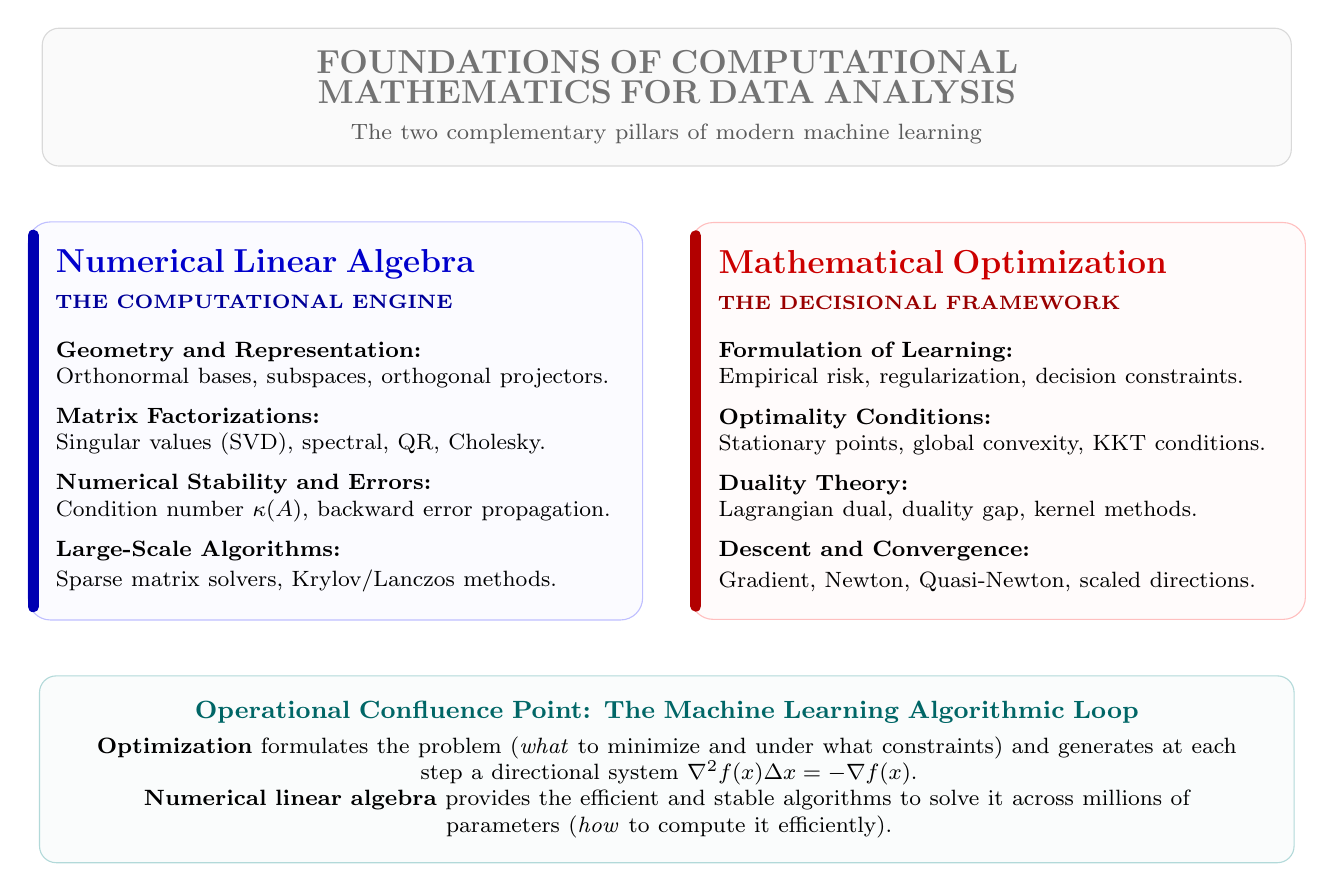
\begin{tikzpicture}[font=\small]

    % Left Pillar Card: anchor=east at (-0.3, 0) ensuring a clean channel
    \node[
        draw=blue!25,
        fill=blue!1.5,
        rounded corners=8pt,
        text width=7.1cm,
        inner sep=10pt,
        align=left,
        anchor=east
    ] (left) at (-0.3, 0) {
        {\large\bfseries\color{blue!80!black} Numerical Linear Algebra}\\[2pt]
        {\scriptsize\bfseries\color{blue!60!black}THE COMPUTATIONAL ENGINE}\\[8pt]
        \footnotesize
        \textbf{Geometry and Representation:}\\
        Orthonormal bases, subspaces, orthogonal projectors.\\[5pt]
        \textbf{Matrix Factorizations:}\\
        Singular values (SVD), spectral, QR, Cholesky.\\[5pt]
        \textbf{Numerical Stability and Errors:}\\
        Condition number $\kappa(A)$, backward error propagation.\\[5pt]
        \textbf{Large-Scale Algorithms:}\\
        Sparse matrix solvers, Krylov/Lanczos methods.
    };

    % Right Pillar Card: anchor=west at (+0.3, 0) ensuring a clean 0.6cm separation
    \node[
        draw=red!25,
        fill=red!1.5,
        rounded corners=8pt,
        text width=7.1cm,
        inner sep=10pt,
        align=left,
        anchor=west
    ] (right) at (0.3, 0) {
        {\large\bfseries\color{red!80!black} Mathematical Optimization}\\[2pt]
        {\scriptsize\color{red!60!black}\bfseries THE DECISIONAL FRAMEWORK}\\[8pt]
        \footnotesize
        \textbf{Formulation of Learning:}\\
        Empirical risk, regularization, decision constraints.\\[5pt]
        \textbf{Optimality Conditions:}\\
        Stationary points, global convexity, KKT conditions.\\[5pt]
        \textbf{Duality Theory:}\\
        Lagrangian dual, duality gap, kernel methods.\\[5pt]
        \textbf{Descent and Convergence:}\\
        Gradient, Newton, Quasi-Newton, scaled directions.
    };

    % Top header: Disciplinary Framing anchored with anchor=south above pillars
    \node[
        draw=gray!30,
        fill=gray!4,
        rounded corners=6pt,
        text width=15.3cm,
        inner sep=8pt,
        align=center,
        anchor=south
    ] (top) at ($(left.north)!0.5!(right.north) + (0, 0.7cm)$) {
        {\large\bfseries\color{gray!90!black} FOUNDATIONS OF COMPUTATIONAL MATHEMATICS FOR DATA ANALYSIS}\\[2pt]
        {\footnotesize\color{gray!70!black}The two complementary pillars of modern machine learning}
    };

    % Bottom integration panel anchored with anchor=north below pillars
    \node[
        draw=teal!30,
        fill=teal!2,
        rounded corners=6pt,
        text width=15.3cm,
        inner sep=9pt,
        align=center,
        anchor=north
    ] (bot) at ($(left.south)!0.5!(right.south) + (0, -0.7cm)$) {
        {\bfseries\color{teal!80!black} Operational Confluence Point: The Machine Learning Algorithmic Loop}\\[4pt]
        \parbox{14.8cm}{\footnotesize\centering
        \textbf{Optimization} formulates the problem (\textit{what} to minimize and under what constraints) and generates at each step a directional system $\nabla^2 f(x) \Delta x = -\nabla f(x)$.\\
        \textbf{Numerical linear algebra} provides the efficient and stable algorithms to solve it across millions of parameters (\textit{how} to compute it efficiently).}
    };

    % Accent stripes on pillars
    \draw[line width=4pt, color=blue!70!black, line cap=round] ($(left.north west)+(2pt,-5pt)$) -- ($(left.south west)+(2pt,5pt)$);
    \draw[line width=4pt, color=red!70!black, line cap=round] ($(right.north west)+(2pt,-5pt)$) -- ($(right.south west)+(2pt,5pt)$);

\end{tikzpicture}%
}
\caption{Synergistic conceptual framework: complementary integration of Numerical Linear Algebra and Mathematical Optimization in Machine Learning.}
\label{fig:pillars-architecture}
\end{figure}

\FloatBarrier
\section{The Philosophy of Mathematical Modeling: Brunelleschi and Galileo}

\subsection{The Genesis of Modeling: From Perspective to Computation}
Extracting actionable insight from massive datasets addresses a fundamental epistemological challenge: raw data is unstructured, cognitively overwhelming, and incapable of making autonomous decisions.

\begin{definition}[Computational Model]
\textbf{Learning (machine learning)} consists of extracting structural regularities from empirical observations and synthesizing them into an abstract mathematical artifact (\textbf{model}), computationally tractable and designed to drive predictions or operational decisions.
\end{definition}

This philosophy has deep historical roots:
\begin{itemize}
    \item \textbf{Filippo Brunelleschi and Perspective:} To erect the free-standing dome of Santa Maria del Fiore in Florence without ground-based wooden falsework, Brunelleschi did not proceed by trial and error on site; he built rigorous mathematical models (geometric projections on an optical cone) capable of predicting radial thrust forces.
    \item \textbf{The Economic Advantage of Mathematics:} Constructing physical scale models (such as wind tunnels in aeronautics) incurs enormous material costs. \textbf{Mathematics costs far less than wood or steel}: equations and algorithms allow simulating billions of operational scenarios at negligible cost.
    \item \textbf{Galileo Galilei and Scientific Abstraction:} Modern physics was born when scientists ceased cataloging every accidental empirical detail and instead abstracted parsimonious mathematical laws expressed in algebraic language.
\end{itemize}

\begin{noteblock}{Definition of a Computational Mathematical Model}
A model is not an identical replica of physical reality. It is an \textbf{abstract mathematical formalization} designed to capture essential causal or correlative patterns while filtering out noise, making the problem tractable on digital computers.
\end{noteblock}

\FloatBarrier
\section{Characterization and Taxonomy of Models}

\subsection{The Triangle of Conflicting Requirements}
Designing any computational model involves balancing three inherently competing objectives:
\begin{enumerate}
    \item \textbf{Accuracy (Accurate):} The fidelity with which the model reflects the actual physical dynamics or behavior of the system.
    \item \textbf{Computational Inexpensiveness (Inexpensive):} Algorithmic simplicity, translating to minimal memory footprints and fast execution times ($\BigO{n}$ or quasi-linear complexity).
    \item \textbf{Generality (General):} The versatility to apply across diverse operational environments and domain distributions.
\end{enumerate}

\begin{property}[Model Incompatibility Principle]
It is theoretically and practically impossible to maximize all three objectives simultaneously: hyper-accurate models require vast parameter counts that destroy computational efficiency; parsimonious, rapid models compromise fine-grained accuracy or generality. Model design is inevitably an \textbf{engineering trade-off}.
\end{property}

\begin{figure}[H]
\centering
\resizebox{0.82\textwidth}{!}{%
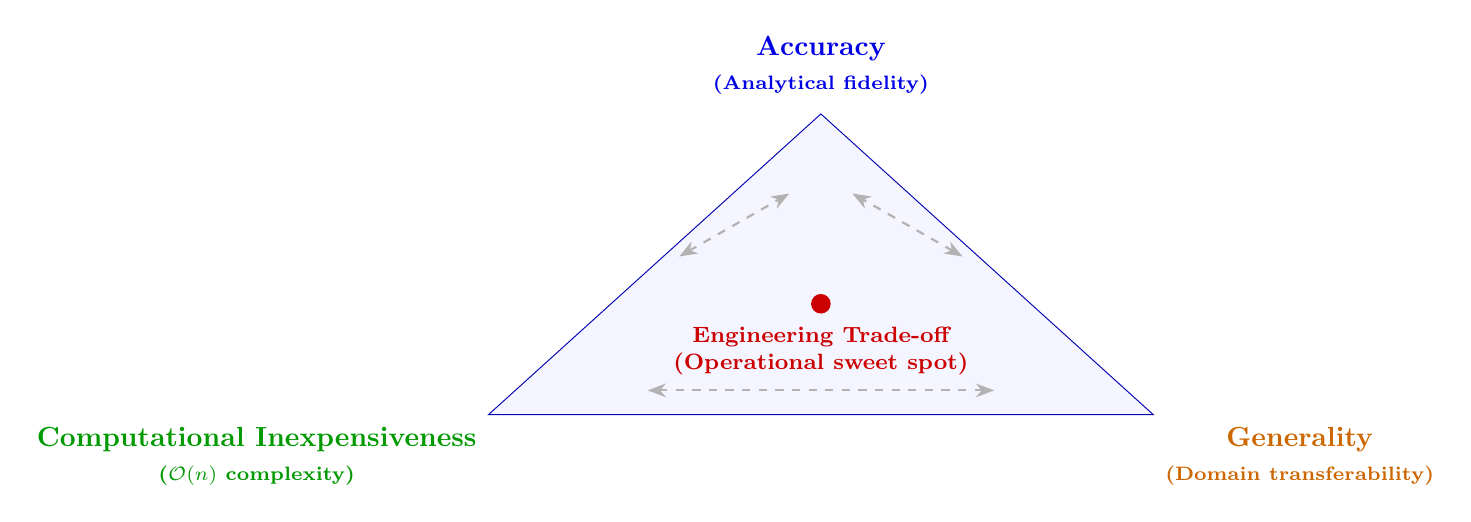
\begin{tikzpicture}[>=Stealth, scale=1.0]
    % Triangle vertices
    \coordinate (A) at (0, 3.8);
    \coordinate (B) at (-4.2, 0);
    \coordinate (C) at (4.2, 0);

    % Outline and fill
    \draw[thick, draw=blue!70!black] (A) -- (B) -- (C) -- cycle;
    \fill[blue!4] (A) -- (B) -- (C) -- cycle;

    % Labels
    \node[above=4pt, font=\bfseries\normalsize, text=blue!90!black, align=center] at (A) {Accuracy\\\scriptsize (Analytical fidelity)};
    \node[below left=2pt, font=\bfseries\normalsize, text=green!60!black, align=center] at (B) {Computational Inexpensiveness\\\scriptsize ($\BigO{n}$ complexity)};
    \node[below right=2pt, font=\bfseries\normalsize, text=orange!80!black, align=center] at (C) {Generality\\\scriptsize (Domain transferability)};

    % Center point
    \node[circle, fill=red!80!black, inner sep=2.5pt] (P) at (0, 1.4) {};
    \node[below=5pt, font=\footnotesize\bfseries, text=red!80!black, align=center] at (P) {Engineering Trade-off\\(Operational sweet spot)};

    % Arrows
    \draw[<->, dashed, gray!60, thick] (-1.8, 2.0) -- (-0.4, 2.8);
    \draw[<->, dashed, gray!60, thick] (1.8, 2.0) -- (0.4, 2.8);
    \draw[<->, dashed, gray!60, thick] (-2.2, 0.3) -- (2.2, 0.3);
\end{tikzpicture}%
}
\caption{The triangle of conflicting requirements in mathematical modeling: accuracy, computational inexpensiveness, and generality.}
\label{fig:model-triangle}
\end{figure}

\subsection{Analytical Models vs Data-Driven (Synthetic) Models}
Table~\ref{tab:model-comparison} outlines the core differences between the two primary modeling paradigms.

\begin{table}[H]
\centering
\small
\begin{tabularx}{\textwidth}{@{} l Y Y @{}}
\toprule
\textbf{Property} & \textbf{Analytical Approach (White-Box)} & \textbf{Data-Driven Approach (Black-Box)} \\
\midrule
\textbf{Principio Base} & Models each individual physical component and its differential interactions. & Does not model internal mechanics; reproduces observed input-output behavior directly. \\
\addlinespace
\textbf{Struttura Matematica} & Flexible, non-linear, derived from first physical principles and conservation laws. & Standardized, rigid, parametric (e.g., deep neural networks, SVMs, linear hyperplanes). \\
\addlinespace
\textbf{Parameters} & Few, calibrated parameters with precise, interpretable physical meaning. & Massive parameter counts (millions to billions), estimated automatically via optimization. \\
\addlinespace
\textbf{Development Cost} & High: requires deep domain expertise and invasive internal system access. & Low/scalable: requires only historical observation logs and standardized optimization solvers. \\
\bottomrule
\end{tabularx}
\caption{Comparison between analytical white-box modeling and empirical data-driven black-box modeling.}
\label{tab:model-comparison}
\end{table}

\subsection{Fitting vs Machine Learning: Empirical Risk and Generalization}
Every model is an approximation (\textit{``the map is not the territory''}):
\begin{itemize}
    \item \textbf{Fitting (Empirical Risk Minimization):} Identifies parameter vectors that minimize discrepancy purely on known observations (\textit{training set}):
    \begin{equation}
        \min_{\mathbf{w}} \mathcal{R}_{\text{emp}}(\mathbf{w}) = \frac{1}{m} \sum_{i=1}^m \ell(f(\mathbf{x}^i; \mathbf{w}), y^i).
    \end{equation}
    \item \textbf{Learning (Generalization):} Requires $f(\mathbf{x}; \mathbf{w})$ to maintain low error on unseen data drawn from the same underlying distribution (\textit{test set}). A hyper-parametrized model that drives training error to zero often suffers from \textbf{overfitting}, fitting spurious noise rather than true underlying relationships.
\end{itemize}

\FloatBarrier
\section{Four Core Mathematical Models in Machine Learning}

\subsection{Example 1: Linear Least Squares Estimation}
Given $m$ observation pairs $(\mathbf{x}^i, y^i) \in \R^n \times \R$, we postulate a linear input-output mapping:
\begin{equation}
    f(\mathbf{x}) = \mathbf{w}^T \mathbf{x} + w_0 = \sum_{j=1}^n w_j x_j + w_0.
\end{equation}
Absorbing the bias $w_0$ into the augmented design matrix $X$:
\begin{equation}
    \mathbf{w}_{\text{ext}} = \begin{bmatrix} w_0 \\ \mathbf{w} \end{bmatrix} \in \R^{n+1}, \quad
    X = \begin{bmatrix} 1 & (\mathbf{x}^1)^T \\ \vdots & \vdots \\ 1 & (\mathbf{x}^m)^T \end{bmatrix} \in \R^{m \times (n+1)}, \quad
    \mathbf{y} = \begin{bmatrix} y^1 \\ \vdots \\ y^m \end{bmatrix} \in \R^m.
\end{equation}
The linear least squares problem minimizes the Euclidean residual:
\begin{equation}
    \min_{\mathbf{w}} \mathcal{L}(\mathbf{w}) = \|\mathbf{y} - X\mathbf{w}\|_2^2 = \mathbf{y}^T \mathbf{y} - 2\mathbf{w}^T X^T \mathbf{y} + \mathbf{w}^T X^T X \mathbf{w}.
\end{equation}
Setting the gradient $\nabla \mathcal{L}(\mathbf{w})$ to zero yields the stationary condition, known as the \textbf{Gauss Normal Equations}:
\begin{equation}
    \nabla \mathcal{L}(\mathbf{w}) = -2 X^T \mathbf{y} + 2 X^T X \mathbf{w} = \mathbf{0} \implies X^T X \mathbf{w} = X^T \mathbf{y}.
\end{equation}
When $X$ has full column rank ($\rank(X) = n+1$), $X^T X$ is symmetric positive definite and invertible:
\begin{equation}
    \mathbf{w}^* = (X^T X)^{-1} X^T \mathbf{y}.
\end{equation}

\begin{alertblock}{Golden Numerical Rule: Never Compute $(X^T X)^{-1}$ Explicitly}
In scientific computing, \textbf{one must never explicitly form $X^T X$ nor compute its inverse}. Multiplying $X^TX$ squares the condition number ($\kappa(X^T X) = \kappa(X)^2$), drastically magnifying floating-point roundoff errors. The system is solved stably using QR factorization or truncated SVD (backslash operator in GNU Octave: \texttt{w = X \textbackslash\ y}).
\end{alertblock}

\subsection{Example 2: Low-Rank Approximation and Recommender Systems}
Given a partially observed data matrix $M \in \R^{n \times m}$ (e.g., $n$ users and $m$ movies, with $M_{ij}$ indicating ratings), we seek a low-rank factorization $k \ll \min(n, m)$ such that $M \approx AB$:
\begin{equation}
    A \in \R^{n \times k}, \quad B \in \R^{k \times m} \implies \min_{A, B} \|M - AB\|_F^2 = \sum_{i=1}^n \sum_{j=1}^m (M_{ij} - (AB)_{ij})^2.
\end{equation}

\begin{figure}[H]
\centering
\resizebox{0.92\textwidth}{!}{%
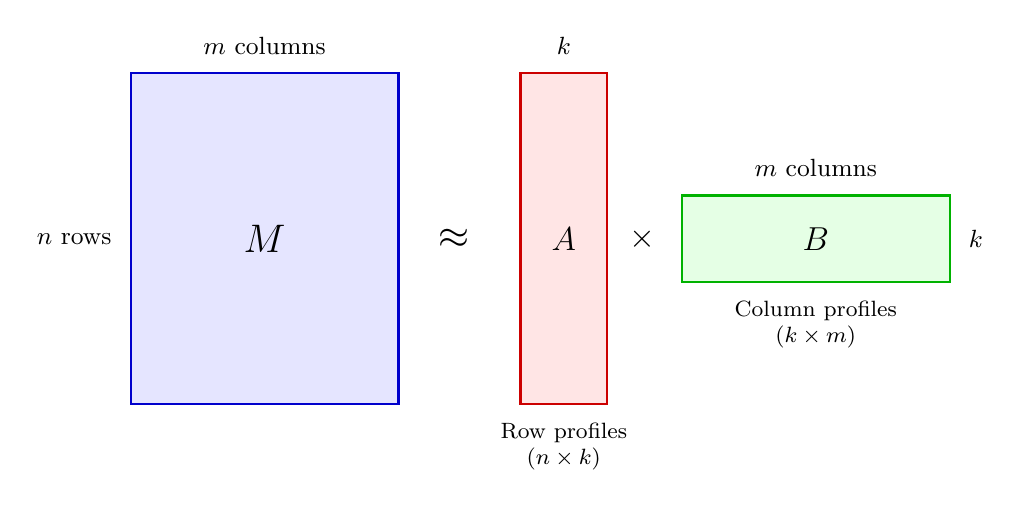
\begin{tikzpicture}[>=Stealth]
    % Matrix M
    \node[draw=blue!80!black, fill=blue!10, thick, minimum width=3.4cm, minimum height=4.2cm] (M) at (0, 0) {};
    \node[font=\bfseries\Large] at (0, 0) {$M$};
    \node[above=3pt, font=\small] at (M.north) {$m$ columns};
    \node[left=3pt, font=\small] at (M.west) {$n$ rows};

    \node[font=\Large] at (2.4, 0) {$\approx$};

    % Matrix A
    \node[draw=red!80!black, fill=red!10, thick, minimum width=1.1cm, minimum height=4.2cm] (A) at (3.8, 0) {};
    \node[font=\bfseries\large] at (3.8, 0) {$A$};
    \node[above=3pt, font=\small] at (A.north) {$k$};
    \node[below=3pt, font=\footnotesize, align=center] at (A.south) {Row profiles\\($n \times k$)};

    \node[font=\large] at (4.8, 0) {$\times$};

    % Matrix B
    \node[draw=green!70!black, fill=green!10, thick, minimum width=3.4cm, minimum height=1.1cm] (B) at (7.0, 0) {};
    \node[font=\bfseries\large] at (7.0, 0) {$B$};
    \node[right=3pt, font=\small] at (B.east) {$k$};
    \node[above=3pt, font=\small] at (B.north) {$m$ columns};
    \node[below=3pt, font=\footnotesize, align=center] at (B.south) {Column profiles\\($k \times m$)};
\end{tikzpicture}%
}
\caption{Low-rank matrix factorization: compressing storage from $nm$ entries to $k(n + m)$.}
\label{fig:low-rank-matrix}
\end{figure}

\subsubsection{Memory Compression and Spectral Properties}
Storing $M$ explicitly requires $n \cdot m$ memory entries; storing $A$ and $B$ requires $k(n + m)$. For $n = 10^6$, $m = 10^5$, and rank $k = 10$:
\begin{align}
    \text{Raw storage} &= 10^6 \times 10^5 = 10^{11} \text{ cells}, \\
    \text{Factorized storage} &= 10 \times (10^6 + 10^5) \approx 1.1 \times 10^7 \text{ cells},
\end{align}
achieving a \textbf{99.99\% storage reduction}.

By the Eckart-Young-Mirsky Theorem, the optimal low-rank matrix under the Frobenius norm is given by the truncated Singular Value Decomposition (SVD).

\begin{alertblock}{Computational Warning on Sparse Matrices}
When $M$ is sparse, \textbf{one must never form $M^T M$ or $M M^T$}. Matrix multiplication destroys sparsity, producing a dense matrix that triggers immediate Out-Of-Memory (OOM) failures. One must rely exclusively on iterative methods using matrix-vector products (Lanczos bidiagonalization).
\end{alertblock}

\subsection{Example 3: Support Vector Machines (SVM) --- Margin, Duality, and Kernels}
For binary classification with labels $y^h \in \{-1, +1\}$, a linear classifier makes predictions via $\hat{y} = \operatorname{sign}(\mathbf{w}_+^T \mathbf{x} - w_0)$.

\begin{figure}[H]
\centering
\resizebox{0.82\textwidth}{!}{%
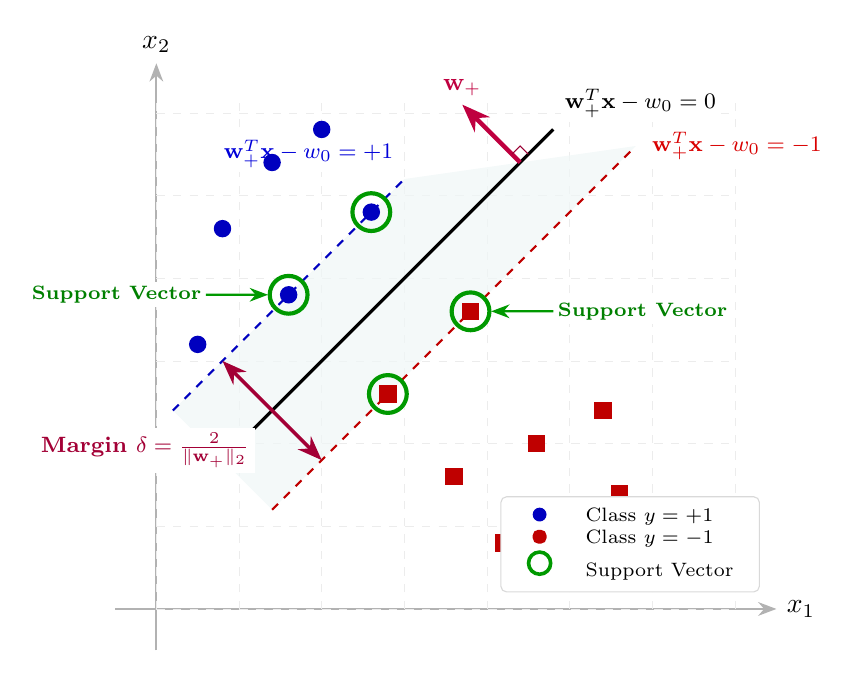
\begin{tikzpicture}[>=Stealth, scale=1.05]
    % Axes
    \draw[->, thick, gray!60] (-0.5, 0) -- (7.5, 0) node[right, black] {$x_1$};
    \draw[->, thick, gray!60] (0, -0.5) -- (0, 6.6) node[above, black] {$x_2$};
    \draw[help lines, color=gray!15, dashed] (0,0) grid (7.0,6.2);

    % Margin corridor (shaded background)
    \fill[teal!6, opacity=0.7] (0.2, 2.4) -- (3.0, 5.2) -- (5.8, 5.6) -- (1.4, 1.2) -- cycle;

    % Upper margin hyperplane (+1): x2 = x1 + 2.2
    \draw[dashed, thick, draw=blue!75!black] (0.2, 2.4) -- (3.0, 5.2) 
        node[above left=3pt, font=\footnotesize\bfseries, blue!85!black, fill=white, inner sep=1.5pt] {$\mathbf{w}_+^T \mathbf{x} - w_0 = +1$};

    % Optimal separating hyperplane (w^T x - w_0 = 0): x2 = x1 + 1.0
    \draw[very thick, draw=black] (0.8, 1.8) -- (4.8, 5.8) 
        node[above right=3pt, font=\footnotesize\bfseries, black, fill=white, inner sep=1.5pt] {$\mathbf{w}_+^T \mathbf{x} - w_0 = 0$};

    % Lower margin hyperplane (-1): x2 = x1 - 0.2
    \draw[dashed, thick, draw=red!75!black] (1.4, 1.2) -- (5.8, 5.6) 
        node[right=4pt, font=\footnotesize\bfseries, red!85!black, fill=white, inner sep=1.5pt] {$\mathbf{w}_+^T \mathbf{x} - w_0 = -1$};

    % Class +1 interior points (blue circles)
    \foreach \coord in {(0.8, 4.6), (1.4, 5.4), (2.0, 5.8), (0.5, 3.2)} {
        \fill[blue!75!black] \coord circle (3.0pt);
    }

    % Class -1 interior points (red squares)
    \foreach \coord in {(3.6, 1.6), (4.6, 2.0), (5.4, 2.4), (4.2, 0.8), (5.6, 1.4)} {
        \fill[red!75!black] \coord +(-3.0pt,-3.0pt) rectangle +(3.0pt,3.0pt);
    }

    % Support Vectors (strictly on supporting hyperplanes)
    % On H+1: (1.6, 3.8) and (2.6, 4.8)
    \fill[blue!75!black] (1.6, 3.8) circle (3.0pt);
    \draw[line width=1.5pt, green!60!black] (1.6, 3.8) circle (6.5pt);

    \fill[blue!75!black] (2.6, 4.8) circle (3.0pt);
    \draw[line width=1.5pt, green!60!black] (2.6, 4.8) circle (6.5pt);

    % On H-1: (2.8, 2.6) and (3.8, 3.6)
    \fill[red!75!black] (2.8, 2.6) +(-3.0pt,-3.0pt) rectangle +(3.0pt,3.0pt);
    \draw[line width=1.5pt, green!60!black] (2.8, 2.6) circle (6.5pt);

    \fill[red!75!black] (3.8, 3.6) +(-3.0pt,-3.0pt) rectangle +(3.0pt,3.0pt);
    \draw[line width=1.5pt, green!60!black] (3.8, 3.6) circle (6.5pt);

    % Support Vector callouts with clean horizontal pointers
    \node[anchor=east, font=\scriptsize\bfseries, green!50!black, fill=white, inner sep=1.5pt] (sv1) at (0.6, 3.8) {Support Vector};
    \draw[->, thick, green!60!black] (sv1.east) -- (1.35, 3.8);

    \node[anchor=west, font=\scriptsize\bfseries, green!50!black, fill=white, inner sep=1.5pt] (sv2) at (4.8, 3.6) {Support Vector};
    \draw[->, thick, green!60!black] (sv2.west) -- (4.05, 3.6);

    % Normal vector w_+ orthogonal to decision boundary
    \draw[->, ultra thick, purple] (4.4, 5.4) -- (3.7, 6.1);
    \node[above=2pt, font=\small\bfseries, purple, fill=white, inner sep=1pt] at (3.7, 6.1) {$\mathbf{w}_+$};
    \draw[purple!80!black, thin] (4.4, 5.4) +(-0.1, 0.1) -- +(-0.0, 0.2) -- +(0.1, 0.1);

    % Margin width (orthogonal distance between H-1 and H+1)
    \draw[<->, line width=1.3pt, purple!85!black] (2.0, 1.8) -- (0.8, 3.0);
    \node[anchor=north east, font=\footnotesize\bfseries, purple!85!black, fill=white, inner sep=2pt] at (1.2, 2.2) {Margin $\delta = \frac{2}{\|\mathbf{w}_+\|_2}$};

    % Legend
    \node[draw=gray!30, fill=white, rounded corners=2pt, font=\scriptsize, anchor=south east] at (7.3, 0.2) {
        \begin{tabular}{cl}
        \tikz\fill[blue!75!black] (0,0) circle (2.5pt); & Class $y = +1$ \\
        \tikz\fill[red!75!black] (-2.5pt,-2.5pt) rectangle (2.5pt,2.5pt); & Class $y = -1$ \\
        \tikz\draw[line width=1.3pt, green!60!black] (0,0) circle (4pt); & Support Vector
        \end{tabular}
    };
\end{tikzpicture}%
}
\caption{Margin geometry in linear Support Vector Machines: maximizing the separation distance between supporting hyperplanes.}
\label{fig:svm-margin}
\end{figure}

Maximizing the geometric margin $2/\|\mathbf{w}_+\|_2$ is equivalent to minimizing $\|\mathbf{w}_+\|_2^2$:
\begin{equation}
    \min_{\mathbf{w}_+, w_0} \frac{1}{2} \|\mathbf{w}_+\|_2^2 \qquad \text{s.t.} \quad y^h (\mathbf{w}_+^T \mathbf{x}^h - w_0) \ge 1 \quad \forall h = 1, \dots, m.
\end{equation}

For non-linearly separable data, slack variables $\xi_h \ge 0$ yield the \textbf{Soft Margin} problem:
\begin{equation}
\begin{aligned}
    \min_{\mathbf{w}_+, w_0, \boldsymbol{\xi}} \quad & \frac{1}{2} \|\mathbf{w}_+\|_2^2 + C \sum_{h=1}^m \xi_h \\
    \text{s.t.} \quad & y^h (\mathbf{w}_+^T \mathbf{x}^h - w_0) \ge 1 - \xi_h, \quad \xi_h \ge 0 \quad \forall h=1, \dots, m.
\end{aligned}
\end{equation}
Parameter $C > 0$ controls the trade-off between margin width and classification violations: $C \to \infty$ forces hard separation, while moderate values allow controlled margin errors to protect test generalization.

\subsubsection{Non-Linear Lifting, Duality, and the Kernel Trick}
When points are not linearly separable in $\R^n$, a non-linear mapping $\boldsymbol{\phi}: \R^n \to \mathcal{H}$ lifts data into a higher-dimensional feature space:
\begin{equation}
    \mathbf{x} \mapsto \boldsymbol{\phi}(\mathbf{x}).
\end{equation}
The Wolfe dual problem is given by:
\begin{equation}
\begin{aligned}
    \max_{\boldsymbol{\alpha}} \quad & \sum_{h=1}^m \alpha_h - \frac{1}{2} \sum_{h=1}^m \sum_{k=1}^m \alpha_h \alpha_k y^h y^k \langle \boldsymbol{\phi}(\mathbf{x}^h), \boldsymbol{\phi}(\mathbf{x}^k) \rangle_{\mathcal{H}} \\
    \text{s.t.} \quad & \sum_{h=1}^m y^h \alpha_h = 0, \quad 0 \le \alpha_h \le C \quad \forall h=1, \dots, m.
\end{aligned}
\end{equation}
Because data points appear solely through inner products, Mercer's Theorem permits evaluating them via a \textbf{kernel function} $K(\mathbf{x}^h, \mathbf{x}^k) = \langle \boldsymbol{\phi}(\mathbf{x}^h), \boldsymbol{\phi}(\mathbf{x}^k) \rangle_{\mathcal{H}}$. For example, the \textbf{Gaussian RBF Kernel}:
\begin{equation}
    K(\mathbf{x}, \mathbf{z}) = \exp\left(-\gamma \|\mathbf{x} - \mathbf{z}\|_2^2\right)
\end{equation}
corresponds to an infinite-dimensional Hilbert space $\mathcal{H}$, evaluated in $\BigO{n}$ time without ever forming $\boldsymbol{\phi}(\mathbf{x})$ explicitly.

\subsection{Example 4: Clustering and the K-Means Algorithm}
Given an unlabelled dataset $X = \{\mathbf{x}^1, \dots, \mathbf{x}^m\} \subset \R^h$, clustering seeks to partition $X$ into $k$ disjoint subsets $\{X_p\}_{p=1}^k$ maximizing intra-cluster cohesion.

\subsubsection{Biconvex Optimization Formulation}
Introducing $k$ cluster centroids $\mathbf{c}^1, \dots, \mathbf{c}^k \in \R^h$ and binary assignment variables $z_{ip} \in \{0, 1\}$:
\begin{equation}
    \min_{\mathbf{c}, Z} \sum_{i=1}^m \sum_{p=1}^k z_{ip} \|\mathbf{c}^p - \mathbf{x}^i\|_2^2 \qquad \text{s.t.} \quad \sum_{p=1}^k z_{ip} = 1 \; \forall i, \quad z_{ip} \in \{0, 1\} \; \forall i,p.
\end{equation}
The problem is non-convex due to binary integrality $z_{ip} \in \{0, 1\}$ and bilinear terms $z_{ip}\mathbf{c}^p$. However, its biconvex structure enables \textbf{Block Gauss-Seidel alternating optimization}:
\begin{enumerate}
    \item \textbf{Fixing $\mathbf{c}$, optimize $Z$:} Each point is assigned to its nearest Euclidean centroid ($z_{i\bar{p}} = 1 \iff \bar{p} = \arg\min_p \|\mathbf{c}^p - \mathbf{x}^i\|_2^2$).
    \item \textbf{Fixing $Z$, optimize $\mathbf{c}$:} Vanishing the convex quadratic gradient with respect to $\mathbf{c}^p$:
    \begin{equation}
        2 \sum_{i \in I(p)} (\mathbf{c}^p - \mathbf{x}^i) = \mathbf{0} \implies (\mathbf{c}^p)^* = \frac{1}{|I(p)|} \sum_{i \in I(p)} \mathbf{x}^i.
    \end{equation}
    The optimal centroid is the \textbf{vector mean (barycenter)} of all points belonging to cluster $p$.
\end{enumerate}

\begin{algorithm}[H]
\caption{K-Means Algorithm for Euclidean Clustering}\label{alg:kmeans-en}
\KwInput{Dataset $X = \{\mathbf{x}^1, \dots, \mathbf{x}^m\} \subset \R^h$, number of clusters $k$, initial centroids $\mathbf{c}^1, \dots, \mathbf{c}^k$, tolerance $\epsilon > 0$}
\KwOutput{Final centroids $\mathbf{c}^1, \dots, \mathbf{c}^k$ and partition $\{I(p)\}_{p=1}^k$}
$v \leftarrow \infty$\;
\Repeat{$(v - v_{\mathrm{new}}) \le \epsilon$}{
    \tcp{Step 1: Point assignment to nearest centroid}
    \For{$p \leftarrow 1$ \KwTo $k$}{
        $I(p) \leftarrow \emptyset$\;
    }
    \For{$i \leftarrow 1$ \KwTo $m$}{
        $p^* \leftarrow \arg\min_{p \in \{1, \dots, k\}} \|\mathbf{c}^p - \mathbf{x}^i\|_2^2$\;
        $I(p^*) \leftarrow I(p^*) \cup \{i\}$\;
    }
    \tcp{Step 2: Centroid re-computation (mean)}
    \For{$p \leftarrow 1$ \KwTo $k$}{
        \If{$I(p) \neq \emptyset$}{
            $\mathbf{c}^p \leftarrow \frac{1}{|I(p)|} \sum_{i \in I(p)} \mathbf{x}^i$\;
        }
    }
    \tcp{Step 3: Objective value evaluation}
    $v_{\mathrm{new}} \leftarrow \sum_{p=1}^k \sum_{i \in I(p)} \|\mathbf{c}^p - \mathbf{x}^i\|_2^2$\;
    $v \leftarrow v_{\mathrm{new}}$\;
}
\Return{$\mathbf{c}^1, \dots, \mathbf{c}^k$}\;
\end{algorithm}

\begin{noteblock}{Why Scientific Computing Violates Agile Modularity}
In standard software engineering (Agile), systems are decomposed into decoupled, independently swappable modules. In scientific computing, this separation fails:
\begin{itemize}
    \item Replacing the Euclidean metric $\ell_2$ with the Manhattan distance $\ell_1$ completely changes the closed-form centroid: the $\ell_1$ optimum is no longer the arithmetic mean, but the \textbf{component-wise median}.
    \item The tight interdependence between loss formulation and update routines demands an integrated, holistic mathematical design.
\end{itemize}
\end{noteblock}

\FloatBarrier
\section{Methodological Principles of Computational Learning}

\subsection{The ``Magic Academy'' Metaphor}
To illustrate the difference between superficial library usage and rigorous computational competence, consider the \textbf{Magic Academy}:
\begin{itemize}
    \item \textbf{The Sorcerer's Apprentice (\textit{Black-Box Practitioner}):} Invokes library routines (\texttt{import sklearn}, \texttt{fit()}) as pre-packaged incantations. In nominal conditions, output appears satisfactory; however, when confronted with numerical instability or ill-conditioning, they lack the insight required to diagnose the root cause.
    \item \textbf{The Master Magician (\textit{Computational Scientist}):} Understands spectral properties and convergence theory, detects ill-posed systems, tracks floating-point error amplification, and replaces fragile algorithms with robust, numerically sound alternatives.
\end{itemize}

\subsection{The Three Guiding Principles of Machine Learning}
\begin{enumerate}
    \item \textbf{Learning is Numerical Computation:} Every AI algorithm fundamentally reduces to solving a linear algebraic system or minimizing an objective loss function.
    \item \textbf{The Dimensional Scale Challenge:} Machine learning problems are rarely mathematically intractable; they are predominantly linear, convex, or quadratic. \textbf{Their difficulty stems entirely from their colossal scale} (\textit{«hard because large, not hard because hard»}), spanning millions to billions of parameters.
    \item \textbf{Linear Algebra as the Engine of Optimization:} Optimizing at extreme scales demands ruthless hardware efficiency: numerical linear algebra provides the computational engine that makes optimization fast, scalable, and numerically stable.
\end{enumerate}

\FloatBarrier
\section{Synoptic Formula Reference of Introductory Models}

Table~\ref{tab:model-summary-en} summarizes the foundational mathematical formulations and their computational paradigms.

\begin{table}[H]
\centering
\footnotesize
\begin{tabularx}{\textwidth}{@{} >{\bfseries}l >{\raggedright\arraybackslash}p{3.8cm} >{\raggedright\arraybackslash}p{3.1cm} Y @{}}
\toprule
\normalfont\textbf{Model} & \textbf{Formulation} & \textbf{Paradigm} & \textbf{Computational Notes} \\
\midrule
Least Squares & $\min_{\mathbf{w}} \|\mathbf{y} - X\mathbf{w}\|_2^2$ & Normal equations:\newline $\mathbf{w}^* = (X^TX)^{-1}X^T\mathbf{y}$ & Solve via QR factorization; never invert $X^TX$ explicitly. \\
\addlinespace[2pt]
Low-Rank & $\min_{A, B} \|M - AB\|_F^2$ & Truncated SVD (Eckart-Young) & Compression $nm \to k(n+m)$; avoid Gramian $M^TM$ on sparse data. \\
\addlinespace[2pt]
SVM (Hard) & $\min \frac{1}{2}\|\mathbf{w}_+\|_2^2$\newline $\text{s.t. } y^h(\mathbf{w}_+^T\mathbf{x}^h - w_0) \ge 1$ & Convex Quadratic Program (QP) & Maximizes geometric margin $2/\|\mathbf{w}_+\|_2$ under strict separation. \\
\addlinespace[2pt]
SVM (Soft) & $\min \frac{1}{2}\|\mathbf{w}_+\|_2^2 + C \sum \xi_h$\newline $\text{s.t. } y^h(\mathbf{w}_+^T\mathbf{x}^h - w_0) \ge 1-\xi_h$ & QP with linear constraints (equivalent to Hinge loss) & Trade-off parameter $C > 0$ balances bias-variance via slack variables. \\
\addlinespace[2pt]
SVM (Kernel) & $\max_{\boldsymbol{\alpha}} \mathbf{1}^T\boldsymbol{\alpha} - \frac{1}{2}\boldsymbol{\alpha}^T \tilde{K} \boldsymbol{\alpha}$\newline $\text{s.t. } \mathbf{y}^T\boldsymbol{\alpha}=0, \; 0 \le \alpha_h \le C$ & QP with box constraints & Inner products in infinite-dimensional Hilbert spaces (RBF) in $\BigO{n}$. \\
\addlinespace[2pt]
K-Means & $\min \sum_{i,p} z_{ip} \|\mathbf{c}^p - \mathbf{x}^i\|_2^2$\newline $\text{s.t. } \sum_p z_{ip}=1, \; z_{ip}\in\{0,1\}$ & Alternating minimization (Block Gauss-Seidel) & Finite convergence to local minimum; cluster centroids given in closed form. \\
\bottomrule
\end{tabularx}
\caption{Synoptic reference of introductory mathematical models and computational properties.}
\label{tab:model-summary-en}
\end{table}


% ========================================================
% PART I: NUMERICAL LINEAR ALGEBRA AND DATA ANALYSIS
% ========================================================
\part{Numerical Linear Algebra and Data Analysis}
\chapter{Linear Algebra Review: Vectors, Norms, Bases, and Transformations}
\label{chap:linear-algebra-review-vectors-norms}

\FloatBarrier
\section{Introduction to Numerical Computation and Applied Motivations}

This course addresses the computational and efficient resolution of linear algebra problems on digital computers~\cite{trefethen1997numerical,golub2013matrix}. In applied mathematics, data science, and machine learning, the general formulation of a decision problem typically takes the form of an optimization task:
\begin{equation}
    \min_{\mathbf{x} \in S} f(\mathbf{x}),
\end{equation}
where $f: \R^n \to \R$ denotes the objective function and $S \subseteq \R^n$ defines the feasible set of constraints.

Within numerical linear algebra, this general problem is frequently reformulated or locally approximated by a linear least squares problem:
\begin{equation}
    \min_{\mathbf{x} \in \R^n} \|A \mathbf{x} - \mathbf{b}\|_2^2,
\end{equation}
where $A \in \R^{m \times n}$ represents the model or design matrix, $\mathbf{b} \in \R^m$ the observed target vector, and $\mathbf{x} \in \R^n$ the unknown parameter vector to estimate.

\begin{noteblock}{Why Focus on Linear Problems?}
Key motivations establishing linear problems as fundamental to scientific computing include:
\begin{enumerate}
    \item \textbf{Theoretical tractability and analytical clarity:} Linear problems exhibit clean, well-understood algebraic structures, enabling rigorous guarantees on existence, uniqueness, and algorithm convergence.
    \item \textbf{Efficiency and machine accuracy:} Specialized direct and iterative algorithms can compute solutions up to the limits of machine floating-point arithmetic (IEEE 754 standard, $\epsilon_{\text{mach}} \approx 10^{-16}$ in double precision).
    \item \textbf{Exploitation of special matrix structures:} Matrices endowed with specific properties (symmetric, positive definite, orthogonal, banded, Toeplitz, or sparse) permit specialized algorithms with significantly reduced asymptotic and memory complexity.
    \item \textbf{Building blocks for non-linear algorithms:} Nearly all sophisticated numerical methods for non-linear problems (Newton's method, Quasi-Newton schemes like BFGS, constrained optimization, and PDE solvers) solve one or more linear systems or least squares subproblems at every iteration.
    \item \textbf{Stability and error control:} Numerical practitioners demand algorithms resilient against catastrophic round-off error accumulation and algorithmic instability.
\end{enumerate}
\end{noteblock}

\FloatBarrier
\section{Vectors, Vector Spaces, and Geometric Representation}

\subsection{Notation and Conventions}

Unless stated otherwise, \textbf{all vectors are assumed to be column vectors}. A vector $\mathbf{x} \in \R^n$ is denoted:
\begin{equation}
    \mathbf{x} = \begin{bmatrix} x_1 \\ x_2 \\ \vdots \\ x_n \end{bmatrix}, \qquad \mathbf{x}^T = \begin{bmatrix} x_1 & x_2 & \dots & x_n \end{bmatrix}.
\end{equation}

Consider, for example in $\R^2$, the two vectors:
\begin{equation}
    \mathbf{x} = \begin{bmatrix} 2 \\ 4 \end{bmatrix}, \qquad \mathbf{y} = \begin{bmatrix} 2 \\ 1 \end{bmatrix}.
\end{equation}

The fundamental operation defining vector space addition is component-wise summation:
\begin{equation}
    \mathbf{x} + \mathbf{y} = \begin{bmatrix} 2 \\ 4 \end{bmatrix} + \begin{bmatrix} 2 \\ 1 \end{bmatrix} = \begin{bmatrix} 2+2 \\ 4+1 \end{bmatrix} = \begin{bmatrix} 4 \\ 5 \end{bmatrix}.
\end{equation}

\subsection{Geometric Interpretation: Points, Arrows, and the Parallelogram Rule}

A vector $\mathbf{x} = [x_1, x_2]^T \in \R^2$ admits two complementary geometric perspectives:
\begin{itemize}
    \item as a \textbf{point} in the Cartesian plane with coordinates $(x_1, x_2)$ relative to the origin;
    \item as a \textbf{directed segment (arrow)} originating at $(0,0)$ and terminating at $(x_1, x_2)$.
\end{itemize}

Vector addition $\mathbf{x} + \mathbf{y}$ corresponds to the classical \textbf{parallelogram law}: translating the tail of $\mathbf{y}$ to the tip of $\mathbf{x}$, the resulting vector connects the origin to the opposite vertex of the parallelogram formed by the two vectors, terminating at $(4, 5)$. This notion generalizes directly to $n$-dimensional Euclidean spaces $\R^n$ ($n \ge 3$).

\begin{figure}[H]
\centering
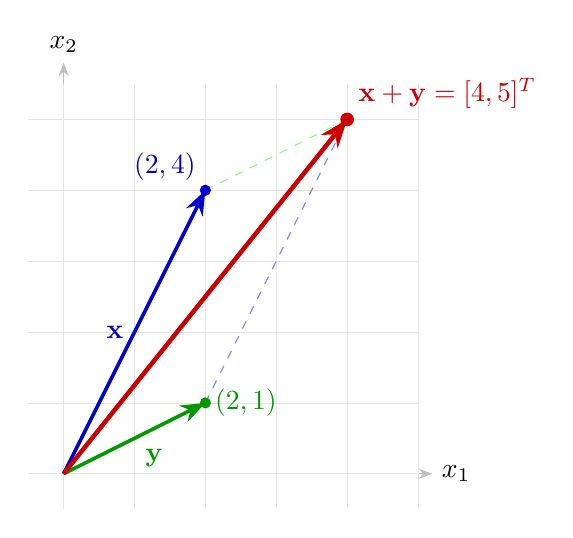
\begin{tikzpicture}[scale=0.9, >=Stealth]
    \draw[->, gray!50, thin] (-0.5,0) -- (5.2,0) node[right, black] {$x_1$};
    \draw[->, gray!50, thin] (0,-0.5) -- (0,5.8) node[above, black] {$x_2$};
    \draw[step=1.0, gray!20, very thin] (-0.5,-0.5) grid (5.0,5.5);

    % Vectors x and y
    \draw[->, line width=1.3pt, blue!80!black] (0,0) -- (2,4) node[midway, left] {$\mathbf{x}$};
    \draw[->, line width=1.3pt, green!60!black] (0,0) -- (2,1) node[midway, below right] {$\mathbf{y}$};

    % Dashed parallelogram lines
    \draw[dashed, blue!50] (2,1) -- (4,5);
    \draw[dashed, green!50] (2,4) -- (4,5);

    % Sum vector
    \draw[->, line width=1.6pt, red!80!black] (0,0) -- (4,5) node[above right] {$\mathbf{x} + \mathbf{y} = [4, 5]^T$};

    % Terminal points
    \filldraw[blue!80!black] (2,4) circle (2pt) node[above left] {$(2,4)$};
    \filldraw[green!60!black] (2,1) circle (2pt) node[right] {$(2,1)$};
    \filldraw[red!80!black] (4,5) circle (2.5pt);
\end{tikzpicture}
\caption{Geometric interpretation of vector addition in $\R^2$ via the parallelogram rule.}
\label{fig:parallelogram-rule-en}
\end{figure}

\subsection{Measuring the ``Size'' of a Vector}

Consider the following question:
\begin{quote}
    \textit{Given the vectors $\mathbf{v}, \mathbf{w} \in \R^4$:}
    \begin{equation}
        \mathbf{v} = \begin{bmatrix} 2 \\ 2 \\ 2 \\ 2 \end{bmatrix}, \qquad \mathbf{w} = \begin{bmatrix} 4 \\ 0 \\ 0 \\ 0 \end{bmatrix},
    \end{equation}
    \textit{which of these two vectors is ``larger''?}
\end{quote}

The question is fundamentally ill-posed until a precise formal criterion of measurement is chosen:
\begin{itemize}
    \item Looking at the \textbf{maximum individual component}, $\mathbf{w}$ contains an entry of $4$, whereas all entries of $\mathbf{v}$ are $2$.
    \item Looking at the \textbf{sum of components}, $\mathbf{v}$ sums to $2 + 2 + 2 + 2 = 8$, while $\mathbf{w}$ only reaches $4$.
    \item Looking at the \textbf{Euclidean geometric length}, both measure $\sqrt{16} = 4$.
\end{itemize}

To answer such questions unequivocally, the formal concept of a \textbf{vector norm} is required.

\FloatBarrier
\section{Vector Norms and Normed Spaces}

\begin{definition}[Vector Norm]
Let $V$ be a real (or complex) vector space. A function $\|\cdot\|: V \to \R$ is called a \textbf{vector norm} if and only if it satisfies the following three axioms for all $\mathbf{v}, \mathbf{w} \in V$ and every scalar $\lambda \in \R$:
\begin{enumerate}
    \item \textbf{Non-negativity and positive definiteness:}
    \begin{equation}
        \|\mathbf{v}\| \ge 0 \quad \forall \mathbf{v} \in V, \qquad \|\mathbf{v}\| = 0 \iff \mathbf{v} = \mathbf{0}_V.
    \end{equation}
    \item \textbf{Absolute homogeneity:}
    \begin{equation}
        \|\lambda \mathbf{v}\| = |\lambda| \cdot \|\mathbf{v}\| \quad \forall \lambda \in \R, \; \forall \mathbf{v} \in V.
    \end{equation}
    \item \textbf{Triangle inequality:}
    \begin{equation}
        \|\mathbf{v} + \mathbf{w}\| \le \|\mathbf{v}\| + \|\mathbf{w}\| \quad \forall \mathbf{v}, \mathbf{w} \in V.
    \end{equation}
\end{enumerate}
\end{definition}

A vector space $V$ paired with a norm $\|\cdot\|$ is termed a \textbf{normed space}.

\subsection{The \texorpdfstring{$\ell_p$}{lp}-Norm Family on \texorpdfstring{$\R^n$}{Rn}}

Let $\mathbf{v} = [v_1, v_2, \dots, v_n]^T \in \R^n$. The norms most commonly employed in numerical analysis and machine learning belong to the parameterized $\ell_p$-norm family:
\begin{equation}
    \|\mathbf{v}\|_p = \left( \sum_{i=1}^n |v_i|^p \right)^{1/p} \qquad (p \ge 1).
\end{equation}

Three canonical special cases are:

\paragraph{1. Euclidean Norm ($\ell_2$).}
Represents standard geometric distance in Euclidean affine space:
\begin{equation}
    \|\mathbf{v}\|_2 = \sqrt{\sum_{i=1}^n v_i^2} = \sqrt{\mathbf{v}^T \mathbf{v}}.
\end{equation}

\paragraph{2. Manhattan Norm ($\ell_1$ or Taxi-cab).}
Sums the absolute values of all coordinates:
\begin{equation}
    \|\mathbf{v}\|_1 = \sum_{i=1}^n |v_i|.
\end{equation}

\paragraph{3. Maximum Norm ($\ell_\infty$ or Chebyshev Norm).}
Captures the largest absolute component:
\begin{equation}
    \|\mathbf{v}\|_\infty = \lim_{p \to \infty} \|\mathbf{v}\|_p = \max_{1 \le i \le n} |v_i|.
\end{equation}

\subsection{Rigorous Comparison of Vectors \texorpdfstring{$\mathbf{v}$}{v} and \texorpdfstring{$\mathbf{w}$}{w}}

Revisiting vectors $\mathbf{v} = [2, 2, 2, 2]^T$ and $\mathbf{w} = [4, 0, 0, 0]^T \in \R^4$:

\begin{example}[Comparative Evaluation Across the Three Norms]
\mbox{}\par\nopagebreak
\begin{itemize}
    \item \textbf{In Euclidean $\ell_2$ norm:}
    \begin{align}
        \|\mathbf{v}\|_2 &= \sqrt{2^2 + 2^2 + 2^2 + 2^2} = \sqrt{16} = 4, \\
        \|\mathbf{w}\|_2 &= \sqrt{4^2 + 0^2 + 0^2 + 0^2} = \sqrt{16} = 4.
    \end{align}
    The two vectors have the exact same \textbf{Euclidean length}: $\|\mathbf{v}\|_2 = \|\mathbf{w}\|_2 = 4$.
    \item \textbf{In $\ell_1$ norm:}
    \begin{align}
        \|\mathbf{v}\|_1 &= |2| + |2| + |2| + |2| = 8, \\
        \|\mathbf{w}\|_1 &= |4| + |0| + |0| + |0| = 4.
    \end{align}
    Under $\ell_1$, we have $\|\mathbf{v}\|_1 = 8 > 4 = \|\mathbf{w}\|_1$.
    \item \textbf{In $\ell_\infty$ norm:}
    \begin{align}
        \|\mathbf{v}\|_\infty &= \max\{|2|, |2|, |2|, |2|\} = 2, \\
        \|\mathbf{w}\|_\infty &= \max\{|4|, |0|, |0|, |0|\} = 4.
    \end{align}
    Under $\ell_\infty$, the ranking reverses: $\|\mathbf{v}\|_\infty = 2 < 4 = \|\mathbf{w}\|_\infty$.
\end{itemize}
\end{example}

\begin{alertblock}{Norm Selection Criteria in Real Problems}
The choice of norm fundamentally influences algorithmic formulation and model behavior:
\begin{itemize}
    \item \textbf{Differentiability and smoothness:} The squared Euclidean norm $\|\cdot\|_2^2$ is smooth everywhere, leading to closed-form normal equations in least squares.
    \item \textbf{Sparsity promotion:} The non-smooth $\ell_1$ norm induces compact support (sparse solutions), pivotal in Lasso regression and compressed sensing.
    \item \textbf{Peak error bounding:} The $\ell_\infty$ norm is used in minimax approximation and robust control, where bounding worst-case deviation is paramount.
\end{itemize}
\end{alertblock}

\FloatBarrier
\section{Standard Inner Product}

\begin{definition}[Standard Inner Product in $\R^n$]
For two column vectors $\mathbf{v}, \mathbf{w} \in \R^n$, the \textbf{standard inner product} (or dot product) is the bilinear map:
\begin{equation}
    \langle \mathbf{v}, \mathbf{w} \rangle = \mathbf{v}^T \mathbf{w} = \sum_{i=1}^n v_i w_i = v_1 w_1 + v_2 w_2 + \dots + v_n w_n.
\end{equation}
\end{definition}

\subsection{Matrix Notation and Output Dimensions}

Since $\mathbf{v}, \mathbf{w} \in \R^{n \times 1}$, the transpose $\mathbf{v}^T$ is a $1 \times n$ row matrix:
\begin{equation}
    \mathbf{v}^T = \begin{bmatrix} v_1 & v_2 & \dots & v_n \end{bmatrix}, \qquad \mathbf{w} = \begin{bmatrix} w_1 \\ w_2 \\ \vdots \\ w_n \end{bmatrix}.
\end{equation}
Matrix multiplication $\mathbf{v}^T \mathbf{w}$ yields a $1 \times 1$ scalar:
\begin{equation}
    \mathbf{v}^T \mathbf{w} = \sum_{i=1}^n v_i w_i \in \R.
\end{equation}

\begin{property}[Direct Link with the Euclidean Norm]
The inner product of a vector with itself recovers the square of its Euclidean norm:
\begin{equation}
    \langle \mathbf{v}, \mathbf{v} \rangle = \mathbf{v}^T \mathbf{v} = \sum_{i=1}^n v_i^2 = \|\mathbf{v}\|_2^2 \implies \|\mathbf{v}\|_2 = \sqrt{\langle \mathbf{v}, \mathbf{v} \rangle} = \sqrt{\mathbf{v}^T \mathbf{v}}.
\end{equation}
Furthermore, two non-zero vectors are \textbf{orthogonal} if and only if $\langle \mathbf{v}, \mathbf{w} \rangle = 0$.
\end{property}

\FloatBarrier
\section{Bases of Vector Spaces and Linear Independence}

\begin{definition}[Linear Combination]
Given vectors $\{\mathbf{v}_1, \dots, \mathbf{v}_k\} \subseteq V$ and scalars $\alpha_1, \dots, \alpha_k \in \R$, their \textbf{linear combination} is:
\begin{equation}
    \mathbf{v} = \sum_{i=1}^k \alpha_i \mathbf{v}_i = \alpha_1 \mathbf{v}_1 + \alpha_2 \mathbf{v}_2 + \dots + \alpha_k \mathbf{v}_k.
\end{equation}
\end{definition}

\begin{definition}[Basis of a Vector Space]
An ordered subset
\begin{equation}
    \mathcal{B} = \{\mathbf{v}_1, \dots, \mathbf{v}_k\} \subseteq V
\end{equation}
is a \textbf{basis} of $V$ if every element $\mathbf{v} \in V$ can be uniquely expressed as a linear combination of vectors in $\mathcal{B}$.
\end{definition}

\subsection{Prominent Examples of Bases}

\paragraph{1. Standard (Canonical) Basis.}
In $\R^n$, the canonical basis vectors $\mathbf{e}_1, \dots, \mathbf{e}_n$ have a $1$ at the corresponding index and $0$ elsewhere:
\begin{equation}
    \mathbf{e}_1 = \begin{bmatrix} 1 \\ 0 \\ \vdots \\ 0 \end{bmatrix}, \quad \mathbf{e}_2 = \begin{bmatrix} 0 \\ 1 \\ \vdots \\ 0 \end{bmatrix}, \quad \dots, \quad \mathbf{e}_n = \begin{bmatrix} 0 \\ 0 \\ \vdots \\ 1 \end{bmatrix}.
\end{equation}
Any vector $\mathbf{x} = [x_1, \dots, x_n]^T$ is uniquely expressed as $\mathbf{x} = \sum_{i=1}^n x_i \mathbf{e}_i$.

\paragraph{2. Non-Standard Basis in $\R^2$.}
Consider the two vectors in $\R^2$:
\begin{equation}
    \mathcal{B} = \left\{ \begin{bmatrix} 1 \\ 0 \end{bmatrix}, \begin{bmatrix} 1 \\ -1 \end{bmatrix} \right\}.
\end{equation}
To confirm $\mathcal{B}$ forms a basis, we show that for every $[x, y]^T \in \R^2$ there exist unique scalars $\alpha_1, \alpha_2 \in \R$ satisfying:
\begin{equation}
    \begin{bmatrix} x \\ y \end{bmatrix} = \alpha_1 \begin{bmatrix} 1 \\ 0 \end{bmatrix} + \alpha_2 \begin{bmatrix} 1 \\ -1 \end{bmatrix} = \begin{bmatrix} \alpha_1 + \alpha_2 \\ -\alpha_2 \end{bmatrix}.
\end{equation}
The resulting triangular linear system:
\begin{equation}
    \begin{cases} \alpha_1 + \alpha_2 = x \\ -\alpha_2 = y \end{cases} \implies \begin{cases} \alpha_2 = -y \\ \alpha_1 = x + y \end{cases}
\end{equation}
has a unique solution $(\alpha_1, \alpha_2) = (x+y, -y)$ for any arbitrary $(x, y)$, proving $\mathcal{B}$ is a valid basis.

\subsection{Linear Independence and Cardinality Constraints}

\begin{definition}[Linear Independence]
A set of vectors $\{\mathbf{v}_1, \dots, \mathbf{v}_k\}$ is \textbf{linearly independent} if the only linear combination yielding the zero vector is the trivial one:
\begin{equation}
    \sum_{i=1}^k \alpha_i \mathbf{v}_i = \mathbf{0}_V \implies \alpha_1 = \alpha_2 = \dots = \alpha_k = 0.
\end{equation}
If non-trivial scalars exist such that the sum vanishes, the vectors are \textbf{linearly dependent}.
\end{definition}

\begin{example}[Checking Linear Independence]
We illustrate the verification of linear independence and the notion of basis through two concrete questions:
\begin{enumerate}
    \item \textbf{Three vectors in $\R^2$.} Given the set of vectors:
    \[
        \mathcal{S} = \left\{ [1, 0]^T, [2, 1]^T, [1, 1]^T \right\} \subset \R^2,
    \]
    determine whether it forms a basis. \\
    \textbf{Answer: NO.}
    \begin{itemize}
        \item \textit{Dimension constraint:} The dimension of $\R^2$ is $2$. Any basis of $\R^2$ must contain exactly two vectors. Any three vectors in $\R^2$ are necessarily linearly dependent.
        \item \textit{Explicit dependence:} Observe that $[1, 1]^T = -[1, 0]^T + [2, 1]^T$, yielding the non-trivial relation:
        \begin{equation}
            1 \begin{bmatrix} 1 \\ 0 \end{bmatrix} - 1 \begin{bmatrix} 2 \\ 1 \end{bmatrix} + 1 \begin{bmatrix} 1 \\ 1 \end{bmatrix} = \begin{bmatrix} 0 \\ 0 \end{bmatrix}.
        \end{equation}
    \end{itemize}
    \item \textbf{Two collinear vectors in $\R^2$.} Given the set of vectors:
    \[
        \mathcal{S}' = \left\{ [2, 1]^T, [-4, -2]^T \right\} \subset \R^2,
    \]
    determine whether it forms a basis. \\
    \textbf{Answer: NO.} \\
    The vectors are collinear:
    \begin{equation}
        \begin{bmatrix} -4 \\ -2 \end{bmatrix} = -2 \begin{bmatrix} 2 \\ 1 \end{bmatrix} \implies 2 \begin{bmatrix} 2 \\ 1 \end{bmatrix} + \begin{bmatrix} -4 \\ -2 \end{bmatrix} = \begin{bmatrix} 0 \\ 0 \end{bmatrix}.
    \end{equation}
    Their span is the line $y = \frac{1}{2}x$, not the full space $\R^2$.
\end{enumerate}
\end{example}

\FloatBarrier
\section{Classroom Exercises: Unit Spheres and Norm Geometry}

\subsection{Exercise 1: Comparative Norm Calculation in \texorpdfstring{$\R^3$}{R3}}
Given $\mathbf{v} = [1, 2, -3]^T \in \R^3$, we compute the three core norms:
\begin{enumerate}
    \item \textbf{$\ell_1$ Norm:}
    \begin{equation}
        \|\mathbf{v}\|_1 = |1| + |2| + |-3| = 1 + 2 + 3 = 6.
    \end{equation}
    \item \textbf{$\ell_2$ Euclidean Norm:}
    \begin{equation}
        \|\mathbf{v}\|_2 = \sqrt{1^2 + 2^2 + (-3)^2} = \sqrt{1 + 4 + 9} = \sqrt{14} \approx 3.742.
    \end{equation}
    \item \textbf{$\ell_\infty$ Maximum Norm:}
    \begin{equation}
        \|\mathbf{v}\|_\infty = \max\{|1|, |2|, |-3|\} = \max\{1, 2, 3\} = 3.
    \end{equation}
\end{enumerate}

\subsection{Exercise 2: Plotting Unit Spheres in \texorpdfstring{$\R^2$}{R2}}
Consider the locus of unit-norm vectors for $\mathbf{v} = [x, y]^T \in \R^2$:

\paragraph{1. Euclidean Unit Sphere $S_2 = \{ \mathbf{v} \in \R^2 : \|\mathbf{v}\|_2 = 1 \}$.}
The equation is $\sqrt{x^2 + y^2} = 1 \iff x^2 + y^2 = 1$, which defines the \textbf{standard unit circle} centered at $(0,0)$ with radius $R = 1$.

\paragraph{2. Manhattan Unit Sphere $S_1 = \{ \mathbf{v} \in \R^2 : \|\mathbf{v}\|_1 = 1 \}$.}
The equation $|x| + |y| = 1$ expands piecewise in the four Cartesian quadrants:
\begin{equation}
    \begin{cases}
        x + y = 1 \implies y = 1 - x & (x \ge 0, y \ge 0), \\
        -x + y = 1 \implies y = 1 + x & (x \le 0, y \ge 0), \\
        -x - y = 1 \implies y = -1 - x & (x \le 0, y \le 0), \\
        x - y = 1 \implies y = x - 1 & (x \ge 0, y \le 0).
    \end{cases}
\end{equation}
Geometrically, this is a \textbf{square rotated by $45^\circ$} (diamond) with vertices at $(\pm 1, 0)$ and $(0, \pm 1)$.

\paragraph{3. Maximum Unit Sphere $S_\infty = \{ \mathbf{v} \in \R^2 : \|\mathbf{v}\|_\infty = 1 \}$.}
The condition $\max\{|x|, |y|\} = 1$ requires one coordinate to have absolute value $1$ while the other lies in $[-1, 1]$. Geometrically, this forms an \textbf{axis-aligned square} of side length $2$ with vertices at $(\pm 1, \pm 1)$.

\begin{figure}[H]
\centering
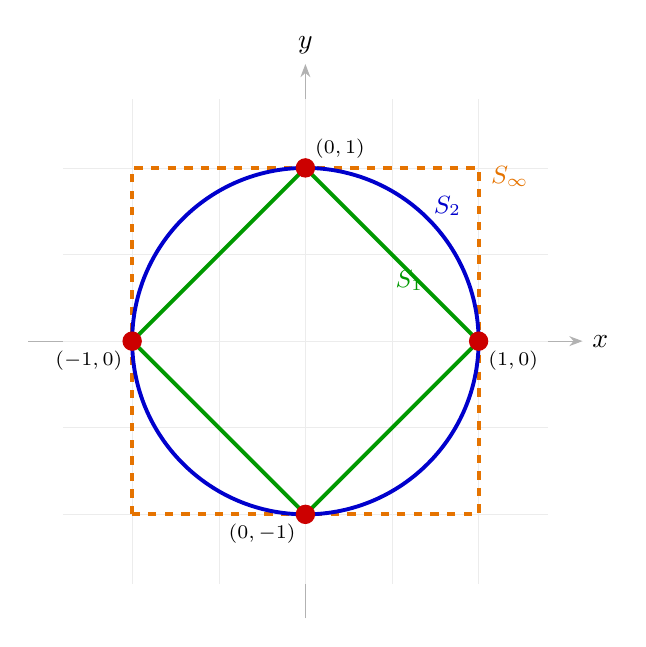
\begin{tikzpicture}[scale=2.2, >=Stealth]
    % Cartesian axes
    \draw[->, gray!60, thin] (-1.6,0) -- (1.6,0) node[right, black] {$x$};
    \draw[->, gray!60, thin] (0,-1.6) -- (0,1.6) node[above, black] {$y$};

    % Light grid
    \draw[step=0.5, gray!15, very thin] (-1.4,-1.4) grid (1.4,1.4);

    % S_infty (Axis-aligned square)
    \draw[line width=1.4pt, orange!90!black, dashed] (-1,-1) rectangle (1,1);
    \node[orange!90!black, font=\small\bfseries] at (1.18, 0.95) {$S_\infty$};

    % S_2 (Circle)
    \draw[line width=1.4pt, blue!80!black] (0,0) circle (1);
    \node[blue!80!black, font=\small\bfseries] at (0.82, 0.78) {$S_2$};

    % S_1 (Rotated diamond)
    \draw[line width=1.4pt, green!60!black] (1,0) -- (0,1) -- (-1,0) -- (0,-1) -- cycle;
    \node[green!60!black, font=\small\bfseries] at (0.6, 0.35) {$S_1$};

    % Common intersection points
    \filldraw[red!80!black] (1,0) circle (1.5pt) node[below right, black, font=\scriptsize] {$(1,0)$};
    \filldraw[red!80!black] (0,1) circle (1.5pt) node[above right, black, font=\scriptsize] {$(0,1)$};
    \filldraw[red!80!black] (-1,0) circle (1.5pt) node[below left, black, font=\scriptsize] {$(-1,0)$};
    \filldraw[red!80!black] (0,-1) circle (1.5pt) node[below left, black, font=\scriptsize] {$(0,-1)$};
\end{tikzpicture}
\caption{Geometric comparison of unit spheres $S_1$ (green diamond), $S_2$ (blue circle), and $S_\infty$ (dashed orange square) in $\R^2$. The four red points mark the intersection $S_1 \cap S_2 \cap S_\infty = \{\pm \mathbf{e}_1, \pm \mathbf{e}_2\}$.}
\label{fig:unit-spheres-en}
\end{figure}

\begin{property}[Common Intersection of Unit Spheres]
The intersection of all three unit loci consists exactly of the canonical basis vectors and their opposites:
\begin{equation}
    S_1 \cap S_2 \cap S_\infty = \left\{ \begin{bmatrix} 1 \\ 0 \end{bmatrix}, \begin{bmatrix} 0 \\ 1 \end{bmatrix}, \begin{bmatrix} -1 \\ 0 \end{bmatrix}, \begin{bmatrix} 0 \\ -1 \end{bmatrix} \right\} = \{\pm \mathbf{e}_1, \pm \mathbf{e}_2\}.
\end{equation}
Only for these four points do all three norms simultaneously evaluate to unity: $\|\mathbf{v}\|_1 = \|\mathbf{v}\|_2 = \|\mathbf{v}\|_\infty = 1$.
\end{property}

\subsection{Exercise 3: Basis Verification in \texorpdfstring{$\R^3$}{R3}}

Consider the three vectors in $\R^3$:
\begin{equation}
    \mathbf{v}_1 = \begin{bmatrix} 1 \\ 0 \\ 2 \end{bmatrix}, \qquad \mathbf{v}_2 = \begin{bmatrix} 2 \\ 2 \\ 0 \end{bmatrix}, \qquad \mathbf{v}_3 = \begin{bmatrix} -3 \\ -4 \\ 2 \end{bmatrix}.
\end{equation}

Testing whether $\mathbf{v}_3$ lies in $\spanop(\mathbf{v}_1, \mathbf{v}_2)$:
\begin{equation}
    \alpha \mathbf{v}_1 + \beta \mathbf{v}_2 = \mathbf{v}_3 \iff \begin{cases}
        \alpha + 2\beta = -3 & \text{(component 1)}, \\
        2\beta = -4 & \text{(component 2)}, \\
        2\alpha = 2 & \text{(component 3)}.
    \end{cases}
\end{equation}
From the third equation, $\alpha = 1$; from the second, $\beta = -2$. Substituting into the first equation:
\begin{equation}
    \alpha + 2\beta = 1 + 2(-2) = 1 - 4 = -3.
\end{equation}
The system is consistent, confirming the non-trivial relation:
\begin{equation}
    \mathbf{v}_1 - 2\mathbf{v}_2 - \mathbf{v}_3 = \mathbf{0}_{\R^3}.
\end{equation}
Thus the vectors are linearly dependent, and $\{\mathbf{v}_1, \mathbf{v}_2, \mathbf{v}_3\}$ \textbf{does not form a basis of $\R^3$}.

\FloatBarrier
\section[Three Perspectives on Matrix-Vector Products]{Three Perspectives on\\ Matrix-Vector Products}

\subsection{Definition and Dimensional Compatibility}

A matrix $A \in \R^{n \times m}$ is an ordered rectangular array with $n$ rows and $m$ columns:
\begin{equation}
    A = \begin{bmatrix}
        A_{11} & A_{12} & \cdots & A_{1m} \\
        A_{21} & A_{22} & \cdots & A_{2m} \\
        \vdots & \vdots & \ddots & \vdots \\
        A_{n1} & A_{n2} & \cdots & A_{nm}
    \end{bmatrix}.
\end{equation}

For the matrix-vector product $\mathbf{c} = A \mathbf{b}$, dimension compatibility requires:
\begin{equation}
    A \in \R^{n \times m}, \quad \mathbf{b} \in \R^{m \times 1} \implies \mathbf{c} = A \mathbf{b} \in \R^{n \times 1}.
\end{equation}
The number of columns in $A$ must equal the length of $\mathbf{b}$.

\subsection{The Three Equivalent Perspectives}

Consider the concrete numerical example:
\begin{equation}
    A = \begin{bmatrix} 2 & 0 & 1 \\ 3 & -1 & 0 \end{bmatrix} \in \R^{2 \times 3}, \qquad \mathbf{b} = \begin{bmatrix} 1 \\ 2 \\ 3 \end{bmatrix} \in \R^3.
\end{equation}

Computational linear algebra examines this product through three complementary lenses:

\paragraph{Perspective 1: Component-Wise Scalar Formula.}
Each entry $c_i$ of the output accumulates along row and column:
\begin{equation}
    c_i = \sum_{j=1}^m A_{ij} b_j \qquad (i = 1, \dots, n).
\end{equation}
In our example:
\begin{align}
    c_1 &= 2 \cdot 1 + 0 \cdot 2 + 1 \cdot 3 = 2 + 0 + 3 = 5, \\
    c_2 &= 3 \cdot 1 + (-1) \cdot 2 + 0 \cdot 3 = 3 - 2 + 0 = 1 \implies \mathbf{c} = \begin{bmatrix} 5 \\ 1 \end{bmatrix}.
\end{align}

\paragraph{Perspective 2: Row Perspective (Inner Products).}
Expressing $A$ by its rows $\mathbf{u}_1^T, \dots, \mathbf{u}_n^T$ with $\mathbf{u}_i \in \R^m$:
\begin{equation}
    A = \begin{bmatrix} \text{---} & \mathbf{u}_1^T & \text{---} \\ \text{---} & \mathbf{u}_2^T & \text{---} \\ & \vdots & \\ \text{---} & \mathbf{u}_n^T & \text{---} \end{bmatrix} \implies c_i = \langle \mathbf{u}_i, \mathbf{b} \rangle = \mathbf{u}_i^T \mathbf{b}.
\end{equation}
Each output component is the Euclidean dot product between the corresponding row of $A$ and vector $\mathbf{b}$.

\paragraph{Perspective 3: Column Perspective (Linear Combinations).}
Expressing $A$ through its $m$ columns $\mathbf{w}_1, \dots, \mathbf{w}_m \in \R^n$:
\begin{equation}
    A = \begin{bmatrix} | & | & & | \\ \mathbf{w}_1 & \mathbf{w}_2 & \dots & \mathbf{w}_m \\ | & | & & | \end{bmatrix} \implies \mathbf{c} = A \mathbf{b} = \sum_{j=1}^m b_j \mathbf{w}_j.
\end{equation}
Output vector $\mathbf{c}$ is a \textbf{linear combination of the columns of $A$} weighted by the scalars of $\mathbf{b}$:
\begin{equation}
    \mathbf{c} = 1 \begin{bmatrix} 2 \\ 3 \end{bmatrix} + 2 \begin{bmatrix} 0 \\ -1 \end{bmatrix} + 3 \begin{bmatrix} 1 \\ 0 \end{bmatrix} = \begin{bmatrix} 2 + 0 + 3 \\ 3 - 2 + 0 \end{bmatrix} = \begin{bmatrix} 5 \\ 1 \end{bmatrix}.
\end{equation}

\begin{noteblock}{Significance of the Column Perspective}
The column perspective is foundational across this course: it reveals that the set of all possible outputs $A \mathbf{b}$ as $\mathbf{b}$ varies is precisely the \textbf{column space} $\mathrm{range}(A) = \spanop(\mathbf{w}_1, \dots, \mathbf{w}_m)$. Solving $A \mathbf{x} = \mathbf{b}$ means finding coefficients $\mathbf{x}$ to reconstruct $\mathbf{b}$ from $A$'s columns.
\end{noteblock}

\FloatBarrier
\section{Matrices as Linear Transformations in the Plane}

A square matrix $A \in \R^{2 \times 2}$ acts on plane vectors as a linear operator $T_A: \R^2 \to \R^2$ defined by $T_A(\mathbf{v}) = A \mathbf{v}$. Its geometric behavior is entirely determined by the images of the standard basis vectors:
\begin{equation}
    A \mathbf{e}_1 = \text{first column of } A, \qquad A \mathbf{e}_2 = \text{second column of } A.
\end{equation}

\subsection{Core Geometric Examples}

\paragraph{1. $90^\circ$ Clockwise Rotation.}
Consider:
\begin{equation}
    A_{\text{rot}} = \begin{bmatrix} 0 & 1 \\ -1 & 0 \end{bmatrix}.
\end{equation}
Acting on the canonical basis:
\begin{equation}
    A_{\text{rot}} \mathbf{e}_1 = \begin{bmatrix} 0 \\ -1 \end{bmatrix} = -\mathbf{e}_2, \qquad A_{\text{rot}} \mathbf{e}_2 = \begin{bmatrix} 1 \\ 0 \end{bmatrix} = \mathbf{e}_1.
\end{equation}
Horizontal vector $\mathbf{e}_1$ rotates downward to $-\mathbf{e}_2$, while vertical vector $\mathbf{e}_2$ rotates rightward to $\mathbf{e}_1$. For general $\mathbf{v} = [v_1, v_2]^T$, it outputs $[v_2, -v_1]^T$, rotating the entire plane by $90^\circ$ clockwise.

\paragraph{2. Horizontal Shear Mapping.}
Consider the upper-triangular matrix:
\begin{equation}
    A_{\text{shear}} = \begin{bmatrix} 1 & 1 \\ 0 & 1 \end{bmatrix}.
\end{equation}
Its action on the basis vectors gives:
\begin{equation}
    A_{\text{shear}} \mathbf{e}_1 = \begin{bmatrix} 1 \\ 0 \end{bmatrix} = \mathbf{e}_1, \qquad A_{\text{shear}} \mathbf{e}_2 = \begin{bmatrix} 1 \\ 1 \end{bmatrix} = \mathbf{e}_1 + \mathbf{e}_2.
\end{equation}
The horizontal axis remains fixed, while the horizontal coordinate shifts proportionally to vertical position ($x \mapsto x + y$, $y \mapsto y$). Squares deform into parallelograms of equal area ($\det A_{\text{shear}} = 1$).

\paragraph{3. Uniform Scaling and Reflection.}
\begin{itemize}
    \item $A = \begin{bmatrix} 2 & 0 \\ 0 & 2 \end{bmatrix} = 2 I$: uniformly dilates every vector by a factor of $2$ ($A \mathbf{v} = 2 \mathbf{v}$), preserving directions and angles.
    \item $A = \begin{bmatrix} 0 & 1 \\ 1 & 0 \end{bmatrix}$: swaps coordinates ($x \mapsto y$, $y \mapsto x$), performing reflection across the line $y = x$.
\end{itemize}

\FloatBarrier
\section{Introduction to Computational Complexity and Flops}

In numerical linear algebra, establishing theoretical solvability is insufficient: one must quantify the required elementary floating-point operations (\textbf{flops} — additions, subtractions, multiplications, divisions).

\subsection{Operation Count for the Inner Product}

For $\mathbf{v}, \mathbf{w} \in \R^n$, computing $\langle \mathbf{v}, \mathbf{w} \rangle = \sum_{i=1}^n v_i w_i$ requires:
\begin{enumerate}
    \item $n$ multiplications ($v_1 w_1, \dots, v_n w_n$);
    \item $n - 1$ additions to sum the partial products.
\end{enumerate}
The exact count is:
\begin{equation}
    \text{Flops}(n) = n + (n - 1) = 2n - 1 \implies \BigO{n}.
\end{equation}

\subsection{Linear Time Scaling Model}

Assuming execution time is proportional to operation count: if computing an inner product of length $n = 10^7$ takes $3$ seconds, tripling the size to $n' = 3 \cdot 10^7$ yields:
\begin{equation}
    \text{Estimated time} = 3 \times (\text{base time}) = 3 \times 3\,\text{s} = 9\,\text{s}.
\end{equation}
Linear complexity $\BigO{n}$ guarantees runtime scales proportionally with dimension.

\begin{remark}[Open Question: The Cost of Matrix-Vector Multiplication]
For a square matrix $A \in \R^{n \times n}$ and vector $\mathbf{b} \in \R^n$:
\begin{itemize}
    \item Evaluating $A \mathbf{b}$ requires computing $n$ independent dot products of length $n$, each costing $2n - 1$:
    \begin{equation}
        \text{Flops}_{\text{mat-vec}}(n) = n (2n - 1) = 2n^2 - n \implies \BigO{n^2}.
    \end{equation}
    \item If computation for $n = 1\,000$ takes $3$ seconds, doubling to $n' = 2\,000$ quadruples the expected time: $(2)^2 \times 3\,\text{s} = 12\,\text{s}$.
\end{itemize}
\end{remark}

\FloatBarrier
\section{Summary of Core Mathematical Concepts}

\begin{table}[H]
  \centering
  \small
  \setlength{\tabcolsep}{5pt}
  \begin{tabularx}{\textwidth}{l Y Y}
    \toprule
    \textbf{Object / Concept} & \textbf{Mathematical Definition} & \textbf{Key Property / Complexity} \\
    \midrule
    $\ell_1$ Norm & $\|\mathbf{v}\|_1 = \sum_{i=1}^n |v_i|$ & Unit sphere is a $45^\circ$ diamond; induces sparsity in models. \\
    $\ell_2$ Norm & $\|\mathbf{v}\|_2 = \sqrt{\sum_{i=1}^n v_i^2} = \sqrt{\mathbf{v}^T \mathbf{v}}$ & Standard rotation-invariant Euclidean length; smooth and differentiable. \\
    $\ell_\infty$ Norm & $\|\mathbf{v}\|_\infty = \max_{1 \le i \le n} |v_i|$ & Unit sphere is an axis-aligned square of side length $2$. \\
    Inner Product & $\langle \mathbf{v}, \mathbf{w} \rangle = \mathbf{v}^T \mathbf{w} = \sum_{i=1}^n v_i w_i$ & Arithmetic operations: $2n - 1 \implies \BigO{n}$. \\
    Basis & Linearly independent set with $\spanop = V$ & Unique coordinate representation for every vector. \\
    Product $A \mathbf{b}$ (Row view) & $c_i = \mathbf{u}_i^T \mathbf{b}$ & $n$ dot products between rows of $A$ and vector $\mathbf{b}$. \\
    Product $A \mathbf{b}$ (Column view) & $\mathbf{c} = \sum_{j=1}^m b_j \mathbf{w}_j$ & Linear combination of columns weighted by $\mathbf{b}$; spans $\mathrm{range}(A)$. \\
    $90^\circ$ Clockwise Rotation & $A = \begin{bmatrix} 0 & 1 \\ -1 & 0 \end{bmatrix}$ & Maps $\mathbf{e}_1 \mapsto -\mathbf{e}_2$ and $\mathbf{e}_2 \mapsto \mathbf{e}_1$. \\
    Reflection across $y = x$ & $A = \begin{bmatrix} 0 & 1 \\ 1 & 0 \end{bmatrix}$ & Maps $\mathbf{e}_1 \mapsto \mathbf{e}_2$ and $\mathbf{e}_2 \mapsto \mathbf{e}_1$, swapping coordinates. \\
    \bottomrule
  \end{tabularx}
  \caption{Summary of algebraic, geometric, and computational concepts covered in Chapter 1.}
  \label{tab:summary-chapter-1-en}
\end{table}

\chapter{Matrix Multiplication, Computational Complexity, and Orthogonal Matrices}
\label{chap:matrix-multiplication-complexity-orthogonality}

This chapter investigates higher-level algebraic operations between matrices, focusing on matrix-matrix multiplication, its computational complexity and scaling laws, and the structural properties of the fundamental subspaces associated with a matrix. We then formalize vector orthogonality and orthogonal matrices, which constitute cornerstone building blocks for designing stable numerical algorithms and canonical matrix factorizations in numerical linear algebra~\cite{trefethen1997numerical}.

\FloatBarrier
\section{Matrix-Matrix Multiplication}

\subsection{Dimensional Compatibility Condition}

Let $A$ and $B$ be real matrices. The matrix product $C = AB$ is well-defined \textbf{if and only if} the number of columns in the first factor $A$ equals the number of rows in the second factor $B$.

\begin{definition}[Dimensional Compatibility of Matrix Products]
Given $n, m, p \in \N$, let $A \in \R^{n \times m}$ and $B \in \R^{m \times p}$. Matrix multiplication produces a matrix $C = AB \in \R^{n \times p}$ whose dimensions match the rows of the first factor and the columns of the second:
\begin{equation}
    A \in \R^{n \times m}, \quad B \in \R^{m \times p} \implies C = AB \in \R^{n \times p}.
\end{equation}
\end{definition}

If the inner dimensions differ, the product is undefined. In general, even for square matrices ($n = m = p$), matrix multiplication is non-commutative:
\begin{equation}
    AB \neq BA \qquad \text{(in general)}.
\end{equation}

\begin{figure}[H]
\centering
\resizebox{0.95\textwidth}{!}{%
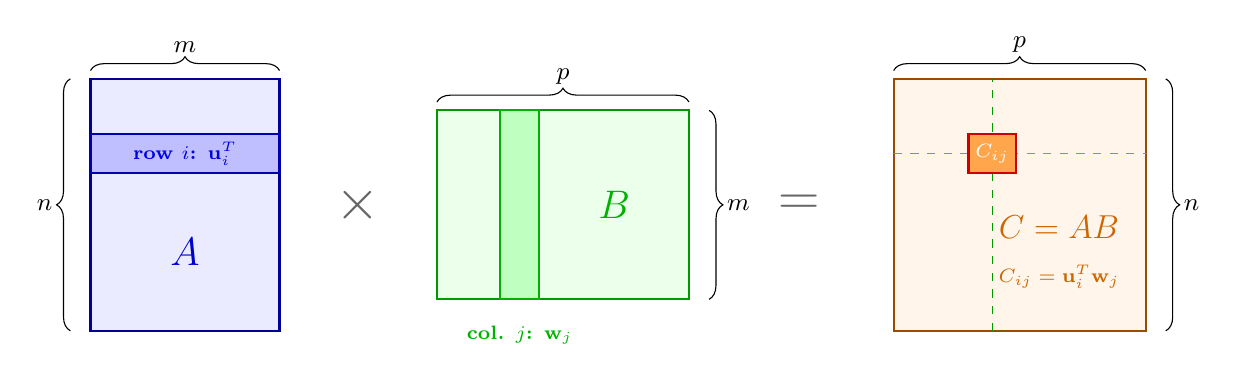
\begin{tikzpicture}[>=Stealth,
    brace/.style={decorate, decoration={brace, amplitude=5pt, raise=3pt}}]
    % --- Matrix A (n x m) ---
    \draw[thick, fill=blue!8, draw=blue!60!black] (0, 0) rectangle (2.4, 3.2);
    % Row i of A highlighted
    \draw[fill=blue!25, draw=blue!70!black, thick] (0, 2.0) rectangle (2.4, 2.5);
    \node[font=\scriptsize\bfseries, text=blue!90!black] at (1.2, 2.25) {row $i$: $\mathbf{u}_i^T$};
    \node[font=\bfseries\Large, text=blue!80!black] at (1.2, 1.0) {$A$};
    % Dimension braces of A (facing outward)
    \draw[brace] (-0.15, 0) -- (-0.15, 3.2) node[midway, left=6pt, font=\small] {$n$};
    \draw[brace] (0, 3.2) -- (2.4, 3.2) node[midway, above=6pt, font=\small] {$m$};

    % Multiplication operator
    \node[font=\huge, text=gray!80!black] at (3.4, 1.6) {$\times$};

    % --- Matrix B (m x p) ---
    \draw[thick, fill=green!8, draw=green!60!black] (4.4, 0.4) rectangle (7.6, 2.8);
    % Column j of B highlighted
    \draw[fill=green!25, draw=green!70!black, thick] (5.2, 0.4) rectangle (5.7, 2.8);
    \node[below=6pt, font=\scriptsize\bfseries, text=green!70!black] at (5.45, 0.4) {col. $j$: $\mathbf{w}_j$};
    \node[font=\bfseries\Large, text=green!70!black] at (6.65, 1.6) {$B$};
    % Dimension braces of B (facing outward)
    \draw[brace] (4.4, 2.8) -- (7.6, 2.8) node[midway, above=6pt, font=\small] {$p$};
    \draw[brace] (7.75, 2.8) -- (7.75, 0.4) node[midway, right=6pt, font=\small] {$m$};

    % Equals operator
    \node[font=\huge, text=gray!80!black] at (9.0, 1.6) {$=$};

    % --- Matrix C (n x p) ---
    \draw[thick, fill=orange!8, draw=orange!60!black] (10.2, 0) rectangle (13.4, 3.2);
    % Dashed guidelines
    \draw[dashed, blue!50, thin] (10.2, 2.25) -- (13.4, 2.25);
    \draw[dashed, green!60!black, thin] (11.45, 0) -- (11.45, 3.2);
    % Entry C_ij at intersection
    \draw[fill=orange!70, draw=red!80!black, thick] (11.15, 2.0) rectangle (11.75, 2.5);
    \node[font=\scriptsize\bfseries, text=white] at (11.45, 2.25) {$C_{ij}$};
    \node[font=\bfseries\large, text=orange!80!black, align=center] at (12.3, 1.0) {$C = AB$\\[2pt]\scriptsize $C_{ij} = \mathbf{u}_i^T \mathbf{w}_j$};
    % Dimension braces of C (facing outward)
    \draw[brace] (10.2, 3.2) -- (13.4, 3.2) node[midway, above=6pt, font=\small] {$p$};
    \draw[brace] (13.55, 3.2) -- (13.55, 0) node[midway, right=6pt, font=\small] {$n$};
\end{tikzpicture}%
}
\caption{Dimensional compatibility in matrix multiplication: entry $C_{ij}$ is formed by the inner product of row $\mathbf{u}_i^T$ of $A$ and column $\mathbf{w}_j$ of $B$.}
\label{fig:matrix-compatibility}
\end{figure}

\subsection{Component-Wise Definition}

Each entry $C_{ij}$ located at row $i$ ($1 \le i \le n$) and column $j$ ($1 \le j \le p$) of the resulting matrix is computed as the standard Euclidean inner product between the $i$-th row of $A$ and the $j$-th column of $B$:

\begin{definition}[Component-Wise Matrix Multiplication Formula]
Given $A \in \R^{n \times m}$ and $B \in \R^{m \times p}$, entry $(i, j)$ of $C = AB$ is:
\begin{equation}
    C_{ij} = \sum_{k=1}^m A_{ik} B_{kj} = A_{i1}B_{1j} + A_{i2}B_{2j} + \dots + A_{im}B_{mj}.
\end{equation}
In vector notation, denoting the $i$-th row of $A$ by $\mathbf{u}_i^T$ and the $j$-th column of $B$ by $\mathbf{w}_j$:
\begin{equation}
    C_{ij} = \langle \mathbf{u}_i, \mathbf{w}_j \rangle = \mathbf{u}_i^T \mathbf{w}_j.
\end{equation}
\end{definition}

\subsection{Step-by-Step Numerical Example}

\begin{example}[Detailed Rectangular Matrix Multiplication]
Consider the matrices:
\begin{equation}
    A = \begin{bmatrix} 1 & 2 \\ 0 & 3 \end{bmatrix} \in \R^{2 \times 2}, \qquad B = \begin{bmatrix} 0 & 1 & -1 \\ 1 & 0 & 2 \end{bmatrix} \in \R^{2 \times 3}.
\end{equation}
Since $A$ has $m = 2$ columns and $B$ has $m = 2$ rows, product $C = AB$ is well-defined and yields a $2 \times 3$ matrix. We compute each component analytically:

\paragraph{First row of $C$ (row 1 of $A$ against columns of $B$):}
\begin{align}
    C_{11} &= A_{11}B_{11} + A_{12}B_{21} = 1 \cdot 0 + 2 \cdot 1 = 0 + 2 = 2, \\
    C_{12} &= A_{11}B_{12} + A_{12}B_{22} = 1 \cdot 1 + 2 \cdot 0 = 1 + 0 = 1, \\
    C_{13} &= A_{11}B_{13} + A_{12}B_{23} = 1 \cdot (-1) + 2 \cdot 2 = -1 + 4 = 3.
\end{align}

\paragraph{Second row of $C$ (row 2 of $A$ against columns of $B$):}
\begin{align}
    C_{21} &= A_{21}B_{11} + A_{22}B_{21} = 0 \cdot 0 + 3 \cdot 1 = 0 + 3 = 3, \\
    C_{22} &= A_{21}B_{12} + A_{22}B_{22} = 0 \cdot 1 + 3 \cdot 0 = 0 + 0 = 0, \\
    C_{23} &= A_{21}B_{13} + A_{22}B_{23} = 0 \cdot (-1) + 3 \cdot 2 = 0 + 6 = 6.
\end{align}

Assembling the calculated components yields:
\begin{equation}
    C = AB = \begin{bmatrix} 2 & 1 & 3 \\ 3 & 0 & 6 \end{bmatrix} \in \R^{2 \times 3}.
\end{equation}
\end{example}

\FloatBarrier
\section{Computational Complexity and Scaling Law}

\subsection{Rigorous FLOP Counting}

Assessing numerical algorithm execution time requires quantifying floating-point operations (FLOPs).

\begin{property}[Computational Cost of Matrix Multiplication]
\mbox{}\par\nopagebreak
\begin{enumerate}
    \item \textbf{Cost of a single entry:}
    Evaluating $C_{ij} = \sum_{k=1}^m A_{ik} B_{kj}$ requires $m$ scalar multiplications and $m - 1$ additions:
    \begin{equation}
        \text{FLOPs per entry} = m + (m - 1) = 2m - 1 \quad \implies \quad \BigO{m}.
    \end{equation}
    \item \textbf{General rectangular case ($A \in \R^{n \times m}, B \in \R^{m \times p}$):}
    Computing all $n \cdot p$ independent entries yields:
    \begin{equation}
        \text{Total FLOPs} = n \cdot p \cdot (2m - 1) = 2nmp - np \quad \implies \quad \BigO{nmp}.
    \end{equation}
    \item \textbf{Square matrix case ($n = m = p$):}
    When both matrices belong to $\R^{n \times n}$, matrix $C$ has $n^2$ entries:
    \begin{equation}
        \text{Total FLOPs}(n) = n^2 \cdot (2n - 1) = 2n^3 - n^2 \quad \implies \quad \BigO{n^3}.
    \end{equation}
\end{enumerate}
\end{property}

The leading term $2n^3$ dictates cubic growth with respect to dimension $n$.

\subsection{Cubic Time Scaling Law}

Let $T(n) \approx \gamma n^3$ model execution time on fixed hardware, where $\gamma > 0$ absorbs cache architecture, CPU clock speed, and compiler optimization.

\begin{example}[Predicting Execution Time under Doubled Dimension]
Suppose multiplying two dense square matrices of size $n = 1000$ takes $3\text{ seconds}$ of CPU time:
\begin{equation}
    T(1000) \approx \gamma \cdot (1000)^3 = 3\text{ s}.
\end{equation}
Doubling the dimension to $n' = 2000$, the cubic scaling law implies:
\begin{equation}
    T(2000) \approx \gamma \cdot (2000)^3 = \gamma \cdot (2 \cdot 1000)^3 = 8 \cdot \left(\gamma \cdot 1000^3\right) = 8 \cdot T(1000).
\end{equation}
The execution time scales by a factor of $8$:
\begin{equation}
    T(2000) \approx 8 \cdot 3\text{ s} = 24\text{ seconds}.
\end{equation}
\end{example}

\subsection{Comparative Overview of Core Linear Algebra Operations}

Table~\ref{tab:complexity-comparison} illustrates how the three foundational linear algebra operations scale when the linear data dimension $n$ increases by a factor of $10$ (from $n = 10^3$ to $n = 10^4$).

\begin{table}[H]
\centering
\resizebox{0.95\textwidth}{!}{%
\begin{tabular}{l l c l c}
\toprule
\textbf{Operation} & \textbf{Operands} & \textbf{FLOP Formula} & \textbf{Cost} & \textbf{Scaling Factor ($10\times$)} \\
\midrule
Inner Product & $\mathbf{v}, \mathbf{w} \in \R^n$ & $2n - 1$ & $\BigO{n}$ & $10^1 = 10$ \\
Matrix-Vector & $A \in \R^{n \times n}, \mathbf{b} \in \R^n$ & $2n^2 - n$ & $\BigO{n^2}$ & $10^2 = 100$ \\
Matrix-Matrix & $A, B \in \R^{n \times n}$ & $2n^3 - n^2$ & $\BigO{n^3}$ & $10^3 = 1000$ \\
\bottomrule
\end{tabular}%
}
\caption{Complexity comparison and scaling factors for a tenfold increase in dimension.}
\label{tab:complexity-comparison}
\end{table}

If an $n = 1000$ matrix-matrix multiplication runs in $1\text{ second}$, the same task for $n = 10\,000$ requires $1000\text{ seconds}$ ($\approx 16.6\text{ minutes}$).

\FloatBarrier
\section[Fundamental Properties: Rank, Subspaces, and Invertibility]{Fundamental Properties: Rank,\\ Subspaces, and Invertibility}

\subsection{Subspaces Associated with a Linear Map}

Let $A \in \R^{n \times m}$ define a linear operator $T_A: \R^m \to \R^n$ via $T_A(\mathbf{x}) = A\mathbf{x}$.

\begin{definition}[Rank of a Matrix]
The \textbf{rank} of $A$, denoted by $\rank(A)$, is the dimension of the vector space spanned by its columns. By the fundamental theorem of linear algebra, column rank and row rank always coincide:
\begin{equation}
    \rank(A) = \dim(\mathrm{col}(A)) = \dim(\mathrm{row}(A)) \le \min(n, m).
\end{equation}
When $\rank(A) = \min(n, m)$, the matrix is said to have \textbf{full rank}.
\end{definition}

\begin{definition}[Kernel or Nullspace]
The \textbf{kernel} (or \textit{nullspace}) of $A$ is the subspace of $\R^m$ containing all vectors mapped to the zero vector in $\R^n$:
\begin{equation}
    \ker(A) = \left\{ \mathbf{x} \in \R^m : A\mathbf{x} = \mathbf{0}_{\R^n} \right\} \subseteq \R^m.
\end{equation}
\end{definition}

\begin{definition}[Image or Range]
The \textbf{image} (or \textit{range}) of $A$ is the subspace of $\R^n$ spanned by all linear combinations of the columns of $A$:
\begin{equation}
    \mathrm{Im}(A) = \spanop(\text{columns of } A) = \left\{ A\mathbf{x} : \mathbf{x} \in \R^m \right\} \subseteq \R^n.
\end{equation}
We have $\dim(\mathrm{Im}(A)) = \rank(A)$.
\end{definition}

\begin{theorem}[Rank-Nullity Theorem]
For any matrix $A \in \R^{n \times m}$ with $m$ columns, the dimension of the image plus the dimension of the kernel equals the dimension of the domain:
\begin{equation}
    \dim(\mathrm{Im}(A)) + \dim(\ker(A)) = m.
\end{equation}
\end{theorem}

\begin{figure}[H]
\centering
\resizebox{0.92\textwidth}{!}{%
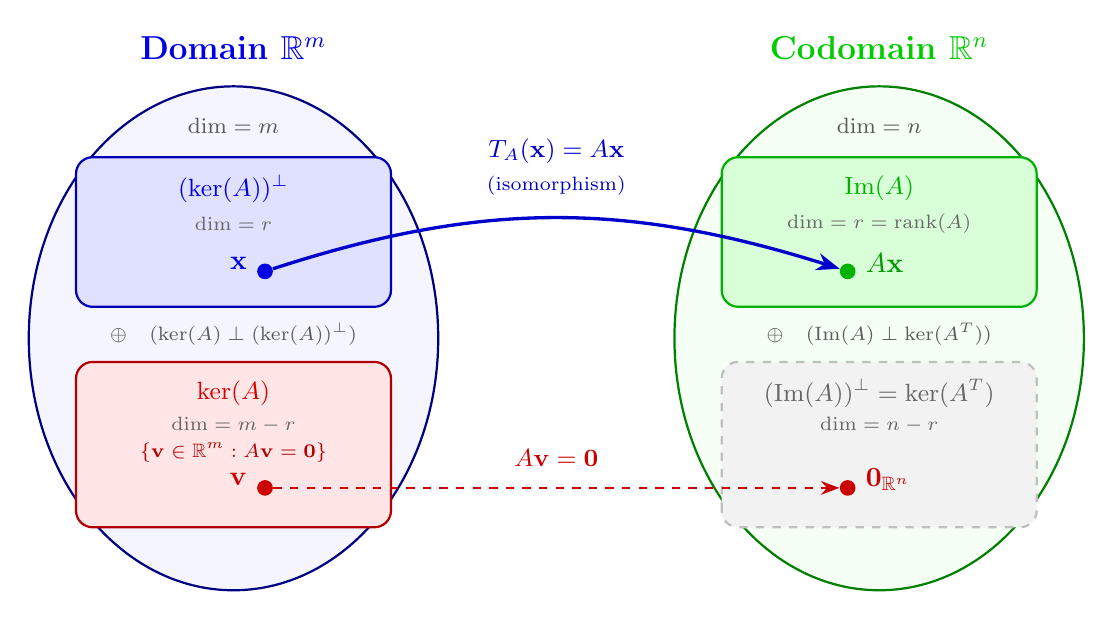
\begin{tikzpicture}[>=Stealth,
    subspace/.style={thick, rounded corners=6pt},
    point/.style={circle, fill, inner sep=2pt}]

    % ================= DOMAIN R^m =================
    \draw[thick, fill=blue!4, draw=blue!50!black] (0, 0) ellipse (2.6 and 3.2);
    \node[above=6pt, font=\bfseries\large, text=blue!90!black] at (0, 3.2) {Domain $\R^m$};
    \node[font=\footnotesize, text=gray!70!black] at (0, 2.7) {$\dim = m$};

    % Orthogonal subspace (ker A)^\perp
    \draw[subspace, fill=blue!12, draw=blue!70!black] (-2.0, 0.4) rectangle (2.0, 2.3);
    \node[font=\small\bfseries, text=blue!90!black] at (0, 1.9) {$(\ker(A))^\perp$};
    \node[font=\scriptsize, text=gray!80!black] at (0, 1.45) {$\dim = r$};
    \node[point, fill=blue!90!black, label={[blue!90!black, left=3pt]:$\mathbf{x}$}] (x) at (0.4, 0.85) {};

    % Internal direct sum symbol
    \node[font=\scriptsize, text=gray!70!black] at (0, 0.05) {$\oplus \quad (\ker(A) \perp (\ker(A))^\perp)$};

    % Kernel ker(A)
    \draw[subspace, fill=red!10, draw=red!70!black] (-2.0, -2.4) rectangle (2.0, -0.3);
    \node[font=\small\bfseries, text=red!85!black] at (0, -0.7) {$\ker(A)$};
    \node[font=\scriptsize, text=gray!80!black] at (0, -1.1) {$\dim = m - r$};
    \node[font=\scriptsize, text=red!70!black] at (0, -1.45) {$\{ \mathbf{v} \in \R^m : A\mathbf{v} = \mathbf{0} \}$};
    \node[point, fill=red!80!black, label={[red!80!black, left=3pt]:$\mathbf{v}$}] (v) at (0.4, -1.9) {};

    % ================= CODOMAIN R^n =================
    \begin{scope}[xshift=8.2cm]
        \draw[thick, fill=green!4, draw=green!50!black] (0, 0) ellipse (2.6 and 3.2);
        \node[above=6pt, font=\bfseries\large, text=green!80!black] at (0, 3.2) {Codomain $\R^n$};
        \node[font=\footnotesize, text=gray!70!black] at (0, 2.7) {$\dim = n$};

        % Image Im(A)
        \draw[subspace, fill=green!15, draw=green!70!black] (-2.0, 0.4) rectangle (2.0, 2.3);
        \node[font=\small\bfseries, text=green!70!black] at (0, 1.9) {$\mathrm{Im}(A)$};
        \node[font=\scriptsize, text=gray!80!black] at (0, 1.45) {$\dim = r = \rank(A)$};
        \node[point, fill=green!70!black, label={[green!60!black, right=3pt]:$A\mathbf{x}$}] (Ax) at (-0.4, 0.85) {};

        % Internal direct sum symbol
        \node[font=\scriptsize, text=gray!70!black] at (0, 0.05) {$\oplus \quad (\mathrm{Im}(A) \perp \ker(A^T))$};

        % Complement / ker(A^T)
        \draw[subspace, fill=gray!10, draw=gray!50, dashed] (-2.0, -2.4) rectangle (2.0, -0.3);
        \node[font=\small\bfseries, text=gray!80!black] at (0, -0.7) {$(\mathrm{Im}(A))^\perp = \ker(A^T)$};
        \node[font=\scriptsize, text=gray!80!black] at (0, -1.1) {$\dim = n - r$};
        \node[point, fill=red!80!black, label={[red!80!black, right=3pt]:$\mathbf{0}_{\R^n}$}] (zero) at (-0.4, -1.9) {};
    \end{scope}

    % ================= MAPS / TRANSFORMATIONS =================
    % Isomorphism mapping from complement to Im(A)
    \draw[->, very thick, blue!80!black] (x) to[out=18, in=162] node[midway, above=4pt, font=\small, align=center] {$T_A(\mathbf{x}) = A\mathbf{x}$\\[1pt]\scriptsize (isomorphism)} (Ax);

    % Kernel mapping to zero
    \draw[->, thick, dashed, red!80!black] (v) -- node[midway, above=4pt, font=\small] {$A\mathbf{v} = \mathbf{0}$} (zero);

\end{tikzpicture}%
}
\caption{Geometric representation of fundamental subspaces and the Rank-Nullity Theorem: $\dim(\ker(A)) + \dim(\mathrm{Im}(A)) = m$. The restriction of $A$ to the orthogonal complement $(\ker(A))^\perp$ is an isomorphism onto $\mathrm{Im}(A)$.}
\label{fig:fundamental-subspaces}
\end{figure}

\subsection{Invertibility of Square Matrices}

For square matrices $A \in \R^{n \times n}$, rank, nullity, and invertibility merge into an overarching equivalence theorem.

\begin{definition}[Invertible or Non-Singular Matrix]
A matrix $A \in \R^{n \times n}$ is called \textbf{invertible} if there exists a unique matrix $A^{-1} \in \R^{n \times n}$ satisfying:
\begin{equation}
    A A^{-1} = I_n \qquad \text{and} \qquad A^{-1} A = I_n.
\end{equation}
\end{definition}

\begin{theorem}[Equivalent Characterizations of Invertibility]
Let $A \in \R^{n \times n}$. The following statements are equivalent:
\mbox{}\par\nopagebreak
\begin{enumerate}
    \item $A$ is invertible.
    \item $\rank(A) = n$ ($A$ has full rank).
    \item $\det(A) \neq 0$.
    \item $\ker(A) = \{ \mathbf{0}_{\R^n} \}$ (trivial nullspace).
    \item The columns of $A$ form a basis of $\R^n$.
    \item Linear system $A\mathbf{x} = \mathbf{b}$ has a unique solution $\mathbf{x} = A^{-1}\mathbf{b}$ for every $\mathbf{b} \in \R^n$.
\end{enumerate}
\end{theorem}

\subsection{Guided Example: Rank, Kernel, and Image Calculation}

\begin{example}[Full Subspace Analysis of a Singular $3 \times 3$ Matrix]
Consider the matrix:
\begin{equation}
    A = \begin{bmatrix} 1 & 2 & 0 \\ 2 & 4 & 0 \\ 0 & 0 & 1 \end{bmatrix} \in \R^{3 \times 3}.
\end{equation}

\paragraph{1. Rank via Gaussian Elimination:}
Apply elementary row operation $R_2 \leftarrow R_2 - 2R_1$:
\begin{equation}
    \begin{bmatrix} 1 & 2 & 0 \\ 2 & 4 & 0 \\ 0 & 0 & 1 \end{bmatrix}
    \xrightarrow{R_2 \to R_2 - 2R_1}
    \begin{bmatrix} 1 & 2 & 0 \\ 0 & 0 & 0 \\ 0 & 0 & 1 \end{bmatrix}
    \xrightarrow{R_2 \leftrightarrow R_3}
    \begin{bmatrix} 1 & 2 & 0 \\ 0 & 0 & 1 \\ 0 & 0 & 0 \end{bmatrix}.
\end{equation}
The row echelon form contains 2 non-zero pivots. Therefore:
\begin{equation}
    \rank(A) = 2.
\end{equation}
Since $\rank(A) = 2 < 3$, matrix $A$ is \textbf{not invertible} ($\det(A) = 0$).

\paragraph{2. Image Space $\mathrm{Im}(A)$:}
Examining the columns of $A$:
\begin{equation}
    \mathbf{a}_1 = \begin{bmatrix} 1 \\ 2 \\ 0 \end{bmatrix}, \qquad \mathbf{a}_2 = \begin{bmatrix} 2 \\ 4 \\ 0 \end{bmatrix} = 2\mathbf{a}_1, \qquad \mathbf{a}_3 = \begin{bmatrix} 0 \\ 0 \\ 1 \end{bmatrix}.
\end{equation}
The second column is collinear to the first and hence redundant. Columns $\mathbf{a}_1$ and $\mathbf{a}_3$ are linearly independent and form a basis for the image:
\begin{equation}
    \mathrm{Im}(A) = \spanop\left\{ \begin{bmatrix} 1 \\ 2 \\ 0 \end{bmatrix}, \begin{bmatrix} 0 \\ 0 \\ 1 \end{bmatrix} \right\}, \qquad \dim(\mathrm{Im}(A)) = 2.
\end{equation}

\paragraph{3. Kernel Space $\ker(A)$:}
Solve homogeneous linear system $A\mathbf{x} = \mathbf{0}_{\R^3}$ with $\mathbf{x} = [x_1, x_2, x_3]^T$:
\begin{equation}
    \begin{bmatrix} 1 & 2 & 0 \\ 2 & 4 & 0 \\ 0 & 0 & 1 \end{bmatrix} \begin{bmatrix} x_1 \\ x_2 \\ x_3 \end{bmatrix} = \begin{bmatrix} 0 \\ 0 \\ 0 \end{bmatrix} \implies \begin{cases} x_1 + 2x_2 = 0 \\ x_3 = 0 \end{cases} \implies \begin{cases} x_1 = -2x_2 \\ x_3 = 0 \end{cases}.
\end{equation}
Setting free variable $x_2 = t \in \R$:
\begin{equation}
    \mathbf{x} = \begin{bmatrix} -2t \\ t \\ 0 \end{bmatrix} = t \begin{bmatrix} -2 \\ 1 \\ 0 \end{bmatrix} \implies \ker(A) = \spanop\left\{ \begin{bmatrix} -2 \\ 1 \\ 0 \end{bmatrix} \right\}.
\end{equation}
The nullity is $\dim(\ker(A)) = 1$. Verifying the Rank-Nullity Theorem:
\begin{equation}
    \dim(\mathrm{Im}(A)) + \dim(\ker(A)) = 2 + 1 = 3 = m.
\end{equation}
\end{example}

\FloatBarrier
\section{Vector Orthogonality and Orthonormality}

\subsection{Core Definitions}

\begin{definition}[Orthogonal Vectors]
Two vectors $\mathbf{v}, \mathbf{w} \in \R^n$ are \textbf{orthogonal} ($\mathbf{v} \perp \mathbf{w}$) if and only if their standard dot product vanishes:
\begin{equation}
    \langle \mathbf{v}, \mathbf{w} \rangle = \mathbf{v}^T \mathbf{w} = 0.
\end{equation}
\end{definition}

\begin{definition}[Orthogonal and Orthonormal Sets]
A set of vectors $\{\mathbf{v}_1, \dots, \mathbf{v}_k\} \subset \R^n$ is called:
\mbox{}\par\nopagebreak
\begin{enumerate}
    \item \textbf{Orthogonal} if vectors are mutually perpendicular:
    \begin{equation}
        \langle \mathbf{v}_i, \mathbf{v}_j \rangle = 0 \qquad \forall i \neq j.
    \end{equation}
    \item \textbf{Orthonormal} if it is orthogonal and every vector has unit Euclidean norm:
    \begin{equation}
        \langle \mathbf{v}_i, \mathbf{v}_j \rangle = \delta_{ij} = \begin{cases} 1 & \text{if } i = j, \\ 0 & \text{if } i \neq j, \end{cases}
    \end{equation}
    where $\delta_{ij}$ is the Kronecker delta.
\end{enumerate}
\end{definition}

\subsection{Constructive Normalization Exercises in \texorpdfstring{$\R^2$}{R2}}

\begin{example}[Constructing and Normalizing an Orthogonal Pair]
\mbox{}\par\nopagebreak
\begin{enumerate}
    \item \textbf{Finding an orthogonal vector:}
    Given vector $\mathbf{v}_1 = [2, 1]^T \in \R^2$, find a non-zero vector $\mathbf{v}_2 = [x, y]^T$ such that $\langle \mathbf{v}_1, \mathbf{v}_2 \rangle = 0$:
    \begin{equation}
        2x + y = 0 \implies y = -2x.
    \end{equation}
    Choosing $x = 1$ yields $y = -2$, producing the orthogonal pair:
    \begin{equation}
        \mathbf{v}_1 = \begin{bmatrix} 2 \\ 1 \end{bmatrix}, \qquad \mathbf{v}_2 = \begin{bmatrix} 1 \\ -2 \end{bmatrix}, \qquad \langle \mathbf{v}_1, \mathbf{v}_2 \rangle = 2(1) + 1(-2) = 0.
    \end{equation}
    \item \textbf{Euclidean Normalization (Orthonormalization):}
    Dividing each vector by its Euclidean $\ell_2$ norm:
    \begin{align}
        \|\mathbf{v}_1\|_2 &= \sqrt{2^2 + 1^2} = \sqrt{5} \implies \mathbf{u}_1 = \frac{\mathbf{v}_1}{\|\mathbf{v}_1\|_2} = \begin{bmatrix} 2/\sqrt{5} \\ 1/\sqrt{5} \end{bmatrix}, \\
        \|\mathbf{v}_2\|_2 &= \sqrt{1^2 + (-2)^2} = \sqrt{5} \implies \mathbf{u}_2 = \frac{\mathbf{v}_2}{\|\mathbf{v}_2\|_2} = \begin{bmatrix} 1/\sqrt{5} \\ -2/\sqrt{5} \end{bmatrix}.
    \end{align}
    Verifying orthonormality:
    \begin{align}
        \|\mathbf{u}_1\|_2 &= 1, \qquad \|\mathbf{u}_2\|_2 = 1, \\
        \langle \mathbf{u}_1, \mathbf{u}_2 \rangle &= \frac{2}{\sqrt{5}}\frac{1}{\sqrt{5}} + \frac{1}{\sqrt{5}}\left(-\frac{2}{\sqrt{5}}\right) = \frac{2}{5} - \frac{2}{5} = 0.
    \end{align}
    The set $\{\mathbf{u}_1, \mathbf{u}_2\}$ forms an orthonormal basis of $\R^2$.
\end{enumerate}
\end{example}

\FloatBarrier
\section{Orthogonal Matrices}

\subsection{Definition and Transpose Properties}

Recall that for general matrix $A \in \R^{n \times m}$, the transpose $A^T \in \R^{m \times n}$ has entries $(A^T)_{ij} = A_{ji}$. For any compatible matrices, the transpose of a product reverses order:
\begin{equation}
    (AB)^T = B^T A^T.
\end{equation}

\begin{definition}[Orthogonal Matrix]
A square matrix $U \in \R^{n \times n}$ is \textbf{orthogonal} if and only if its transpose equals its inverse:
\begin{equation}
    U^T U = U U^T = I_n \iff U^{-1} = U^T.
\end{equation}
\end{definition}

\subsection{Column and Row Characterization}

\begin{theorem}[Column and Row Orthonormality]
A square matrix $U \in \R^{n \times n}$ is orthogonal if and only if its columns form an orthonormal basis of $\R^n$. Equivalently, $U$ is orthogonal if and only if its rows form an orthonormal basis of $\R^n$.
\end{theorem}

\begin{proof}
Partition $U$ into column vectors $\mathbf{u}_1, \mathbf{u}_2, \dots, \mathbf{u}_n \in \R^n$:
\begin{equation}
    U = \begin{bmatrix} \mathbf{u}_1 & \mathbf{u}_2 & \dots & \mathbf{u}_n \end{bmatrix}.
\end{equation}
Then $U^T$ is partitioned by rows:
\begin{equation}
    U^T = \begin{bmatrix} \mathbf{u}_1^T \\ \mathbf{u}_2^T \\ \vdots \\ \mathbf{u}_n^T \end{bmatrix}.
\end{equation}
Computing block matrix product $U^T U$:
\begin{align}
    U^T U &= \begin{bmatrix} \mathbf{u}_1^T \\ \mathbf{u}_2^T \\ \vdots \\ \mathbf{u}_n^T \end{bmatrix} \begin{bmatrix} \mathbf{u}_1 & \mathbf{u}_2 & \dots & \mathbf{u}_n \end{bmatrix} \nonumber \\
    &= \begin{bmatrix}
        \mathbf{u}_1^T \mathbf{u}_1 & \mathbf{u}_1^T \mathbf{u}_2 & \cdots & \mathbf{u}_1^T \mathbf{u}_n \\
        \mathbf{u}_2^T \mathbf{u}_1 & \mathbf{u}_2^T \mathbf{u}_2 & \cdots & \mathbf{u}_2^T \mathbf{u}_n \\
        \vdots & \vdots & \ddots & \vdots \\
        \mathbf{u}_n^T \mathbf{u}_1 & \mathbf{u}_n^T \mathbf{u}_2 & \cdots & \mathbf{u}_n^T \mathbf{u}_n
    \end{bmatrix} = \left[ \langle \mathbf{u}_i, \mathbf{u}_j \rangle \right]_{i,j=1}^n.
\end{align}
For this product to equal identity matrix $I_n$, we must have:
\begin{equation}
    \langle \mathbf{u}_i, \mathbf{u}_j \rangle = \delta_{ij} \qquad \forall i, j \in \{1, \dots, n\}.
\end{equation}
Thus the columns are mutually orthogonal and have unit Euclidean norm. The identical reasoning applied to $U U^T = I_n$ proves that rows are orthonormal.
\end{proof}

\subsection{Prototypical Example: Planar Rotation Matrix}

\begin{example}[Planar Rotation Matrix]
Let $\theta \in \R$. Consider clockwise rotation matrix:
\begin{equation}
    U = \begin{bmatrix} \cos\theta & \sin\theta \\ -\sin\theta & \cos\theta \end{bmatrix}.
\end{equation}
Verifying $U^T U = I_2$:
\begin{align}
    U^T U &= \begin{bmatrix} \cos\theta & -\sin\theta \\ \sin\theta & \cos\theta \end{bmatrix} \begin{bmatrix} \cos\theta & \sin\theta \\ -\sin\theta & \cos\theta \end{bmatrix} \nonumber \\
    &= \begin{bmatrix}
        \cos^2\theta + \sin^2\theta & \cos\theta\sin\theta - \sin\theta\cos\theta \\
        \sin\theta\cos\theta - \cos\theta\sin\theta & \sin^2\theta + \cos^2\theta
    \end{bmatrix} = \begin{bmatrix} 1 & 0 \\ 0 & 1 \end{bmatrix} = I_2.
\end{align}
Matrix $U$ is orthogonal for all angles $\theta$.
\end{example}

\subsection{Closure under Matrix Products}

\begin{proposition}[Orthogonal Group and Product Closure]
If $U, V \in \R^{n \times n}$ are orthogonal matrices, their product $Q = UV$ is also orthogonal.
\end{proposition}

\begin{proof}
Compute $Q Q^T$ using the reversal rule $(UV)^T = V^T U^T$:
\begin{equation}
    Q Q^T = (UV)(UV)^T = (UV)(V^T U^T).
\end{equation}
By associativity of matrix products:
\begin{equation}
    Q Q^T = U (V V^T) U^T.
\end{equation}
Since $V$ is orthogonal, $V V^T = I_n$:
\begin{equation}
    Q Q^T = U I_n U^T = U U^T = I_n.
\end{equation}
Similarly, $Q^T Q = V^T (U^T U) V = V^T I_n V = I_n$. Hence $Q = UV$ is orthogonal.
\end{proof}

\FloatBarrier
\section{The Four Noteworthy Questions on Orthogonal Matrices}

\subsection{Question 1: Upper Bound on Individual Matrix Entries}

\begin{example}[Can an Orthogonal Matrix Entry Exceed 1?]
\textbf{Question:} Can an orthogonal matrix $U \in \R^{n \times n}$ have an entry $U_{ij} > 1$?

\textbf{Answer: NO.} \\
\textbf{Proof:} Let $\mathbf{u}_j$ denote the $j$-th column of $U$. Since $U$ is orthogonal, $\mathbf{u}_j$ has unit Euclidean norm:
\begin{equation}
    \|\mathbf{u}_j\|_2^2 = \sum_{k=1}^n U_{kj}^2 = 1.
\end{equation}
Since each squared entry $U_{kj}^2 \ge 0$, every single term is bounded by the total sum:
\begin{equation}
    U_{ij}^2 \le \sum_{k=1}^n U_{kj}^2 = 1 \implies |U_{ij}| \le 1 \implies -1 \le U_{ij} \le 1.
\end{equation}
No entry of an orthogonal matrix can exceed $1$ in absolute value.
\end{example}

\subsection{Question 2: Orthogonal Diagonal Matrices}

\begin{example}[Characterizing Orthogonal Diagonal Matrices]
\textbf{Question:} When is a diagonal matrix $D \in \R^{n \times n}$ orthogonal?

\textbf{Solution:} Let $D = \diag(d_1, d_2, \dots, d_n)$. Being diagonal, $D^T = D$. Computing $D^T D$:
\begin{equation}
    D^T D = D^2 = \diag(d_1^2, d_2^2, \dots, d_n^2).
\end{equation}
For $D^T D = I_n$, each diagonal entry must satisfy:
\begin{equation}
    d_i^2 = 1 \iff d_i = \pm 1 \qquad \forall i = 1, \dots, n.
\end{equation}
\textbf{Conclusion:} A diagonal matrix is orthogonal if and only if all diagonal entries are $+1$ or $-1$. There exist exactly $2^n$ distinct orthogonal diagonal matrices in $\R^{n \times n}$.
\end{example}

\subsection{Question 3: Orthogonal Upper Triangular Matrices}

\begin{example}[Characterizing Orthogonal Upper Triangular Matrices]
\textbf{Question:} When is an upper triangular matrix $R \in \R^{n \times n}$ orthogonal?

\textbf{Proof by column induction:} Let $R$ be upper triangular ($R_{ij} = 0$ for all $i > j$):
\begin{equation}
    R = \begin{bmatrix}
        r_{11} & r_{12} & r_{13} & \cdots & r_{1n} \\
        0 & r_{22} & r_{23} & \cdots & r_{2n} \\
        0 & 0 & r_{33} & \cdots & r_{3n} \\
        \vdots & \vdots & \vdots & \ddots & \vdots \\
        0 & 0 & 0 & \cdots & r_{nn}
    \end{bmatrix}.
\end{equation}
Since $R$ is orthogonal, its columns $\mathbf{r}_1, \dots, \mathbf{r}_n$ must form an orthonormal basis:
\begin{enumerate}
    \item \textbf{First column $\mathbf{r}_1 = [r_{11}, 0, \dots, 0]^T$:}
    Unit norm requires $r_{11}^2 = 1 \implies r_{11} = \pm 1$.
    \item \textbf{Second column $\mathbf{r}_2 = [r_{12}, r_{22}, 0, \dots, 0]^T$:}
    Orthogonality to $\mathbf{r}_1$ requires:
    \begin{equation}
        \langle \mathbf{r}_1, \mathbf{r}_2 \rangle = r_{11} r_{12} = 0 \implies r_{12} = 0 \quad (\text{since } r_{11} = \pm 1 \neq 0).
    \end{equation}
    Unit norm gives $\|\mathbf{r}_2\|_2^2 = r_{12}^2 + r_{22}^2 = 0 + r_{22}^2 = 1 \implies r_{22} = \pm 1$.
    \item \textbf{Third column $\mathbf{r}_3 = [r_{13}, r_{23}, r_{33}, 0, \dots, 0]^T$:}
    Orthogonality to $\mathbf{r}_1$ and $\mathbf{r}_2$ forces $r_{11} r_{13} = 0 \implies r_{13} = 0$ and $r_{22} r_{23} = 0 \implies r_{23} = 0$. Hence $r_{33} = \pm 1$.
    \item \textbf{Inductive step:} For every column $j$, all off-diagonal entries vanish ($r_{ij} = 0$ for $i < j$), and diagonal entries satisfy $r_{jj} = \pm 1$.
\end{enumerate}
\textbf{Conclusion:} An upper triangular matrix is orthogonal if and only if it is diagonal with diagonal entries $\pm 1$.
\end{example}

\subsection{Question 4: Euclidean Isometry and Norm Preservation}

\begin{theorem}[Isometry Property of Orthogonal Matrices]
\label{thm:en:orthogonal-isometry}
Orthogonal matrices strictly preserve Euclidean vector lengths and standard inner products:
\begin{equation}
    \forall U \in \R^{n \times n} \text{ orthogonal}, \quad \forall \mathbf{x} \in \R^n \implies \|U\mathbf{x}\|_2 = \|\mathbf{x}\|_2.
\end{equation}
Furthermore, inner products between arbitrary pairs of vectors are preserved:
\begin{equation}
    \langle U\mathbf{x}, U\mathbf{y} \rangle = \langle \mathbf{x}, \mathbf{y} \rangle \qquad \forall \mathbf{x}, \mathbf{y} \in \R^n.
\end{equation}
\end{theorem}

\begin{proof}
Recall that for any vector $\mathbf{v}$, $\|\mathbf{v}\|_2^2 = \mathbf{v}^T \mathbf{v}$. Setting $\mathbf{v} = U\mathbf{x}$:
\begin{equation}
    \|U\mathbf{x}\|_2^2 = (U\mathbf{x})^T (U\mathbf{x}).
\end{equation}
Applying the transpose product rule $(U\mathbf{x})^T = \mathbf{x}^T U^T$:
\begin{equation}
    \|U\mathbf{x}\|_2^2 = \mathbf{x}^T (U^T U) \mathbf{x}.
\end{equation}
Since $U$ is orthogonal, $U^T U = I_n$:
\begin{equation}
    \|U\mathbf{x}\|_2^2 = \mathbf{x}^T I_n \mathbf{x} = \mathbf{x}^T \mathbf{x} = \|\mathbf{x}\|_2^2.
\end{equation}
Taking the positive square root yields $\|U\mathbf{x}\|_2 = \|\mathbf{x}\|_2$. Similarly:
\begin{equation}
    \langle U\mathbf{x}, U\mathbf{y} \rangle = (U\mathbf{x})^T (U\mathbf{y}) = \mathbf{x}^T (U^T U) \mathbf{y} = \mathbf{x}^T I_n \mathbf{y} = \mathbf{x}^T \mathbf{y} = \langle \mathbf{x}, \mathbf{y} \rangle.
\end{equation}
\end{proof}

\begin{figure}[H]
\centering
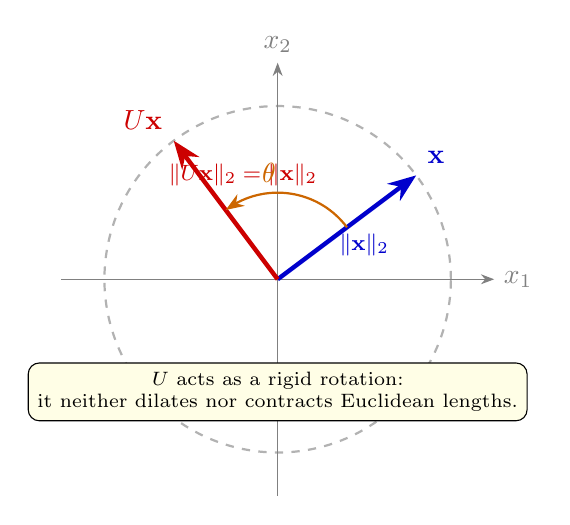
\begin{tikzpicture}[scale=1.1, >=Stealth]
    % Unit circle S_2
    \draw[dashed, gray!60, thick] (0, 0) circle (2.0);
    \draw[->, thin, gray] (-2.5, 0) -- (2.5, 0) node[right] {$x_1$};
    \draw[->, thin, gray] (0, -2.5) -- (0, 2.5) node[above] {$x_2$};

    % Original vector x
    \draw[->, ultra thick, blue!80!black] (0, 0) -- (1.6, 1.2) node[above right] {$\mathbf{x}$};
    \node[blue!80!black, font=\footnotesize] at (1.0, 0.4) {$\|\mathbf{x}\|_2$};

    % Rotated vector Ux
    \draw[->, ultra thick, red!80!black] (0, 0) -- (-1.2, 1.6) node[above left] {$U\mathbf{x}$};
    \node[red!80!black, font=\footnotesize] at (-0.4, 1.2) {$\|U\mathbf{x}\|_2 = \|\mathbf{x}\|_2$};

    % Angle arc theta
    \draw[->, thick, orange!80!black] (0.8, 0.6) arc (36.87:126.87:1.0);
    \node[orange!80!black, above] at (-0.1, 1.0) {$\theta$};

    \node[draw, rounded corners, fill=yellow!10, align=center, font=\scriptsize] at (0, -1.3) {
        $U$ acts as a rigid rotation: \\
        it neither dilates nor contracts Euclidean lengths.
    };
\end{tikzpicture}
\caption{Euclidean isometry of orthogonal transformation $U$: length conservation and rigid rotation.}
\label{fig:orthogonal-isometry}
\end{figure}

\begin{noteblock}{Fundamental Numerical Significance of Isometry}
The identity $\|U\mathbf{x}\|_2 = \|\mathbf{x}\|_2$ is the theoretical backbone of backward error stability in numerical linear algebra. Since orthogonal matrices cannot amplify vector norms, multiplying an error or perturbation $\mathbf{e}$ by $U$:
\begin{equation}
    \|U(\mathbf{x} + \mathbf{e}) - U\mathbf{x}\|_2 = \|U\mathbf{e}\|_2 = \|\mathbf{e}\|_2
\end{equation}
\textbf{preserves the exact magnitude of the perturbation} without magnification. Algorithms built on orthogonal transformations (Householder reflectors, Givens rotations, and QR factorizations) provide exceptional backward stability guarantees.
\end{noteblock}

\clearpage
\section{Chapter Summary Reference}

Table~\ref{tab:lecture-2-summary} summarizes the key analytical formulas, complexities, and properties developed in this chapter.

\begin{table}[H]
\centering
\resizebox{\textwidth}{!}{%
\begin{tabular}{l l l}
\toprule
\textbf{Property / Object} & \textbf{Mathematical Formulation} & \textbf{Key Characteristic} \\
\midrule
Matrix Multiplication & $C_{ij} = \sum_{k=1}^m A_{ik} B_{kj}$ & Requires $A \in \R^{n \times m}, B \in \R^{m \times p}$ \\
Square Product Cost & $2n^3 - n^2 \text{ FLOPs} \implies \BigO{n^3}$ & Cubic law: $T(2n) \approx 8 T(n)$ \\
Rank-Nullity Theorem & $\dim(\mathrm{Im}(A)) + \dim(\ker(A)) = m$ & $m$ is number of columns of $A$ \\
Orthonormal Vectors & $\langle \mathbf{u}_i, \mathbf{u}_j \rangle = \delta_{ij}$ & Mutually orthogonal, $\|\mathbf{u}_i\|_2 = 1$ \\
Orthogonal Matrix & $U^T U = U U^T = I_n$ & Equivalent to $U^{-1} = U^T$ \\
Rows and Columns of $U$ & Form orthonormal bases of $\R^n$ & Direct consequence of $U^T U = I_n$ \\
Entries of Orthogonal $U$ & $-1 \le U_{ij} \le 1$ & Derived from $\sum_{i=1}^n U_{ij}^2 = 1$ \\
Orthogonal Diagonal Matrix & $D = \diag(\pm 1, \dots, \pm 1)$ & $2^n$ distinct matrices in $\R^{n \times n}$ \\
Orthogonal Triangular Matrix & $R = \diag(\pm 1, \dots, \pm 1)$ & Column induction proof \\
Euclidean Isometry & $\|U\mathbf{x}\|_2 = \|\mathbf{x}\|_2$ & Rigid map: length-preserving \\
Inner Product Invariance & $\langle U\mathbf{x}, U\mathbf{y} \rangle = \langle \mathbf{x}, \mathbf{y} \rangle$ & Preserves angles between vectors \\
Transpose of Product & $(AB)^T = B^T A^T$ & Reverses factor order \\
\bottomrule
\end{tabular}%
}
\caption{Comprehensive reference table of definitions, computational complexities, and orthogonal matrix properties.}
\label{tab:lecture-2-summary}
\end{table}

\chapter[Orthonormal Matrices, Eigenvalues, and Quadratic Forms]{Matrices with Orthonormal Columns, Eigenvalues,\\Spectral Decomposition, and Quadratic Forms}
\label{chap:orthonormal-matrices-eigenvalues-quadratic-forms}

This chapter investigates the algebraic and geometric properties of rectangular matrices with orthonormal columns, systematically comparing the products $V^T V$ and $V V^T$. We then introduce spectral theory, the notions of eigenvalue and eigenvector, diagonalization, and outer product (dyadic) expansion, culminating in the Spectral Theorem for symmetric matrices. Finally, we analyze quadratic forms, the Rayleigh quotient inequality, the classification of symmetric positive definite and semidefinite matrices (SPD and SPSD), and the natural emergence of positive semidefinite structures via the Gram matrices $B^T B$ and $B B^T$~\cite{trefethen1997numerical}.

\FloatBarrier
\section{Review of Square Orthogonal Matrices and Isometry}

In the preceding chapter, we introduced the concept of an orthogonal matrix in Euclidean space $\R^n$. We briefly summarize the equivalent formulations that govern its behavior.

\begin{definition}[Equivalent Characterizations of a Square Orthogonal Matrix]
\label{def:square-orthogonal-recap}
A square matrix $U \in \R^{n \times n}$ is said to be \textbf{orthogonal} if it satisfies any of the following mutually equivalent conditions:
\begin{enumerate}
    \item $U^T U = I_n$, meaning its inverse coincides with its transpose ($U^{-1} = U^T$).
    \item $U U^T = I_n$.
    \item The set of columns of $U = [\mathbf{u}_1, \dots, \mathbf{u}_n]$ forms an orthonormal basis of $\R^n$:
    \begin{equation}
        \langle \mathbf{u}_i, \mathbf{u}_j \rangle = \mathbf{u}_i^T \mathbf{u}_j = \delta_{ij} = \begin{cases} 1 & \text{if } i = j, \\ 0 & \text{if } i \neq j. \end{cases}
    \end{equation}
    \item The set of rows of $U$ forms an orthonormal basis of $\R^n$.
\end{enumerate}
\end{definition}

\begin{noteblock}{Historical Terminological Clarification}
In mathematical literature, the term \textit{orthogonal matrix} is standard, although the columns (and rows) of such a matrix are not merely pairwise orthogonal, but also \textbf{normalized to unit length}, forming an explicitly \textbf{orthonormal} system.
\end{noteblock}

The key geometric property of an orthogonal transformation is the preservation of Euclidean distances and norms, formalized as isometry.

\begin{property}[Euclidean Isometry]
\label{prop:square-euclidean-isometry}
Let $U \in \R^{n \times n}$ be an orthogonal matrix. For every vector $\mathbf{x} \in \R^n$, the linear map preserves the Euclidean norm exactly:
\begin{equation}
    \|U\mathbf{x}\|_2 = \|\mathbf{x}\|_2.
\end{equation}
\end{property}

\begin{proof}
Evaluating the squared Euclidean norm of $U\mathbf{x}$ and applying the identity $(U\mathbf{x})^T = \mathbf{x}^T U^T$:
\begin{equation}
    \|U\mathbf{x}\|_2^2 = (U\mathbf{x})^T (U\mathbf{x}) = \mathbf{x}^T (U^T U) \mathbf{x} = \mathbf{x}^T I_n \mathbf{x} = \mathbf{x}^T \mathbf{x} = \|\mathbf{x}\|_2^2.
\end{equation}
Taking the principal square root yields $\|U\mathbf{x}\|_2 = \|\mathbf{x}\|_2$.
\end{proof}

\FloatBarrier
\section[Rectangular Matrices with Orthonormal Columns]{Rectangular Matrices with Orthonormal Columns: \texorpdfstring{$V^T V$}{V\textasciicircum T V} vs \texorpdfstring{$V V^T$}{V V\textasciicircum T}}

In computational settings (such as dimensionality reduction, principal component analysis, and thin singular value decomposition), one routinely works with rectangular matrices whose columns form an orthonormal system.

\subsection{Definition and Dimensional Constraint}

\begin{definition}[Rectangular Matrix with Orthonormal Columns]
A matrix $V \in \R^{n \times k}$ with $k < n$ (a tall-skinny matrix) has orthonormal columns if:
\begin{equation}
    V = \begin{bmatrix} \mid & \mid & & \mid \\ \mathbf{v}_1 & \mathbf{v}_2 & \dots & \mathbf{v}_k \\ \mid & \mid & & \mid \end{bmatrix}, \qquad \mathbf{v}_i \in \R^n,
\end{equation}
with column vectors satisfying the orthonormality condition:
\begin{equation}
    \langle \mathbf{v}_i, \mathbf{v}_j \rangle = \mathbf{v}_i^T \mathbf{v}_j = \delta_{ij} \quad \forall i, j \in \{1, \dots, k\}.
\end{equation}
\end{definition}

\begin{alertblock}{Dimensional Constraint: Why Must $k \le n$?}
In an $n$-dimensional vector space such as $\R^n$, any subspace has dimension at most $n$. Because any finite set of orthonormal vectors is inherently linearly independent, there cannot exist more than $n$ orthonormal vectors in $\R^n$. Consequently, a matrix with orthonormal columns can possess at most as many columns as it has rows ($k \le n$).
\end{alertblock}

\subsection{The Inner Product \texorpdfstring{$V^T V$}{V\textasciicircum T V} (Column Gramian)}

Consider the product of the transpose $V^T \in \R^{k \times n}$ and $V \in \R^{n \times k}$. The result is a square matrix of order $k$:
\begin{equation}
    V^T V \in \R^{k \times k}.
\end{equation}
Expanding the block multiplication, representing $V^T$ by rows and $V$ by columns:
\begin{equation}
    V^T V = \begin{bmatrix} \text{---} & \mathbf{v}_1^T & \text{---} \\ \text{---} & \mathbf{v}_2^T & \text{---} \\ & \vdots & \\ \text{---} & \mathbf{v}_k^T & \text{---} \end{bmatrix} \begin{bmatrix} \mid & \mid & & \mid \\ \mathbf{v}_1 & \mathbf{v}_2 & \dots & \mathbf{v}_k \\ \mid & \mid & & \mid \end{bmatrix} = \begin{bmatrix} \mathbf{v}_1^T \mathbf{v}_1 & \mathbf{v}_1^T \mathbf{v}_2 & \dots & \mathbf{v}_1^T \mathbf{v}_k \\ \mathbf{v}_2^T \mathbf{v}_1 & \mathbf{v}_2^T \mathbf{v}_2 & \dots & \mathbf{v}_2^T \mathbf{v}_k \\ \vdots & \vdots & \ddots & \vdots \\ \mathbf{v}_k^T \mathbf{v}_1 & \mathbf{v}_k^T \mathbf{v}_2 & \dots & \mathbf{v}_k^T \mathbf{v}_k \end{bmatrix}.
\end{equation}
Applying orthonormality $\mathbf{v}_i^T \mathbf{v}_j = \delta_{ij}$, this matrix evaluates precisely to the $k \times k$ identity matrix:
\begin{equation}
    V^T V = I_k.
\end{equation}

\subsection{The Reversed Product \texorpdfstring{$V V^T$}{V V\textasciicircum T} (Orthogonal Projector)}

Reversing the order of multiplication yields a square matrix of substantially larger size, $n \times n$:
\begin{equation}
    V V^T \in \R^{n \times n}.
\end{equation}

\begin{theorem}[Non-Identity of $V V^T$]
Let $V \in \R^{n \times k}$ have orthonormal columns with $k < n$. Then:
\begin{equation}
    V V^T \neq I_n.
\end{equation}
\end{theorem}

\begin{proof}
The proof relies on the rank inequality for matrix products:
\begin{enumerate}
    \item The rank of a matrix product is bounded by the rank of its factors:
    \begin{equation}
        \rank(V V^T) \le \min\big(\rank(V), \, \rank(V^T)\big).
    \end{equation}
    \item Since the $k$ columns of $V$ are orthonormal and hence linearly independent, $\rank(V) = \rank(V^T) = k$.
    \item Therefore, $\rank(V V^T) \le k$. In fact, because $V^T V = I_k$, we have exactly $\rank(V V^T) = k$.
    \item On the other hand, the identity matrix $I_n \in \R^{n \times n}$ has full rank $n$.
    \item Because $k < n$ by assumption:
    \begin{equation}
        \rank(V V^T) = k < n = \rank(I_n) \implies V V^T \neq I_n.
    \end{equation}
\end{enumerate}
The matrix $V V^T$ is singular and possesses a non-trivial null space of dimension $n - k > 0$.
\end{proof}

\subsubsection{Outer Product Expansion and Geometric Interpretation}
By block partition, the product $V V^T$ can be expressed as a sum of outer products (dyads):
\begin{equation}
    V V^T = \sum_{i=1}^k \mathbf{v}_i \mathbf{v}_i^T = \mathbf{v}_1 \mathbf{v}_1^T + \mathbf{v}_2 \mathbf{v}_2^T + \dots + \mathbf{v}_k \mathbf{v}_k^T.
\end{equation}
Each term $\mathbf{v}_i \mathbf{v}_i^T$ is a symmetric rank-1 matrix of size $n \times n$. The operator $P = V V^T$:
\begin{itemize}
    \item Is idempotent: $P^2 = (V V^T)(V V^T) = V (V^T V) V^T = V I_k V^T = V V^T = P$.
    \item Is symmetric: $P^T = (V V^T)^T = (V^T)^T V^T = V V^T = P$.
\end{itemize}
Hence, $P = V V^T$ is the \textbf{orthogonal projector} from $\R^n$ onto the $k$-dimensional subspace:
\begin{equation}
    \mathcal{S} = \spanop\{\mathbf{v}_1, \dots, \mathbf{v}_k\}.
\end{equation}

\begin{figure}[H]
\centering
\resizebox{0.95\textwidth}{!}{%
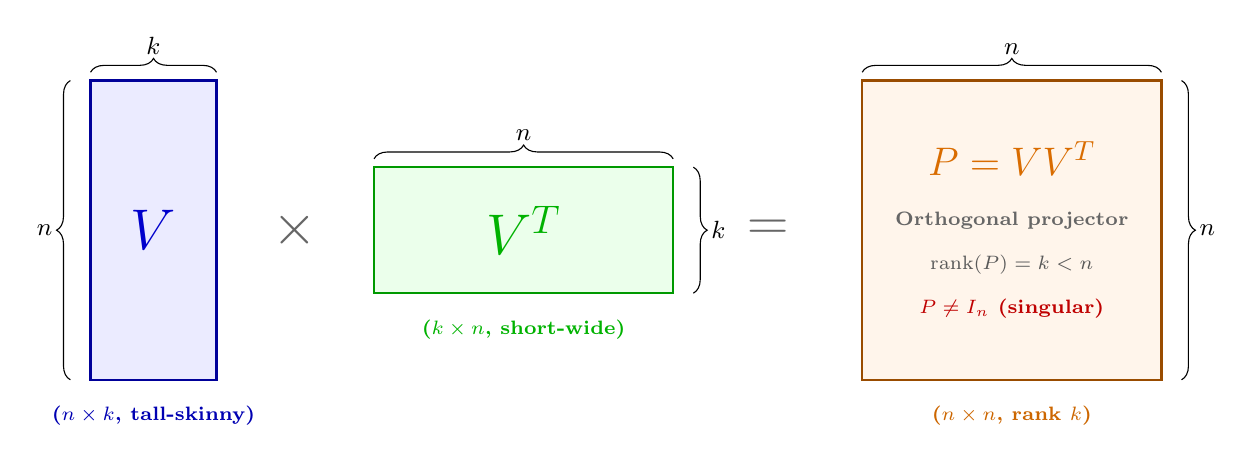
\begin{tikzpicture}[>=Stealth,
    brace/.style={decorate, decoration={brace, amplitude=5pt, raise=3pt}}]
    % --- Matrix V (n x k, tall-skinny) ---
    \draw[thick, fill=blue!8, draw=blue!60!black] (0, 0) rectangle (1.6, 3.8);
    \node[font=\bfseries\huge, text=blue!80!black] at (0.8, 1.9) {$V$};
    \node[below=6pt, font=\scriptsize\bfseries, text=blue!70!black] at (0.8, 0) {($n \times k$, tall-skinny)};
    % Dimension braces of V (facing outward)
    \draw[brace] (-0.15, 0) -- (-0.15, 3.8) node[midway, left=6pt, font=\small] {$n$};
    \draw[brace] (0, 3.8) -- (1.6, 3.8) node[midway, above=6pt, font=\small] {$k$};

    % Multiplication operator
    \node[font=\huge, text=gray!80!black] at (2.6, 1.9) {$\times$};

    % --- Matrix V^T (k x n, short-wide) ---
    \draw[thick, fill=green!8, draw=green!60!black] (3.6, 1.1) rectangle (7.4, 2.7);
    \node[font=\bfseries\huge, text=green!70!black] at (5.5, 1.9) {$V^T$};
    \node[below=6pt, font=\scriptsize\bfseries, text=green!70!black] at (5.5, 1.1) {($k \times n$, short-wide)};
    % Dimension braces of V^T (facing outward)
    \draw[brace] (3.6, 2.7) -- (7.4, 2.7) node[midway, above=6pt, font=\small] {$n$};
    \draw[brace] (7.55, 2.7) -- (7.55, 1.1) node[midway, right=6pt, font=\small] {$k$};

    % Equals operator
    \node[font=\huge, text=gray!80!black] at (8.6, 1.9) {$=$};

    % --- Resulting Matrix V V^T = P (n x n) ---
    \draw[thick, fill=orange!8, draw=orange!60!black] (9.8, 0) rectangle (13.6, 3.8);
    \node[align=center] at (11.7, 1.9) {%
        {\bfseries\Large\color{orange!85!black} $P = V V^T$}\\[6pt]
        {\scriptsize\bfseries\color{gray!80!black} Orthogonal projector}\\[4pt]
        {\scriptsize\color{gray!70!black} $\rank(P) = k < n$}\\[4pt]
        {\scriptsize\bfseries\color{red!75!black} $P \neq I_n$ (singular)}%
    };
    \node[below=6pt, font=\scriptsize\bfseries, text=orange!80!black] at (11.7, 0) {($n \times n$, rank $k$)};
    % Dimension braces of V V^T (facing outward)
    \draw[brace] (9.8, 3.8) -- (13.6, 3.8) node[midway, above=6pt, font=\small] {$n$};
    \draw[brace] (13.75, 3.8) -- (13.75, 0) node[midway, right=6pt, font=\small] {$n$};
\end{tikzpicture}%
}
\caption{Dimension and rank comparison: the product $V V^T$ yields an $n \times n$ orthogonal projector with strictly deficient rank $k < n$.}
\label{fig:v-vt-projector}
\end{figure}

\FloatBarrier
\section[Partial Isometry for Orthonormal Matrices]{Partial Isometry for Rectangular\\Orthonormal Matrices}

In the rectangular setting ($V \in \R^{n \times k}$ with $k < n$), the isometric property applies asymmetrically depending on the domain of the input vector.

\subsection{Question (a): Norm Preservation for Vectors in \texorpdfstring{$\R^k$}{R\textasciicircum k}}

\begin{proposition}[Right Isometry]
\label{prop:right-isometry}
Let $V \in \R^{n \times k}$ have orthonormal columns with $k < n$. For any vector $\mathbf{x} \in \R^k$:
\begin{equation}
    \|V\mathbf{x}\|_2 = \|\mathbf{x}\|_2.
\end{equation}
\end{proposition}

\begin{proof}
Compute the squared Euclidean norm of $V\mathbf{x} \in \R^n$:
\begin{equation}
    \|V\mathbf{x}\|_2^2 = (V\mathbf{x})^T (V\mathbf{x}) = \mathbf{x}^T (V^T V) \mathbf{x}.
\end{equation}
Since the columns of $V$ are orthonormal, $V^T V = I_k$. Substituting:
\begin{equation}
    \|V\mathbf{x}\|_2^2 = \mathbf{x}^T I_k \mathbf{x} = \mathbf{x}^T \mathbf{x} = \|\mathbf{x}\|_2^2.
\end{equation}
Taking the positive square root yields $\|V\mathbf{x}\|_2 = \|\mathbf{x}\|_2$ for all $\mathbf{x} \in \R^k$.
\end{proof}

\begin{noteblock}{Geometric Interpretation}
The mapping $V: \R^k \to \R^n$ is an \textbf{isometric embedding}: it embeds the lower-dimensional space $\R^k$ into a $k$-dimensional subspace of $\R^n$ while strictly preserving all vector lengths and angles.
\end{noteblock}

\subsection{Question (b): Norm Preservation for Vectors in \texorpdfstring{$\R^n$}{R\textasciicircum n} under \texorpdfstring{$V^T$}{V\textasciicircum T}}

\begin{proposition}[Failure of Left Isometry]
\label{prop:left-non-isometry}
Let $V \in \R^{n \times k}$ have orthonormal columns with $k < n$. The transposed operator $V^T: \R^n \to \R^k$ does \textbf{not} preserve the Euclidean norm across all of $\R^n$:
\begin{equation}
    \exists \mathbf{y} \in \R^n \quad \text{such that} \quad \|V^T \mathbf{y}\|_2 \neq \|\mathbf{y}\|_2.
\end{equation}
\end{proposition}

\begin{proof}
Evaluate the squared Euclidean norm of $V^T \mathbf{y}$:
\begin{equation}
    \|V^T \mathbf{y}\|_2^2 = (V^T \mathbf{y})^T (V^T \mathbf{y}) = \mathbf{y}^T (V V^T) \mathbf{y}.
\end{equation}
Because $V V^T \neq I_n$, this expression does not collapse identically to $\|\mathbf{y}\|_2^2$.

\medskip
\noindent\textbf{Null-Space Counterexample:}
Consider the matrix $V^T \in \R^{k \times n}$. By the Rank-Nullity Theorem:
\begin{equation}
    \dim(\ker(V^T)) = n - \rank(V^T) = n - k.
\end{equation}
Since $k < n$, the null-space dimension is strictly positive ($n - k > 0$). There exists a non-zero vector $\tilde{\mathbf{y}} \in \R^n \setminus \{\mathbf{0}\}$ such that:
\begin{equation}
    \tilde{\mathbf{y}} \in \ker(V^T) \implies V^T \tilde{\mathbf{y}} = \mathbf{0} \in \R^k.
\end{equation}
Computing norms:
\begin{equation}
    \|V^T \tilde{\mathbf{y}}\|_2 = \|\mathbf{0}\|_2 = 0 \neq \|\tilde{\mathbf{y}}\|_2.
\end{equation}
Thus, norm shrinkage is maximal for any vector orthogonal to the subspace spanned by the columns of $V$.
\end{proof}

\FloatBarrier
\section{Eigenvalues and Eigenvectors: Foundations and Step-by-Step Example}

\subsection{Fundamental Definitions}

Let $A \in \R^{n \times n}$ be a \textbf{square} matrix.

\begin{definition}[Eigenvalue, Eigenvector, and Eigenpair]
\label{def:eigenvalue-eigenvector}
A scalar $\lambda \in \R$ (or in $\C$) is called an \textbf{eigenvalue} of $A$ if there exists a \textbf{non-zero} vector $\mathbf{v} \in \R^n \setminus \{\mathbf{0}\}$ (or $\C^n \setminus \{\mathbf{0}\}$) such that:
\begin{equation}
    A\mathbf{v} = \lambda \mathbf{v}.
\end{equation}
The vector $\mathbf{v}$ is termed an \textbf{eigenvector} associated with $\lambda$. The pair $(\lambda, \mathbf{v})$ is called an \textbf{eigenpair}.
\end{definition}

The eigenvalue equation $A\mathbf{v} = \lambda \mathbf{v}$ can be recast as a homogeneous linear system:
\begin{equation}
    (A - \lambda I_n)\mathbf{v} = \mathbf{0}.
\end{equation}
For non-trivial solutions ($\mathbf{v} \neq \mathbf{0}$) to exist, the coefficient matrix $(A - \lambda I_n)$ must be singular, meaning its determinant vanishes:
\begin{equation}
    p(\lambda) = \det(A - \lambda I_n) = 0.
\end{equation}
The polynomial $p(\lambda)$ is the \textbf{characteristic polynomial} of $A$, of degree $n$. The eigenvalues of $A$ are precisely the roots of this characteristic polynomial.

\subsection{Step-by-Step Worked Example}

\begin{example}[Computing Eigenvalues and Eigenvectors for a $2 \times 2$ Matrix]
\label{ex:eigenvalues-2x2}
Consider the real symmetric matrix:
\begin{equation}
    A = \begin{bmatrix} 2 & 1 \\ 1 & 2 \end{bmatrix} \in \R^{2 \times 2}.
\end{equation}

\noindent\textbf{Step 1: Characteristic Polynomial and Eigenvalues.}
\begin{equation}
    p(\lambda) = \det(A - \lambda I_2) = \det \begin{bmatrix} 2-\lambda & 1 \\ 1 & 2-\lambda \end{bmatrix} = (2-\lambda)^2 - 1.
\end{equation}
Using the difference of squares factorization $a^2 - b^2 = (a-b)(a+b)$:
\begin{equation}
    p(\lambda) = \big((2-\lambda) - 1\big)\big((2-\lambda) + 1\big) = (1-\lambda)(3-\lambda) = 0.
\end{equation}
Setting $p(\lambda) = 0$ yields the eigenvalues:
\begin{equation}
    \lambda_1 = 3, \quad \lambda_2 = 1.
\end{equation}

\noindent\textbf{Step 2: Eigenvector for $\lambda_1 = 3$.}
We solve $(A - 3I_2)\mathbf{v}_1 = \mathbf{0}$:
\begin{equation}
    \begin{bmatrix} 2-3 & 1 \\ 1 & 2-3 \end{bmatrix} \begin{bmatrix} x \\ y \end{bmatrix} = \begin{bmatrix} -1 & 1 \\ 1 & -1 \end{bmatrix} \begin{bmatrix} x \\ y \end{bmatrix} = \begin{bmatrix} 0 \\ 0 \end{bmatrix} \implies -x + y = 0 \iff y = x.
\end{equation}
Choosing $x = 1$, we obtain the eigenvector:
\begin{equation}
    \mathbf{v}_1 = \begin{bmatrix} 1 \\ 1 \end{bmatrix}.
\end{equation}

\noindent\textbf{Step 3: Eigenvector for $\lambda_2 = 1$.}
We solve $(A - I_2)\mathbf{v}_2 = \mathbf{0}$:
\begin{equation}
    \begin{bmatrix} 2-1 & 1 \\ 1 & 2-1 \end{bmatrix} \begin{bmatrix} x \\ y \end{bmatrix} = \begin{bmatrix} 1 & 1 \\ 1 & 1 \end{bmatrix} \begin{bmatrix} x \\ y \end{bmatrix} = \begin{bmatrix} 0 \\ 0 \end{bmatrix} \implies x + y = 0 \iff y = -x.
\end{equation}
Choosing $x = 1$, we find the eigenvector:
\begin{equation}
    \mathbf{v}_2 = \begin{bmatrix} 1 \\ -1 \end{bmatrix}.
\end{equation}
Notice that $\mathbf{v}_1^T \mathbf{v}_2 = 1(1) + 1(-1) = 0$: the two eigenvectors are mutually orthogonal.
\end{example}

\FloatBarrier
\section{Diagonalization and Dyadic Expansion}

\subsection{Diagonalizable Matrices}

\begin{definition}[Diagonalizability]
A matrix $A \in \R^{n \times n}$ is called \textbf{diagonalizable} if it possesses $n$ linearly independent eigenvectors, that is, if there exists a basis of $\R^n$ consisting of eigenvectors of $A$.
\end{definition}

In this case, assembling the $n$ eigenvectors into the modal matrix $V = [\mathbf{v}_1, \dots, \mathbf{v}_n] \in \R^{n \times n}$ and the eigenvalues along the diagonal matrix $D = \diag(\lambda_1, \dots, \lambda_n)$:
\begin{equation}
    A V = A [\mathbf{v}_1, \dots, \mathbf{v}_n] = [\lambda_1 \mathbf{v}_1, \dots, \lambda_n \mathbf{v}_n] = [\mathbf{v}_1, \dots, \mathbf{v}_n] \begin{bmatrix} \lambda_1 & & \\ & \ddots & \\ & & \lambda_n \end{bmatrix} = V D.
\end{equation}
Because the eigenvectors are linearly independent, $V$ is invertible. Multiplying on the right by $V^{-1}$:
\begin{equation}
    A = V D V^{-1}.
\end{equation}

\subsection{Dyadic (Outer Product) Expansion}

Let $W = V^{-1} \in \R^{n \times n}$, partitioned by rows:
\begin{equation}
    W = V^{-1} = \begin{bmatrix} \text{---} & \mathbf{w}_1^T & \text{---} \\ \text{---} & \mathbf{w}_2^T & \text{---} \\ & \vdots & \\ \text{---} & \mathbf{w}_n^T & \text{---} \end{bmatrix}.
\end{equation}
Because $W V = I_n$, the rows of $W$ and columns of $V$ satisfy biorthonormality: $\mathbf{w}_i^T \mathbf{v}_j = \delta_{ij}$. Expanding $A = V D W$:
\begin{align}
    A &= \begin{bmatrix} \mid & & \mid \\ \mathbf{v}_1 & \dots & \mathbf{v}_n \\ \mid & & \mid \end{bmatrix} \begin{bmatrix} \lambda_1 & & \\ & \ddots & \\ & & \lambda_n \end{bmatrix} \begin{bmatrix} \text{---} & \mathbf{w}_1^T & \text{---} \\ & \vdots & \\ \text{---} & \mathbf{w}_n^T & \text{---} \end{bmatrix} \nonumber \\
    &= \begin{bmatrix} \mid & & \mid \\ \lambda_1 \mathbf{v}_1 & \dots & \lambda_n \mathbf{v}_n \\ \mid & & \mid \end{bmatrix} \begin{bmatrix} \text{---} & \mathbf{w}_1^T & \text{---} \\ & \vdots & \\ \text{---} & \mathbf{w}_n^T & \text{---} \end{bmatrix}.
\end{align}
Performing block column-by-row multiplication yields the dyadic expansion:
\begin{equation}
    A = \sum_{i=1}^n \lambda_i \mathbf{v}_i \mathbf{w}_i^T = \lambda_1 \mathbf{v}_1 \mathbf{w}_1^T + \lambda_2 \mathbf{v}_2 \mathbf{w}_2^T + \dots + \lambda_n \mathbf{v}_n \mathbf{w}_n^T.
\end{equation}

\begin{noteblock}{Significance of the Dyadic Expansion}
The matrix $A$ is represented as a weighted sum of $n$ elementary rank-1 matrices, each formed by the outer product $\mathbf{v}_i \mathbf{w}_i^T$. The eigenvalues $\lambda_i$ serve as modulation weights. This structure serves as the direct precursor to the Singular Value Decomposition (SVD) and the Eckart-Young-Mirsky low-rank approximation theorem.
\end{noteblock}

\subsection{Pathologies: When Diagonalization Fails}

Not all matrices admit a decomposition $A = V D V^{-1}$ over the real numbers. Two distinct theoretical obstacles exist.

\subsubsection{Case 1: Absence of Real Eigenvalues}
Consider the $90^\circ$ planar rotation matrix:
\begin{equation}
    A = \begin{bmatrix} 0 & -1 \\ 1 & 0 \end{bmatrix}.
\end{equation}
Its characteristic polynomial is:
\begin{equation}
    p(\lambda) = \det \begin{bmatrix} -\lambda & -1 \\ 1 & -\lambda \end{bmatrix} = \lambda^2 + 1 = 0 \implies \lambda_{1,2} = \pm i \notin \R.
\end{equation}
Although $A$ has purely real entries, it \textbf{admits no real eigenvalues or real eigenvectors}. Geometrically, a non-trivial planar rotation does not preserve the direction of any real vector in $\R^2$.

\subsubsection{Case 2: Defective Matrices (Geometric Multiplicity Strictly Less than Algebraic)}
Consider the shear matrix:
\begin{equation}
    A = \begin{bmatrix} 1 & 1 \\ 0 & 1 \end{bmatrix}.
\end{equation}
\begin{enumerate}
    \item The characteristic polynomial is $p(\lambda) = (1-\lambda)^2 = 0$. There is a single eigenvalue $\lambda = 1$ with \textbf{algebraic multiplicity} $m_a(1) = 2$.
    \item We determine its \textbf{geometric multiplicity} $m_g(1) = \dim(\ker(A - I_2))$:
    \begin{equation}
        A - I_2 = \begin{bmatrix} 0 & 1 \\ 0 & 0 \end{bmatrix} \implies \begin{bmatrix} 0 & 1 \\ 0 & 0 \end{bmatrix} \begin{bmatrix} x \\ y \end{bmatrix} = \begin{bmatrix} 0 \\ 0 \end{bmatrix} \implies y = 0, \quad x \in \R \text{ free}.
    \end{equation}
    The eigenspace is one-dimensional: $\ker(A - I_2) = \spanop\left\{\begin{bmatrix} 1 \\ 0 \end{bmatrix}\right\}$, so $m_g(1) = 1$.
\end{enumerate}
Since $m_g(1) = 1 < 2 = m_a(1)$, it is impossible to find 2 linearly independent eigenvectors to form $V$. The matrix $A$ is termed \textbf{defective} and cannot be diagonalized (it admits only a Jordan canonical form).

\FloatBarrier
\section{Guided Exercises on Eigenvalues (Q1 -- Q4)}

\subsection{Exercise Q1: Eigenpairs of a Diagonal Matrix}

\begin{example}[Spectrum of a Diagonal Matrix]
\label{ex:q1-diagonal-matrix}
Given a generic diagonal matrix $D = \diag(d_1, d_2, \dots, d_n) \in \R^{n \times n}$, we determine its eigenpairs.

\noindent\textbf{Solution:}
Examine the action of $D$ on the $i$-th standard basis vector $\mathbf{e}_i = [0, \dots, 1, \dots, 0]^T$:
\begin{equation}
    D \mathbf{e}_i = \begin{bmatrix} d_1 & & & \\ & d_2 & & \\ & & \ddots & \\ & & & d_n \end{bmatrix} \begin{bmatrix} 0 \\ \vdots \\ 1 \\ \vdots \\ 0 \end{bmatrix} = \begin{bmatrix} 0 \\ \vdots \\ d_i \\ \vdots \\ 0 \end{bmatrix} = d_i \mathbf{e}_i.
\end{equation}
Therefore:
\begin{itemize}
    \item The eigenvalues are precisely the entries along the main diagonal: $\lambda_i = d_i$ for $i = 1, \dots, n$.
    \item The corresponding eigenvectors are the standard basis vectors: $\mathbf{v}_i = \mathbf{e}_i$.
    \item The canonical eigenpairs are $(d_1, \mathbf{e}_1), (d_2, \mathbf{e}_2), \dots, (d_n, \mathbf{e}_n)$.
\end{itemize}
\end{example}

\begin{property}[Coinciding Eigenvalues and Eigenspace Structure]
What happens if two or more diagonal entries coincide, for example $d_1 = d_2 = \lambda$?
In this case, \textbf{any linear combination} $\alpha \mathbf{e}_1 + \beta \mathbf{e}_2$ (with $\alpha, \beta$ not both zero) remains an eigenvector corresponding to $\lambda$.

\medskip
\noindent\textit{General proof:} Let $\mathbf{v}, \mathbf{w} \in \R^n$ be two eigenvectors of an arbitrary matrix $A$ associated with the \textbf{same} eigenvalue $\lambda$ ($A\mathbf{v} = \lambda \mathbf{v}$ and $A\mathbf{w} = \lambda \mathbf{w}$). For any scalars $\alpha, \beta \in \R$:
\begin{equation}
    A(\alpha \mathbf{v} + \beta \mathbf{w}) = \alpha (A\mathbf{v}) + \beta (A\mathbf{w}) = \alpha (\lambda \mathbf{v}) + \beta (\lambda \mathbf{w}) = \lambda (\alpha \mathbf{v} + \beta \mathbf{w}).
\end{equation}
Hence, the set of eigenvectors associated with $\lambda$, together with the zero vector, forms a closed vector subspace known as the \textbf{eigenspace}:
\begin{equation}
    \mathcal{E}(\lambda) = \ker(A - \lambda I_n).
\end{equation}
\end{property}

\subsection{Exercise Q2: Eigenpairs of the Identity Matrix}

\begin{example}[Spectrum of the Identity Matrix]
\label{ex:q2-identity-matrix}
Determine the eigenvalues and eigenvectors of the identity matrix $I_n \in \R^{n \times n}$.

\noindent\textbf{Solution:}
By definition of the identity operator, for every non-zero vector $\mathbf{x} \in \R^n \setminus \{\mathbf{0}\}$:
\begin{equation}
    I_n \mathbf{x} = 1 \cdot \mathbf{x}.
\end{equation}
\begin{itemize}
    \item \textbf{Eigenvalue:} $\lambda = 1$ with algebraic and geometric multiplicity $n$ ($m_a = m_g = n$).
    \item \textbf{Eigenvectors:} \textbf{every} non-zero vector in $\R^n$.
    \item The entire space $\R^n$ constitutes the eigenspace: $\mathcal{E}(1) = \R^n$.
\end{itemize}
\end{example}

\subsection{Exercise Q3: Sum and Product of Matrices Sharing an Eigenvalue}

\begin{example}[Eigenvalues of Matrix Sum and Product]
\label{ex:q3-sum-product}
Let $\lambda \in \R$ be a common eigenvalue of $A \in \R^{n \times n}$ and $B \in \R^{n \times n}$.
\begin{enumerate}
    \item Is $2\lambda$ necessarily an eigenvalue of $A + B$?
    \item Is $\lambda^2$ necessarily an eigenvalue of $AB$?
\end{enumerate}

\noindent\textbf{Analytical Answer: NO to both questions.}
For eigenvalue addition or multiplication to hold, $A$ and $B$ must share the \textbf{same eigenvector} associated with $\lambda$. If their eigenvectors are misaligned, the property fails.

\medskip
\noindent\textbf{Counterexample for Summation:}
Consider:
\begin{equation}
    A = \begin{bmatrix} 5 & 0 \\ 0 & 1 \end{bmatrix}, \quad B = \begin{bmatrix} 1 & 0 \\ 0 & 5 \end{bmatrix}.
\end{equation}
Both matrices possess the eigenvalue set $\{1, 5\}$ (in particular, sharing $\lambda = 1$ and $\lambda = 5$). Compute the sum:
\begin{equation}
    A + B = \begin{bmatrix} 6 & 0 \\ 0 & 6 \end{bmatrix} = 6 I_2.
\end{equation}
The eigenvalues of $A + B$ are both equal to $6$. However, doubling the original eigenvalues gives:
\begin{equation}
    2 \cdot 1 = 2 \neq 6, \qquad 2 \cdot 5 = 10 \neq 6.
\end{equation}
Thus, $2\lambda$ does not belong to the spectrum of the sum matrix.

\medskip
\noindent\textbf{Counterexample for Multiplication:}
Consider:
\begin{equation}
    A = \begin{bmatrix} 2 & 0 \\ 0 & 3 \end{bmatrix}, \quad B = \begin{bmatrix} 10 & 0 \\ 0 & 2 \end{bmatrix}.
\end{equation}
Both matrices share the eigenvalue $\lambda = 2$. Their product evaluates to:
\begin{equation}
    AB = \begin{bmatrix} 20 & 0 \\ 0 & 6 \end{bmatrix}.
\end{equation}
The eigenvalues of $AB$ are $\{20, 6\}$, neither of which matches $\lambda^2 = 2^2 = 4$.
\end{example}

\subsection{Exercise Q4: Eigenpairs of a Matrix Power}

\begin{theorem}[Spectrum of Matrix Power $A^k$]
\label{thm:matrix-power}
Let $A \in \R^{n \times n}$ and let $(\lambda, \mathbf{v})$ be an eigenpair of $A$ ($A\mathbf{v} = \lambda \mathbf{v}$). Then for every positive integer exponent $k \in \N$:
\begin{equation}
    (\lambda^k, \mathbf{v}) \quad \text{is an eigenpair of } A^k, \quad \text{that is, } A^k \mathbf{v} = \lambda^k \mathbf{v}.
\end{equation}
\end{theorem}

\begin{proof}
The proof proceeds by induction on $k$:
\begin{enumerate}
    \item \textbf{Base Case ($k=1$):} $A^1 \mathbf{v} = A\mathbf{v} = \lambda \mathbf{v} = \lambda^1 \mathbf{v}$.
    \item \textbf{Inductive Step:} Assume $A^k \mathbf{v} = \lambda^k \mathbf{v}$. Multiplying on the left by $A$:
    \begin{equation}
        A^{k+1} \mathbf{v} = A(A^k \mathbf{v}) = A(\lambda^k \mathbf{v}) = \lambda^k (A\mathbf{v}) = \lambda^k (\lambda \mathbf{v}) = \lambda^{k+1} \mathbf{v}.
    \end{equation}
\end{enumerate}
The statement holds for all $k \ge 1$.
\end{proof}

\begin{corollary}[Power Factorization for Diagonalizable Matrices]
If $A = V D V^{-1}$ is diagonalizable, evaluating powers telescopically yields:
\begin{align}
    A^k &= (V D V^{-1})(V D V^{-1}) \cdots (V D V^{-1}) \nonumber \\
    &= V D (V^{-1}V) D \cdots (V^{-1}V) D V^{-1} = V D^k V^{-1}.
\end{align}
Since $D = \diag(\lambda_1, \dots, \lambda_n)$ is diagonal, its $k$-th power is simply:
\begin{equation}
    D^k = \diag(\lambda_1^k, \lambda_2^k, \dots, \lambda_n^k).
\end{equation}
\end{corollary}

\begin{alertblock}{Warning on Eigenvector Invariance}
Take careful note that when raising a matrix to a power, \textbf{only the eigenvalues} are raised to the power $k$, while the \textbf{eigenvectors remain strictly unchanged}. The notation $\mathbf{v}^k$ has no meaning in vector algebra.
\end{alertblock}

\FloatBarrier
\section{Symmetric Matrices and the Spectral Theorem}

Symmetric matrices represent the most important class of matrices in numerical linear algebra, optimization, and machine learning.

\begin{definition}[Symmetric Matrix]
A square matrix $A \in \R^{n \times n}$ is said to be \textbf{symmetric} if it coincides with its transpose:
\begin{equation}
    A^T = A \iff A_{ij} = A_{ji} \quad \forall i, j \in \{1, \dots, n\}.
\end{equation}
\end{definition}

\begin{theorem}[Spectral Theorem for Real Symmetric Matrices]
\label{thm:spectral-theorem}
Let $A \in \R^{n \times n}$ be a real symmetric matrix ($A^T = A$). Then:
\begin{enumerate}
    \item All $n$ eigenvalues of $A$ are \textbf{real numbers}: $\lambda_1, \lambda_2, \dots, \lambda_n \in \R$.
    \item Eigenvectors corresponding to distinct eigenvalues are mutually \textbf{orthogonal}.
    \item The matrix $A$ is \textbf{orthogonally diagonalizable}: there exist an orthogonal matrix $U \in \R^{n \times n}$ ($U^T U = U U^T = I_n$) and a real diagonal matrix $D \in \R^{n \times n}$ such that:
    \begin{equation}
        A = U D U^T.
    \end{equation}
\end{enumerate}
Equivalently, there exists an \textbf{orthonormal basis of $\R^n$ consisting entirely of eigenvectors of $A$}.
\end{theorem}

\begin{proof}[Distinct Eigenvalues]
Let $(\lambda_1, \mathbf{u}_1)$ and $(\lambda_2, \mathbf{u}_2)$ be two eigenpairs of $A$ with $\lambda_1 \neq \lambda_2$. Consider the scalar quantity $\mathbf{u}_1^T A \mathbf{u}_2$:
\begin{enumerate}
    \item Acting with $A$ to the right:
    \begin{equation}
        \mathbf{u}_1^T (A \mathbf{u}_2) = \mathbf{u}_1^T (\lambda_2 \mathbf{u}_2) = \lambda_2 (\mathbf{u}_1^T \mathbf{u}_2).
    \end{equation}
    \item Using symmetry $A = A^T$ and acting to the left:
    \begin{equation}
        \mathbf{u}_1^T A \mathbf{u}_2 = (A^T \mathbf{u}_1)^T \mathbf{u}_2 = (A \mathbf{u}_1)^T \mathbf{u}_2 = (\lambda_1 \mathbf{u}_1)^T \mathbf{u}_2 = \lambda_1 (\mathbf{u}_1^T \mathbf{u}_2).
    \end{equation}
\end{enumerate}
Equating the two expressions:
\begin{equation}
    \lambda_1 (\mathbf{u}_1^T \mathbf{u}_2) = \lambda_2 (\mathbf{u}_1^T \mathbf{u}_2) \iff (\lambda_1 - \lambda_2) (\mathbf{u}_1^T \mathbf{u}_2) = 0.
\end{equation}
Since $\lambda_1 \neq \lambda_2$ by assumption, it necessarily follows that:
\begin{equation}
    \mathbf{u}_1^T \mathbf{u}_2 = 0,
\end{equation}
proving that the eigenvectors are orthogonal.
\end{proof}

\FloatBarrier
\section{Quadratic Forms and the Rayleigh Quotient Inequality}
\label{sec:en:quadratic-forms-rayleigh}

\subsection{Definition of a Quadratic Form}

\begin{definition}[Quadratic Form]
Let $A \in \R^{n \times n}$ be a real symmetric matrix. The function $q: \R^n \to \R$ defined by:
\begin{equation}
    q(\mathbf{x}) = \mathbf{x}^T A \mathbf{x} = \sum_{i=1}^n \sum_{j=1}^n A_{ij} x_i x_j
\end{equation}
is called the \textbf{quadratic form} associated with matrix $A$.
\end{definition}

\subsection{Spectral Bounds Theorem (Rayleigh Inequality)}

\begin{theorem}[Spectral Bounds on Quadratic Forms]
\label{thm:spectral-bounds}
Let $A \in \R^{n \times n}$ be real symmetric, with eigenvalues arranged in descending order:
\begin{equation}
    \lambda_{\max} = \lambda_1 \ge \lambda_2 \ge \dots \ge \lambda_n = \lambda_{\min}.
\end{equation}
Then for every vector $\mathbf{x} \in \R^n$, the double inequality holds:
\begin{equation}
    \lambda_{\min} \|\mathbf{x}\|_2^2 \le \mathbf{x}^T A \mathbf{x} \le \lambda_{\max} \|\mathbf{x}\|_2^2.
\end{equation}
\end{theorem}

\begin{proof}
The proof proceeds systematically:
\begin{enumerate}
    \item \textbf{Spectral Factorization:} By the Spectral Theorem~\ref{thm:spectral-theorem}, we factorize $A = U D U^T$, where $U \in \R^{n \times n}$ is orthogonal and $D = \diag(\lambda_1, \dots, \lambda_n)$.
    \item \textbf{Substitution into the Quadratic Form:}
    \begin{equation}
        \mathbf{x}^T A \mathbf{x} = \mathbf{x}^T (U D U^T) \mathbf{x} = (U^T \mathbf{x})^T D (U^T \mathbf{x}).
    \end{equation}
    \item \textbf{Orthogonal Change of Coordinates:} Define $\mathbf{y} \in \R^n$ via:
    \begin{equation}
        \mathbf{y} = U^T \mathbf{x} \iff \mathbf{x} = U \mathbf{y}.
    \end{equation}
    Because $U$ is orthogonal, the map preserves Euclidean norm (Property~\ref{prop:square-euclidean-isometry}):
    \begin{equation}
        \|\mathbf{y}\|_2^2 = \|U^T \mathbf{x}\|_2^2 = \|\mathbf{x}\|_2^2 \implies \sum_{i=1}^n y_i^2 = \|\mathbf{x}\|_2^2.
    \end{equation}
    \item \textbf{Component Expansion:}
    \begin{equation}
        \mathbf{x}^T A \mathbf{x} = \mathbf{y}^T D \mathbf{y} = \sum_{i=1}^n \lambda_i y_i^2 = \lambda_1 y_1^2 + \lambda_2 y_2^2 + \dots + \lambda_n y_n^2.
    \end{equation}
    \item \textbf{Upper Bound:}
    Since $\lambda_i \le \lambda_{\max}$ for all $i \in \{1, \dots, n\}$ and $y_i^2 \ge 0$:
    \begin{equation}
        \mathbf{x}^T A \mathbf{x} = \sum_{i=1}^n \lambda_i y_i^2 \le \sum_{i=1}^n \lambda_{\max} y_i^2 = \lambda_{\max} \sum_{i=1}^n y_i^2 = \lambda_{\max} \|\mathbf{y}\|_2^2 = \lambda_{\max} \|\mathbf{x}\|_2^2.
    \end{equation}
    \item \textbf{Lower Bound:}
    Analogously, because $\lambda_i \ge \lambda_{\min}$ for all $i$:
    \begin{equation}
        \mathbf{x}^T A \mathbf{x} = \sum_{i=1}^n \lambda_i y_i^2 \ge \sum_{i=1}^n \lambda_{\min} y_i^2 = \lambda_{\min} \sum_{i=1}^n y_i^2 = \lambda_{\min} \|\mathbf{y}\|_2^2 = \lambda_{\min} \|\mathbf{x}\|_2^2.
    \end{equation}
\end{enumerate}
Combining both bounds completes the proof for all $\mathbf{x} \in \R^n$.
\end{proof}

\subsection{Equality Conditions and the Rayleigh Quotient}

\begin{property}[Equality Conditions and Extremal Vectors]
\mbox{}\par\nopagebreak
\begin{enumerate}
    \item The upper equality $\mathbf{x}^T A \mathbf{x} = \lambda_{\max} \|\mathbf{x}\|_2^2$ holds \textbf{if and only if} $\mathbf{x}$ is an eigenvector of $A$ corresponding to $\lambda_{\max}$.
    \item The lower equality $\mathbf{x}^T A \mathbf{x} = \lambda_{\min} \|\mathbf{x}\|_2^2$ holds \textbf{if and only if} $\mathbf{x}$ is an eigenvector of $A$ corresponding to $\lambda_{\min}$.
\end{enumerate}
\end{property}

\begin{proof}
Examining the upper bound difference:
\begin{equation}
    \lambda_{\max} \sum_{i=1}^n y_i^2 - \sum_{i=1}^n \lambda_i y_i^2 = \sum_{i=1}^n (\lambda_{\max} - \lambda_i) y_i^2 = 0.
\end{equation}
Since each term $(\lambda_{\max} - \lambda_i) y_i^2 \ge 0$, the sum vanishes if and only if $y_i = 0$ whenever $\lambda_i < \lambda_{\max}$. Thus $\mathbf{y}$ is supported only on coordinates corresponding to $\lambda_{\max}$. In original coordinates $\mathbf{x} = U\mathbf{y}$, this precisely states that $\mathbf{x} \in \mathcal{E}(\lambda_{\max})$.
\end{proof}

\begin{definition}[Rayleigh Quotient]
For any non-zero vector $\mathbf{x} \in \R^n \setminus \{\mathbf{0}\}$, the \textbf{Rayleigh quotient} of a symmetric matrix $A$ is defined as:
\begin{equation}
    R_A(\mathbf{x}) = \frac{\mathbf{x}^T A \mathbf{x}}{\mathbf{x}^T \mathbf{x}} = \frac{\mathbf{x}^T A \mathbf{x}}{\|\mathbf{x}\|_2^2}.
\end{equation}
Theorem~\ref{thm:spectral-bounds} yields the variational characterization of extremal eigenvalues:
\begin{equation}
    \lambda_{\min} = \min_{\mathbf{x} \neq \mathbf{0}} R_A(\mathbf{x}), \qquad \lambda_{\max} = \max_{\mathbf{x} \neq \mathbf{0}} R_A(\mathbf{x}).
\end{equation}
\end{definition}

\FloatBarrier
\section{Symmetric Positive Definite and Semidefinite Matrices}
\label{sec:en:spd-spsd-matrices}

\subsection{Axiomatic Definitions}

Let $A \in \R^{n \times n}$ be a real symmetric matrix ($A^T = A$).

\begin{definition}[Symmetric Positive Definite Matrix -- SPD]
The matrix $A$ is called \textbf{symmetric positive definite} (SPD) if its quadratic form is strictly positive for every non-zero vector:
\begin{equation}
    \mathbf{v}^T A \mathbf{v} > 0 \quad \forall \mathbf{v} \in \R^n \setminus \{\mathbf{0}\}.
\end{equation}
\end{definition}

\begin{definition}[Symmetric Positive Semi-Definite Matrix -- SPSD]
The matrix $A$ is called \textbf{symmetric positive semi-definite} (SPSD) if its quadratic form is non-negative for every vector:
\begin{equation}
    \mathbf{v}^T A \mathbf{v} \ge 0 \quad \forall \mathbf{v} \in \R^n.
\end{equation}
\end{definition}

\subsection{Equivalent Spectral Characterization}

\begin{theorem}[Spectral Criterion for SPD and SPSD Matrices]
\label{thm:spectral-criterion-spd}
Let $A \in \R^{n \times n}$ be real symmetric with eigenvalues $\lambda_1, \dots, \lambda_n$. Then:
\begin{enumerate}
    \item $A$ is \textbf{SPD} $\iff \lambda_i > 0$ for all $i \in \{1, \dots, n\}$ (all eigenvalues are strictly positive).
    \item $A$ is \textbf{SPSD} $\iff \lambda_i \ge 0$ for all $i \in \{1, \dots, n\}$ (all eigenvalues are non-negative).
\end{enumerate}
\end{theorem}

\begin{proof}
Directly from the Rayleigh quotient inequality:
\begin{itemize}
    \item If all $\lambda_i > 0$, then $\lambda_{\min} > 0$. By $\mathbf{v}^T A \mathbf{v} \ge \lambda_{\min} \|\mathbf{v}\|_2^2$, for any $\mathbf{v} \neq \mathbf{0}$ we have $\mathbf{v}^T A \mathbf{v} > 0$, so $A$ is SPD.
    \item Conversely, if $A$ is SPD, setting $\mathbf{v} = \mathbf{u}_i$ (unit eigenvector for $\lambda_i$):
    \begin{equation}
        \mathbf{u}_i^T A \mathbf{u}_i = \lambda_i \|\mathbf{u}_i\|_2^2 = \lambda_i > 0.
    \end{equation}
    \item Replacing strict inequalities with weak ones establishes the SPSD case.
\end{itemize}
\end{proof}

\subsection{Matrix Class Hierarchy and Nested Inclusions}

\begin{figure}[H]
\centering
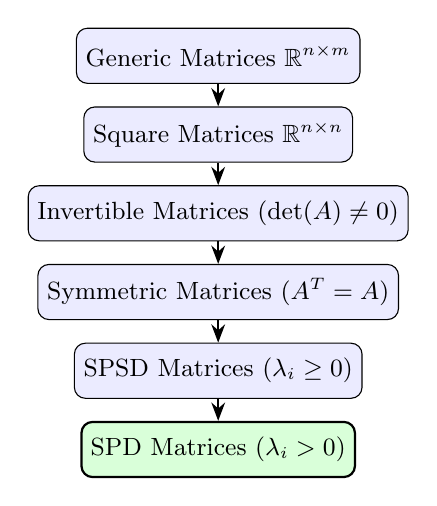
\begin{tikzpicture}[>=Stealth,
    block/.style={rectangle, draw, rounded corners, fill=blue!8, minimum height=0.7cm, font=\small}]
    \node[block] (gen) at (0, 0) {Generic Matrices $\R^{n \times m}$};
    \node[block] (sq) at (0, -1.0) {Square Matrices $\R^{n \times n}$};
    \node[block] (inv) at (0, -2.0) {Invertible Matrices ($\det(A) \neq 0$)};
    \node[block] (sym) at (0, -3.0) {Symmetric Matrices ($A^T = A$)};
    \node[block] (spsd) at (0, -4.0) {SPSD Matrices ($\lambda_i \ge 0$)};
    \node[block, fill=green!15, thick] (spd) at (0, -5.0) {SPD Matrices ($\lambda_i > 0$)};

    \draw[->, thick] (gen) -- (sq);
    \draw[->, thick] (sq) -- (inv);
    \draw[->, thick] (inv) -- (sym);
    \draw[->, thick] (sym) -- (spsd);
    \draw[->, thick] (spsd) -- (spd);
\end{tikzpicture}
\caption{Structural hierarchy and progressive refinement of matrix classes in linear algebra.}
\label{fig:matrix-hierarchy}
\end{figure}

The inclusion is strict:
\begin{equation}
    \text{SPD} \subset \text{SPSD} \subset \text{Symmetric}.
\end{equation}
An SPSD matrix belongs to the SPD class if and only if it is non-singular, meaning it has no zero eigenvalue ($\lambda_{\min} > 0 \iff \det(A) = \prod_{i=1}^n \lambda_i > 0$).

\subsection{Illustrative Examples in \texorpdfstring{$\R^{2 \times 2}$}{R\textasciicircum(2x2)}}

\begin{example}[Verification of SPD and SPSD Matrices]
\mbox{}\par\nopagebreak
\begin{enumerate}
    \item \textbf{SPD Examples:}
    \begin{itemize}
        \item $A_1 = \begin{bmatrix} 1 & 0 \\ 0 & 2 \end{bmatrix}$: symmetric diagonal with eigenvalues $\lambda_1 = 1 > 0, \lambda_2 = 2 > 0 \implies \mathbf{SPD}$.
        \item $A_2 = \begin{bmatrix} 2 & 1 \\ 1 & 2 \end{bmatrix}$: symmetric with eigenvalues calculated in Example~\ref{ex:eigenvalues-2x2} as $\lambda_1 = 3 > 0, \lambda_2 = 1 > 0 \implies \mathbf{SPD}$.
    \end{itemize}
    \item \textbf{SPSD but Non-SPD Examples:}
    \begin{itemize}
        \item $A_3 = \begin{bmatrix} 1 & 0 \\ 0 & 0 \end{bmatrix}$: symmetric diagonal with eigenvalues $\lambda_1 = 1 \ge 0, \lambda_2 = 0 \ge 0 \implies \mathbf{SPSD}$. It is not SPD because $\det(A_3) = 0$.
        \item $A_4 = \begin{bmatrix} 1 & 1 \\ 1 & 1 \end{bmatrix}$: rows are identical, so $\rank(A_4) = 1 < 2$, implying $\lambda_1 = 0$. Because the trace equals the sum of eigenvalues, $\trace(A_4) = 1 + 1 = 2 \implies \lambda_1 + \lambda_2 = 2 \implies \lambda_2 = 2 \ge 0$. The eigenvalues are $\{2, 0\} \implies \mathbf{SPSD}$.
    \end{itemize}
    \item \textbf{Counterexample of an Indefinite Matrix:}
    Consider $A_5 = \begin{bmatrix} 1 & 2 \\ 2 & 0 \end{bmatrix}$. Although its diagonal entries are non-negative, the determinant evaluates to:
    \begin{equation}
        \det(A_5) = 1(0) - 2(2) = -4 < 0.
    \end{equation}
    Because $\det(A_5) = \lambda_1 \lambda_2 = -4 < 0$, the eigenvalues have opposite signs ($\lambda_1 > 0$ and $\lambda_2 < 0$). The matrix is \textbf{indefinite} (neither SPD nor SPSD).
\end{enumerate}
\end{example}

\FloatBarrier
\section[Natural Generation of SPSD Matrices]{Natural Generation of SPSD Matrices: \texorpdfstring{$B^T B$}{B\textasciicircum T B} and \texorpdfstring{$B B^T$}{B B\textasciicircum T}}

In scientific computing and statistics, positive semidefinite matrices are rarely assembled manually; rather, they arise naturally from multiplying a rectangular matrix by its transpose.

\begin{proposition}[Positive Semidefiniteness of Gram Matrices]
\label{prop:btb-bbt-spsd-en}
Let $B \in \R^{n \times m}$ be an arbitrary matrix (square or rectangular). Then:
\begin{enumerate}
    \item The square matrix $B^T B \in \R^{m \times m}$ is symmetric positive semi-definite (\textbf{SPSD}).
    \item The square matrix $B B^T \in \R^{n \times n}$ is symmetric positive semi-definite (\textbf{SPSD}).
\end{enumerate}
\end{proposition}

\begin{proof}
We establish symmetry and positive semidefiniteness:

\medskip
\noindent\textbf{1. Verification of Symmetry:}
Using the transpose of a matrix product:
\begin{equation}
    (B^T B)^T = B^T (B^T)^T = B^T B, \qquad (B B^T)^T = (B^T)^T B^T = B B^T.
\end{equation}
Both matrices are formally symmetric.

\medskip
\noindent\textbf{2. Positive Semidefiniteness of $B^T B$:}
Let $\mathbf{v} \in \R^m$ be an arbitrary vector. Consider the quadratic form:
\begin{equation}
    \mathbf{v}^T (B^T B) \mathbf{v} = (\mathbf{v}^T B^T)(B \mathbf{v}) = (B \mathbf{v})^T (B \mathbf{v}).
\end{equation}
Recognizing the inner product $(B\mathbf{v})^T (B\mathbf{v})$ as the squared Euclidean norm of $\mathbf{w} = B\mathbf{v} \in \R^n$:
\begin{equation}
    \mathbf{v}^T (B^T B) \mathbf{v} = \|B \mathbf{v}\|_2^2.
\end{equation}
By non-negativity of vector norms, $\|B \mathbf{v}\|_2^2 \ge 0$ for all $\mathbf{v} \in \R^m$. Therefore:
\begin{equation}
    \mathbf{v}^T (B^T B) \mathbf{v} \ge 0 \quad \forall \mathbf{v} \in \R^m \implies B^T B \text{ is SPSD}.
\end{equation}

\medskip
\noindent\textbf{3. Positive Semidefiniteness of $B B^T$:}
Let $\mathbf{u} \in \R^n$ be an arbitrary vector. In an identical manner:
\begin{equation}
    \mathbf{u}^T (B B^T) \mathbf{u} = (\mathbf{u}^T B)(B^T \mathbf{u}) = (B^T \mathbf{u})^T (B^T \mathbf{u}) = \|B^T \mathbf{u}\|_2^2 \ge 0 \quad \forall \mathbf{u} \in \R^n.
\end{equation}
Hence $B B^T$ is also SPSD.
\end{proof}

\begin{corollary}[Condition for Strict Positive Definiteness of $B^T B$]
The matrix $B^T B \in \R^{m \times m}$ is \textbf{strictly positive definite (SPD)} if and only if $B$ has full column rank:
\begin{equation}
    B^T B \in \text{SPD} \iff \rank(B) = m \iff \ker(B) = \{\mathbf{0}\}.
\end{equation}
\end{corollary}

\begin{proof}
From the previous proof, $\mathbf{v}^T (B^T B) \mathbf{v} = \|B\mathbf{v}\|_2^2$. This quantity vanishes if and only if $\|B\mathbf{v}\|_2 = 0 \iff B\mathbf{v} = \mathbf{0} \iff \mathbf{v} \in \ker(B)$.
When $\ker(B) = \{\mathbf{0}\}$, no non-zero vector can zero out the quadratic form, making $B^T B$ strictly positive definite.
\end{proof}

\begin{noteblock}{Relevance to Normal Equations and SVD}
This fundamental property underpins two cornerstones of computational mathematics:
\begin{enumerate}
    \item \textbf{Linear Least Squares:} Solving $\min_{\mathbf{x}} \|A\mathbf{x} - \mathbf{b}\|_2$ yields the normal equations:
    \begin{equation}
        A^T A \mathbf{x} = A^T \mathbf{b}.
    \end{equation}
    When $A$ has full column rank, $A^T A$ is SPD, guaranteeing unique solvability via Cholesky factorization.
    \item \textbf{Singular Value Decomposition (SVD):} The singular values $\sigma_i$ of an arbitrary matrix $B$ are defined as the non-negative square roots of the eigenvalues of the SPSD matrix $B^T B$:
    \begin{equation}
        \sigma_i = \sqrt{\lambda_i(B^T B)} \ge 0.
    \end{equation}
\end{enumerate}
\end{noteblock}

\clearpage
\section{Chapter Summary Formulary}

Table~\ref{tab:lecture-3-summary} provides an organized summary of definitions, matrix structures, and algebraic properties covered in this chapter.

\begin{table}[H]
\centering
\resizebox{\textwidth}{!}{%
\begin{tabular}{l l l}
\toprule
\textbf{Concept / Matrix} & \textbf{Mathematical Formulation} & \textbf{Key Property / Spectrum} \\
\midrule
Orthonormal Columns ($k < n$) & $V \in \R^{n \times k}, \; \mathbf{v}_i^T \mathbf{v}_j = \delta_{ij}$ & $V^T V = I_k$, while $V V^T \neq I_n$ \\
Orthogonal Projector & $P = V V^T = \sum_{i=1}^k \mathbf{v}_i \mathbf{v}_i^T$ & Symmetric ($P^T = P$), idempotent ($P^2 = P$), $\rank(P) = k$ \\
Partial Isometry & $\|V\mathbf{x}\|_2 = \|\mathbf{x}\|_2 \quad (\forall \mathbf{x} \in \R^k)$ & Does not preserve norm on $\R^n$: $\|V^T \tilde{\mathbf{y}}\|_2 = 0$ for $\tilde{\mathbf{y}} \in \ker(V^T)$ \\
Eigenpair & $A\mathbf{v} = \lambda \mathbf{v}, \quad \mathbf{v} \neq \mathbf{0}$ & $\lambda$ root of $\det(A - \lambda I_n) = 0$ \\
Diagonalization & $A = V D V^{-1}$ & Requires $n$ linearly independent eigenvectors \\
Dyadic Expansion & $A = \sum_{i=1}^n \lambda_i \mathbf{v}_i \mathbf{w}_i^T$ & Linear combination of $n$ rank-1 matrices \\
Matrix Power & $A^k = V D^k V^{-1}$ & Eigenpairs $(\lambda_i^k, \mathbf{v}_i)$: eigenvectors unchanged \\
Spectral Theorem & $A^T = A \implies A = U D U^T$ & Real eigenvalues, orthonormal eigenvectors ($U^T U = I_n$) \\
Rayleigh Inequality & $\lambda_{\min} \|\mathbf{x}\|_2^2 \le \mathbf{x}^T A \mathbf{x} \le \lambda_{\max} \|\mathbf{x}\|_2^2$ & Bounds attained on corresponding eigenspaces \\
SPD Matrix & $A^T = A, \; \mathbf{x}^T A \mathbf{x} > 0 \; (\forall \mathbf{x} \neq \mathbf{0})$ & All $\lambda_i > 0$; invertible with $\det(A) > 0$ \\
SPSD Matrix & $A^T = A, \; \mathbf{x}^T A \mathbf{x} \ge 0 \; (\forall \mathbf{x})$ & All $\lambda_i \ge 0$; may have zero eigenvalues \\
Gramians $B^T B$ and $B B^T$ & $\mathbf{v}^T (B^T B) \mathbf{v} = \|B\mathbf{v}\|_2^2 \ge 0$ & Always SPSD for any $B \in \R^{n \times m}$ \\
\bottomrule
\end{tabular}%
}
\caption{Comprehensive overview of spectral properties, orthogonal projectors, and quadratic forms.}
\label{tab:lecture-3-summary}
\end{table}

\chapter[Singular Value Decomposition (SVD)]{Singular Value Decomposition (SVD): Theory, Geometry, and Applications}
\label{chap:singular-value-decomposition-svd}

This chapter opens the advanced monograph on modern numerical linear algebra by introducing the \textbf{Singular Value Decomposition} (SVD). After outlining the overarching framework of computational methods (matrix factorizations, linear systems, least-squares problems, eigenvalue algorithms, and floating-point stability), we formalize the SVD in both its extended (\textit{Full SVD}) and compact (\textit{Thin SVD}) formulations. We then develop the rigorous constructive derivation based on the spectral decomposition of the associated symmetric positive semidefinite Gram matrices $A^T A$ and $A A^T$. Finally, we analyze the structure of the four fundamental subspaces and study a series of theoretical and applied problems central to data science and machine learning~\cite{golub2013matrix,trefethen1997numerical,strang2019linear}.

\FloatBarrier
\section{Overview of Numerical Linear Algebra and Lecture Outline}
\label{sec:svd-overview-outline-en}

Numerical linear algebra forms the computational backbone of data science, scientific computing, and optimization~\cite{demmel1997applied,trefethen1997numerical}. In practical engineering and machine learning workflows, physical and statistical models rarely present themselves in closed scalar forms: they almost invariably translate into large-scale matrix operations. This monograph focuses on six essential algorithmic pillars:

\begin{enumerate}
    \item \textbf{Singular Value Decomposition (SVD):} the paramount foundational tool for the spectral analysis of general, rectangular, and rank-deficient matrices. It identifies optimal orthonormal coordinate bases for domain and codomain, quantifies numerical rank, and provides the best low-rank approximation via the Eckart-Young-Mirsky Theorem.

    \item \textbf{QR Factorization:} decomposes any matrix $A \in \R^{n \times m}$ into $A = QR$, where $Q$ has orthonormal columns and $R$ is upper triangular. It guarantees unconditional numerical stability in solving linear least-squares problems and serves as the core iterative engine for computing eigenvalues.

    \item \textbf{Numerical Methods for Linear Systems ($A\mathbf{x} = \mathbf{b}$):}
    \begin{itemize}
        \item \textbf{General formulation:} given a coefficient matrix $A \in \R^{n \times n}$ and a right-hand side vector $\mathbf{b} \in \R^n$, compute the unknown vector $\mathbf{x} \in \R^n$.
        \item \textbf{Direct Methods:} based on triangular or orthogonal factorizations ($LU$, Cholesky $LL^T$, $QR$). In exact arithmetic, they yield the exact solution in a finite, deterministic sequence of steps (with typical complexity $\BigO{n^3}$).
        \item \textbf{Iterative Methods:} suited for sparse matrices of very high dimension ($n \gg 10^5$). They generate successive approximations $\{\mathbf{x}^{(k)}\}_{k \ge 0}$ from an initial guess $\mathbf{x}^{(0)}$, stopping once the relative residual $\|\mathbf{b} - A\mathbf{x}^{(k)}\|_2 / \|\mathbf{b}\|_2$ drops below a preset tolerance $\epsilon_{\text{tol}}$.
    \end{itemize}

    \item \textbf{Numerical Methods for Least-Squares Problems:}
    \begin{equation}
        \min_{\mathbf{x} \in \R^m} \|A\mathbf{x} - \mathbf{b}\|_2,
    \end{equation}
    where $A \in \R^{n \times m}$ is typically overdetermined ($n > m$, geometrically ``tall and thin'') and $\mathbf{b} \in \R^n$. Both direct formulations (normal equations $A^T A \mathbf{x} = A^T \mathbf{b}$, $QR$, SVD) and iterative formulations are examined.

    \item \textbf{Numerical Methods for Eigenvalues and Eigenvectors:} specialized algorithms for the secular problem $A\mathbf{v} = \lambda \mathbf{v}$, including power iteration, inverse iteration, deflation, and the shifted QR algorithm.

    \item \textbf{Conditioning and Numerical Stability:}
    \begin{itemize}
        \item \textbf{Finite precision arithmetic:} standard modern computing uses the IEEE 754 standard for 64-bit floating-point arithmetic (double precision), introducing at each elementary operation a relative roundoff error bounded by the machine epsilon:
        \begin{equation}
            \epsilon_{\text{mach}} = 2^{-53} \approx 1.11 \times 10^{-16}.
        \end{equation}
        \item \textbf{Problem sensitivity vs algorithmic instability:} we formally investigate whether error accumulation stems from the intrinsic sensitivity of the mathematical model to input data perturbations (quantified by the \textit{condition number} $\kappa(A)$) or from destructive error propagation inside the chosen algorithmic scheme.
    \end{itemize}
\end{enumerate}

\begin{alertblock}{Guiding Principle of Numerical Linear Algebra}
An algorithm that is mathematically exact in exact arithmetic may become completely useless on a digital computer if it is not numerically stable. The systematic use of orthogonal matrices (which preserve Euclidean lengths) is the primary line of defense against catastrophic roundoff amplification.
\end{alertblock}

\begin{noteblock}{Reference to Numerical Foundations (Chapter~\ref{chap:computational-models})}
The fundamentals of floating-point error propagation, the definition of the matrix condition number $\kappa(A)$, and the golden rule forbidding the explicit formation of normal equations $A^T A$ (because $\kappa(A^T A) = \kappa(A)^2$) were established in Chapter~\ref{chap:computational-models} at page~\pageref{rem:en:golden-rule-normal-equations}. In this chapter, the SVD provides the ultimate canonical tool for solving least-squares problems while bypassing this catastrophic ill-conditioning.
\end{noteblock}

\FloatBarrier
\section{Definition of the Singular Value Decomposition (Full SVD)}
\label{sec:svd-definition-full-en}

The spectral decomposition for symmetric matrices discussed in the previous chapter ($A = QDQ^T$) suffers from an insurmountable structural limitation: it strictly requires the matrix to be square and symmetric. The Singular Value Decomposition completely overcomes this limitation, extending the concepts of eigenvalues and orthonormal coordinate systems to \textbf{any real matrix of arbitrary dimensions}.

\subsection{Formal Mathematical Definition}

\begin{definition}[Full Singular Value Decomposition (Full SVD)]
\label{def:full-svd-en}
Let $A \in \R^{n \times m}$ be an arbitrary real matrix. A \textbf{Singular Value Decomposition (Full SVD)} of $A$ is a factorization of the form:
\begin{equation}
    A = U \Sigma V^T,
\end{equation}
where the three factors satisfy the following rigorous properties:
\begin{enumerate}
    \item $U \in \R^{n \times n}$ is a square orthogonal matrix:
    \begin{equation}
        U^T U = U U^T = I_n.
    \end{equation}
    The columns of $U = [\mathbf{u}_1, \mathbf{u}_2, \dots, \mathbf{u}_n]$, with $\mathbf{u}_i \in \R^n$, are called \textbf{left singular vectors} and form an orthonormal basis of $\R^n$.

    \item $V \in \R^{m \times m}$ is a square orthogonal matrix:
    \begin{equation}
        V^T V = V V^T = I_m.
    \end{equation}
    The columns of $V = [\mathbf{v}_1, \mathbf{v}_2, \dots, \mathbf{v}_m]$, with $\mathbf{v}_j \in \R^m$, are called \textbf{right singular vectors} and form an orthonormal basis of $\R^m$.

    \item $\Sigma \in \R^{n \times m}$ is a rectangular diagonal matrix matching the dimensions of $A$, whose only non-zero entries may lie on the main diagonal:
    \begin{equation}
        \Sigma_{ii} = \sigma_i \quad \text{for } i = 1, \dots, \min\{n, m\}, \qquad \Sigma_{ij} = 0 \quad \text{if } i \neq j.
    \end{equation}
    The scalars $\sigma_i$ are called \textbf{singular values} of $A$ and satisfy non-negativity and descending order:
    \begin{equation}
        \sigma_1 \ge \sigma_2 \ge \dots \ge \sigma_{\min\{n, m\}} \ge 0.
    \end{equation}
\end{enumerate}
\end{definition}

\subsection{Geometric and Algebraic Meaning of Orthogonality}

The orthogonality of $U$ and $V$ ensures that their columns are pairwise orthonormal under the standard Euclidean inner product:
\begin{equation}
    \langle \mathbf{u}_i, \mathbf{u}_j \rangle = \mathbf{u}_i^T \mathbf{u}_j = \delta_{ij}, \qquad \langle \mathbf{v}_i, \mathbf{v}_j \rangle = \mathbf{v}_i^T \mathbf{v}_j = \delta_{ij}.
\end{equation}
Geometrically, the action of $A$ on an input vector $\mathbf{x} \in \R^m$ decomposes into a sequence of three canonical linear transformations:
\begin{equation}
    \mathbf{x} \;\xrightarrow{\quad V^T \quad}\; \tilde{\mathbf{x}} = V^T \mathbf{x} \;\xrightarrow{\quad \Sigma \quad}\; \tilde{\mathbf{y}} = \Sigma \tilde{\mathbf{x}} \;\xrightarrow{\quad U \quad}\; \mathbf{y} = U \tilde{\mathbf{y}} = A\mathbf{x}.
\end{equation}
\begin{itemize}
    \item \textbf{Rotation / reflection in $\R^m$ ($V^T$):} the vector $\mathbf{x}$ is projected onto the orthonormal coordinate system formed by the right singular vectors $\{\mathbf{v}_j\}$. Because $V$ is orthogonal, this preserves Euclidean norms ($\|V^T \mathbf{x}\|_2 = \|\mathbf{x}\|_2$).
    \item \textbf{Coordinate stretching ($\Sigma$):} each coordinate is scaled independently by the corresponding singular value $\sigma_i$. When dimensions differ ($n \neq m$), $\Sigma$ also performs embedding or dimension reduction.
    \item \textbf{Rotation / reflection in $\R^n$ ($U$):} the scaled vector is rotated into the codomain $\R^n$ along the orthonormal system of the left singular vectors $\{\mathbf{u}_i\}$.
\end{itemize}

\subsection{Block Structure of \texorpdfstring{$\Sigma$}{Sigma} and Matrix Morphology}

Depending on the relationship between $n$ and $m$, the matrix $\Sigma \in \R^{n \times m}$ takes one of three canonical block forms:

\begin{enumerate}
    \item \textbf{Square Matrix Case ($n = m$):}
    All factors are $n \times n$. The matrix $\Sigma$ is purely diagonal:
    \begin{equation}
        \Sigma = \begin{bmatrix}
            \sigma_1 & & 0 \\
            & \ddots & \\
            0 & & \sigma_n
        \end{bmatrix} \in \R^{n \times n}.
    \end{equation}

    \item \textbf{Short and Wide Matrix Case ($n < m$):}
    Underdetermined system (fewer constraints than variables). $U \in \R^{n \times n}$ is small and square, while $V \in \R^{m \times m}$ is large and square. $\Sigma$ partitions into an $n \times n$ diagonal block followed by a zero block:
    \begin{equation}
        \Sigma = \begin{bmatrix} \Sigma_1 & 0_{n \times (m - n)} \end{bmatrix} = \begin{bmatrix}
            \sigma_1 & & 0 & 0 & \dots & 0 \\
            & \ddots & & \vdots & \ddots & \vdots \\
            0 & & \sigma_n & 0 & \dots & 0
        \end{bmatrix} \in \R^{n \times m},
    \end{equation}
    with $\Sigma_1 = \diag(\sigma_1, \dots, \sigma_n) \in \R^{n \times n}$.

    \item \textbf{Tall and Thin Matrix Case ($n > m$):}
    Overdetermined system typical of data fitting ($n$ samples, $m$ features). $U \in \R^{n \times n}$ is large and square, while $V \in \R^{m \times m}$ is small and square. $\Sigma$ partitions vertically into an $m \times m$ diagonal block and a bottom zero block of size $(n - m) \times m$:
    \begin{equation}
        \Sigma = \begin{bmatrix} \Sigma_1 \\ 0_{(n - m) \times m} \end{bmatrix} = \begin{bmatrix}
            \sigma_1 & & 0 \\
            & \ddots & \\
            0 & & \sigma_m \\
            0 & \dots & 0 \\
            \vdots & \ddots & \vdots \\
            0 & \dots & 0
        \end{bmatrix} \in \R^{n \times m},
    \end{equation}
    with $\Sigma_1 = \diag(\sigma_1, \dots, \sigma_m) \in \R^{m \times m}$.
\end{enumerate}

\subsection{Dyadic Form (Outer Product Expansion)}

Recall the general column-partitioned matrix product: given $B = [\mathbf{b}_1, \dots, \mathbf{b}_k]$ and $C = [\mathbf{c}_1, \dots, \mathbf{c}_k]$, their product expands into a sum of $k$ rank-one outer products:
\begin{equation}
    B C^T = \sum_{j=1}^k \mathbf{b}_j \mathbf{c}_j^T.
\end{equation}
Applying this to the SVD factorization, because $\Sigma$ simply multiplies the $j$-th column of $U$ by the scalar $\sigma_j$, the linear operator $A$ can be written compactly as:
\begin{equation}
\label{eq:svd-dyadic-form-en}
    A = \sum_{j=1}^{\min\{n, m\}} \sigma_j \mathbf{u}_j \mathbf{v}_j^T = \sigma_1 \mathbf{u}_1 \mathbf{v}_1^T + \sigma_2 \mathbf{u}_2 \mathbf{v}_2^T + \dots + \sigma_p \mathbf{u}_p \mathbf{v}_p^T,
\end{equation}
where $p = \min\{n, m\}$. Each term $\mathbf{u}_j \mathbf{v}_j^T \in \R^{n \times m}$ is an \textbf{orthonormal rank-one matrix}. The dyadic expansion therefore decomposes $A$ into a weighted sum of rank-one structures, where the weights are the non-increasing singular values $\sigma_j \ge 0$.

\FloatBarrier
\section{Existence and Construction of the SVD}
\label{sec:svd-existence-construction-en}

\subsection{Fundamental Existence Theorem}

\begin{theorem}[Global Existence of the SVD]
\label{thm:existence-svd-en}
For every real matrix $A \in \R^{n \times m}$, of arbitrary dimensions and arbitrary rank, there exist two orthogonal matrices $U \in \R^{n \times n}$ and $V \in \R^{m \times m}$ and a rectangular diagonal matrix $\Sigma \in \R^{n \times m}$ with ordered non-negative diagonal elements $\sigma_1 \ge \sigma_2 \ge \dots \ge \sigma_{\min\{n,m\}} \ge 0$ such that:
\begin{equation}
    A = U \Sigma V^T.
\end{equation}
\end{theorem}

\subsection{Constructive Derivation via Reverse Engineering}

To reveal where $U, \Sigma, V$ naturally arise, consider a constructive reverse-engineering strategy. Assume tentatively that the factorization $A = U \Sigma V^T$ exists, and compute the associated symmetric Gram matrix $A^T A \in \R^{m \times m}$:
\begin{align}
    A^T A &= (U \Sigma V^T)^T (U \Sigma V^T) \nonumber \\
          &= (V \Sigma^T U^T)(U \Sigma V^T) \nonumber \\
          &= V \Sigma^T (U^T U) \Sigma V^T.
\end{align}
Because $U$ is orthogonal, $U^T U = I_n$. Hence:
\begin{equation}
    A^T A = V (\Sigma^T \Sigma) V^T.
\end{equation}
When $n = m$, $\Sigma$ is square and diagonal ($\Sigma^T = \Sigma$), which yields $\Sigma^T \Sigma = \Sigma^2 = \diag(\sigma_1^2, \dots, \sigma_n^2)$. 
The identity:
\begin{equation}
    A^T A = V \Sigma^2 V^T
\end{equation}
matches exactly the \textbf{spectral decomposition} of the real symmetric matrix $A^T A$. This yields two crucial insights:
\begin{itemize}
    \item The columns of $V$ must be the orthonormal eigenvectors of $A^T A$.
    \item The squared singular values $\sigma_j^2$ of $A$ must equal the eigenvalues of $A^T A$:
    \begin{equation}
        \lambda_j(A^T A) = \sigma_j^2 \implies \sigma_j = \sqrt{\lambda_j(A^T A)}.
    \end{equation}
\end{itemize}

Symmetrically, computing $A A^T \in \R^{n \times n}$:
\begin{equation}
    A A^T = (U \Sigma V^T)(V \Sigma^T U^T) = U (\Sigma \Sigma^T) U^T = U \Sigma^2 U^T,
\end{equation}
we see that the columns of $U$ are the orthonormal eigenvectors of $A A^T$.

\subsection{Rigorous Proof for Square Invertible Matrices}

We now prove Theorem~\ref{thm:existence-svd-en} constructively in the case where $A \in \R^{n \times n}$ is square and non-singular ($\det(A) \neq 0$).

\begin{proof}
The proof proceeds in five structured steps:

\paragraph{Step 1: Algebraic properties of $A^T A$.}
Let $M = A^T A \in \R^{n \times n}$.
\begin{enumerate}
    \item $M$ is symmetric: $M^T = (A^T A)^T = A^T A = M$.
    \item $M$ is symmetric positive definite (SPD). Indeed, for any non-zero $\mathbf{x} \in \R^n \setminus \{\mathbf{0}\}$:
    \begin{equation}
        \mathbf{x}^T M \mathbf{x} = \mathbf{x}^T (A^T A) \mathbf{x} = (A\mathbf{x})^T (A\mathbf{x}) = \|A\mathbf{x}\|_2^2.
    \end{equation}
    Since $A$ is invertible by hypothesis, $\ker(A) = \{\mathbf{0}\}$; thus $\mathbf{x} \neq \mathbf{0} \implies A\mathbf{x} \neq \mathbf{0}$, which gives $\|A\mathbf{x}\|_2^2 > 0$.
\end{enumerate}

\paragraph{Step 2: Spectral decomposition of $A^T A$.}
Since $A^T A$ is real, symmetric, and positive definite, the Spectral Theorem yields an orthogonal matrix $Q \in \R^{n \times n}$ ($Q^T Q = I_n$) and a diagonal matrix $D \in \R^{n \times n}$ such that:
\begin{equation}
    A^T A = Q D Q^T,
\end{equation}
where the eigenvalues along the diagonal of $D$ are strictly positive and sorted non-increasingly:
\begin{equation}
    D = \begin{bmatrix}
        d_1 & & 0 \\
        & \ddots & \\
        0 & & d_n
    \end{bmatrix}, \qquad d_1 \ge d_2 \ge \dots \ge d_n > 0.
\end{equation}

\paragraph{Step 3: Definition of factors $V$ and $\Sigma$.}
Following the reverse-engineering derivation, define:
\begin{align}
    V &:= Q \in \R^{n \times n} \quad (\implies V \text{ is orthogonal: } V^T V = I_n), \\
    \Sigma &:= D^{1/2} = \begin{bmatrix}
        \sqrt{d_1} & & 0 \\
        & \ddots & \\
        0 & & \sqrt{d_n}
    \end{bmatrix} \in \R^{n \times n}.
\end{align}
Because each $d_j > 0$, the quantities $\sigma_j := \sqrt{d_j}$ are well-defined, strictly positive real numbers:
\begin{equation}
    \sigma_1 \ge \sigma_2 \ge \dots \ge \sigma_n > 0.
\end{equation}

\paragraph{Step 4: Algebraic formulation of matrix $U$.}
Requiring the factorization $A = U \Sigma V^T$ to hold, substitute our defined factors:
\begin{equation}
    A = U D^{1/2} Q^T.
\end{equation}
Multiplying both sides on the right by $Q$ and using $Q^T Q = I_n$:
\begin{equation}
    A Q = U D^{1/2}.
\end{equation}
Since all diagonal entries of $D^{1/2}$ are strictly positive ($\sigma_j > 0$), $D^{1/2}$ is invertible with:
\begin{equation}
    D^{-1/2} = \begin{bmatrix}
        \frac{1}{\sqrt{d_1}} & & 0 \\
        & \ddots & \\
        0 & & \frac{1}{\sqrt{d_n}}
    \end{bmatrix}.
\end{equation}
Hence, we can solve for $U$:
\begin{equation}
\label{eq:svd-construct-U-en}
    U := A Q D^{-1/2}.
\end{equation}

\paragraph{Step 5: Verifying the orthogonality of $U$.}
We must confirm that $U$ is orthogonal, namely $U^T U = I_n$.
Evaluating the product explicitly:
\begin{align}
    U^T U &= \left( A Q D^{-1/2} \right)^T \left( A Q D^{-1/2} \right) \nonumber \\
          &= \left( D^{-1/2} \right)^T Q^T A^T A Q D^{-1/2}.
\end{align}
Because $D^{-1/2}$ is diagonal, $(D^{-1/2})^T = D^{-1/2}$. Substituting $A^T A = Q D Q^T$:
\begin{align}
    U^T U &= D^{-1/2} Q^T (Q D Q^T) Q D^{-1/2} \nonumber \\
          &= D^{-1/2} (Q^T Q) D (Q^T Q) D^{-1/2}.
\end{align}
Since $Q$ is orthogonal ($Q^T Q = I_n$):
\begin{align}
    U^T U &= D^{-1/2} I_n D I_n D^{-1/2} \nonumber \\
          &= D^{-1/2} D D^{-1/2}.
\end{align}
Multiplying the diagonal matrices entry by entry:
\begin{equation}
    D^{-1/2} D D^{-1/2} = \begin{bmatrix}
        \frac{1}{\sqrt{d_1}} \cdot d_1 \cdot \frac{1}{\sqrt{d_1}} & & 0 \\
        & \ddots & \\
        0 & & \frac{1}{\sqrt{d_n}} \cdot d_n \cdot \frac{1}{\sqrt{d_n}}
    \end{bmatrix} = \begin{bmatrix}
        \frac{d_1}{d_1} & & 0 \\
        & \ddots & \\
        0 & & \frac{d_n}{d_n}
    \end{bmatrix} = I_n.
\end{equation}
Since $U \in \R^{n \times n}$ is square and satisfies $U^T U = I_n$, it follows that $U$ is orthogonal ($U U^T = I_n$). The theorem is proved for invertible square matrices.
\end{proof}

\subsection{Extension to General Rectangular or Deficient Matrices}

When $A \in \R^{n \times m}$ is rectangular or square singular, the symmetric matrix $A^T A \in \R^{m \times m}$ is only \textbf{positive semidefinite} (SPSD).
Let $r = \rank(A) = \rank(A^T A) \le \min\{n, m\}$. The eigenvalues of $A^T A$ partition into:
\begin{equation}
    d_1 \ge d_2 \ge \dots \ge d_r > d_{r+1} = \dots = d_m = 0.
\end{equation}
Consequently, $D$ contains zero entries and the global inverse $D^{-1/2}$ does not exist. We therefore construct $U$ \textbf{column by column}:
\begin{enumerate}
    \item For indices with positive singular values ($j = 1, \dots, r$), define:
    \begin{equation}
        \mathbf{u}_j := \frac{1}{\sqrt{d_j}} A \mathbf{q}_j = \frac{1}{\sigma_j} A \mathbf{v}_j.
    \end{equation}
    These $r$ vectors $\{\mathbf{u}_1, \dots, \mathbf{u}_r\} \subset \R^n$ are orthonormal:
    \begin{equation}
        \mathbf{u}_i^T \mathbf{u}_j = \left(\frac{1}{\sigma_i} A \mathbf{v}_i\right)^T \left(\frac{1}{\sigma_j} A \mathbf{v}_j\right) = \frac{\mathbf{v}_i^T (A^T A) \mathbf{v}_j}{\sigma_i \sigma_j} = \frac{\mathbf{v}_i^T (d_j \mathbf{v}_j)}{\sigma_i \sigma_j} = \frac{d_j \delta_{ij}}{\sigma_i \sigma_j} = \delta_{ij}.
    \end{equation}
    \item If $r < n$, the first $r$ vectors span only an $r$-dimensional subspace in $\R^n$. To form a complete orthonormal basis of $\R^n$, we choose $n - r$ additional orthonormal vectors $\{\mathbf{u}_{r+1}, \dots, \mathbf{u}_n\}$ spanning the orthogonal complement $\operatorname{span}(\mathbf{u}_1, \dots, \mathbf{u}_r)^\perp = \ker(A^T)$, using the Gram-Schmidt orthogonalization process.
\end{enumerate}

\FloatBarrier
\section{Thin SVD vs Full SVD and Computational Profile}
\label{sec:svd-thin-vs-full-en}

In modern data science and machine learning applications, the dimensions of $A \in \R^{n \times m}$ are heavily asymmetric ($n \gg m$, e.g., millions of observations and tens or hundreds of features). In such regimes, storing and computing the Full SVD is impractical.

\subsection{Definition of the Thin SVD (Economy SVD)}

Let $A \in \R^{n \times m}$ be tall and thin ($n > m$). The Full SVD decomposes $A$ as:
\begin{equation}
    A = U \Sigma V^T, \qquad U \in \R^{n \times n}, \quad \Sigma \in \R^{n \times m}, \quad V \in \R^{m \times m}.
\end{equation}
Because $n > m$, the bottom $n - m$ rows of $\Sigma$ are identically zero:
\begin{equation}
    \Sigma = \begin{bmatrix} \Sigma_0 \\ 0_{(n-m) \times m} \end{bmatrix}, \qquad \Sigma_0 = \diag(\sigma_1, \dots, \sigma_m) \in \R^{m \times m}.
\end{equation}
Partitioning the orthogonal matrix $U$ into its first $m$ columns $U_0$ and the remaining $n - m$ columns $U_\perp$:
\begin{equation}
    U = \begin{bmatrix} U_0 & U_\perp \end{bmatrix}, \qquad U_0 \in \R^{n \times m}, \quad U_\perp \in \R^{n \times (n - m)}.
\end{equation}
Performing block multiplication:
\begin{align}
    A &= \begin{bmatrix} U_0 & U_\perp \end{bmatrix} \begin{bmatrix} \Sigma_0 \\ 0 \end{bmatrix} V^T \nonumber \\
      &= \left( U_0 \Sigma_0 + U_\perp \cdot 0 \right) V^T \nonumber \\
      &= U_0 \Sigma_0 V^T.
\end{align}
Notice that the last $n - m$ columns collected in $U_\perp$ are multiplied solely by zeros: \textbf{they provide zero contribution to the reconstruction of $A$}.

\begin{definition}[Thin SVD / Economy SVD]
\label{def:thin-svd-en}
Let $A \in \R^{n \times m}$ with $n \ge m$. The \textbf{Thin SVD} (or economy-size SVD) of $A$ is the factorization:
\begin{equation}
    A = U_0 \Sigma_0 V^T,
\end{equation}
where:
\begin{itemize}
    \item $U_0 \in \R^{n \times m}$ has orthonormal columns ($U_0^T U_0 = I_m$), but is not square ($U_0 U_0^T \neq I_n$; it acts as an orthogonal projector onto $\operatorname{Im}(A)$).
    \item $\Sigma_0 = \diag(\sigma_1, \dots, \sigma_m) \in \R^{m \times m}$ is a square diagonal matrix containing all singular values.
    \item $V \in \R^{m \times m}$ is the standard square orthogonal matrix ($V^T V = V V^T = I_m$).
\end{itemize}
\end{definition}

Both Full SVD and Thin SVD yield the exact same dyadic sum:
\begin{equation}
    A = \sum_{j=1}^m \sigma_j \mathbf{u}_j \mathbf{v}_j^T.
\end{equation}

\begin{figure}[H]
\centering
\resizebox{0.95\textwidth}{!}{%
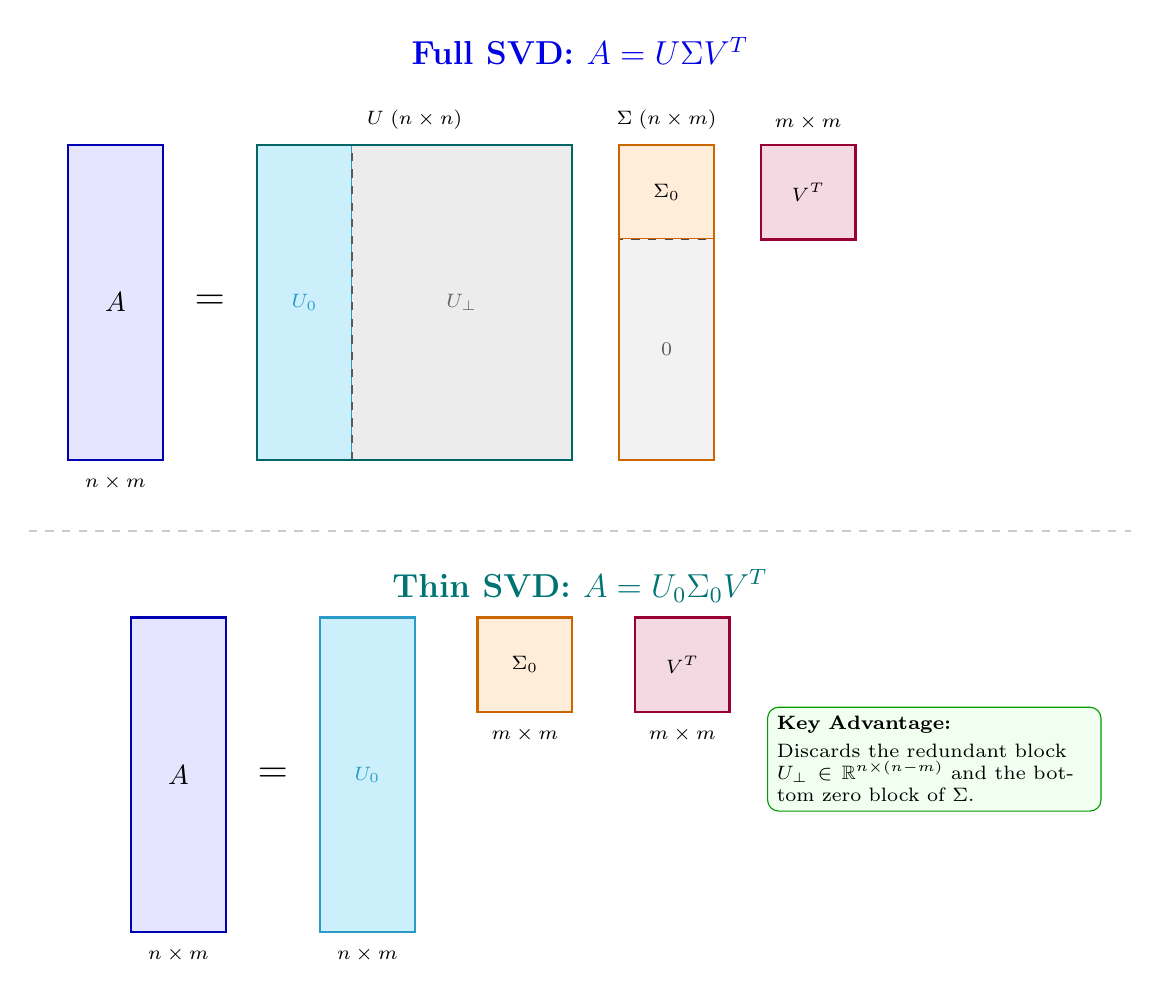
\begin{tikzpicture}[>=Stealth,
    blockA/.style={fill=blue!10, draw=blue!70!black, thick},
    blockU/.style={fill=teal!15, draw=teal!80!black, thick},
    blockUzero/.style={fill=cyan!20, draw=cyan!80!black, thick},
    blockUperp/.style={fill=gray!15, draw=gray!70!black, dashed, thick},
    blockSigma/.style={fill=orange!15, draw=orange!80!black, thick},
    blockSigZero/.style={fill=gray!10, draw=gray!60!black, dashed},
    blockV/.style={fill=purple!15, draw=purple!80!black, thick},
    brace/.style={decorate, decoration={brace, amplitude=4pt, raise=2pt}}
]

    % Full SVD Title
    \node[font=\bfseries\large, text=blue!90!black] at (6.5, 5.2) {Full SVD: $A = U \Sigma V^T$};

    % Matrice A (n x m)
    \draw[blockA] (0, 0) rectangle (1.2, 4.0);
    \node[font=\bfseries] at (0.6, 2.0) {$A$};
    \node[below=2pt, font=\scriptsize] at (0.6, 0) {$n \times m$};

    \node[font=\Large] at (1.8, 2.0) {$=$};

    % Matrice U (n x n)
    \draw[blockUzero] (2.4, 0) rectangle (3.6, 4.0);
    \node[font=\scriptsize\bfseries, text=cyan!80!black] at (3.0, 2.0) {$U_0$};
    \draw[blockUperp] (3.6, 0) rectangle (6.4, 4.0);
    \node[font=\scriptsize\bfseries, text=gray!80!black] at (5.0, 2.0) {$U_\perp$};
    \draw[thick, draw=teal!80!black] (2.4, 0) rectangle (6.4, 4.0);
    \node[above=2pt, font=\scriptsize] at (4.4, 4.0) {$U \; (n \times n)$};

    % Matrice Sigma (n x m)
    \draw[blockSigma] (7.0, 2.8) rectangle (8.2, 4.0);
    \node[font=\scriptsize\bfseries] at (7.6, 3.4) {$\Sigma_0$};
    \draw[blockSigZero] (7.0, 0) rectangle (8.2, 2.8);
    \node[font=\scriptsize, text=gray!70!black] at (7.6, 1.4) {$0$};
    \draw[thick, draw=orange!80!black] (7.0, 0) rectangle (8.2, 4.0);
    \node[above=2pt, font=\scriptsize] at (7.6, 4.0) {$\Sigma \; (n \times m)$};

    % Matrice V^T (m x m)
    \draw[blockV] (8.8, 2.8) rectangle (10.0, 4.0);
    \node[font=\scriptsize\bfseries] at (9.4, 3.4) {$V^T$};
    \node[above=2pt, font=\scriptsize] at (9.4, 4.0) {$m \times m$};

    % Separatore orizzontale
    \draw[thick, gray!40, dashed] (-0.5, -0.9) -- (13.5, -0.9);

    % Thin SVD Title
    \node[font=\bfseries\large, text=teal!90!black] at (6.5, -1.6) {Thin SVD: $A = U_0 \Sigma_0 V^T$};

    % Matrice A (n x m)
    \draw[blockA] (0.8, -6.0) rectangle (2.0, -2.0);
    \node[font=\bfseries] at (1.4, -4.0) {$A$};
    \node[below=2pt, font=\scriptsize] at (1.4, -6.0) {$n \times m$};

    \node[font=\Large] at (2.6, -4.0) {$=$};

    % Matrice U0 (n x m)
    \draw[blockUzero] (3.2, -6.0) rectangle (4.4, -2.0);
    \node[font=\scriptsize\bfseries, text=cyan!80!black] at (3.8, -4.0) {$U_0$};
    \node[below=2pt, font=\scriptsize] at (3.8, -6.0) {$n \times m$};

    % Matrice Sigma0 (m x m)
    \draw[blockSigma] (5.2, -3.2) rectangle (6.4, -2.0);
    \node[font=\scriptsize\bfseries] at (5.8, -2.6) {$\Sigma_0$};
    \node[below=2pt, font=\scriptsize] at (5.8, -3.2) {$m \times m$};

    % Matrice V^T (m x m)
    \draw[blockV] (7.2, -3.2) rectangle (8.4, -2.0);
    \node[font=\scriptsize\bfseries] at (7.8, -2.6) {$V^T$};
    \node[below=2pt, font=\scriptsize] at (7.8, -3.2) {$m \times m$};

    % Notazione risparmio
    \node[draw=green!60!black, fill=green!6, rounded corners=4pt, text width=4.0cm, align=left, font=\scriptsize] at (11.0, -3.8) {
        \textbf{Key Advantage:}\\[2pt]
        Discards the redundant block $U_\perp \in \R^{n \times (n-m)}$ and the bottom zero block of $\Sigma$.
    };

\end{tikzpicture}%
}
\caption{Structural and geometric comparison between Full SVD and Thin SVD for a tall and thin matrix ($n > m$).}
\label{fig:svd-full-vs-thin-en}
\end{figure}

\subsection{Memory and Asymptotic Computational Complexity Comparison}

Table~\ref{tab:svd-full-vs-thin-complexity-en} outlines the computational disparity between Full SVD and Thin SVD when $n \ge m$.

\begin{table}[H]
\centering
\resizebox{0.95\textwidth}{!}{%
\begin{tabular}{l l l}
\toprule
\textbf{Property / Resource} & \textbf{Full SVD ($n \ge m$)} & \textbf{Thin SVD ($n \ge m$)} \\
\midrule
\textbf{Dimension of $U$} & $n \times n$ & $n \times m$ \\
\textbf{Dimension of $\Sigma$} & $n \times m$ & $m \times m$ (square) \\
\textbf{Dimension of $V$} & $m \times m$ & $m \times m$ \\
\textbf{Memory Footprint} & $\BigO{n^2}$ words & $\BigO{nm}$ words \\
\textbf{Asymptotic Complexity} & $\BigO{n^2 m}$ flops & $\BigO{n m^2}$ flops \\
\bottomrule
\end{tabular}%
}
\caption{Asymptotic memory and computational complexity comparison between Full SVD and Thin SVD.}
\label{tab:svd-full-vs-thin-complexity-en}
\end{table}

\begin{example}[Practical Impact in Big Data Analytics]
Consider a data matrix with $n = 10^6$ instances (rows) and $m = 10$ features (columns).
\begin{itemize}
    \item \textbf{Full SVD:} $U$ has size $10^6 \times 10^6$, requiring $10^{12}$ double-precision floats. In terms of RAM:
    \begin{equation}
        10^{12} \times 8 \text{ bytes} = 8 \times 10^{12} \text{ bytes} \approx 8 \text{ TB},
    \end{equation}
    which exceeds standard single-machine memory capacities.
    \item \textbf{Thin SVD:} $U_0$ requires only $n \times m = 10^7$ floats:
    \begin{equation}
        10^7 \times 8 \text{ bytes} = 80 \text{ MB},
    \end{equation}
    which easily fits in memory on any workstation or laptop.
\end{itemize}
Consequently, scientific computing packages (such as \texttt{scipy.linalg.svd(..., full\_matrices=False)} in Python, \texttt{svd(A, 'econ')} in MATLAB, and LAPACK drivers with option \texttt{'S'}) default to or strongly recommend the Thin SVD.
\end{example}

\FloatBarrier
\section{Numerical Rank and the Four Fundamental Subspaces}
\label{sec:svd-four-subspaces-en}

\subsection{Exact Rank Determination via Singular Values}

A profound theoretical and numerical advantage of the SVD is its ability to cleanly determine the rank of a matrix.
Recall the dyadic expansion~\eqref{eq:svd-dyadic-form-en}:
\begin{equation}
    A = \sum_{j=1}^{\min\{n, m\}} \sigma_j \mathbf{u}_j \mathbf{v}_j^T.
\end{equation}
Because the vectors $\{\mathbf{u}_j\}_{j=1}^n$ are orthonormal in $\R^n$ and $\{\mathbf{v}_j\}_{j=1}^m$ are orthonormal in $\R^m$, each term $\mathbf{u}_j \mathbf{v}_j^T$ has rank exactly 1. Furthermore, these rank-one matrices are mutually orthogonal under the Frobenius inner product:
\begin{equation}
    \langle \mathbf{u}_i \mathbf{v}_i^T, \mathbf{u}_j \mathbf{v}_j^T \rangle_F = \trace\left( (\mathbf{u}_i \mathbf{v}_i^T)^T (\mathbf{u}_j \mathbf{v}_j^T) \right) = \trace\left( \mathbf{v}_i \mathbf{u}_i^T \mathbf{u}_j \mathbf{v}_j^T \right) = \delta_{ij} \delta_{ij} = \delta_{ij}.
\end{equation}
This leads to the following proposition:

\begin{proposition}[Rank Characterization via SVD]
The rank of $A \in \R^{n \times m}$ equals the number of strictly positive singular values:
\begin{equation}
    \rank(A) = r \iff \sigma_1 \ge \dots \ge \sigma_r > \sigma_{r+1} = \dots = \sigma_{\min\{n, m\}} = 0.
\end{equation}
Accordingly, the dyadic sum truncates at index $r$:
\begin{equation}
    A = \sum_{j=1}^r \sigma_j \mathbf{u}_j \mathbf{v}_j^T.
\end{equation}
\end{proposition}

\subsection{Characterization of the Four Fundamental Subspaces}

The Full SVD automatically yields orthonormal bases for all four fundamental subspaces associated with $A$ and $A^T$.
To illustrate the algebraic mechanism, consider the classroom case study: a matrix $A \in \R^{6 \times 4}$ ($n = 6, m = 4$) with rank $r = 3$.

Here, $\Sigma$ contains $r = 3$ positive singular values $\sigma_1 \ge \sigma_2 \ge \sigma_3 > 0$ and $\sigma_4 = 0$:
\begin{equation}
    A = \sigma_1 \mathbf{u}_1 \mathbf{v}_1^T + \sigma_2 \mathbf{u}_2 \mathbf{v}_2^T + \sigma_3 \mathbf{u}_3 \mathbf{v}_3^T.
\end{equation}

\paragraph{1. Nullspace of $A$ ($\ker(A) \subseteq \R^4$).}
The nullspace is defined as $\{\mathbf{x} \in \R^4 : A\mathbf{x} = \mathbf{0}\}$. Multiply $A$ by the fourth right singular vector $\mathbf{v}_4$:
\begin{align}
    A \mathbf{v}_4 &= \left( \sigma_1 \mathbf{u}_1 \mathbf{v}_1^T + \sigma_2 \mathbf{u}_2 \mathbf{v}_2^T + \sigma_3 \mathbf{u}_3 \mathbf{v}_3^T \right) \mathbf{v}_4 \nonumber \\
                   &= \sigma_1 \mathbf{u}_1 (\mathbf{v}_1^T \mathbf{v}_4) + \sigma_2 \mathbf{u}_2 (\mathbf{v}_2^T \mathbf{v}_4) + \sigma_3 \mathbf{u}_3 (\mathbf{v}_3^T \mathbf{v}_4).
\end{align}
Since $V$ is orthogonal, its columns are orthonormal: $\mathbf{v}_1^T \mathbf{v}_4 = 0$, $\mathbf{v}_2^T \mathbf{v}_4 = 0$, $\mathbf{v}_3^T \mathbf{v}_4 = 0$. Hence:
\begin{equation}
    A \mathbf{v}_4 = \mathbf{0} \implies \mathbf{v}_4 \in \ker(A).
\end{equation}
By the rank-nullity theorem, $\dim(\ker(A)) = m - r = 4 - 3 = 1$. Since $\|\mathbf{v}_4\|_2 = 1$, it forms an orthonormal basis for the nullspace:
\begin{equation}
    \ker(A) = \spanop\{\mathbf{v}_4\}.
\end{equation}

\paragraph{2. Range / Column Space of $A$ ($\operatorname{Im}(A) \subseteq \R^6$).}
The range is $\{A\mathbf{x} : \mathbf{x} \in \R^4\}$. For any $\mathbf{x} \in \R^4$:
\begin{align}
    A\mathbf{x} &= \sigma_1 \mathbf{u}_1 (\mathbf{v}_1^T \mathbf{x}) + \sigma_2 \mathbf{u}_2 (\mathbf{v}_2^T \mathbf{x}) + \sigma_3 \mathbf{u}_3 (\mathbf{v}_3^T \mathbf{x}) \nonumber \\
                &= (\sigma_1 \mathbf{v}_1^T \mathbf{x}) \mathbf{u}_1 + (\sigma_2 \mathbf{v}_2^T \mathbf{x}) \mathbf{u}_2 + (\sigma_3 \mathbf{v}_3^T \mathbf{x}) \mathbf{u}_3.
\end{align}
Because the scalar coefficients vary arbitrarily over $\R$, every vector $A\mathbf{x}$ is a linear combination of the first three columns of $U$. Since $\{\mathbf{u}_1, \mathbf{u}_2, \mathbf{u}_3\}$ are orthonormal and $\dim(\operatorname{Im}(A)) = r = 3$:
\begin{equation}
    \operatorname{Im}(A) = \spanop\{\mathbf{u}_1, \mathbf{u}_2, \mathbf{u}_3\}.
\end{equation}

\paragraph{3. Range and Nullspace of the Transpose $A^T$.}
Examining the transpose $A^T = (U \Sigma V^T)^T = V \Sigma^T U^T$, the roles of $U$ and $V$ are reversed:
\begin{equation}
    A^T = \sigma_1 \mathbf{v}_1 \mathbf{u}_1^T + \sigma_2 \mathbf{v}_2 \mathbf{u}_2^T + \sigma_3 \mathbf{v}_3 \mathbf{u}_3^T.
\end{equation}
By the exact same reasoning:
\begin{itemize}
    \item \textbf{Range of $A^T$ ($\operatorname{Im}(A^T) \subseteq \R^4$):}
    \begin{equation}
        \operatorname{Im}(A^T) = \spanop\{\mathbf{v}_1, \mathbf{v}_2, \mathbf{v}_3\}.
    \end{equation}
    \item \textbf{Nullspace of $A^T$ ($\ker(A^T) \subseteq \R^6$):}
    multiplying $A^T$ by the remaining left singular vectors $\mathbf{u}_4, \mathbf{u}_5, \mathbf{u}_6$, orthogonality gives $A^T \mathbf{u}_k = \mathbf{0}$ for $k \in \{4, 5, 6\}$. Since $\dim(\ker(A^T)) = n - r = 6 - 3 = 3$:
    \begin{equation}
        \ker(A^T) = \spanop\{\mathbf{u}_4, \mathbf{u}_5, \mathbf{u}_6\}.
    \end{equation}
\end{itemize}

\begin{theorem}[Fundamental Subspaces via SVD]
\label{thm:subspaces-svd-general-en}
Let $A \in \R^{n \times m}$ have SVD $A = U \Sigma V^T$ and rank $r$. The columns of $U$ and $V$ provide orthonormal bases for the four fundamental subspaces:
\begin{enumerate}
    \item $\operatorname{Im}(A) = \spanop\{\mathbf{u}_1, \dots, \mathbf{u}_r\} \subseteq \R^n \quad (\text{dimension } r)$.
    \item $\ker(A^T) = \spanop\{\mathbf{u}_{r+1}, \dots, \mathbf{u}_n\} \subseteq \R^n \quad (\text{dimension } n - r)$.
    \item $\operatorname{Im}(A^T) = \spanop\{\mathbf{v}_1, \dots, \mathbf{v}_r\} \subseteq \R^m \quad (\text{dimension } r)$.
    \item $\ker(A) = \spanop\{\mathbf{v}_{r+1}, \dots, \mathbf{v}_m\} \subseteq \R^m \quad (\text{dimension } m - r)$.
\end{enumerate}
Moreover, orthogonal complement direct sums hold:
\begin{equation}
    \operatorname{Im}(A) \oplus \ker(A^T) = \R^n, \qquad \operatorname{Im}(A^T) \oplus \ker(A) = \R^m.
\end{equation}
\end{theorem}

\FloatBarrier
\section{Theoretical Problems and Worked Applications}
\label{sec:svd-problems-applications-en}

During the interactive classroom problem session [time interval 80:00 - 104:00], students tackle four foundational conceptual problems. The instructor's guidance highlights typical misconceptions, frequent examination pitfalls, and key theoretical nuances before formal solutions are recorded on the board [104:00 - 111:06].

\begin{noteblock}{Pedagogical Significance and Common Pitfalls}
In written examinations and oral discussions, these exercises represent critical checkpoints:
\begin{enumerate}
    \item \textbf{Sorting reversal in $A^{-1}$:} students frequently stop at $A^{-1} = V \Sigma^{-1} U^T$. However, since $\sigma_1 \ge \dots \ge \sigma_n > 0$, the inverted diagonal entries are in ascending order ($1/\sigma_1 \le \dots \le 1/\sigma_n$), violating the SVD definition. Permuting the columns and diagonal is mandatory.
    \item \textbf{The matrix product $V^T U$ in $A^2$:} stating that singular values of $A^2$ equal $\sigma_i^2$ is generally false. Since $V$ and $U$ are distinct orthogonal matrices, $V^T U \neq I_n$, making the inner product non-diagonal (the property holds if and only if $A$ is normal).
    \item \textbf{Unit normalization for rank-1 matrices ($A = \mathbf{x} \mathbf{y}^T$):} setting $\mathbf{u}_1 = \mathbf{x}$, $\mathbf{v}_1 = \mathbf{y}$, and $\sigma_1 = 1$ is invalid because SVD vectors must have Euclidean norm equal to $1$. The norms must be absorbed into $\sigma_1 = \|\mathbf{x}\|_2 \|\mathbf{y}\|_2 \ge 0$.
    \item \textbf{Negative eigenvalues in symmetric matrices ($A = Q D Q^T$):} the diagonal $D$ contains real eigenvalues with arbitrary signs. To obtain non-negative singular values $\sigma_i = |\lambda_i| \ge 0$, negative signs must be absorbed into the left singular vectors ($\mathbf{u}_j = -\mathbf{q}_j$).
\end{enumerate}
\end{noteblock}

\subsection{Problem 1: SVD of the Inverse of a Square Matrix}

\begin{example}[SVD of the Inverse $A^{-1}$]
\textbf{Problem Statement:} Let $A \in \R^{n \times n}$ be an invertible square matrix with known SVD $A = U \Sigma V^T$. Determine the formal canonical SVD of the inverse $A^{-1}$.

\medskip
\textbf{Step-by-Step Solution:}
\begin{enumerate}
    \item Since $A$ is non-singular, $\rank(A) = n$. This implies all singular values are strictly positive:
    \begin{equation}
        \sigma_1 \ge \sigma_2 \ge \dots \ge \sigma_n > 0.
    \end{equation}
    \item Compute the algebraic inverse:
    \begin{equation}
        A^{-1} = (U \Sigma V^T)^{-1} = (V^T)^{-1} \Sigma^{-1} U^{-1}.
    \end{equation}
    \item Because $U$ and $V$ are orthogonal, their inverses equal their transposes:
    \begin{equation}
        (V^T)^{-1} = V, \qquad U^{-1} = U^T.
    \end{equation}
    Substituting:
    \begin{equation}
        A^{-1} = V \Sigma^{-1} U^T.
    \end{equation}
    \item Inspect the diagonal matrix $\Sigma^{-1}$:
    \begin{equation}
        \Sigma^{-1} = \diag\left(\frac{1}{\sigma_1}, \frac{1}{\sigma_2}, \dots, \frac{1}{\sigma_n}\right).
    \end{equation}
    However, because $\sigma_1 \ge \sigma_2 \ge \dots \ge \sigma_n > 0$, taking reciprocals reverses the order:
    \begin{equation}
        \frac{1}{\sigma_n} \ge \frac{1}{\sigma_{n-1}} \ge \dots \ge \frac{1}{\sigma_1} > 0.
    \end{equation}
    For this expression to qualify as a valid SVD (Definition~\ref{def:full-svd-en}), singular values must appear in non-increasing order.

    \item \textbf{Canonical Reordering:}
    Let $J \in \R^{n \times n}$ denote the exchange/reversal permutation matrix (ones on the antidiagonal):
    \begin{equation}
        J = \begin{bmatrix}
            0 & \dots & 0 & 1 \\
            0 & \dots & 1 & 0 \\
            \vdots & \mathinner{\mkern1mu\raise1pt\vbox{\kern7pt\hbox{.}}\mkern2mu\raise4pt\hbox{.}\mkern2mu\raise7pt\hbox{.}\mkern1mu} & \vdots & \vdots \\
            1 & \dots & 0 & 0
        \end{bmatrix}, \qquad J = J^T = J^{-1}.
    \end{equation}
    Inserting $I_n = J J$ into $A^{-1}$:
    \begin{equation}
        A^{-1} = V (J J) \Sigma^{-1} (J J) U^T = (V J) (J \Sigma^{-1} J) (U J)^T.
    \end{equation}
    Defining:
    \begin{itemize}
        \item $\widetilde{U} := V J = [\mathbf{v}_n, \dots, \mathbf{v}_1] \in \R^{n \times n}$ (orthogonal, reversed columns of $V$),
            \item $\widetilde{\Sigma} := J \Sigma^{-1} J = \diag\left(\frac{1}{\sigma_n}, \dots, \frac{1}{\sigma_1}\right)$ (diagonal, properly ordered),
            \item $\widetilde{V} := U J = [\mathbf{u}_n, \dots, \mathbf{u}_1] \in \R^{n \times n}$ (orthogonal, reversed columns of $U$),
    \end{itemize}
    the canonical formal SVD of $A^{-1}$ is:
    \begin{equation}
        A^{-1} = \widetilde{U} \widetilde{\Sigma} \widetilde{V}^T = \begin{bmatrix} \mathbf{v}_n & \dots & \mathbf{v}_1 \end{bmatrix} \begin{bmatrix} \frac{1}{\sigma_n} & & 0 \\ & \ddots & \\ 0 & & \frac{1}{\sigma_1} \end{bmatrix} \begin{bmatrix} \mathbf{u}_n^T \\ \vdots \\ \mathbf{u}_1^T \end{bmatrix}.
    \end{equation}
\end{enumerate}
\end{example}

\begin{noteblock}{Extension: Moore-Penrose Pseudoinverse ($A^\dagger$)}
When $A \in \R^{n \times m}$ is rectangular or rank-deficient ($r < \min\{n, m\}$), the standard inverse does not exist. We define the \textbf{Moore-Penrose pseudoinverse} $A^\dagger \in \R^{m \times n}$ via SVD:
\begin{equation}
    A^\dagger = V \Sigma^\dagger U^T,
\end{equation}
where $\Sigma^\dagger \in \R^{m \times n}$ is obtained by inverting only the non-zero singular values and leaving all other entries zero:
\begin{equation}
    \Sigma^\dagger = \begin{bmatrix}
        \frac{1}{\sigma_1} & & 0 & 0 & \dots & 0 \\
        & \ddots & & \vdots & \ddots & \vdots \\
        0 & & \frac{1}{\sigma_r} & 0 & \dots & 0 \\
        0 & \dots & 0 & 0 & \dots & 0 \\
        \vdots & \ddots & \vdots & \vdots & \ddots & \vdots \\
        0 & \dots & 0 & 0 & \dots & 0
    \end{bmatrix}.
\end{equation}
The pseudoinverse provides the unique minimum-norm solution to general least-squares problems.
\end{noteblock}

\subsection{Problem 2: SVD of the Square of a Matrix (\texorpdfstring{$A^2$}{A\textasciicircum 2})}

\begin{example}[SVD of $A^2$ and the Failure of Trivial Diagonalization]
\textbf{Problem Statement:} Let $A \in \R^{n \times n}$ with SVD $A = U \Sigma V^T$. Can one obtain the SVD of $A^2$ simply by squaring its singular values?

\medskip
\textbf{Critical Analysis:}
Compute the square of $A$ using its SVD:
\begin{align}
    A^2 &= (U \Sigma V^T)(U \Sigma V^T) \nonumber \\
        &= U \Sigma (V^T U) \Sigma V^T.
\end{align}
Since $U$ and $V$ are independent, arbitrary orthogonal matrices, their inner product:
\begin{equation}
    V^T U \neq I_n \qquad \text{(in general)}.
\end{equation}
Consequently, the middle product $\Sigma (V^T U) \Sigma$ is not diagonal.

\begin{alertblock}{Fundamental Conclusion}
For a general square matrix $A$, the singular values of $A^2$ \textbf{are not} the squares of the singular values of $A$:
\begin{equation}
    \sigma_i(A^2) \neq \sigma_i(A)^2 \qquad \text{(in general)}.
\end{equation}
The identity $\sigma_i(A^2) = \sigma_i(A)^2$ holds if and only if $A$ is a \textbf{normal matrix} ($A^T A = A A^T$), which includes symmetric, skew-symmetric, and orthogonal matrices.
\end{alertblock}
\end{example}

\subsection{Problem 3: Thin SVD of a Rank-1 Matrix}

\begin{example}[Thin SVD of a Rank-1 Outer Product $A = \mathbf{x} \mathbf{y}^T$]
\textbf{Problem Statement:} Let $\mathbf{x} \in \R^n \setminus \{\mathbf{0}\}$ and $\mathbf{y} \in \R^m \setminus \{\mathbf{0}\}$ be non-zero column vectors. Let $A = \mathbf{x} \mathbf{y}^T \in \R^{n \times m}$. Determine the Thin SVD of $A$.

\medskip
\textbf{Step-by-Step Solution:}
\begin{enumerate}
    \item The matrix $A = \mathbf{x} \mathbf{y}^T$ has rank $\rank(A) = 1$, as every column is a scalar multiple of $\mathbf{x}$.
    \item With only one strictly positive singular value, its Thin SVD consists of a single term:
    \begin{equation}
        A = \sigma_1 \mathbf{u}_1 \mathbf{v}_1^T,
    \end{equation}
    subject to the normalization requirements:
    \begin{equation}
        \|\mathbf{u}_1\|_2 = 1, \qquad \|\mathbf{v}_1\|_2 = 1, \qquad \sigma_1 > 0.
    \end{equation}
    \item Factor out the Euclidean lengths of $\mathbf{x}$ and $\mathbf{y}$:
    \begin{equation}
        \mathbf{x} = \|\mathbf{x}\|_2 \left( \frac{\mathbf{x}}{\|\mathbf{x}\|_2} \right), \qquad \mathbf{y} = \|\mathbf{y}\|_2 \left( \frac{\mathbf{y}}{\|\mathbf{y}\|_2} \right).
    \end{equation}
    \item Substitute into the outer product:
    \begin{align}
        A = \mathbf{x} \mathbf{y}^T &= \left[ \|\mathbf{x}\|_2 \left( \frac{\mathbf{x}}{\|\mathbf{x}\|_2} \right) \right] \left[ \|\mathbf{y}\|_2 \left( \frac{\mathbf{y}}{\|\mathbf{y}\|_2} \right) \right]^T \nonumber \\
        &= \left( \|\mathbf{x}\|_2 \|\mathbf{y}\|_2 \right) \left( \frac{\mathbf{x}}{\|\mathbf{x}\|_2} \right) \left( \frac{\mathbf{y}}{\|\mathbf{y}\|_2} \right)^T.
    \end{align}
    \item Matching directly with the dyadic term $\sigma_1 \mathbf{u}_1 \mathbf{v}_1^T$:
    \begin{align}
        \sigma_1 &= \|\mathbf{x}\|_2 \|\mathbf{y}\|_2, \\
        \mathbf{u}_1 &= \frac{\mathbf{x}}{\|\mathbf{x}\|_2} \in \R^n, \\
        \mathbf{v}_1 &= \frac{\mathbf{y}}{\|\mathbf{y}\|_2} \in \R^m.
    \end{align}
    Both vectors have unit norm and $\sigma_1 > 0$, completely determining the Thin SVD.
\end{enumerate}
\end{example}

\subsection{Problem 4: SVD of a Symmetric Matrix from Its Spectral Decomposition}
\label{sec:en:svd-symmetric-spectral}

\begin{example}[SVD of a Symmetric Matrix from Its Spectral Form]
\textbf{Problem Statement:} Let $A \in \R^{n \times n}$ be symmetric with spectral decomposition $A = Q D Q^T$, where $Q$ is orthogonal and $D = \diag(\lambda_1, \dots, \lambda_n)$. How can the canonical SVD be obtained?

\medskip
\textbf{Solution and Discussion:}
\begin{enumerate}
    \item A symmetric matrix has real eigenvalues $\lambda_i \in \R$, which may be negative ($\lambda_i < 0$).
    \item By definition, singular values must be non-negative ($\sigma_i \ge 0$). Since $A^T A = (Q D Q^T)(Q D Q^T) = Q D^2 Q^T$, the eigenvalues of $A^T A$ are $\lambda_i^2$, giving:
    \begin{equation}
        \sigma_i = \sqrt{\lambda_i^2} = |\lambda_i|.
    \end{equation}
    \item Reconciling signs in the singular vectors: writing the dyadic spectral sum:
    \begin{equation}
        A = \sum_{j=1}^n \lambda_j \mathbf{q}_j \mathbf{q}_j^T.
    \end{equation}
    Factor out the eigenvalue sign $\operatorname{sgn}(\lambda_j) \in \{+1, -1\}$ (setting $\operatorname{sgn}(0) = +1$):
    \begin{equation}
        \lambda_j \mathbf{q}_j \mathbf{q}_j^T = |\lambda_j| \left( \operatorname{sgn}(\lambda_j) \mathbf{q}_j \right) \mathbf{q}_j^T.
    \end{equation}
    Consequently:
    \begin{equation}
        \sigma_j = |\lambda_j|, \qquad \mathbf{u}_j = \operatorname{sgn}(\lambda_j) \mathbf{q}_j, \qquad \mathbf{v}_j = \mathbf{q}_j.
    \end{equation}
    If $\lambda_j < 0$, the negative sign is absorbed by reversing the orientation of the left singular vector $\mathbf{u}_j = -\mathbf{q}_j$, preserving unit norm $\|\mathbf{u}_j\|_2 = 1$.
    \item Finally, to satisfy the SVD sorting condition ($\sigma_1 \ge \sigma_2 \ge \dots \ge \sigma_n \ge 0$), we simultaneously permute the columns of $U$, the columns of $V$, and the entries of $\Sigma$ according to non-increasing absolute values $|\lambda_{\pi(1)}| \ge |\lambda_{\pi(2)}| \ge \dots \ge |\lambda_{\pi(n)}|$.
\end{enumerate}
\end{example}

\begin{noteblock}{Curricular Link to the Subsequent Lecture}
As explored during the interactive session [100:31 - 103:59] and summarized on the board, full analysis of Problem 4, alongside induced matrix norms, perturbation analysis, and advanced SVD applications (image compression and Principal Component Analysis), serves as the natural bridge into the following lecture.
\end{noteblock}

\clearpage
\section{Summary Table of the Chapter}
\label{sec:svd-summary-table-en}

Table~\ref{tab:svd-summary-table-en} provides a structured synthesis of the definitions, factorizations, and algebraic properties covered in this chapter.

\begin{table}[H]
\centering
\resizebox{\textwidth}{!}{%
\begin{tabular}{l l l}
\toprule
\textbf{Concept / Object} & \textbf{Mathematical Formulation} & \textbf{Key Properties / Notes} \\
\midrule
Full SVD & $A = U \Sigma V^T$ & $U \in \R^{n \times n}$ orth., $V \in \R^{m \times m}$ orth., $\Sigma \in \R^{n \times m}$ diag. \\
Singular Values & $\sigma_i = \sqrt{\lambda_i(A^T A)}$ & Real, ordered: $\sigma_1 \ge \dots \ge \sigma_{\min\{n,m\}} \ge 0$ \\
Dyadic Expansion & $A = \sum_{j=1}^{\rank(A)} \sigma_j \mathbf{u}_j \mathbf{v}_j^T$ & Weighted sum of orthonormal rank-one matrices \\
Thin SVD ($n \ge m$) & $A = U_0 \Sigma_0 V^T$ & $U_0 \in \R^{n \times m}$ ($U_0^T U_0 = I_m$), $\Sigma_0 \in \R^{m \times m}$ \\
Thin Complexity & $\BigO{n m^2}$ flops, $\BigO{nm}$ memory & Critical speedup and savings when $n \gg m$ vs Full ($\BigO{n^2 m}$) \\
Matrix Rank & $\rank(A) = r$ & Number of strictly positive singular values $\sigma_j > 0$ \\
Range $\operatorname{Im}(A)$ & $\spanop\{\mathbf{u}_1, \dots, \mathbf{u}_r\} \subseteq \R^n$ & Orthonormal basis from first $r$ columns of $U$ \\
Nullspace $\ker(A)$ & $\spanop\{\mathbf{v}_{r+1}, \dots, \mathbf{v}_m\} \subseteq \R^m$ & Orthonormal basis from last $m-r$ columns of $V$ \\
Range of Transpose $\operatorname{Im}(A^T)$ & $\spanop\{\mathbf{v}_1, \dots, \mathbf{v}_r\} \subseteq \R^m$ & Orthonormal basis from first $r$ columns of $V$ \\
Nullspace of Transpose $\ker(A^T)$ & $\spanop\{\mathbf{u}_{r+1}, \dots, \mathbf{u}_n\} \subseteq \R^n$ & Orthonormal basis from last $n-r$ columns of $U$ \\
Inverse SVD & $A^{-1} = \widetilde{U} \widetilde{\Sigma} \widetilde{V}^T$ & $\widetilde{\sigma}_i = 1/\sigma_{n-i+1}$, bases swapped and reversed \\
Moore-Penrose Pseudoinverse & $A^\dagger = V \Sigma^\dagger U^T$ & $\Sigma^\dagger_{ii} = 1/\sigma_i$ for $i \le r$, zeros elsewhere \\
Rank-1 SVD ($A = \mathbf{x} \mathbf{y}^T$) & $\sigma_1 = \|\mathbf{x}\|_2 \|\mathbf{y}\|_2, \; \mathbf{u}_1 = \frac{\mathbf{x}}{\|\mathbf{x}\|_2}, \; \mathbf{v}_1 = \frac{\mathbf{y}}{\|\mathbf{y}\|_2}$ & $\rank(A) = 1$, single singular term \\
Symmetric Matrix SVD & $\sigma_i = |\lambda_i|, \; \mathbf{u}_i = \operatorname{sgn}(\lambda_i) \mathbf{q}_i, \; \mathbf{v}_i = \mathbf{q}_i$ & Derived from spectral decomposition $A = Q D Q^T$ \\
\bottomrule
\end{tabular}%
}
\caption{Comprehensive overview of the Singular Value Decomposition (SVD), associated fundamental subspaces, and algebraic properties.}
\label{tab:svd-summary-table-en}
\end{table}

\chapter[SVD, Matrix Norms, and Applications]{SVD, Matrix Norms, and Applications:\\Eckart-Young Theorem, Data Compression, and PCA}
\label{chap:svd-matrix-norms-applications}

This chapter deepens the analytical, geometric, and computational foundations of the \textbf{Singular Value Decomposition} (SVD). Beginning with the connection between the extended factorization (\textit{Full SVD}) and its memory-efficient compact counterpart (\textit{Thin SVD}), we establish the rigorous theory of \textbf{induced matrix norms} and the \textbf{Frobenius norm}. We provide complete, step-by-step derivations proving that the spectral norm satisfies $\|A\|_2 = \sigma_1$ and the Frobenius norm satisfies $\|A\|_F = \sqrt{\sum \sigma_i^2}$. We then state and prove the fundamental \textbf{Eckart-Young-Mirsky Theorem} for optimal low-rank matrix approximation, rigorously characterizing the residual reconstruction error in both metrics. Finally, we explore three cornerstone applications in modern data science: the three-stage geometric interpretation of linear operators (mapping the unit sphere into an ellipsoid), digital image compression via truncated SVD, tabular data analysis with anomaly detection, and dimensionality reduction through Principal Component Analysis (PCA)~\cite{golub2013matrix,trefethen1997numerical,strang2019linear}.

\FloatBarrier
\section{Review and Structural Context: Full SVD vs Thin SVD}
\label{sec:svd-review-full-thin-en}

\begin{noteblock}{Pedagogical Connection: From Theoretical Foundations (Chapter~\ref{chap:singular-value-decomposition-svd}) to Practical Efficiency}
The axiomatic theory of the SVD, its global existence theorem, the structural block comparison between Full SVD and Thin SVD, and the orthonormal bases of the four fundamental subspaces were rigorously established in Chapter~\ref{chap:singular-value-decomposition-svd} (specifically Definition~\ref{def:thin-svd-en} and Figure~\ref{fig:svd-full-vs-thin-en} on page~\pageref{def:thin-svd-en}).
Here, we briefly review the block structure to underscore the substantial storage and computational savings that make the Thin SVD the standard operational variant in applied data science.
\end{noteblock}

Given a generic rectangular real matrix $A \in \R^{m \times n}$ with a tall-and-skinny configuration ($m \ge n$) and rank $\rank(A) = r \le n$, the \textbf{Full SVD} factors $A$ into the product of three matrices:
\begin{equation}
    A = U \Sigma V^T,
\end{equation}
where:
\begin{itemize}
    \item $U \in \R^{m \times m}$ is a square orthogonal matrix ($U^T U = U U^T = I_m$), whose columns $\{\mathbf{u}_i\}_{i=1}^m$ are the \textit{left singular vectors} forming an orthonormal basis of $\R^m$.
    \item $\Sigma \in \R^{m \times n}$ is an extended diagonal rectangular matrix containing non-negative singular values ordered in non-increasing fashion:
    \begin{equation}
        \sigma_1 \ge \sigma_2 \ge \dots \ge \sigma_r > \sigma_{r+1} = \dots = \sigma_n = 0,
    \end{equation}
    while the lower $(m - n) \times n$ block consists entirely of zeros:
    \begin{equation}
        \Sigma = \begin{bmatrix} \Sigma_0 \\ \mathbf{0}_{(m-n) \times n} \end{bmatrix}, \qquad \Sigma_0 = \diag(\sigma_1, \dots, \sigma_n) \in \R^{n \times n}.
    \end{equation}
    \item $V \in \R^{n \times n}$ is a square orthogonal matrix ($V^T V = V V^T = I_n$), whose columns $\{\mathbf{v}_j\}_{j=1}^n$ are the \textit{right singular vectors} forming an orthonormal basis of $\R^n$.
\end{itemize}

The singular values correspond strictly to the square roots of the eigenvalues of the symmetric positive semi-definite Gram matrix $A^T A \in \R^{n \times n}$:
\begin{equation}
    \sigma_i = \sqrt{\lambda_i(A^T A)}, \quad i = 1, \dots, n.
\end{equation}

\subsection{The Thin SVD (Economy SVD)}

In modern data science where the number of observations far exceeds the number of features ($m \gg n$), the lower $(m-n) \times n$ submatrix of $\Sigma$ is entirely zero. Partitioning $U$ into block form:
\begin{equation}
    A = U \Sigma V^T = \begin{bmatrix} U_0 & U_{\perp} \end{bmatrix} \begin{bmatrix} \Sigma_0 \\ \mathbf{0} \end{bmatrix} V^T = U_0 \Sigma_0 V^T + U_{\perp} \mathbf{0} V^T = U_0 \Sigma_0 V^T.
\end{equation}
The matrix $U_{\perp} \in \R^{m \times (m-n)}$, composed of the trailing $m-n$ columns of $U$, is multiplied exclusively by zeros and makes no contribution to reconstructing $A$.
Omitting these redundant elements yields the \textbf{Thin SVD} (also called \textit{Economy SVD}):
\begin{equation}
    A = U_0 \Sigma_0 V^T,
\end{equation}
with the following dimensions and properties:
\begin{enumerate}
    \item $U_0 \in \R^{m \times n}$ has mutually orthonormal columns ($U_0^T U_0 = I_n$), but $U_0 U_0^T \neq I_m$ in general, as $U_0 U_0^T$ represents the orthogonal projector onto $\operatorname{Im}(A)$.
    \item $\Sigma_0 \in \R^{n \times n}$ is strictly square and diagonal: $\Sigma_0 = \diag(\sigma_1, \dots, \sigma_n)$.
    \item $V^T \in \R^{n \times n}$ remains the identical square orthogonal matrix from Full SVD.
\end{enumerate}

\begin{figure}[H]
\centering
\resizebox{0.95\textwidth}{!}{%
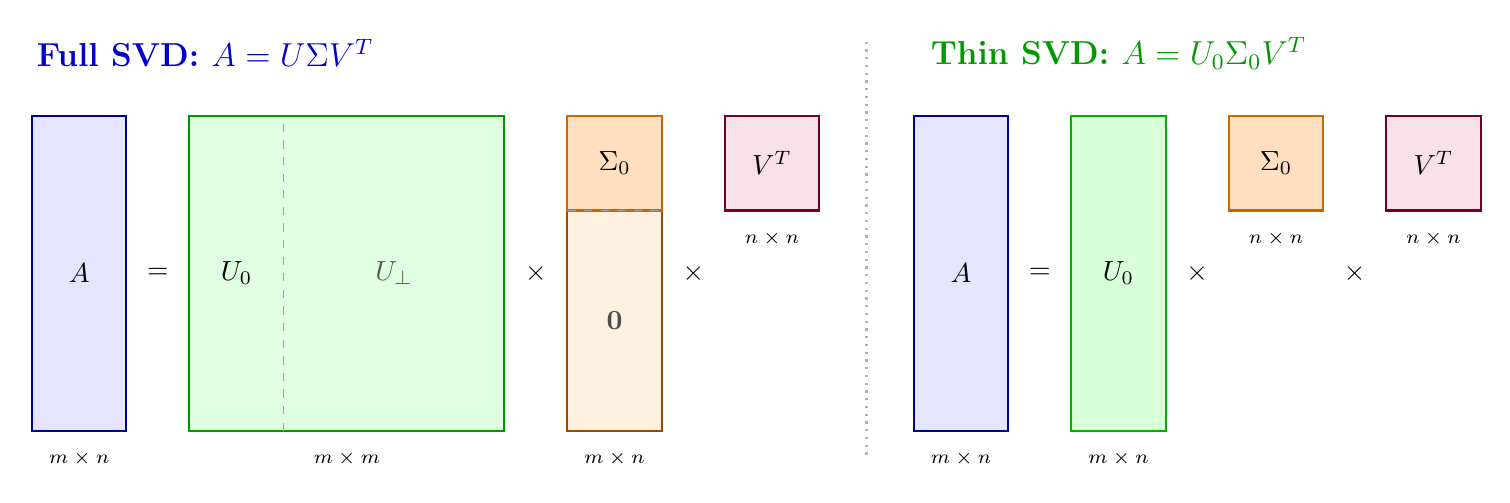
\begin{tikzpicture}[>=Stealth,
    brace/.style={decorate, decoration={brace, amplitude=5pt, raise=3pt}}]

    % --- FULL SVD ---
    \node[font=\bfseries\large, text=blue!80!black] at (2.2, 4.8) {Full SVD: $A = U \Sigma V^T$};

    % Matrix A (m x n)
    \draw[thick, fill=blue!10, draw=blue!60!black] (0, 0) rectangle (1.2, 4.0);
    \node at (0.6, 2.0) {$A$};
    \node[below=4pt, font=\scriptsize] at (0.6, 0) {$m \times n$};

    \node at (1.6, 2.0) {$=$};

    % Matrix U (m x m)
    \draw[thick, fill=green!12, draw=green!60!black] (2.0, 0) rectangle (6.0, 4.0);
    \draw[dashed, draw=gray!70] (3.2, 0) -- (3.2, 4.0);
    \node at (2.6, 2.0) {$U_0$};
    \node[text=gray!70!black] at (4.6, 2.0) {$U_{\perp}$};
    \node[below=4pt, font=\scriptsize] at (4.0, 0) {$m \times m$};

    \node at (6.4, 2.0) {$\times$};

    % Matrix Sigma (m x n)
    \draw[thick, fill=orange!12, draw=orange!60!black] (6.8, 0) rectangle (8.0, 4.0);
    \draw[thick, fill=orange!25, draw=orange!80!black] (6.8, 2.8) rectangle (8.0, 4.0);
    \draw[dashed, draw=gray!70] (6.8, 2.8) -- (8.0, 2.8);
    \node at (7.4, 3.4) {$\Sigma_0$};
    \node[text=gray!60!black] at (7.4, 1.4) {$\mathbf{0}$};
    \node[below=4pt, font=\scriptsize] at (7.4, 0) {$m \times n$};

    \node at (8.4, 2.0) {$\times$};

    % Matrix V^T (n x n)
    \draw[thick, fill=purple!12, draw=purple!60!black] (8.8, 2.8) rectangle (10.0, 4.0);
    \node at (9.4, 3.4) {$V^T$};
    \node[below=4pt, font=\scriptsize] at (9.4, 2.8) {$n \times n$};

    % --- DIVIDER ---
    \draw[dotted, thick, gray!60] (10.6, -0.3) -- (10.6, 5.0);

    % --- THIN SVD ---
    \node[font=\bfseries\large, text=green!60!black] at (13.8, 4.8) {Thin SVD: $A = U_0 \Sigma_0 V^T$};

    % Matrix A (m x n)
    \draw[thick, fill=blue!10, draw=blue!60!black] (11.2, 0) rectangle (12.4, 4.0);
    \node at (11.8, 2.0) {$A$};
    \node[below=4pt, font=\scriptsize] at (11.8, 0) {$m \times n$};

    \node at (12.8, 2.0) {$=$};

    % Matrix U_0 (m x n)
    \draw[thick, fill=green!15, draw=green!70!black] (13.2, 0) rectangle (14.4, 4.0);
    \node at (13.8, 2.0) {$U_0$};
    \node[below=4pt, font=\scriptsize] at (13.8, 0) {$m \times n$};

    \node at (14.8, 2.0) {$\times$};

    % Matrix Sigma_0 (n x n)
    \draw[thick, fill=orange!25, draw=orange!80!black] (15.2, 2.8) rectangle (16.4, 4.0);
    \node at (15.8, 3.4) {$\Sigma_0$};
    \node[below=4pt, font=\scriptsize] at (15.8, 2.8) {$n \times n$};

    \node at (16.8, 2.0) {$\times$};

    % Matrix V^T (n x n)
    \draw[thick, fill=purple!12, draw=purple!60!black] (17.2, 2.8) rectangle (18.4, 4.0);
    \node at (17.8, 3.4) {$V^T$};
    \node[below=4pt, font=\scriptsize] at (17.8, 2.8) {$n \times n$};

\end{tikzpicture}
}
\caption{Structural and dimensional comparison between Full SVD and Economy (Thin) SVD for tall matrices ($m \ge n$). Thin SVD eliminates the zero rows of $\Sigma$ and the unneeded trailing columns $U_{\perp}$.}
\label{fig:full-vs-thin-svd-structure-en}
\end{figure}

\subsection{Computational Efficiency and Subspace Semantics}

\begin{itemize}
    \item \textbf{Memory Storage:} Storing full $U \in \R^{m \times m}$ requires $\BigO{m^2}$ elements. When $m = 10^5$ and $n = 10^2$, storing $U$ consumes approximately $80$ Gigabytes of RAM in double precision. In contrast, storing $U_0 \in \R^{m \times n}$ requires only $m \cdot n = 10^7$ floats ($\approx 80$ Megabytes).
    \item \textbf{Floating-Point Flops:} Full SVD requires computing all $m$ orthogonal directions in $\R^m$ ($\BigO{m^2 n}$ or $\BigO{m^3}$ operations), whereas Thin SVD executes in $\BigO{m n^2}$ flops.
    \item \textbf{Subspace Relations:}
    \begin{equation}
        \operatorname{Im}(A) = \spanop\{\mathbf{u}_1, \dots, \mathbf{u}_r\} \subseteq \spanop(U_0), \qquad \ker(A^T) = \spanop(U_{\perp}).
    \end{equation}
    Thin SVD retains the complete geometry of the range of $A$. The orthogonal complement $U_{\perp}$ spans the null space of $A^T$ and can be omitted in most practical applications.
\end{itemize}

\FloatBarrier
\section{Matrix Norms and Induced Norms}
\label{sec:matrix-norms-induced-en}

Just as vector norms measure the magnitude or length of vectors in $\R^n$, matrix norms provide a rigorous metric to quantify the magnitude of linear operators or measure approximation errors.

\subsection{Axiomatic Definition of Matrix Norms}

\begin{definition}[General Matrix Norm]
A function $\|\cdot\|: \R^{m \times n} \to \R$ is called a \textbf{matrix norm} if it satisfies the following four fundamental axioms for all matrices $A, B \in \R^{m \times n}$ and every scalar $\alpha \in \R$:
\begin{enumerate}
    \item \textbf{Non-negativity and definiteness:}
    \begin{equation}
        \|A\| \ge 0, \quad \text{and} \quad \|A\| = 0 \iff A = \mathbf{0}_{m \times n}.
    \end{equation}
    \item \textbf{Absolute homogeneity:}
    \begin{equation}
        \|\alpha A\| = |\alpha| \cdot \|A\|.
    \end{equation}
    \item \textbf{Triangle inequality:}
    \begin{equation}
        \|A + B\| \le \|A\| + \|B\|.
    \end{equation}
    \item \textbf{Sub-multiplicativity:} For matrices of compatible dimensions ($A \in \R^{m \times n}, B \in \R^{n \times p}$),
    \begin{equation}
        \|AB\| \le \|A\| \cdot \|B\|.
    \end{equation}
\end{enumerate}
\end{definition}

\subsection{Matrix Norms Induced by Vector Norms}

Given a vector norm $\|\cdot\|$ defined on both domain $\R^n$ and codomain $\R^m$, the canonical \textbf{induced matrix norm} (or \textit{operator norm}) is defined as follows:

\begin{definition}[Induced Matrix Norm]
The matrix norm induced by a vector norm $\|\cdot\|$ measures the maximum factor by which $A$ can stretch any non-zero vector:
\begin{equation}
    \|A\| := \max_{\mathbf{v} \in \R^n, \mathbf{v} \neq \mathbf{0}} \frac{\|A\mathbf{v}\|}{\|\mathbf{v}\|}.
\end{equation}
By homogeneity, setting $\mathbf{x} = \mathbf{v} / \|\mathbf{v}\|$ (so that $\|\mathbf{x}\| = 1$), the definition is equivalent to optimization over the unit sphere:
\begin{equation}
    \label{eq:def-induced-norm-sphere-en}
    \|A\| = \max_{\|\mathbf{x}\| = 1} \|A\mathbf{x}\|.
\end{equation}
\end{definition}

\begin{noteblock}{Notational Convention}
The same double-bar symbol $\|\cdot\|$ denotes both vector norms and matrix norms. Context resolves any ambiguity: in $\|A\mathbf{x}\|$, the argument is a vector in $\R^m$, whereas in $\|A\|$, the argument is the matrix $A \in \R^{m \times n}$.
\end{noteblock}

From~\eqref{eq:def-induced-norm-sphere-en}, the fundamental compatibility inequality follows directly:
\begin{equation}
    \|A\mathbf{v}\| \le \|A\| \cdot \|\mathbf{v}\| \quad \forall \mathbf{v} \in \R^n.
\end{equation}

\FloatBarrier
\section{The Spectral Norm (Matrix 2-Norm)}
\label{sec:spectral-norm-en}

The \textbf{spectral norm} (matrix 2-norm), denoted by $\|A\|_2$, is the matrix norm induced by the standard Euclidean vector norm ($\ell_2$ norm):
\begin{equation}
    \|\mathbf{x}\|_2 = \sqrt{\mathbf{x}^T \mathbf{x}} = \sqrt{\sum_{i=1}^n x_i^2}.
\end{equation}
Thus:
\begin{equation}
    \|A\|_2 := \max_{\mathbf{x} \neq \mathbf{0}} \frac{\|A\mathbf{x}\|_2}{\|\mathbf{x}\|_2} = \max_{\|\mathbf{x}\|_2 = 1} \|A\mathbf{x}\|_2.
\end{equation}

\subsection{Step-by-Step Derivation via SVD}

\begin{theorem}[Characterization of the Spectral Norm]
\label{thm:spectral-norm-sigma1-en}
For any real matrix $A \in \R^{m \times n}$, its spectral norm $\|A\|_2$ equals its largest singular value:
\begin{equation}
    \|A\|_2 = \sigma_1.
\end{equation}
\end{theorem}

\begin{proof}
We carry out the proof in four sequential steps:

\paragraph{Step 1: Substituting the Full SVD.}
Substitute $A = U \Sigma V^T$ into the definition:
\begin{equation}
    \|A\|_2 = \max_{\mathbf{x} \neq \mathbf{0}} \frac{\|U \Sigma V^T \mathbf{x}\|_2}{\|\mathbf{x}\|_2}.
\end{equation}

\paragraph{Step 2: Isometric invariance of orthogonal $U$.}
Because $U \in \R^{m \times m}$ is orthogonal, by the Euclidean isometry theorem proved in Chapter~\ref{chap:matrix-multiplication-complexity-orthogonality} (Theorem~\ref{thm:en:orthogonal-isometry}, page~\pageref{thm:en:orthogonal-isometry}), it preserves Euclidean vector lengths:
\begin{equation}
    \|U \mathbf{y}\|_2 = \|\mathbf{y}\|_2 \quad \forall \mathbf{y} \in \R^m.
\end{equation}
Setting $\mathbf{y} = \Sigma V^T \mathbf{x} \in \R^m$, the factor $U$ can be eliminated:
\begin{equation}
    \|U \Sigma V^T \mathbf{x}\|_2 = \|\Sigma V^T \mathbf{x}\|_2 \implies \|A\|_2 = \max_{\mathbf{x} \neq \mathbf{0}} \frac{\|\Sigma V^T \mathbf{x}\|_2}{\|\mathbf{x}\|_2}.
\end{equation}

\paragraph{Step 3: Change of variables via orthogonal $V$.}
Define $\mathbf{z} := V^T \mathbf{x} \in \R^n$. Again by the isometry property of orthogonal matrices (Theorem~\ref{thm:en:orthogonal-isometry}), $\|\mathbf{x}\|_2 = \|V \mathbf{z}\|_2 = \|\mathbf{z}\|_2$. Because $V^T$ establishes an isometric linear bijection on $\R^n$, the maximization maps directly to $\mathbf{z}$:
\begin{equation}
    \|A\|_2 = \max_{\mathbf{z} \neq \mathbf{0}} \frac{\|\Sigma \mathbf{z}\|_2}{\|\mathbf{z}\|_2} = \max_{\|\mathbf{z}\|_2 = 1} \|\Sigma \mathbf{z}\|_2.
\end{equation}

\paragraph{Step 4: Explicit optimization on the unit sphere.}
Evaluating $\Sigma \mathbf{z}$ componentwise:
\begin{equation}
    \Sigma \mathbf{z} = \begin{bmatrix} \sigma_1 z_1 \\ \sigma_2 z_2 \\ \vdots \\ \sigma_r z_r \\ 0 \\ \vdots \end{bmatrix} \implies \|\Sigma \mathbf{z}\|_2^2 = \sum_{i=1}^r \sigma_i^2 z_i^2.
\end{equation}
Subject to $\sum_{i=1}^n z_i^2 = 1$, the convex combination of non-negative weights $w_i = z_i^2$ is maximized by placing the entire unit mass on the largest coefficient $\sigma_1^2$:
\begin{equation}
    \sum_{i=1}^r \sigma_i^2 z_i^2 \le \sigma_1^2 \sum_{i=1}^r z_i^2 \le \sigma_1^2 (1) = \sigma_1^2.
\end{equation}
This bound is attained by $\mathbf{z} = \mathbf{e}_1 = [1, 0, \dots, 0]^T$ (which corresponds to $\mathbf{x} = \mathbf{v}_1$). Taking square roots yields:
\begin{equation}
    \|A\|_2 = \sigma_1.
\end{equation}
\end{proof}

\begin{corollary}[Unitary Invariance of the Spectral Norm]
The spectral norm is unchanged by left or right orthogonal multiplications:
\begin{equation}
    \|Q_1 A Q_2\|_2 = \|A\|_2 \quad \forall Q_1 \in \R^{m \times m}, Q_2 \in \R^{n \times n} \text{ orthogonal}.
\end{equation}
\end{corollary}

\FloatBarrier
\section{The Frobenius Norm}
\label{sec:frobenius-norm-en}

The \textbf{Frobenius norm} is not an induced operator norm; rather, it extends Euclidean vector distance by treating $A \in \R^{m \times n}$ as an unwrapped vector in $\R^{m \cdot n}$.

\subsection{Definition and Trace Formulation}

\begin{definition}[Frobenius Norm]
The Frobenius norm $\|A\|_F$ of $A \in \R^{m \times n}$ is defined by:
\begin{equation}
    \|A\|_F := \sqrt{\sum_{i=1}^m \sum_{j=1}^n a_{ij}^2}.
\end{equation}
\end{definition}

This norm can be concisely expressed using the matrix \textbf{trace} $\trace(M) = \sum_i M_{ii}$:

\begin{proposition}[Trace Formulation]
\begin{equation}
    \|A\|_F = \sqrt{\trace(A^T A)} = \sqrt{\trace(A A^T)}.
\end{equation}
\end{proposition}

\begin{proof}
The $j$-th diagonal entry of $A^T A \in \R^{n \times n}$ is the squared Euclidean norm of the $j$-th column of $A$:
\begin{equation}
    (A^T A)_{jj} = \sum_{k=1}^m (A^T)_{jk} A_{kj} = \sum_{k=1}^m A_{kj}^2.
\end{equation}
Summing over all columns $j = 1, \dots, n$:
\begin{equation}
    \trace(A^T A) = \sum_{j=1}^n (A^T A)_{jj} = \sum_{j=1}^n \sum_{k=1}^m A_{kj}^2 = \sum_{i=1}^m \sum_{j=1}^n a_{ij}^2 = \|A\|_F^2.
\end{equation}
\end{proof}

\subsection{Spectral Representation via Singular Values}

\begin{theorem}[Frobenius Norm in Terms of Singular Values]
\label{thm:frobenius-singular-values-en}
The Frobenius norm of $A \in \R^{m \times n}$ equals the square root of the sum of squared singular values:
\begin{equation}
    \|A\|_F = \sqrt{\sum_{i=1}^r \sigma_i^2} = \sqrt{\sigma_1^2 + \sigma_2^2 + \dots + \sigma_r^2}.
\end{equation}
\end{theorem}

\begin{proof}
We exploit the cyclic property of the trace ($\trace(M_1 M_2 M_3) = \trace(M_2 M_3 M_1) = \trace(M_3 M_1 M_2)$):
\begin{enumerate}
    \item Substitute the SVD $A = U \Sigma V^T$:
    \begin{equation}
        \|A\|_F^2 = \trace(A^T A) = \trace\left( V \Sigma^T U^T U \Sigma V^T \right).
    \end{equation}
    \item Since $U$ is orthogonal, $U^T U = I_m$, leaving:
    \begin{equation}
        \|A\|_F^2 = \trace\left( V \Sigma^T \Sigma V^T \right).
    \end{equation}
    \item Permute $V$ cyclically to the end of the product:
    \begin{equation}
        \trace\left( V (\Sigma^T \Sigma V^T) \right) = \trace\left( \Sigma^T \Sigma (V^T V) \right).
    \end{equation}
    \item Since $V^T V = I_n$:
    \begin{equation}
        \|A\|_F^2 = \trace(\Sigma^T \Sigma) = \sum_{i=1}^r \sigma_i^2 \implies \|A\|_F = \sqrt{\sum_{i=1}^r \sigma_i^2}.
    \end{equation}
\end{enumerate}
\end{proof}

\begin{corollary}[Unitary Invariance of Frobenius Norm]
The Frobenius norm is also unitarily invariant:
\begin{equation}
    \|Q_1 A Q_2\|_F = \|A\|_F \quad \forall Q_1 \in \R^{m \times m}, Q_2 \in \R^{n \times n} \text{ orthogonal}.
\end{equation}
\end{corollary}

\FloatBarrier
\section{Complex Generalization and Symmetric Real Matrices}
\label{sec:complex-symmetric-matrices-en}

\subsection{Extension to Complex Vector Spaces ($\C$)}

\begin{itemize}
    \item \textbf{Conjugate Transpose (Adjoint):} The matrix adjoint $A^* \in \C^{n \times m}$ replaces the transpose:
    \begin{equation}
        (A^*)_{ij} = \overline{a_{ji}}.
    \end{equation}
    \item \textbf{Unitary Matrices:} A square complex matrix $Q \in \C^{n \times n}$ is \textbf{unitary} if:
    \begin{equation}
        Q^* Q = Q Q^* = I_n.
    \end{equation}
    \item \textbf{Hermitian Matrices:} A matrix $A \in \C^{n \times n}$ is \textbf{Hermitian} if $A^* = A$. Hermitian matrices have real eigenvalues and unitary eigenvectors.
    \item \textbf{Complex SVD:} For any $A \in \C^{m \times n}$:
    \begin{equation}
        A = U \Sigma V^*,
    \end{equation}
    where $U \in \C^{m \times m}$ and $V \in \C^{n \times n}$ are unitary, and $\Sigma \in \R^{m \times n}$ remains a \textbf{real} non-negative diagonal matrix ($\sigma_i \ge 0$).
\end{itemize}

\subsection{Deriving SVD from Spectral Decomposition for Symmetric Matrices}
\label{sec:svd-symmetric-recap-en}

As derived in detail in Problem~\ref{sec:en:svd-symmetric-spectral} of Chapter~\ref{chap:singular-value-decomposition-svd} (page~\pageref{sec:en:svd-symmetric-spectral}), for a real symmetric matrix ($A = A^T$) with known spectral decomposition $A = Q D Q^T = \sum_{i=1}^n d_i \mathbf{q}_i \mathbf{q}_i^T$, one does not need to form the Gram matrix $A^T A = A^2$. The SVD factors $A = U \Sigma V^T$ follow directly:
\begin{enumerate}
    \item \textbf{Singular values:} $\sigma_i = \sqrt{\lambda_i(A^T A)} = \sqrt{d_i^2} = |d_i| \ge 0$.
    \item \textbf{Right singular vectors:} $\mathbf{v}_i = \mathbf{q}_i$.
    \item \textbf{Left singular vectors:} $\mathbf{u}_i = \operatorname{sgn}(d_i) \mathbf{q}_i$, absorbing negative eigenvalue signs to maintain $d_i \mathbf{q}_i \mathbf{q}_i^T = |d_i| \mathbf{u}_i \mathbf{q}_i^T$.
    \item \textbf{Sorting:} Permute columns simultaneously to ensure non-increasing singular values $\sigma_1 \ge \sigma_2 \ge \dots \ge \sigma_n \ge 0$.
\end{enumerate}
This direct algebraic alignment links the spectral decomposition of symmetric operators to the general SVD, serving as the real counterpart to the complex unitary SVD developed above.

\FloatBarrier
\section{Low-Rank Matrix Approximation and the Eckart-Young Theorem}
\label{sec:eckart-young-en}

\subsection{Problem Formulation}

Given a target rank $k < \rank(A)$, we seek a rank-$k$ matrix $B \in \R^{m \times n}$ closest to $A$:
\begin{equation}
    \min_{B \in \R^{m \times n}, \, \rank(B) \le k} \|A - B\|.
\end{equation}

\subsection{Toy $2 \times 2$ Motivation}

Consider the rank-2 matrix analyzed in class:
\begin{equation}
    A = \begin{bmatrix} 1 & 2 \\ 3 & 4 \end{bmatrix}, \qquad \rank(A) = 2.
\end{equation}
\begin{itemize}
    \item \textbf{Attempt 1 (Row copy):} $B_1 = \begin{bmatrix} 1 & 2 \\ 2 & 4 \end{bmatrix} \implies \|A - B_1\|_F = 1.0$.
    \item \textbf{Attempt 2 (Single-entry balance):} $B_2 = \begin{bmatrix} 1.5 & 2 \\ 3 & 4 \end{bmatrix} \implies \|A - B_2\|_F = 0.5$.
    \item \textbf{Optimal SVD Solution:} The singular values of $A$ are $\sigma_1 \approx 5.465, \sigma_2 \approx 0.366$. The theoretical minimum achievable error is $\sigma_2 \approx 0.366 < 0.5$.
\end{itemize}

\subsection{The Eckart-Young-Mirsky Theorem}

\begin{theorem}[Eckart-Young-Mirsky]
\label{thm:eckart-young-en}
Let $A \in \R^{m \times n}$ with SVD $A = \sum_{i=1}^r \sigma_i \mathbf{u}_i \mathbf{v}_i^T$. For any $k < r$, the truncated SVD matrix:
\begin{equation}
    A_k := \sum_{i=1}^k \sigma_i \mathbf{u}_i \mathbf{v}_i^T = U_k \Sigma_k V_k^T
\end{equation}
is the global minimizer of $\min_{\rank(B) \le k} \|A - B\|$ under both the spectral norm $\|\cdot\|_2$ and the Frobenius norm $\|\cdot\|_F$ (and any unitarily invariant norm).
\end{theorem}

\subsection{Exact Residual Error Formulas}

The residual matrix is $A - A_k = \sum_{i=k+1}^r \sigma_i \mathbf{u}_i \mathbf{v}_i^T$. By Theorems~\ref{thm:spectral-norm-sigma1-en} and~\ref{thm:frobenius-singular-values-en}:

\begin{alertblock}{Exact SVD Truncation Errors}
\begin{enumerate}
    \item \textbf{Spectral Norm Error:}
    \begin{equation}
        \|A - A_k\|_2 = \sigma_{k+1}.
    \end{equation}
    \item \textbf{Frobenius Norm Error:}
    \begin{equation}
        \|A - A_k\|_F = \sqrt{\sum_{i=k+1}^r \sigma_i^2} = \sqrt{\sigma_{k+1}^2 + \dots + \sigma_r^2}.
    \end{equation}
\end{enumerate}
\end{alertblock}

\begin{figure}[H]
\centering
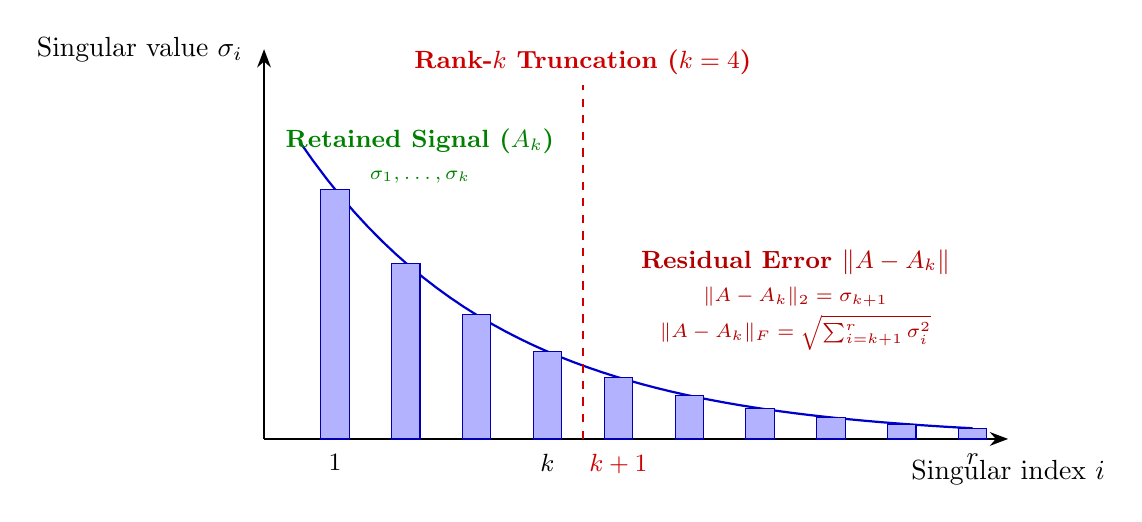
\begin{tikzpicture}[>=Stealth, scale=0.9]
    \draw[->, thick] (0, 0) -- (10.5, 0) node[below=4pt] {Singular index $i$};
    \draw[->, thick] (0, 0) -- (0, 5.5) node[left=4pt] {Singular value $\sigma_i$};

    \draw[thick, blue!80!black, domain=0.5:10, samples=50] plot (\x, {5 * exp(-0.35 * \x)});

    \foreach \x/\y in {1/3.52, 2/2.48, 3/1.75, 4/1.23, 5/0.87, 6/0.61, 7/0.43, 8/0.30, 9/0.21, 10/0.15} {
        \draw[fill=blue!30, draw=blue!70!black] (\x - 0.2, 0) rectangle (\x + 0.2, \y);
    }

    \draw[thick, dashed, red!80!black] (4.5, 0) -- (4.5, 5.0) node[above, font=\small\bfseries] {Rank-$k$ Truncation ($k=4$)};

    \node[text=green!50!black, font=\small\bfseries] at (2.2, 4.2) {Retained Signal ($A_k$)};
    \node[text=green!50!black, font=\scriptsize] at (2.2, 3.7) {$\sigma_1, \dots, \sigma_k$};

    \node[text=red!70!black, font=\small\bfseries] at (7.5, 2.5) {Residual Error $\|A - A_k\|$};
    \node[text=red!70!black, font=\scriptsize] at (7.5, 2.0) {$\|A - A_k\|_2 = \sigma_{k+1}$};
    \node[text=red!70!black, font=\scriptsize] at (7.5, 1.5) {$\|A - A_k\|_F = \sqrt{\sum_{i=k+1}^r \sigma_i^2}$};

    \node[below=2pt, font=\small] at (1, 0) {$1$};
    \node[below=2pt, font=\small] at (4, 0) {$k$};
    \node[below=2pt, font=\small, text=red!80!black] at (5, 0) {$k+1$};
    \node[below=2pt, font=\small] at (10, 0) {$r$};
\end{tikzpicture}
\caption{Singular spectrum decay and energy partitioning between retained signal ($A_k$) and discarded residual error quantified by the Eckart-Young Theorem.}
\label{fig:eckart-young-spectrum-en}
\end{figure}

\FloatBarrier
\section{Geometric Interpretation: From Sphere to Ellipsoid}
\label{sec:geometric-interpretation-en}

The SVD factors any linear mapping into three sequential geometric steps:

\begin{figure}[H]
\centering
\resizebox{0.95\textwidth}{!}{%
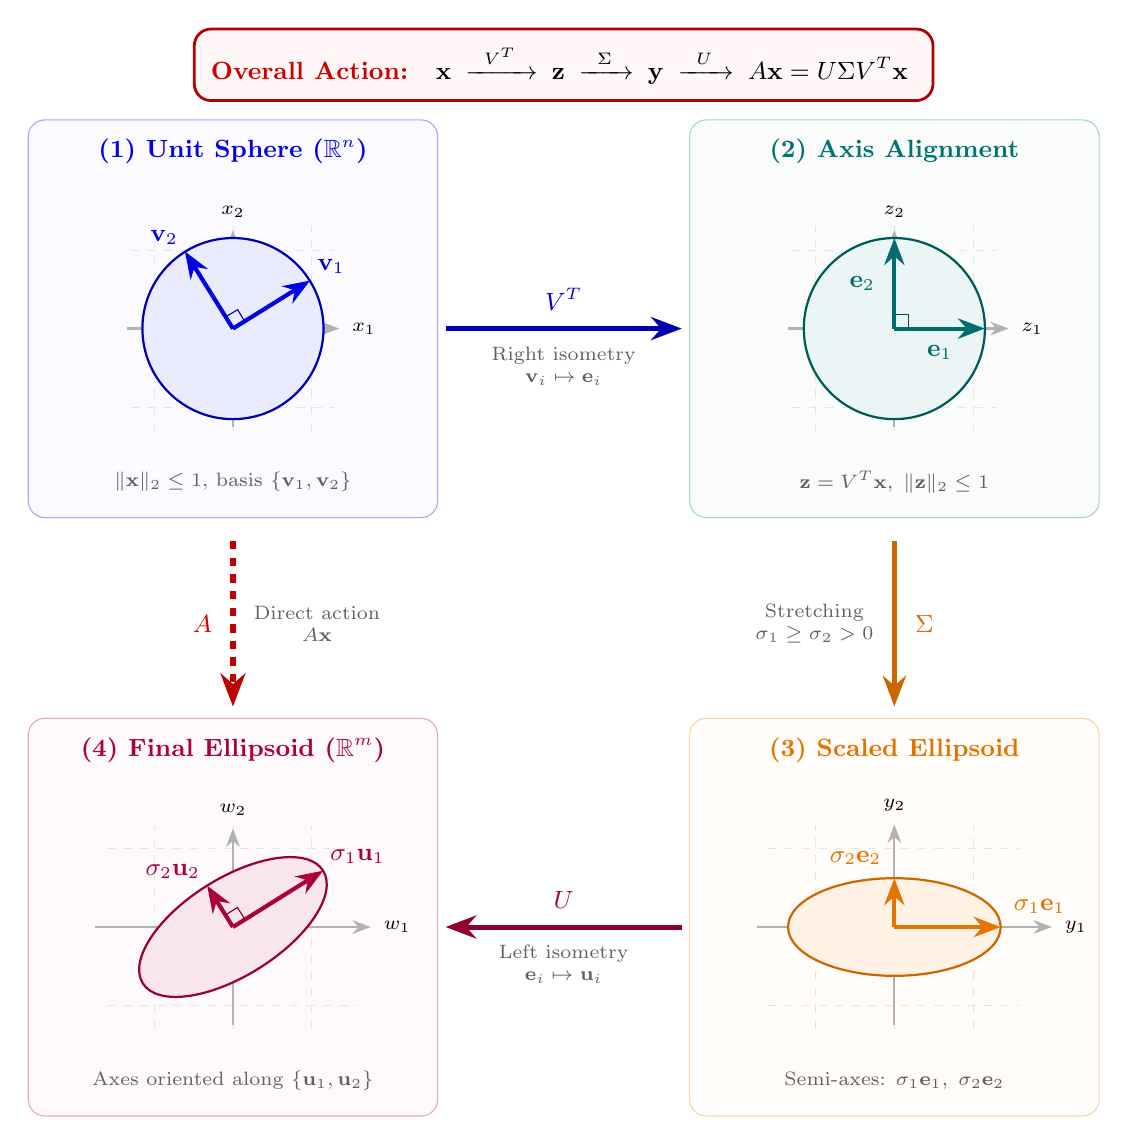
\begin{tikzpicture}[>=Stealth, scale=1.0]

    % =========================================================================
    % TOP BANNER: SVD Decomposition and Global Matrix Action
    % =========================================================================
    \node[draw=red!70!black, fill=red!3, rounded corners=6pt, inner sep=6pt, align=center, line width=1pt] at (0, 7.15) {
        \textbf{\textcolor{red!80!black}{\small Overall Action:}}\quad
        \small $\mathbf{x} \;\xrightarrow{\;\; V^T \;\;}\; \mathbf{z} \;\xrightarrow{\;\; \Sigma \;\;}\; \mathbf{y} \;\xrightarrow{\;\; U \;\;}\; A\mathbf{x} = U \Sigma V^T \mathbf{x}$
    };

    % =========================================================================
    % QUADRANT 1 (Top-Left): Original Unit Sphere in R^n
    % =========================================================================
    \begin{scope}[shift={(-4.2, 3.8)}]
        \draw[draw=blue!35, fill=blue!2, rounded corners=6pt] (-2.6, -2.4) rectangle (2.6, 2.65);
        \node[font=\small\bfseries, text=blue!90!black, align=center] at (0, 2.25) {(1) Unit Sphere ($\R^n$)};

        \draw[help lines, color=gray!20, dashed] (-1.3,-1.3) grid (1.3,1.3);
        \draw[->, thick, gray!60] (-1.35, 0) -- (1.35, 0) node[right=1pt, font=\scriptsize, text=black] {$x_1$};
        \draw[->, thick, gray!60] (0, -1.25) -- (0, 1.25) node[above=1pt, font=\scriptsize, text=black] {$x_2$};

        % Unit sphere
        \draw[thick, fill=blue!8, draw=blue!70!black] (0, 0) circle (1.15);

        % Orthonormal right singular vectors v_1 and v_2
        \draw[->, line width=1.5pt, blue!90!black] (0, 0) -- (0.98, 0.61) node[above right=-2pt, font=\small\bfseries] {$\mathbf{v}_1$};
        \draw[->, line width=1.5pt, blue!90!black] (0, 0) -- (-0.61, 0.98) node[above left=-2pt, font=\small\bfseries] {$\mathbf{v}_2$};

        % Right-angle mark
        \draw[thin, blue!60!black] (0.15, 0.09) -- (0.06, 0.24) -- (-0.09, 0.15);

        \node[font=\scriptsize, text=gray!75!black, align=center] at (0, -1.95) {$\|\mathbf{x}\|_2 \le 1$, basis $\{\mathbf{v}_1, \mathbf{v}_2\}$};
    \end{scope}

    % --- TRANSITION 1 -> 2: Right Isometry V^T ---
    \draw[->, line width=1.8pt, blue!70!black] (-1.5, 3.8) -- (1.5, 3.8);
    \node[above=3pt, font=\small\bfseries, text=blue!85!black] at (0, 3.8) {$V^T$};
    \node[below=3pt, font=\scriptsize, align=center, text=gray!75!black] at (0, 3.8) {Right isometry\\$\mathbf{v}_i \mapsto \mathbf{e}_i$};

    % =========================================================================
    % QUADRANT 2 (Top-Right): Axis-Aligned Sphere
    % =========================================================================
    \begin{scope}[shift={(4.2, 3.8)}]
        \draw[draw=teal!35, fill=teal!2, rounded corners=6pt] (-2.6, -2.4) rectangle (2.6, 2.65);
        \node[font=\small\bfseries, text=teal!90!black, align=center] at (0, 2.25) {(2) Axis Alignment};

        \draw[help lines, color=gray!20, dashed] (-1.3,-1.3) grid (1.3,1.3);
        \draw[->, thick, gray!60] (-1.35, 0) -- (1.45, 0) node[right=1pt, font=\scriptsize, text=black] {$z_1$};
        \draw[->, thick, gray!60] (0, -1.25) -- (0, 1.25) node[above=1pt, font=\scriptsize, text=black] {$z_2$};

        % Transformed unit sphere
        \draw[thick, fill=teal!8, draw=teal!70!black] (0, 0) circle (1.15);

        % Canonical standard basis vectors
        \draw[->, line width=1.5pt, teal!85!black] (0, 0) -- (1.15, 0) node[midway, below=2pt, font=\small\bfseries] {$\mathbf{e}_1$};
        \draw[->, line width=1.5pt, teal!85!black] (0, 0) -- (0, 1.15) node[midway, left=3pt, font=\small\bfseries] {$\mathbf{e}_2$};

        % Right-angle mark
        \draw[thin, teal!60!black] (0.18, 0) -- (0.18, 0.18) -- (0, 0.18);

        \node[font=\scriptsize, text=gray!75!black, align=center] at (0, -1.95) {$\mathbf{z} = V^T \mathbf{x}, \; \|\mathbf{z}\|_2 \le 1$};
    \end{scope}

    % --- TRANSITION 2 -> 3: Diagonal Stretching Sigma ---
    \draw[->, line width=1.8pt, orange!80!black] (4.2, 1.1) -- (4.2, -1.0);
    \node[right=4pt, font=\small\bfseries, text=orange!85!black] at (4.2, 0.05) {$\Sigma$};
    \node[left=4pt, font=\scriptsize, align=center, text=gray!75!black] at (4.2, 0.05) {Stretching\\$\sigma_1 \ge \sigma_2 > 0$};

    % =========================================================================
    % QUADRANT 3 (Bottom-Right): Scaled Ellipsoid
    % =========================================================================
    \begin{scope}[shift={(4.2, -3.8)}]
        \draw[draw=orange!35, fill=orange!2, rounded corners=6pt] (-2.6, -2.4) rectangle (2.6, 2.65);
        \node[font=\small\bfseries, text=orange!90!black, align=center] at (0, 2.25) {(3) Scaled Ellipsoid};

        \draw[help lines, color=gray!20, dashed] (-1.6,-1.3) grid (1.6,1.3);
        \draw[->, thick, gray!60] (-1.75, 0) -- (2.0, 0) node[right=1pt, font=\scriptsize, text=black] {$y_1$};
        \draw[->, thick, gray!60] (0, -1.25) -- (0, 1.3) node[above=1pt, font=\scriptsize, text=black] {$y_2$};

        % Ellipsoid
        \draw[thick, fill=orange!10, draw=orange!80!black] (0, 0) ellipse (1.35 and 0.62);

        % Semi-axes
        \draw[->, line width=1.5pt, orange!90!black] (0, 0) -- (1.35, 0) node[above right=1pt, font=\small\bfseries] {$\sigma_1 \mathbf{e}_1$};
        \draw[->, line width=1.5pt, orange!90!black] (0, 0) -- (0, 0.62) node[above left=1pt, font=\small\bfseries] {$\sigma_2 \mathbf{e}_2$};

        \node[font=\scriptsize, text=gray!75!black, align=center] at (0, -1.95) {Semi-axes: $\sigma_1 \mathbf{e}_1, \; \sigma_2 \mathbf{e}_2$};
    \end{scope}

    % --- TRANSITION 3 -> 4: Left Isometry U ---
    \draw[->, line width=1.8pt, purple!75!black] (1.5, -3.8) -- (-1.5, -3.8);
    \node[above=3pt, font=\small\bfseries, text=purple!85!black] at (0, -3.8) {$U$};
    \node[below=3pt, font=\scriptsize, align=center, text=gray!75!black] at (0, -3.8) {Left isometry\\$\mathbf{e}_i \mapsto \mathbf{u}_i$};

    % =========================================================================
    % QUADRANT 4 (Bottom-Left): Final Rotated Ellipsoid in R^m
    % =========================================================================
    \begin{scope}[shift={(-4.2, -3.8)}]
        \draw[draw=purple!35, fill=purple!2, rounded corners=6pt] (-2.6, -2.4) rectangle (2.6, 2.65);
        \node[font=\small\bfseries, text=purple!90!black, align=center] at (0, 2.25) {(4) Final Ellipsoid ($\R^m$)};

        \draw[help lines, color=gray!20, dashed] (-1.6,-1.3) grid (1.6,1.3);
        \draw[->, thick, gray!60] (-1.75, 0) -- (1.75, 0) node[right=1pt, font=\scriptsize, text=black] {$w_1$};
        \draw[->, thick, gray!60] (0, -1.25) -- (0, 1.25) node[above=1pt, font=\scriptsize, text=black] {$w_2$};

        % Ellipsoid rotated by 32 degrees
        \draw[thick, fill=purple!10, draw=purple!80!black, rotate=32] (0, 0) ellipse (1.35 and 0.62);

        % Rotated left singular vectors
        \draw[->, line width=1.5pt, purple!90!black] (0, 0) -- (1.145, 0.715) node[above right=-2pt, font=\small\bfseries] {$\sigma_1 \mathbf{u}_1$};
        \draw[->, line width=1.5pt, purple!90!black] (0, 0) -- (-0.328, 0.526) node[above left=-2pt, font=\small\bfseries] {$\sigma_2 \mathbf{u}_2$};

        % Rotated right-angle mark
        \draw[thin, purple!60!black, rotate=32] (0.18, 0) -- (0.18, 0.18) -- (0, 0.18);

        \node[font=\scriptsize, text=gray!75!black, align=center] at (0, -1.95) {Axes oriented along $\{\mathbf{u}_1, \mathbf{u}_2\}$};
    \end{scope}

    % --- TRANSITION 1 -> 4 DIRECT: Global action A (Diagram closure) ---
    \draw[->, line width=2pt, dashed, red!75!black] (-4.2, 1.1) -- (-4.2, -1.0);
    \node[left=4pt, font=\small\bfseries, text=red!85!black] at (-4.2, 0.05) {$A$};
    \node[right=4pt, font=\scriptsize, align=center, text=gray!75!black] at (-4.2, 0.05) {Direct action\\$A\mathbf{x}$};

\end{tikzpicture}%
}
\caption{Four-quadrant geometric interpretation of the linear mapping $A = U \Sigma V^T$ acting on the unit Euclidean sphere: (1) Initial unit sphere with orthonormal right singular basis $\mathbf{v}_i$; (2) Right isometry $V^T$ aligning $\mathbf{v}_i$ to the canonical axes; (3) Axis-aligned dilation $\Sigma$ producing an ellipsoid with semi-axes $\sigma_i$; (4) Final left isometry $U$ orienting principal axes along the left singular vectors $\mathbf{u}_i$.}
\label{fig:svd-geometric-transformation-en}
\end{figure}

\FloatBarrier
\section{Application 1: Image Compression via Truncated SVD}
\label{sec:application-image-compression-en}

\subsection{Matrix Representation of Grayscale Images}

A grayscale image of resolution $m \times n$ is represented by a matrix $A \in \R^{m \times n}$. Uncompressed storage requires $m \cdot n$ pixel values.

\subsection{Rank-$k$ Approximation and Compression Ratio}

Replacing $A$ with its truncated rank-$k$ approximation $A_k = U_k \Sigma_k V_k^T$, we only store:
\begin{equation}
    \text{Storage}(A_k) = k(m + n + 1) \text{ values}.
\end{equation}
The compression ratio is:
\begin{equation}
    \rho_k = \frac{k(m + n + 1)}{m \cdot n}.
\end{equation}

For an image of size $600 \times 402$ ($241\,200$ entries), $k = 10$ requires only $10\,030$ entries ($\approx 4.1\%$ of original storage), while $k = 30$ achieves high perceptual fidelity with only $12.5\%$ of the original data.

\FloatBarrier
\section{Application 2: Tabular Data and Anomaly Detection}
\label{sec:application-tabular-anomalies-en}

Consider the test grade matrix of $4$ students across $3$ tests:
\begin{equation}
    M = \begin{bmatrix}
        90 & 95 & 55 \\
        32 & 35 & 20 \\
        70 & 75 & 50 \\
        70 & 31 & 49
    \end{bmatrix} \approx \mathbf{x} \mathbf{y}^T = \begin{bmatrix} x_1 \\ x_2 \\ x_3 \\ x_4 \end{bmatrix} \begin{bmatrix} y_1 & y_2 & y_3 \end{bmatrix}.
\end{equation}

\begin{itemize}
    \item $\mathbf{y}^T = [y_1, y_2, y_3]$ measures relative test ease ($y_3$ is lower for harder test C).
    \item $\mathbf{x} = [x_1, x_2, x_3, x_4]^T$ measures student overall ability.
    \item In the residual matrix $R = M - \sigma_1 \mathbf{u}_1 \mathbf{v}_1^T$:
    \begin{itemize}
        \item $r_{ij} \gg 0$: Anomaly indicating unexpectedly high score (cheating or targeted preparation).
        \item $r_{ij} \ll 0$: Sudden performance drop (illness or technical issue, such as student 4 on test B).
    \end{itemize}
\end{itemize}

\FloatBarrier
\section{Application 3: Principal Component Analysis (PCA) via SVD}
\label{sec:application-pca-svd-en}

Given $n$ samples $\mathbf{x}_1, \dots, \mathbf{x}_n \in \R^m$, form $A = [\mathbf{x}_1, \dots, \mathbf{x}_n] \in \R^{m \times n}$.
\begin{enumerate}
    \item \textbf{Mean-centering:} Compute $\boldsymbol{\mu} = \frac{1}{n} \sum \mathbf{x}_i$ and centered data $\widehat{A} = A - \boldsymbol{\mu} \mathbf{1}_n^T$.
    \item \textbf{Sample Covariance:} $C = \frac{1}{n} \widehat{A}\widehat{A}^T \in \R^{m \times m}$.
    \item \textbf{SVD Connection:} Let $\widehat{A} = U \Sigma V^T$. Then:
    \begin{equation}
        C = \frac{1}{n} U \Sigma (V^T V) \Sigma^T U^T = U \left( \frac{1}{n} \Sigma \Sigma^T \right) U^T.
    \end{equation}
    The principal components are precisely the columns of $U$.
    \item The first principal component $\mathbf{u}_1$ points along maximal data variance ($\sigma_1^2 / n$).
\end{enumerate}

\begin{figure}[H]
\centering
\resizebox{0.95\textwidth}{!}{%
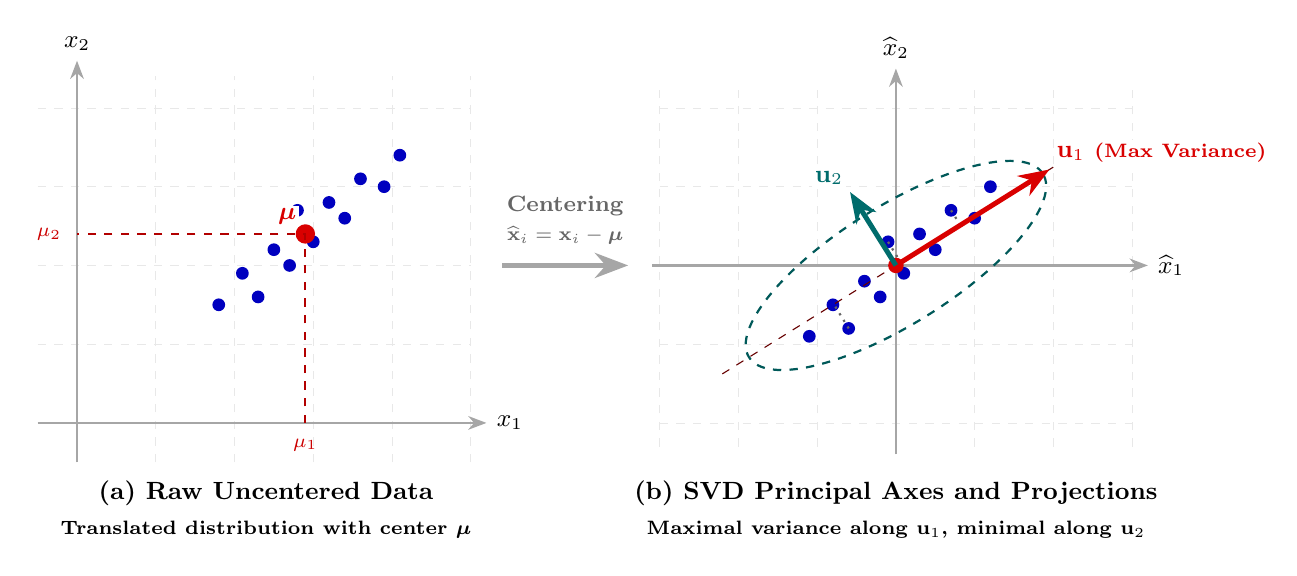
\begin{tikzpicture}[>=Stealth, scale=1.0]

    % =========================================================================
    % PANEL (a): Raw Uncentered Data
    % =========================================================================
    \begin{scope}[shift={(0, 0)}]
        \draw[help lines, color=gray!18, dashed] (-0.5,-0.5) grid (5.0,4.4);
        \draw[->, thick, gray!70] (-0.5, 0) -- (5.2, 0) node[right, font=\small, text=black] {$x_1$};
        \draw[->, thick, gray!70] (0, -0.5) -- (0, 4.6) node[above, font=\small, text=black] {$x_2$};

        % Data cloud
        \foreach \x/\y in {1.8/1.5, 2.1/1.9, 2.3/1.6, 2.5/2.2, 2.7/2.0, 2.8/2.7, 3.0/2.3, 3.2/2.8, 3.4/2.6, 3.6/3.1, 3.9/3.0, 4.1/3.4} {
            \fill[blue!75!black] (\x, \y) circle (2.3pt);
        }

        % Sample Mean / Centroid mu
        \fill[red!85!black] (2.9, 2.4) circle (3.5pt);
        \node[above left=1pt, font=\small\bfseries, text=red!85!black, fill=white, inner sep=1pt] at (2.85, 2.45) {$\boldsymbol{\mu}$};
        \draw[dashed, red!70!black, thick] (2.9, 0) node[below=2pt, font=\scriptsize, text=red!80!black] {$\mu_1$} -- (2.9, 2.4) -- (0, 2.4) node[left=2pt, font=\scriptsize, text=red!80!black] {$\mu_2$};

        \node[font=\bfseries\small, align=center] at (2.4, -1.1) {(a) Raw Uncentered Data\\[2pt]\scriptsize Translated distribution with center $\boldsymbol{\mu}$};
    \end{scope}

    % =========================================================================
    % CENTRAL ARROW: Centering
    % =========================================================================
    \draw[->, line width=2pt, gray!70] (5.4, 2.0) -- (7.0, 2.0);
    \node[above=4pt, font=\footnotesize\bfseries, align=center, text=gray!80!black] at (6.2, 2.0) {Centering\\[1pt]\scriptsize $\widehat{\mathbf{x}}_i = \mathbf{x}_i - \boldsymbol{\mu}$};

    % =========================================================================
    % PANEL (b): Centered Data with Principal Axes and Projections
    % =========================================================================
    \begin{scope}[shift={(10.4, 2.0)}]
        \draw[help lines, color=gray!18, dashed] (-3.0,-2.3) grid (3.0,2.3);
        \draw[->, thick, gray!70] (-3.1, 0) -- (3.2, 0) node[right, font=\small, text=black] {$\widehat{x}_1$};
        \draw[->, thick, gray!70] (0, -2.4) -- (0, 2.5) node[above, font=\small, text=black] {$\widehat{x}_2$};

        % Centered points
        \foreach \x/\y in {-1.1/-0.9, -0.8/-0.5, -0.6/-0.8, -0.4/-0.2, -0.2/-0.4, -0.1/0.3, 0.1/-0.1, 0.3/0.4, 0.5/0.2, 0.7/0.7, 1.0/0.6, 1.2/1.0} {
            \fill[blue!75!black] (\x, \y) circle (2.3pt);
        }

        % Covariance dispersion ellipse
        \draw[thick, dashed, teal!70!black, rotate=32] (0, 0) ellipse (2.2 and 0.75);

        % First principal axis u_1 (line of maximal variance)
        \draw[dashed, red!40!black, thin] ({-2.6*cos(32)}, {-2.6*sin(32)}) -- ({2.7*cos(32)}, {2.7*sin(32)});

        % Orthogonal drop projections onto u_1
        \draw[dotted, gray!80!black, thick] (-0.1, 0.3) -- (0.06, 0.04);
        \draw[dotted, gray!80!black, thick] (0.7, 0.7) -- (0.82, 0.51);
        \draw[dotted, gray!80!black, thick] (-0.6, -0.8) -- (-0.79, -0.49);

        % Centroid at origin
        \fill[red!85!black] (0, 0) circle (2.8pt);

        % First Principal Component u_1
        \draw[->, line width=1.8pt, red!85!black] (0, 0) -- ({2.3*cos(32)}, {2.3*sin(32)}) 
            node[above right=1pt, font=\small\bfseries, fill=white, inner sep=1pt] {$\mathbf{u}_1$ \scriptsize(Max Variance)};

        % Second Principal Component u_2
        \draw[->, line width=1.8pt, teal!85!black] (0, 0) -- ({-1.1*sin(32)}, {1.1*cos(32)}) 
            node[above left=1pt, font=\small\bfseries, fill=white, inner sep=1pt] {$\mathbf{u}_2$};

        % Subcaption (b) perfectly aligned on same vertical baseline as (a)
        \node[font=\bfseries\small, align=center] at (0, -3.1) {(b) SVD Principal Axes and Projections\\[2pt]\scriptsize Maximal variance along $\mathbf{u}_1$, minimal along $\mathbf{u}_2$};
    \end{scope}

\end{tikzpicture}%
}
\caption{Geometric interpretation of PCA via SVD: (a) Original raw data with center $\boldsymbol{\mu}$; (b) Centered data with principal directions $\mathbf{u}_1$ (maximal variance) and orthogonal $\mathbf{u}_2$ obtained from the SVD of $\widehat{A} = U \Sigma V^T$, displaying orthogonal projections onto the optimal low-rank subspace.}
\label{fig:pca-geometry-2d-en}
\end{figure}

\FloatBarrier
\section{Summary Table}
\label{sec:summary-table-en}

\begin{table}[H]
\centering
\small
\renewcommand{\arraystretch}{1.3}
\begin{tabularx}{\textwidth}{p{4.2cm} p{4.6cm} X}
\toprule
\textbf{Concept / Tool} & \textbf{Mathematical Formula} & \textbf{Computational Significance} \\
\midrule
\textbf{Full SVD} & $A = U \Sigma V^T, \; U \in \R^{m \times m}, \; V \in \R^{n \times n}$ & Complete bases for domain, codomain, 4 subspaces. \\
\textbf{Thin SVD} & $A = U_0 \Sigma_0 V^T, \; U_0 \in \R^{m \times n}, \; \Sigma_0 \in \R^{n \times n}$ & Reduces storage $\BigO{m^2} \to \BigO{mn}$, preserves $\operatorname{Im}(A)$. \\
\textbf{Induced Norm} & $\|A\| = \max_{\|\mathbf{x}\|=1} \|A\mathbf{x}\|$ & Maximum operator amplification factor. \\
\textbf{Spectral Norm} & $\|A\|_2 = \sigma_1$ & Largest singular value; unitarily invariant. \\
\textbf{Frobenius Norm} & $\|A\|_F = \sqrt{\trace(A^T A)} = \sqrt{\sum \sigma_i^2}$ & Matrix Euclidean length; unitarily invariant. \\
\textbf{Real Symmetric SVD} & $\sigma_i = |d_i|, \; \mathbf{u}_i = \operatorname{sgn}(d_i)\mathbf{q}_i, \; \mathbf{v}_i = \mathbf{q}_i$ & Deduced directly from $A = Q D Q^T$. \\
\textbf{Eckart-Young ($A_k$)} & $A_k = \sum_{i=1}^k \sigma_i \mathbf{u}_i \mathbf{v}_i^T$ & Global minimizer for $\min_{\rank(B)\le k} \|A-B\|$. \\
\textbf{Spectral Error} & $\|A - A_k\|_2 = \sigma_{k+1}$ & First discarded singular value. \\
\textbf{Frobenius Error} & $\|A - A_k\|_F = \sqrt{\sum_{i=k+1}^r \sigma_i^2}$ & Total discarded energy. \\
\textbf{Image Compression} & Storage $= k(m + n + 1) \ll mn$ & High-fidelity compression for decaying spectrum. \\
\textbf{PCA via SVD} & $\widehat{A} = U \Sigma V^T, \; C = \frac{1}{n} U \Sigma \Sigma^T U^T$ & Columns of $U$ are covariance eigenvectors. \\
\bottomrule
\end{tabularx}
\caption{Comprehensive overview of matrix norms, SVD factorizations, low-rank approximations, and applications.}
\label{tab:summary-svd-norms-en}
\end{table}

\chapter[QR Factorization and Householder Reflections]{QR Factorization and Householder Reflections:\\Geometry, Numerical Stability, and Algorithms}
\label{chap:qr-factorization-householder-reflections}
\label{chap:fattorizzazione-qr-riflessioni-householder-en}

This chapter introduces and constructively analyzes the \textbf{QR Factorization}, one of the cornerstones of modern numerical linear algebra for scientific computing, overdetermined linear systems (least squares problems), and spectral eigenvalue computation~\cite{golub2013matrix,trefethen1997numerical}. After formalizing the general existence theorem and the geometric distinction between the full decomposition (\textit{Full QR}) and the economical variant (\textit{Thin QR}), we introduce the family of \textbf{Householder reflectors} (elementary rank-1 orthogonal transformations). We prove the fundamental reflection lemma and address the critical impact of finite-precision floating-point arithmetic (catastrophic cancellation) in selecting the numerically stable reflector. The discussion proceeds with the algorithmic formulation of the factorization via sequences of reflections, asymptotic complexity analysis, the conditional uniqueness theorem, and a comprehensive, fully worked $3 \times 3$ numerical example.

\FloatBarrier
\section{Introduction to QR Factorization and Matrix Forms}
\label{sec:intro-qr-forms-en}

\subsection{Existence Theorem for QR Factorization}

\begin{theorem}[Full QR Factorization]
\label{thm:qr-existence-full-en}
For every real rectangular matrix $A \in \R^{m \times n}$, there exist:
\begin{enumerate}
    \item a square orthogonal matrix $Q \in \R^{m \times m}$, such that:
    \begin{equation}
        Q^T Q = Q Q^T = I_m;
    \end{equation}
    \item an extended upper triangular matrix $R \in \R^{m \times n}$, such that:
    \begin{equation}
        R_{i,j} = 0 \quad \text{for all } i > j;
    \end{equation}
\end{enumerate}
such that their product exactly reconstructs the initial matrix:
\begin{equation}
    A = Q R.
\end{equation}
\end{theorem}

The computational significance of Theorem~\ref{thm:qr-existence-full-en} lies in the optimal conditioning of orthogonal matrices: since $\|Q\|_2 = 1$ and $\cond_2(Q) = 1$, matrix multiplication by $Q$ does not amplify rounding errors, perfectly preserving Euclidean norms and data energy.

\subsection[Geometry and Dimensions in the Three Cases]{Geometry and Dimensions in the Three Cases}
Depending on the dimensional ratio between the number of rows $m$ and columns $n$, the factorization takes distinct structural shapes:

\begin{figure}[H]
\centering
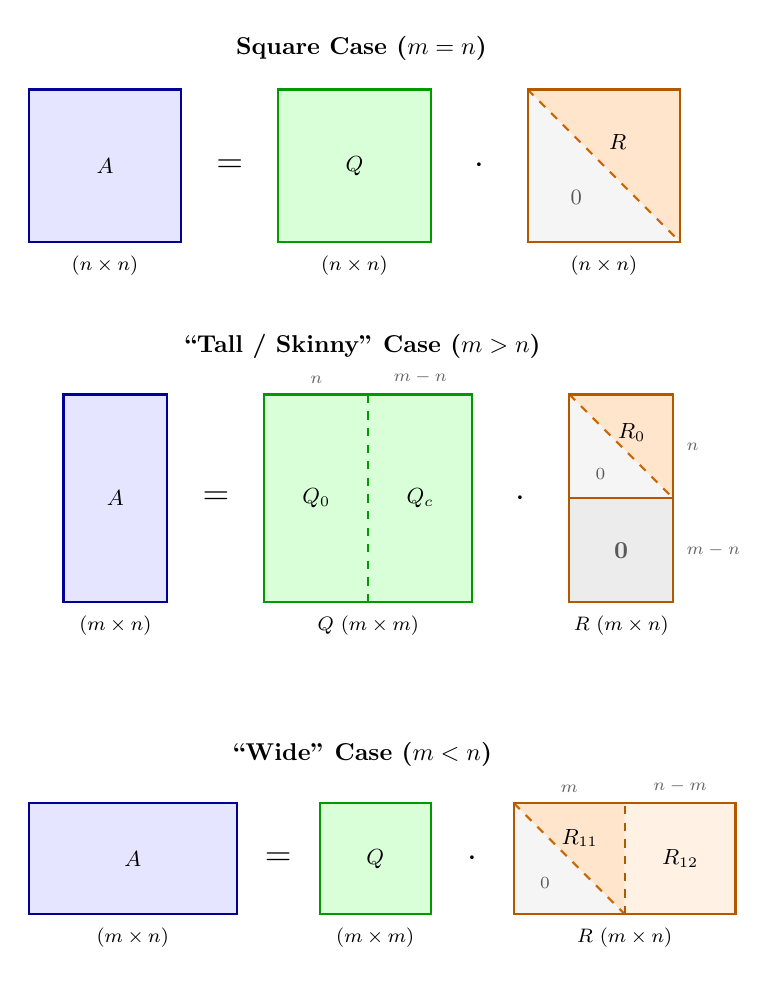
\begin{tikzpicture}[scale=0.88, every node/.style={transform shape}]
    % =========================================================
    % CASE 1: SQUARE (m = n)
    % =========================================================
    \begin{scope}[yshift=0cm]
        \node[font=\bfseries] at (5.0, 2.8) {Square Case ($m = n$)};
        
        % Matrix A (n x n)
        \draw[thick, fill=blue!10, draw=blue!60!black] (0.2, 0) rectangle (2.4, 2.2);
        \node[font=\small\bfseries] at (1.3, 1.1) {$A$};
        \node[below=2pt, font=\footnotesize] at (1.3, 0) {$(n \times n)$};
        
        % Equals sign
        \node[font=\Large\bfseries] at (3.1, 1.1) {$=$};
        
        % Matrix Q (n x n)
        \draw[thick, fill=green!15, draw=green!60!black] (3.8, 0) rectangle (6.0, 2.2);
        \node[font=\small\bfseries] at (4.9, 1.1) {$Q$};
        \node[below=2pt, font=\footnotesize] at (4.9, 0) {$(n \times n)$};
        
        % Dot sign
        \node[font=\Large\bfseries] at (6.7, 1.1) {$\cdot$};
        
        % Matrix R (n x n)
        \fill[orange!20] (7.4, 2.2) -- (9.6, 2.2) -- (9.6, 0) -- cycle;
        \fill[gray!8] (7.4, 2.2) -- (7.4, 0) -- (9.6, 0) -- cycle;
        \draw[thick, dashed, draw=orange!80!black] (7.4, 2.2) -- (9.6, 0);
        \draw[thick, draw=orange!70!black] (7.4, 0) rectangle (9.6, 2.2);
        \node[font=\small\bfseries] at (8.7, 1.45) {$R$};
        \node[font=\small, text=gray!70!black] at (8.1, 0.65) {$0$};
        \node[below=2pt, font=\footnotesize] at (8.5, 0) {$(n \times n)$};
    \end{scope}

    % =========================================================
    % CASE 2: TALL / SKINNY (m > n)
    % =========================================================
    \begin{scope}[yshift=-5.2cm]
        \node[font=\bfseries] at (5.0, 3.7) {``Tall / Skinny'' Case ($m > n$)};
        
        % Matrix A (m x n)
        \draw[thick, fill=blue!10, draw=blue!60!black] (0.7, 0) rectangle (2.2, 3.0);
        \node[font=\small\bfseries] at (1.45, 1.5) {$A$};
        \node[below=2pt, font=\footnotesize] at (1.45, 0) {$(m \times n)$};
        
        % Equals sign
        \node[font=\Large\bfseries] at (2.9, 1.5) {$=$};
        
        % Matrix Q (m x m)
        \draw[thick, fill=green!15, draw=green!60!black] (3.6, 0) rectangle (6.6, 3.0);
        \draw[thick, dashed, draw=green!60!black] (5.1, 0) -- (5.1, 3.0);
        \node[font=\small\bfseries] at (4.35, 1.5) {$Q_0$};
        \node[font=\small\bfseries] at (5.85, 1.5) {$Q_c$};
        \node[above=1pt, font=\scriptsize, text=gray!80!black] at (4.35, 3.0) {$n$};
        \node[above=1pt, font=\scriptsize, text=gray!80!black] at (5.85, 3.0) {$m-n$};
        \node[below=2pt, font=\footnotesize] at (5.1, 0) {$Q \ (m \times m)$};
        
        % Dot sign
        \node[font=\Large\bfseries] at (7.3, 1.5) {$\cdot$};
        
        % Matrix R (m x n)
        % Block R_0 (n x n upper triangular)
        \fill[orange!20] (8.0, 3.0) -- (9.5, 3.0) -- (9.5, 1.5) -- cycle;
        \fill[gray!8] (8.0, 3.0) -- (8.0, 1.5) -- (9.5, 1.5) -- cycle;
        \draw[thick, dashed, draw=orange!80!black] (8.0, 3.0) -- (9.5, 1.5);
        \node[font=\small\bfseries] at (8.9, 2.45) {$R_0$};
        \node[font=\scriptsize, text=gray!70!black] at (8.45, 1.85) {$0$};
        % Block 0 lower ((m-n) x n)
        \fill[gray!15] (8.0, 0) rectangle (9.5, 1.5);
        \node[font=\bfseries, text=gray!70!black] at (8.75, 0.75) {$\mathbf{0}$};
        % Borders and dividers
        \draw[thick, draw=orange!70!black] (8.0, 1.5) -- (9.5, 1.5);
        \draw[thick, draw=orange!70!black] (8.0, 0) rectangle (9.5, 3.0);
        \node[right=2pt, font=\scriptsize, text=gray!80!black] at (9.5, 2.25) {$n$};
        \node[right=2pt, font=\scriptsize, text=gray!80!black] at (9.5, 0.75) {$m-n$};
        \node[below=2pt, font=\footnotesize] at (8.75, 0) {$R \ (m \times n)$};
    \end{scope}

    % =========================================================
    % CASE 3: WIDE (m < n)
    % =========================================================
    \begin{scope}[yshift=-9.7cm]
        \node[font=\bfseries] at (5.0, 2.3) {``Wide'' Case ($m < n$)};
        
        % Matrix A (m x n)
        \draw[thick, fill=blue!10, draw=blue!60!black] (0.2, 0) rectangle (3.2, 1.6);
        \node[font=\small\bfseries] at (1.7, 0.8) {$A$};
        \node[below=2pt, font=\footnotesize] at (1.7, 0) {$(m \times n)$};
        
        % Equals sign
        \node[font=\Large\bfseries] at (3.8, 0.8) {$=$};
        
        % Matrix Q (m x m)
        \draw[thick, fill=green!15, draw=green!60!black] (4.4, 0) rectangle (6.0, 1.6);
        \node[font=\small\bfseries] at (5.2, 0.8) {$Q$};
        \node[below=2pt, font=\footnotesize] at (5.2, 0) {$(m \times m)$};
        
        % Dot sign
        \node[font=\Large\bfseries] at (6.6, 0.8) {$\cdot$};
        
        % Matrix R (m x n)
        % Block R_11 (m x m upper triangular)
        \fill[orange!20] (7.2, 1.6) -- (8.8, 1.6) -- (8.8, 0) -- cycle;
        \fill[gray!8] (7.2, 1.6) -- (7.2, 0) -- (8.8, 0) -- cycle;
        \draw[thick, dashed, draw=orange!80!black] (7.2, 1.6) -- (8.8, 0);
        \node[font=\small\bfseries] at (8.15, 1.1) {$R_{11}$};
        \node[font=\scriptsize, text=gray!70!black] at (7.65, 0.45) {$0$};
        % Block R_12 (m x (n-m) dense)
        \fill[orange!10] (8.8, 0) rectangle (10.4, 1.6);
        \node[font=\small\bfseries] at (9.6, 0.8) {$R_{12}$};
        % Borders and dividers
        \draw[thick, dashed, draw=orange!70!black] (8.8, 0) -- (8.8, 1.6);
        \draw[thick, draw=orange!70!black] (7.2, 0) rectangle (10.4, 1.6);
        \node[above=1pt, font=\scriptsize, text=gray!80!black] at (8.0, 1.6) {$m$};
        \node[above=1pt, font=\scriptsize, text=gray!80!black] at (9.6, 1.6) {$n-m$};
        \node[below=2pt, font=\footnotesize] at (8.8, 0) {$R \ (m \times n)$};
    \end{scope}
\end{tikzpicture}
\caption{Dimensional structure of the QR decomposition across the three geometric regimes ($m = n$, $m > n$, and $m < n$).}
\label{fig:qr-three-cases-en}
\end{figure}

\begin{enumerate}
    \item \textbf{Square matrix ($m = n$):}
    $A, Q, R \in \R^{n \times n}$. The matrix $R$ is classical upper triangular ($R_{i,j} = 0$ for $i > j$).
    \item \textbf{Wide / horizontal matrix ($m < n$):}
    $Q \in \R^{m \times m}$ is square orthogonal. The matrix $R \in \R^{m \times n}$ has zero entries below the main diagonal in its first $m$ columns ($R_{i,j} = 0$ for $i > j$), while the remaining $n - m$ columns are generally dense.
    \item \textbf{Tall and skinny matrix ($m > n$):}
    $Q \in \R^{m \times m}$ is full-order square orthogonal. The matrix $R \in \R^{m \times n}$ partitions vertically into an upper square upper-triangular block $R_0 \in \R^{n \times n}$ and a bottom block of $(m - n) \times n$ zero rows.
\end{enumerate}

\subsection{Economical QR Decomposition (Thin / Economy QR)}
In practical machine learning and data analysis applications, data matrices are typically ``tall and skinny'' ($m \gg n$, with millions of observations and tens or hundreds of features). In this setting, storing the entire orthogonal matrix $Q \in \R^{m \times m}$ requires $\BigO{m^2}$ memory cells, an impractical and unnecessary overhead.

Partitioning $Q$ by columns and $R$ by row blocks:
\begin{equation}
    Q = \begin{bmatrix} Q_0 & Q_c \end{bmatrix}, \quad Q_0 \in \R^{m \times n}, \quad Q_c \in \R^{m \times (m-n)},
\end{equation}
\begin{equation}
    R = \begin{bmatrix} R_0 \\ \mathbf{0} \end{bmatrix}, \quad R_0 \in \R^{n \times n}, \quad \mathbf{0} \in \R^{(m-n) \times n}.
\end{equation}
Evaluating the block product:
\begin{equation}
    A = Q R = \begin{bmatrix} Q_0 & Q_c \end{bmatrix} \begin{bmatrix} R_0 \\ \mathbf{0} \end{bmatrix} = Q_0 R_0 + Q_c \cdot \mathbf{0} = Q_0 R_0.
\end{equation}

\begin{definition}[Thin / Economy QR]
\label{def:thin-qr-en}
The factorization $A = Q_0 R_0$ is called \textbf{Thin QR} (or \textbf{Economy QR}):
\begin{itemize}
    \item $Q_0 \in \R^{m \times n}$ has $n$ orthonormal columns: $Q_0^T Q_0 = I_n$; however, in general $Q_0 Q_0^T \neq I_m$ (it is not a global isometry of $\R^m$, but rather the orthogonal projector onto the column space of $A$).
    \item $R_0 \in \R^{n \times n}$ is a square upper triangular matrix.
\end{itemize}
The memory footprint decreases from $\BigO{m^2}$ to $\BigO{mn}$, enabling scalability on large datasets.
\end{definition}

\FloatBarrier
\section{Fundamental Applications of QR Decomposition}
\label{sec:applications-qr-en}

The QR decomposition serves as a primary computational building block across computational disciplines:

\begin{enumerate}
    \item \textbf{Linear Least Squares Problems (Ordinary Least Squares):}
    Given an overdetermined system $Ax \approx b$ with $A \in \R^{m \times n}$ ($m \ge n$) having full column rank, the Euclidean minimization problem:
    \begin{equation}
        \min_{x \in \R^n} \|Ax - b\|_2^2
    \end{equation}
    avoids computing the ill-conditioned normal equations $A^T A x = A^T b$ (which squares the condition number: $\cond_2(A^T A) = \cond_2(A)^2$). Substituting the Thin QR decomposition $A = Q_0 R_0$, the problem reduces directly to the triangular system:
    \begin{equation}
        R_0 x = Q_0^T b,
    \end{equation}
    solvable by back substitution in $\BigO{n^2}$ flops with condition number $\cond_2(R_0) = \cond_2(A)$.
    
    \item \textbf{Spectral Eigenvalue Computation (The QR Algorithm):}
    Considered one of the top ten algorithms of the 20th century for general and symmetric matrix diagonalization, it generates an iterative sequence of orthogonally similar matrices:
    \begin{equation}
        A_k = Q_k R_k \implies A_{k+1} = R_k Q_k = Q_k^T A_k Q_k.
    \end{equation}
    Under mild conditions, $A_k$ converges asymptotically to upper triangular Schur form, revealing eigenvalues on the diagonal.

    \item \textbf{General Square Linear Systems:}
    If $Ax = b$ with non-singular $A \in \R^{n \times n}$, $A = QR$ rewrites the system as:
    \begin{equation}
        R x = Q^T b,
    \end{equation}
    replacing Gaussian elimination with partial pivoting by an orthogonally stable routine.

    \item \textbf{Orthonormal Bases for Matrix Range:}
    When $A$ has full column rank $n$, the columns of $Q_0 = [\mathbf{q}_1, \dots, \mathbf{q}_n]$ form an exact orthonormal basis for the column space of $A$:
    \begin{equation}
        \operatorname{Im}(A) = \operatorname{span}(Q_0).
    \end{equation}

    \item \textbf{Backward Numerical Stability:}
    Unlike classical Gram-Schmidt orthogonalization (which suffers from severe loss of orthogonality due to accumulated floating-point cancellations), Householder reflections guarantee that computed factors $\tilde{Q}$ and $\tilde{R}$ satisfy:
    \begin{equation}
        \tilde{Q} \tilde{R} = A + \Delta A, \quad \frac{\|\Delta A\|_2}{\|A\|_2} \le c \cdot \epsilon_{\text{mach}},
    \end{equation}
    ensuring optimal backward stability.
\end{enumerate}

\FloatBarrier
\section{Elementary Orthogonal Matrices: Introductory Problem}
\label{sec:elementary-orthogonal-matrices-en}

To construct an algorithm capable of computing the QR factorization, we analyze the class of symmetric rank-1 perturbations of the identity matrix.

\subsection{Problem Formulation}
Let $v \in \R^n$ be a unit vector ($\|v\|_2 = 1$, i.e., $v^T v = 1$) and let $\alpha \in \R$ be a real scalar parameter. Consider the square matrix:
\begin{equation}
    Q = I_n - \alpha v v^T.
    \label{eq:form-matrix-alpha-en}
\end{equation}

We address three foundational analytical questions:
\begin{enumerate}
    \item For which values of $\alpha \in \R$ is the matrix $Q$ orthogonal?
    \item For these values, what is the analytic form of the inverse $Q^{-1}$?
    \item What is the computational cost of the matrix-vector product $Q x$ for a generic vector $x \in \R^n$?
\end{enumerate}

\subsection{Orthogonality Condition: Derivation of $\alpha$}
A real square matrix $Q$ is orthogonal if and only if $Q Q^T = I$.
We first compute the transpose of $Q$:
\begin{equation}
    Q^T = (I - \alpha v v^T)^T = I^T - \alpha (v v^T)^T = I - \alpha (v^T)^T v^T = I - \alpha v v^T = Q.
\end{equation}
Hence, for any $\alpha$, the matrix $Q$ is \textbf{symmetric} ($Q^T = Q$).

Imposing the orthogonality condition:
\begin{equation}
    Q Q^T = I \iff Q^2 = I \iff (I - \alpha v v^T)(I - \alpha v v^T) = I.
\end{equation}
Expanding using distributivity:
\begin{equation}
    (I - \alpha v v^T)(I - \alpha v v^T) = I \cdot I - \alpha v v^T - \alpha v v^T + \alpha^2 (v v^T)(v v^T).
\end{equation}
Exploiting associativity in the quadratic term:
\begin{equation}
    (v v^T)(v v^T) = v (v^T v) v^T.
\end{equation}
Because $v$ is a unit vector by hypothesis, the inner scalar is $v^T v = \|v\|_2^2 = 1$. The term simplifies to:
\begin{equation}
    (v v^T)(v v^T) = v (1) v^T = v v^T.
\end{equation}
Substituting back:
\begin{equation}
    I - 2\alpha v v^T + \alpha^2 v v^T = I.
\end{equation}
Subtracting $I$ from both sides:
\begin{equation}
    -2\alpha v v^T + \alpha^2 v v^T = \mathbf{0} \iff (\alpha^2 - 2\alpha) v v^T = \mathbf{0}.
\end{equation}
Since $v \neq \mathbf{0}$, the outer product matrix $v v^T \neq \mathbf{0}$ is non-zero. Matrix equality holds if and only if the scalar coefficient vanishes:
\begin{equation}
    \alpha^2 - 2\alpha = 0 \iff \alpha(\alpha - 2) = 0 \implies \alpha = 0 \quad \text{or} \quad \alpha = 2.
\end{equation}

\begin{itemize}
    \item If $\alpha = 0$, $Q = I_n$ (the identity matrix, a trivial isometry).
    \item If $\alpha = 2$, we obtain the non-trivial transformation:
    \begin{equation}
        Q = I_n - 2 v v^T.
    \end{equation}
    This matrix is known as an \textbf{elementary reflector}.
\end{itemize}

\subsection{Matrix Inverse: The Involution Property}
Because $Q$ is simultaneously symmetric ($Q^T = Q$) and orthogonal ($Q^{-1} = Q^T$), for $\alpha = 2$ we immediately have:
\begin{equation}
    Q^{-1} = Q^T = Q.
\end{equation}
A matrix that equals its own inverse ($Q^2 = I$) is called an \textbf{involution}. Geometrically, applying a reflection twice returns any vector to its original state.

\subsection{Computational Cost of $Q x$}
For a generic vector $x \in \R^n$, we determine the operational cost to compute $y = Q x = (I - 2 v v^T) x$.

\begin{alertblock}{Optimization Principle: Never Form the Matrix Explicitly}
Explicitly constructing $Q = I - 2 v v^T$ requires computing the outer product $v v^T$ ($\BigO{n^2}$ operations) and storing $n^2$ numbers. Furthermore, subsequent dense matrix-vector multiplication $Q x$ would cost another $2n^2$ flops.
Exploiting rank-1 structure and algebraic associativity, we never materialize $Q$ as a 2D array:
\begin{equation}
    Q x = (I - 2 v v^T) x = x - 2 v (v^T x).
    \label{eq:eval-vector-householder-en}
\end{equation}
\end{alertblock}

The computation $y = Q x$ decomposes into four sequential steps:
\begin{enumerate}
    \item \textbf{Inner dot product} $\beta = v^T x = \sum_{i=1}^n v_i x_i$:\\
    Requires $n$ multiplications and $n - 1$ additions $\implies 2n - 1$ flops ($\BigO{n}$).
    \item \textbf{Scalar multiplication} $\gamma = 2 \beta$:\\
    Requires $1$ scalar multiplication $\implies 1$ flop ($\BigO{1}$).
    \item \textbf{Vector scaling} $w = \gamma v$:\\
    Requires $n$ multiplications $\implies n$ flops ($\BigO{n}$).
    \item \textbf{Vector subtraction} $y = x - w$:\\
    Requires $n$ subtractions $\implies n$ flops ($\BigO{n}$).
\end{enumerate}

\paragraph{Total operational complexity:}
\begin{equation}
    \text{Flops}(Q x) = (2n - 1) + 1 + n + n = 4n \implies \BigO{n}.
\end{equation}
Complexity drops from quadratic $\BigO{n^2}$ to strictly \textbf{linear} $\BigO{n}$.

\FloatBarrier
\section{Householder Reflectors and Fundamental Lemma}
\label{sec:householder-reflectors-lemma-en}

\subsection{General Definition of Householder Reflectors}

\begin{definition}[Householder Reflector]
\label{def:householder-reflector-en}
Let $v \in \R^n$ be any non-zero vector ($v \neq \mathbf{0}$, not necessarily normalized). The \textbf{Householder matrix} or \textbf{Householder reflector} associated with $v$ is:
\begin{equation}
    H_v = I_n - \frac{2}{\|v\|_2^2} v v^T.
    \label{eq:householder-reflector-gen-en}
\end{equation}
\end{definition}

Setting $u = \frac{v}{\|v\|_2}$ (the unit vector along $v$), note that $\frac{2}{\|v\|^2} v v^T = 2 u u^T$, recovering the elementary form from Section~\ref{sec:elementary-orthogonal-matrices-en}. Its primary properties follow immediately:
\begin{enumerate}
    \item \textbf{Symmetry:} $H_v^T = H_v$.
    \item \textbf{Orthogonality and Involution:} $H_v^T H_v = H_v^2 = I_n \implies H_v^{-1} = H_v$.
    \item \textbf{Scale Invariance:} For any non-zero real scalar $c \neq 0$, $H_{c v} = H_v$.
\end{enumerate}

\subsection{Geometric Interpretation: Hyperplane Reflection}
Consider the $(n-1)$-dimensional hyperplane $v^\perp \subset \R^n$ orthogonal to $v$:
\begin{equation}
    v^\perp = \{z \in \R^n : v^T z = 0\}.
\end{equation}
By the orthogonal decomposition theorem, any vector $x \in \R^n$ decomposes uniquely as:
\begin{equation}
    x = x_\parallel + x_\perp,
\end{equation}
where the component parallel to $v$ is the orthogonal projection onto $\operatorname{span}(v)$:
\begin{equation}
    x_\parallel = \frac{v^T x}{\|v\|^2} v,
\end{equation}
and the component lying in the hyperplane is $x_\perp = x - x_\parallel \in v^\perp$.

Applying $H_v$ to $x$:
\begin{equation}
    H_v x = x - \frac{2 v^T x}{\|v\|^2} v = (x_\parallel + x_\perp) - 2 x_\parallel = x_\perp - x_\parallel.
\end{equation}
The operator preserves the in-plane component ($x_\perp$) while reversing the orthogonal component ($x_\parallel \mapsto -x_\parallel$). Therefore, $H_v$ acts as the \textbf{orthogonal mirror reflection} across the hyperplane $v^\perp$.

\begin{figure}[H]
\centering
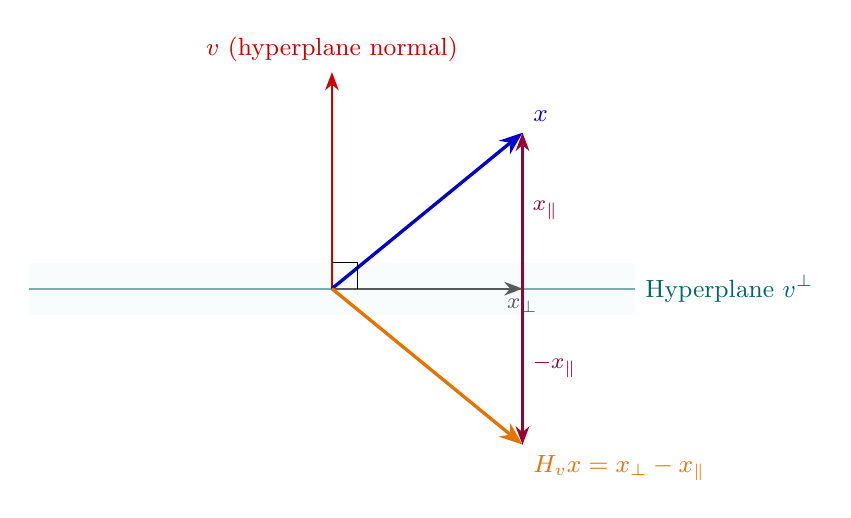
\begin{tikzpicture}[scale=1.1]
    % Hyperplane v_perp
    \draw[thick, teal!80!black] (-3.5, 0) -- (3.5, 0) node[right, font=\small] {Hyperplane $v^\perp$};
    \fill[teal!5, opacity=0.5] (-3.5, -0.3) rectangle (3.5, 0.3);

    % Normal vector v
    \draw[-Stealth, thick, red!80!black] (0, 0) -- (0, 2.5) node[above, font=\small] {$v$ (hyperplane normal)};

    % Vector x
    \coordinate (X) at (2.2, 1.8);
    \draw[-Stealth, very thick, blue!80!black] (0, 0) -- (X) node[above right, font=\small] {$x$};

    % Projections
    \coordinate (Xperp) at (2.2, 0);
    \draw[dashed, gray] (X) -- (Xperp);
    \draw[-Stealth, thick, gray!70!black] (0, 0) -- (Xperp) node[below, font=\footnotesize] {$x_\perp$};
    \draw[-Stealth, thick, purple!80!black] (Xperp) -- (X) node[right, midway, font=\footnotesize] {$x_\parallel$};

    % Reflected vector H_v(x)
    \coordinate (HX) at (2.2, -1.8);
    \draw[-Stealth, very thick, orange!90!black] (0, 0) -- (HX) node[below right, font=\small] {$H_v x = x_\perp - x_\parallel$};
    \draw[dashed, gray] (HX) -- (Xperp);
    \draw[-Stealth, thick, purple!80!black] (Xperp) -- (HX) node[right, midway, font=\footnotesize] {$-x_\parallel$};

    % Right angle
    \draw[thin] (0, 0.3) -- (0.3, 0.3) -- (0.3, 0);
\end{tikzpicture}
\caption{Geometric interpretation of a Householder reflection: specular reflection across the hyperplane $v^\perp$.}
\label{fig:householder-hyperplane-reflection-en}
\end{figure}

\subsection{Fundamental Reflection Lemma}

\begin{lemma}[Fundamental Householder Reflection Lemma]
\label{lem:fundamental-reflection-en}
Let $x, y \in \R^n$ be two distinct vectors having identical Euclidean norms:
\begin{equation}
    x \neq y \quad \text{and} \quad \|x\|_2 = \|y\|_2.
\end{equation}
Defining the Householder vector as their difference:
\begin{equation}
    v = x - y,
\end{equation}
the associated reflector $H_v$ transforms $x$ exactly into $y$:
\begin{equation}
    H_v x = y.
\end{equation}
\end{lemma}

\begin{proof}
By the definition of the Householder reflector applied to $x$:
\begin{equation}
    H_v x = x - \frac{2}{\|v\|^2} v (v^T x) = x - \frac{2}{\|x - y\|^2} (x - y) \left( (x - y)^T x \right).
    \label{eq:proof-lemma-base-en}
\end{equation}
We expand the scalar denominator and numerator independently:

\paragraph{1. Expansion of the denominator $\|x - y\|^2$:}
\begin{equation}
    \|x - y\|^2 = (x - y)^T (x - y) = x^T x - x^T y - y^T x + y^T y.
\end{equation}
Since the real inner product is commutative ($x^T y = y^T x$) and by hypothesis $\|x\|_2^2 = x^T x = y^T y = \|y\|_2^2$:
\begin{equation}
    \|x - y\|^2 = x^T x - 2 x^T y + x^T x = 2 x^T x - 2 x^T y = 2 (x^T x - x^T y).
    \label{eq:proof-denom-en}
\end{equation}

\paragraph{2. Expansion of the numerator scalar $(x - y)^T x$:}
\begin{equation}
    (x - y)^T x = x^T x - y^T x = x^T x - x^T y.
    \label{eq:proof-num-en}
\end{equation}

\paragraph{3. Substitution into the reflection operator:}
Inserting~\eqref{eq:proof-denom-en} and~\eqref{eq:proof-num-en} into~\eqref{eq:proof-lemma-base-en}:
\begin{equation}
    H_v x = x - \frac{2}{2 (x^T x - x^T y)} (x - y) (x^T x - x^T y).
\end{equation}
Since $x \neq y$ and $\|x\| = \|y\|$, Cauchy-Schwarz ensures $x^T x - x^T y > 0$, so the term is non-zero. Canceling common factors:
\begin{equation}
    H_v x = x - (x - y) = x - x + y = y.
\end{equation}
The proof is complete.
\end{proof}

\subsection{Linear Algebra Review: Inner Product vs. Outer Product}
When manipulating bilinear matrix structures, distinguish clearly between:
\begin{itemize}
    \item \textbf{Inner (dot) product:} $x^T y = y^T x \in \R$. A single commutative scalar in $\R$.
    \item \textbf{Outer (dyadic) product:} $x y^T \in \R^{n \times n}$. A rank-1 square matrix that in general does not commute: $x y^T \neq y x^T = (x y^T)^T$.
\end{itemize}

\begin{example}[Non-commutativity of the dyadic product]
Consider orthogonal vectors $x = \begin{bmatrix} 2 \\ 0 \end{bmatrix}$ and $y = \begin{bmatrix} 0 \\ 2 \end{bmatrix}$:
\begin{equation}
    x y^T = \begin{bmatrix} 2 \\ 0 \end{bmatrix} \begin{bmatrix} 0 & 2 \end{bmatrix} = \begin{bmatrix} 0 & 4 \\ 0 & 0 \end{bmatrix},
\end{equation}
whereas:
\begin{equation}
    y x^T = \begin{bmatrix} 0 \\ 2 \end{bmatrix} \begin{bmatrix} 2 & 0 \end{bmatrix} = \begin{bmatrix} 0 & 0 \\ 4 & 0 \end{bmatrix} = (x y^T)^T \neq x y^T.
\end{equation}
In contrast, their scalar dot product is symmetric: $x^T y = y^T x = 0$.
\end{example}

\FloatBarrier
\section{Reflector Choice and Numerical Stability}
\label{sec:reflector-choice-stability-en}

\subsection{Zeroing Subdiagonal Vector Elements}
In QR factorization algorithms, the operational goal is to transform a column vector $x \in \R^n$ into a scalar multiple of the first canonical basis vector $e_1 = [1, 0, \dots, 0]^T$, eliminating all subdiagonal components:
\begin{equation}
    y = \pm \|x\|_2 e_1 = \begin{bmatrix} \pm \|x\|_2 \\ 0 \\ \vdots \\ 0 \end{bmatrix}.
\end{equation}
Since $\|\pm \|x\|_2 e_1\|_2 = \|x\|_2$, the norm-preservation hypothesis of Lemma~\ref{lem:fundamental-reflection-en} is satisfied. We can construct the Householder vector:
\begin{equation}
    v = x - y = x \mp \|x\|_2 e_1 = \begin{bmatrix} x_1 \mp \|x\|_2 \\ x_2 \\ \vdots \\ x_n \end{bmatrix}.
\end{equation}
In exact arithmetic, either sign choice satisfies:
\begin{equation}
    H_v x = \pm \|x\|_2 e_1.
\end{equation}

\subsection{Catastrophic Cancellation and the Stability Criterion}
In actual computing using finite-precision floating-point arithmetic (IEEE 754 double precision with 53-bit significand and $\epsilon_{\text{mach}} \approx 1.11 \times 10^{-16}$), subtracting two nearly identical positive numbers causes severe loss of precision, known as \textbf{catastrophic cancellation}.

If $x_1 > 0$ and the minus sign is chosen, the first component of $v$ is:
\begin{equation}
    v_1 = x_1 - \|x\|_2 = x_1 - \sqrt{x_1^2 + x_2^2 + \dots + x_n^2}.
\end{equation}
If subdiagonal elements $x_2, \dots, x_n$ are very small relative to $x_1$, then $\|x\|_2 \approx x_1$, and subtracting $x_1 - \|x\|_2$ cancels out significant bits, resulting in large relative error.

\begin{noteblock}{Golden Rule of Numerical Stability for Householder Reflectors}
To eliminate cancellation, the first component of $v$ must always be formulated as a sum of quantities with the \textbf{same sign}:
\begin{itemize}
    \item If $x_1 \ge 0$, select the positive sign:
    \begin{equation}
        v = x + \|x\|_2 e_1 \implies v_1 = x_1 + \|x\|_2,
    \end{equation}
    yielding a sum of positive values ($H_v x = -\|x\|_2 e_1$).
    \item If $x_1 < 0$, select the negative sign:
    \begin{equation}
        v = x - \|x\|_2 e_1 \implies v_1 = x_1 - \|x\|_2 = -(|x_1| + \|x\|_2),
    \end{equation}
    yielding a sum of negative values ($H_v x = +\|x\|_2 e_1$).
\end{itemize}
In compact form:
\begin{equation}
    v = x + \operatorname{sign}(x_1) \|x\|_2 e_1,
    \label{eq:stable-criterion-householder-en}
\end{equation}
with the convention $\operatorname{sign}(0) = 1$. The resulting transformed vector is:
\begin{equation}
    H_v x = -\operatorname{sign}(x_1) \|x\|_2 e_1.
\end{equation}
\end{noteblock}

\subsection{Numerical Experiment}
Consider the 4D vector with one dominant component:
\begin{equation}
    x = \begin{bmatrix} 10^4 \\ 10^{-4} \\ 10^{-4} \\ 10^{-4} \end{bmatrix}.
\end{equation}
The exact Euclidean norm is:
\begin{equation}
    \|x\|_2 = \sqrt{10^8 + 3 \cdot 10^{-8}} \approx 10^4 + 1.5 \times 10^{-12}.
\end{equation}
\begin{itemize}
    \item \textbf{Incorrect choice ($v = x - \|x\|_2 e_1$):}
    \begin{equation}
        v_1 = 10^4 - (10^4 + 1.5 \times 10^{-12}) = -1.5 \times 10^{-12}.
    \end{equation}
    Severe bit cancellation occurs when computing $v_1$. Applying the computed operator $H_v$ to $x$, components 2 through 4 in $H_v x$ fail to zero out (remaining around $10^{-4}$ or $10^{-5}$).
    \item \textbf{Correct choice under the golden rule ($v = x + \|x\|_2 e_1$):}
    \begin{equation}
        v_1 = 10^4 + (10^4 + 1.5 \times 10^{-12}) = 2 \cdot 10^4 + 1.5 \times 10^{-12}.
    \end{equation}
    No cancellation occurs. Floating-point computation yields exact zeros (up to machine precision $\approx 10^{-16}$) for all subdiagonal entries.
\end{itemize}

\FloatBarrier
\section{Householder QR Factorization Algorithm}
\label{sec:householder-qr-algorithm-en}

The Householder QR algorithm reduces a matrix $A \in \R^{m \times n}$ ($m \ge n$) to upper triangular form by applying a sequence of $n - 1$ reflectors from the left:
\begin{equation}
    H_{n-1} \cdots H_2 H_1 A = R.
\end{equation}

\begin{figure}[H]
\centering
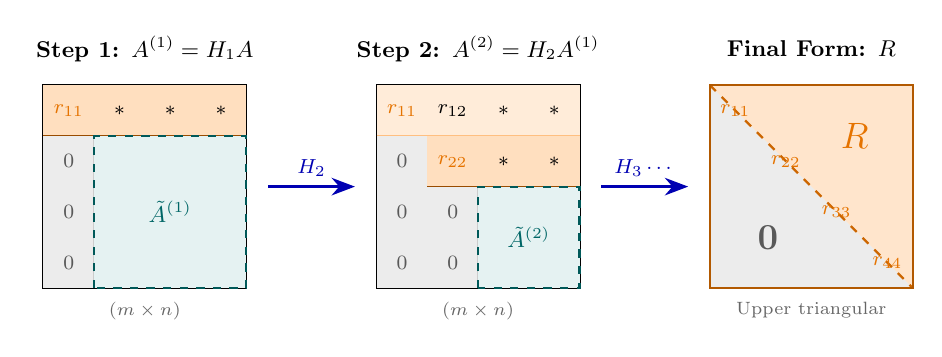
\begin{tikzpicture}[scale=0.92, every node/.style={transform shape}]
    % =========================================================
    % STEP 1: A^(1) = H_1 A
    % =========================================================
    \begin{scope}[xshift=0cm]
        \node[font=\bfseries\small] at (1.4, 3.3) {Step 1: $A^{(1)} = H_1 A$};
        
        % Outer matrix frame
        \draw[thick] (0, 0) rectangle (2.8, 2.8);
        
        % First row (modified by first reflector)
        \fill[orange!25] (0, 2.1) rectangle (2.8, 2.8);
        \draw[thick, draw=orange!60!black] (0, 2.1) -- (2.8, 2.1);
        \node[font=\footnotesize\bfseries, text=orange!90!black] at (0.35, 2.45) {$r_{11}$};
        \node[font=\footnotesize] at (1.05, 2.45) {$*$};
        \node[font=\footnotesize] at (1.75, 2.45) {$*$};
        \node[font=\footnotesize] at (2.45, 2.45) {$*$};
        
        % First column below diagonal (zeroed by H_1)
        \fill[gray!15] (0, 0) rectangle (0.7, 2.1);
        \draw[thick, draw=gray!40] (0.7, 0) -- (0.7, 2.1);
        \node[font=\footnotesize, text=gray!70!black] at (0.35, 1.75) {$0$};
        \node[font=\footnotesize, text=gray!70!black] at (0.35, 1.05) {$0$};
        \node[font=\footnotesize, text=gray!70!black] at (0.35, 0.35) {$0$};
        
        % Active submatrix tilde{A}^(1)
        \fill[teal!10] (0.7, 0) rectangle (2.8, 2.1);
        \draw[thick, dashed, draw=teal!70!black] (0.7, 0) rectangle (2.8, 2.1);
        \node[font=\small\bfseries, text=teal!80!black] at (1.75, 1.05) {$\tilde{A}^{(1)}$};
        \node[below=2pt, font=\scriptsize, text=gray!80!black] at (1.4, 0) {$(m \times n)$};
    \end{scope}

    % Arrow H_2
    \draw[-Stealth, very thick, blue!70!black] (3.1, 1.4) -- (4.3, 1.4) node[midway, above, font=\footnotesize\bfseries] {$H_2$};

    % =========================================================
    % STEP 2: A^(2) = H_2 A^(1)
    % =========================================================
    \begin{scope}[xshift=4.6cm]
        \node[font=\bfseries\small] at (1.4, 3.3) {Step 2: $A^{(2)} = H_2 A^{(1)}$};
        
        % Outer matrix frame
        \draw[thick] (0, 0) rectangle (2.8, 2.8);
        
        % First row (unchanged)
        \fill[orange!15] (0, 2.1) rectangle (2.8, 2.8);
        \draw[thick, draw=orange!50] (0, 2.1) -- (2.8, 2.1);
        \node[font=\footnotesize\bfseries, text=orange!90!black] at (0.35, 2.45) {$r_{11}$};
        \node[font=\footnotesize] at (1.05, 2.45) {$r_{12}$};
        \node[font=\footnotesize] at (1.75, 2.45) {$*$};
        \node[font=\footnotesize] at (2.45, 2.45) {$*$};
        
        % Second row (modified by tilde{H}_2)
        \fill[orange!25] (0.7, 1.4) rectangle (2.8, 2.1);
        \draw[thick, draw=orange!60!black] (0.7, 1.4) -- (2.8, 1.4);
        \node[font=\footnotesize\bfseries, text=orange!90!black] at (1.05, 1.75) {$r_{22}$};
        \node[font=\footnotesize] at (1.75, 1.75) {$*$};
        \node[font=\footnotesize] at (2.45, 1.75) {$*$};
        
        % Zeros column 1
        \fill[gray!15] (0, 0) rectangle (0.7, 2.1);
        \node[font=\footnotesize, text=gray!70!black] at (0.35, 1.75) {$0$};
        \node[font=\footnotesize, text=gray!70!black] at (0.35, 1.05) {$0$};
        \node[font=\footnotesize, text=gray!70!black] at (0.35, 0.35) {$0$};
        
        % Zeros column 2 below r_{22}
        \fill[gray!15] (0.7, 0) rectangle (1.4, 1.4);
        \draw[thick, draw=gray!40] (1.4, 0) -- (1.4, 1.4);
        \node[font=\footnotesize, text=gray!70!black] at (1.05, 1.05) {$0$};
        \node[font=\footnotesize, text=gray!70!black] at (1.05, 0.35) {$0$};
        
        % Active submatrix tilde{A}^(2)
        \fill[teal!10] (1.4, 0) rectangle (2.8, 1.4);
        \draw[thick, dashed, draw=teal!70!black] (1.4, 0) rectangle (2.8, 1.4);
        \node[font=\small\bfseries, text=teal!80!black] at (2.1, 0.7) {$\tilde{A}^{(2)}$};
        \node[below=2pt, font=\scriptsize, text=gray!80!black] at (1.4, 0) {$(m \times n)$};
    \end{scope}

    % Arrow H_3 ...
    \draw[-Stealth, very thick, blue!70!black] (7.7, 1.4) -- (8.9, 1.4) node[midway, above, font=\footnotesize\bfseries] {$H_3 \cdots$};

    % =========================================================
    % FINAL FORM: R
    % =========================================================
    \begin{scope}[xshift=9.2cm]
        \node[font=\bfseries\small] at (1.4, 3.3) {Final Form: $R$};
        
        % Upper triangle
        \fill[orange!20] (0, 2.8) -- (2.8, 2.8) -- (2.8, 0) -- cycle;
        % Lower triangle (zeros)
        \fill[gray!15] (0, 2.8) -- (0, 0) -- (2.8, 0) -- cycle;
        % Main diagonal from top-left to bottom-right
        \draw[thick, dashed, draw=orange!80!black] (0, 2.8) -- (2.8, 0);
        % Outer boundary
        \draw[thick, draw=orange!70!black] (0, 0) rectangle (2.8, 2.8);
        
        % Diagonal entries and labels
        \node[font=\footnotesize\bfseries, text=orange!90!black] at (0.35, 2.45) {$r_{11}$};
        \node[font=\footnotesize\bfseries, text=orange!90!black] at (1.05, 1.75) {$r_{22}$};
        \node[font=\footnotesize\bfseries, text=orange!90!black] at (1.75, 1.05) {$r_{33}$};
        \node[font=\footnotesize\bfseries, text=orange!90!black] at (2.45, 0.35) {$r_{44}$};
        
        \node[font=\Large\bfseries, text=orange!90!black] at (2.0, 2.1) {$R$};
        \node[font=\Large\bfseries, text=gray!70!black] at (0.8, 0.7) {$\mathbf{0}$};
        \node[below=2pt, font=\scriptsize, text=gray!80!black] at (1.4, 0) {Upper triangular};
    \end{scope}
\end{tikzpicture}
\caption{Iterative subdiagonal zeroing via the Householder QR algorithm.}
\label{fig:householder-iterations-en}
\end{figure}

\subsection{Step-by-Step Procedure}

\paragraph{Step 1:}
Extract the first column $a_1 = A_{:, 1} \in \R^m$.
\begin{enumerate}
    \item Construct the stable Householder vector:
    \begin{equation}
        v_1 = a_1 + \operatorname{sign}((a_1)_1) \|a_1\|_2 e_1 \in \R^m.
    \end{equation}
    \item Form the full-dimension reflector $H_1 = I_m - \frac{2}{\|v_1\|^2} v_1 v_1^T$.
    \item Apply the reflection to all columns of $A$:
    \begin{equation}
        A^{(1)} = H_1 A = \begin{bmatrix}
        \mp \|a_1\|_2 & * & \cdots & * \\
        0 & * & \cdots & * \\
        \vdots & \vdots & \ddots & \vdots \\
        0 & * & \cdots & *
        \end{bmatrix}.
    \end{equation}
\end{enumerate}

\paragraph{Step 2:}
To zero subdiagonal entries in the second column without destroying the zeros created in column 1, isolate the $(m-1) \times (n-1)$ active submatrix excluding row 1 and column 1.
Let $\tilde{a}_2 \in \R^{m-1}$ be the first column of this submatrix ($A^{(1)}_{2:m, 2}$).
\begin{enumerate}
    \item Define the reduced Householder vector:
    \begin{equation}
        v_2 = \tilde{a}_2 + \operatorname{sign}((\tilde{a}_2)_1) \|\tilde{a}_2\|_2 e_1 \in \R^{m-1}.
    \end{equation}
    \item Construct the reduced reflector $\hat{H}_2 \in \R^{(m-1) \times (m-1)}$:
    \begin{equation}
        \hat{H}_2 = I_{m-1} - \frac{2}{\|v_2\|^2} v_2 v_2^T.
    \end{equation}
    \item Extend $\hat{H}_2$ to full $m \times m$ dimension by block embedding:
    \begin{equation}
        H_2 = \begin{bmatrix} 1 & \mathbf{0}^T \\ \mathbf{0} & \hat{H}_2 \end{bmatrix} \in \R^{m \times m}.
    \end{equation}
    Block multiplication leaves row 1 and column 1 unaffected:
    \begin{equation}
        A^{(2)} = H_2 A^{(1)} = \begin{bmatrix} 1 & \mathbf{0}^T \\ \mathbf{0} & \hat{H}_2 \end{bmatrix} \begin{bmatrix} A^{(1)}_{1,1} & A^{(1)}_{1, 2:n} \\ \mathbf{0} & A^{(1)}_{2:m, 2:n} \end{bmatrix} = \begin{bmatrix} A^{(1)}_{1,1} & A^{(1)}_{1, 2:n} \\ \mathbf{0} & \hat{H}_2 A^{(1)}_{2:m, 2:n} \end{bmatrix}.
    \end{equation}
\end{enumerate}

\paragraph{Generic Step $k$ ($k = 1, \dots, n-1$ for $m = n$ or $k = 1, \dots, n$ for $m > n$):}
At step $k$, reflection acts solely on the bottom-right $(m - k + 1) \times (n - k + 1)$ active submatrix:
\begin{equation}
    \hat{H}_k = I_{m-k+1} - \frac{2}{\|v_k\|^2} v_k v_k^T, \qquad H_k = \begin{bmatrix} I_{k-1} & \mathbf{0} \\ \mathbf{0} & \hat{H}_k \end{bmatrix}.
\end{equation}

After $n-1$ steps (or $n$ steps if $m > n$), the resulting matrix is upper triangular:
\begin{equation}
    R = H_{n-1} \cdots H_2 H_1 A.
\end{equation}
Multiplying on the left by the inverse reflectors ($H_k^{-1} = H_k$):
\begin{equation}
    A = Q R, \quad \text{with } Q = H_1 H_2 \cdots H_{n-1}.
\end{equation}
Since every $H_k$ is orthogonal and the product of orthogonal matrices is orthogonal, $Q$ is orthogonal.

\FloatBarrier
\section{Computational Complexity and Uniqueness Properties}
\label{sec:complexity-uniqueness-qr-en}

\subsection{Computational Complexity Analysis}
During algorithm execution, updating the active submatrix at step $k$ utilizes the linear vector formula~\eqref{eq:eval-vector-householder-en} across remaining columns without explicitly forming $\hat{H}_k$:
\begin{equation}
    \hat{H}_k B = B - \frac{2}{\|v_k\|^2} v_k (v_k^T B).
\end{equation}
For a square matrix $A \in \R^{n \times n}$:
\begin{itemize}
    \item At step $k$, calculating $v_k \in \R^{n-k+1}$ takes $\approx 3(n-k)$ flops.
    \item Applying $\hat{H}_k$ to the remaining $n - k$ columns requires $4(n-k)$ flops per column, totaling $4(n-k)^2$ flops.
\end{itemize}
Summing over all $n-1$ steps:
\begin{equation}
    \text{Flops}(R) \approx \sum_{k=1}^{n-1} 4(n-k)^2 \approx 4 \int_0^n x^2 \, dx = \frac{4}{3} n^3 \ \text{flops}.
\end{equation}
If explicit accumulation of $Q = H_1 \cdots H_{n-1}$ is required, applying reflectors in reverse order starting from the identity matrix costs an additional $\frac{4}{3} n^3$ flops (totaling $\approx \frac{8}{3} n^3$ flops).

For a rectangular matrix $A \in \R^{m \times n}$ with $m \ge n$:
\begin{equation}
    \text{Flops}(R) \approx 2 m n^2 - \frac{2}{3} n^3.
\end{equation}
When $m \gg n$, the cost is asymptotically $\approx 2 m n^2$ flops.

\subsection{Uniqueness Properties of QR Factorization}
In general, the factorization $A = QR$ is \textbf{not unique}.
For any diagonal signature matrix $D = \diag(\pm 1, \dots, \pm 1) \in \R^{n \times n}$, $D$ is orthogonal and symmetric ($D = D^T = D^{-1}$), so inserting $D D = I$:
\begin{equation}
    A = Q R = (Q D) (D R) = \tilde{Q} \tilde{R}.
\end{equation}
The matrix $\tilde{Q} = Q D$ retains orthonormal columns, while $\tilde{R} = D R$ remains upper triangular with rows multiplied by $\pm 1$.

However, sign ambiguities vanish when constraining the diagonal entries of $R$:

\begin{theorem}[Conditional Uniqueness of Thin QR Factorization]
\label{thm:qr-conditional-uniqueness-en}
Let $A \in \R^{m \times n}$ with $m \ge n$ have full column rank ($\rank(A) = n$).
If all diagonal elements of $R_0$ are constrained to be strictly positive:
\begin{equation}
    (R_0)_{i,i} > 0 \quad \text{for all } i = 1, \dots, n,
\end{equation}
then the Thin QR factorization $A = Q_0 R_0$ is \textbf{strictly unique}.
\end{theorem}

\begin{proof}[Proof Sketch]
Assume two Thin QR factorizations with strictly positive diagonal elements: $A = Q_1 R_1 = Q_2 R_2$.
Computing the Gram matrix $A^T A$:
\begin{equation}
    A^T A = (Q_1 R_1)^T (Q_1 R_1) = R_1^T (Q_1^T Q_1) R_1 = R_1^T I_n R_1 = R_1^T R_1.
\end{equation}
Similarly, $A^T A = R_2^T R_2$.
Because $\rank(A) = n$, the symmetric matrix $A^T A \in \R^{n \times n}$ is strictly positive definite (SPD). By the uniqueness theorem of the \textbf{Cholesky factorization} ($M = L L^T$), there exists a unique lower triangular matrix with positive diagonal entries such that $M = L L^T$.
Identifying $L = R_1^T = R_2^T$, we immediately obtain $R_1 = R_2$.
Since $R_1$ is non-singular, multiplying on the right by $R_1^{-1}$:
\begin{equation}
    Q_1 = A R_1^{-1} = A R_2^{-1} = Q_2.
\end{equation}
Thus $Q_1 = Q_2$ and $R_1 = R_2$, proving uniqueness.
\end{proof}

\FloatBarrier
\section[Detailed Numerical Example (3x3)]{Detailed Numerical Example (\texorpdfstring{$3 \times 3$}{3x3})}
\label{sec:numerical-example-3x3-en}

\begin{example}[Complete Householder QR Factorization of a $3 \times 3$ Matrix]
Consider the real matrix:
\begin{equation}
    A = \begin{bmatrix} 
    4 & -5 & -4 \\ 
    3 & 0 & 2 \\ 
    0 & 4 & -3 
    \end{bmatrix}.
\end{equation}
We compute the factorization $A = QR$, explicitly evaluating all reflectors.

\paragraph{Step 1: Zeroing the first column}
\begin{enumerate}
    \item \textbf{First column extraction:}
    \begin{equation}
        a_1 = \begin{bmatrix} 4 \\ 3 \\ 0 \end{bmatrix}.
    \end{equation}
    \item \textbf{Euclidean norm computation:}
    \begin{equation}
        \|a_1\|_2 = \sqrt{4^2 + 3^2 + 0^2} = \sqrt{16 + 9 + 0} = \sqrt{25} = 5.
    \end{equation}
    \item \textbf{Householder vector $v_1$ construction:}
    Since $(a_1)_1 = 4 > 0$, we select the $+$ sign per equation~\eqref{eq:stable-criterion-householder-en}:
    \begin{equation}
        v_1 = a_1 + \|a_1\|_2 e_1 = \begin{bmatrix} 4 \\ 3 \\ 0 \end{bmatrix} + \begin{bmatrix} 5 \\ 0 \\ 0 \end{bmatrix} = \begin{bmatrix} 9 \\ 3 \\ 0 \end{bmatrix}.
    \end{equation}
    \item \textbf{Squared norm of $v_1$:}
    \begin{equation}
        \|v_1\|_2^2 = 9^2 + 3^2 + 0^2 = 81 + 9 + 0 = 90.
    \end{equation}
    \item \textbf{Householder matrix $H_1$ construction:}
    \begin{equation}
        H_1 = I_3 - \frac{2}{\|v_1\|^2} v_1 v_1^T = I_3 - \frac{2}{90} \begin{bmatrix} 9 \\ 3 \\ 0 \end{bmatrix} \begin{bmatrix} 9 & 3 & 0 \end{bmatrix}.
    \end{equation}
    Expanding the dyadic product:
    \begin{equation}
        \frac{2}{90} v_1 v_1^T = \frac{1}{45} \begin{bmatrix} 81 & 27 & 0 \\ 27 & 9 & 0 \\ 0 & 0 & 0 \end{bmatrix} = \begin{bmatrix} 9/5 & 3/5 & 0 \\ 3/5 & 1/5 & 0 \\ 0 & 0 & 0 \end{bmatrix}.
    \end{equation}
    Subtracting from $I_3$:
    \begin{equation}
        H_1 = \begin{bmatrix} 1 & 0 & 0 \\ 0 & 1 & 0 \\ 0 & 0 & 1 \end{bmatrix} - \begin{bmatrix} 9/5 & 3/5 & 0 \\ 3/5 & 1/5 & 0 \\ 0 & 0 & 0 \end{bmatrix} = \begin{bmatrix} -4/5 & -3/5 & 0 \\ -3/5 & 4/5 & 0 \\ 0 & 0 & 1 \end{bmatrix}.
    \end{equation}
    \item \textbf{Product $A^{(1)} = H_1 A$:}
    \begin{itemize}
        \item \textit{First column:} By construction:
        \begin{equation}
            H_1 \begin{bmatrix} 4 \\ 3 \\ 0 \end{bmatrix} = \begin{bmatrix} -\|a_1\|_2 \\ 0 \\ 0 \end{bmatrix} = \begin{bmatrix} -5 \\ 0 \\ 0 \end{bmatrix}.
        \end{equation}
        Direct algebraic verification:
        \begin{align*}
            (-4/5)(4) + (-3/5)(3) &= -\frac{16+9}{5} = -5, \\
            (-3/5)(4) + (4/5)(3) &= -\frac{12}{5} + \frac{12}{5} = 0.
        \end{align*}
        \item \textit{Second column:}
        \begin{equation}
            H_1 \begin{bmatrix} -5 \\ 0 \\ 4 \end{bmatrix} = \begin{bmatrix} (-4/5)(-5) + (-3/5)(0) \\ (-3/5)(-5) + (4/5)(0) \\ 1(4) \end{bmatrix} = \begin{bmatrix} 4 \\ 3 \\ 4 \end{bmatrix}.
        \end{equation}
        \item \textit{Third column:}
        \begin{equation}
            H_1 \begin{bmatrix} -4 \\ 2 \\ -3 \end{bmatrix} = \begin{bmatrix} (-4/5)(-4) + (-3/5)(2) \\ (-3/5)(-4) + (4/5)(2) \\ 1(-3) \end{bmatrix} = \begin{bmatrix} 2 \\ 4 \\ -3 \end{bmatrix}.
        \end{equation}
    \end{itemize}
    The transformed matrix after Step 1 is:
    \begin{equation}
        A^{(1)} = H_1 A = \begin{bmatrix} 
        -5 & 4 & 2 \\ 
        0 & 3 & 4 \\ 
        0 & 4 & -3 
        \end{bmatrix}.
    \end{equation}
\end{enumerate}

\paragraph{Step 2: Zeroing the second column}
\begin{enumerate}
    \item \textbf{Isolating the active $2 \times 2$ submatrix:}
    Rows 2--3 and columns 2--3 of $A^{(1)}$:
    \begin{equation}
        \begin{bmatrix} 3 & 4 \\ 4 & -3 \end{bmatrix}.
    \end{equation}
    The subdiagonal vector to zero is:
    \begin{equation}
        \tilde{a}_2 = \begin{bmatrix} 3 \\ 4 \end{bmatrix}.
    \end{equation}
    \item \textbf{Euclidean norm computation:}
    \begin{equation}
        \|\tilde{a}_2\|_2 = \sqrt{3^2 + 4^2} = \sqrt{9 + 16} = \sqrt{25} = 5.
    \end{equation}
    \item \textbf{Householder vector $v_2$ construction:}
    Since $(\tilde{a}_2)_1 = 3 > 0$, we choose the $+$ sign:
    \begin{equation}
        v_2 = \tilde{a}_2 + \|\tilde{a}_2\|_2 e_1 = \begin{bmatrix} 3 \\ 4 \end{bmatrix} + \begin{bmatrix} 5 \\ 0 \end{bmatrix} = \begin{bmatrix} 8 \\ 4 \end{bmatrix}.
    \end{equation}
    \item \textbf{Squared norm of $v_2$:}
    \begin{equation}
        \|v_2\|_2^2 = 8^2 + 4^2 = 64 + 16 = 80.
    \end{equation}
    \item \textbf{Reduced reflector $\hat{H}_2 \in \R^{2 \times 2}$ construction:}
    \begin{align}
        \hat{H}_2 &= I_2 - \frac{2}{\|v_2\|^2} v_2 v_2^T = I_2 - \frac{2}{80} \begin{bmatrix} 8 \\ 4 \end{bmatrix} \begin{bmatrix} 8 & 4 \end{bmatrix} \nonumber\\
        &= I_2 - \frac{1}{40} \begin{bmatrix} 64 & 32 \\ 32 & 16 \end{bmatrix} = \begin{bmatrix} 1 & 0 \\ 0 & 1 \end{bmatrix} - \begin{bmatrix} 8/5 & 4/5 \\ 4/5 & 2/5 \end{bmatrix} \nonumber\\
        &= \begin{bmatrix} -3/5 & -4/5 \\ -4/5 & 3/5 \end{bmatrix}.
    \end{align}
    \item \textbf{Embedding into full order $H_2 \in \R^{3 \times 3}$:}
    \begin{equation}
        H_2 = \begin{bmatrix} 
        1 & 0 & 0 \\ 
        0 & -3/5 & -4/5 \\ 
        0 & -4/5 & 3/5 
        \end{bmatrix}.
    \end{equation}
    \item \textbf{Final triangular matrix $R = H_2 A^{(1)}$ computation:}
    \begin{itemize}
        \item Row 1 and column 1 remain unchanged:
        \begin{equation}
            R_{1, :} = \begin{bmatrix} -5 & 4 & 2 \end{bmatrix}, \qquad R_{:, 1} = \begin{bmatrix} -5 \\ 0 \\ 0 \end{bmatrix}.
        \end{equation}
        \item The second column (rows 2--3) becomes:
        \begin{equation}
            \hat{H}_2 \begin{bmatrix} 3 \\ 4 \end{bmatrix} = \begin{bmatrix} -\|\tilde{a}_2\|_2 \\ 0 \end{bmatrix} = \begin{bmatrix} -5 \\ 0 \end{bmatrix}.
        \end{equation}
        \item The third column (rows 2--3) is given by:
        \begin{align}
            \hat{H}_2 \begin{bmatrix} 4 \\ -3 \end{bmatrix} &= \begin{bmatrix} (-3/5)(4) + (-4/5)(-3) \\ (-4/5)(4) + (3/5)(-3) \end{bmatrix} \nonumber\\
            &= \begin{bmatrix} -12/5 + 12/5 \\ -16/5 - 9/5 \end{bmatrix} = \begin{bmatrix} 0 \\ -5 \end{bmatrix}.
        \end{align}
    \end{itemize}
    We obtain the upper triangular matrix $R$:
    \begin{equation}
        R = \begin{bmatrix} 
        -5 & 4 & 2 \\ 
        0 & -5 & 0 \\ 
        0 & 0 & -5 
        \end{bmatrix}.
    \end{equation}
    \item \textbf{Orthogonal matrix $Q = H_1 H_2$ computation:}
    \begin{align}
        Q &= \begin{bmatrix} 
        -4/5 & -3/5 & 0 \\ 
        -3/5 & 4/5 & 0 \\ 
        0 & 0 & 1 
        \end{bmatrix}
        \begin{bmatrix} 
        1 & 0 & 0 \\ 
        0 & -3/5 & -4/5 \\ 
        0 & -4/5 & 3/5 
        \end{bmatrix} \nonumber\\
        &= \begin{bmatrix} 
        -4/5 & 9/25 & 12/25 \\ 
        -3/5 & -12/25 & -16/25 \\ 
        0 & -4/5 & 3/5 
        \end{bmatrix}.
    \end{align}
\end{enumerate}

\paragraph{Product Verification $Q R$:}
\begin{align}
    Q R &= \begin{bmatrix} 
    -4/5 & 9/25 & 12/25 \\ 
    -3/5 & -12/25 & -16/25 \\ 
    0 & -4/5 & 3/5 
    \end{bmatrix}
    \begin{bmatrix} 
    -5 & 4 & 2 \\ 
    0 & -5 & 0 \\ 
    0 & 0 & -5 
    \end{bmatrix} \nonumber\\[6pt]
    &= \begin{bmatrix}
    4 & -16/5 - 9/5 & -8/5 - 12/5 \\
    3 & -12/5 + 12/5 & -6/5 + 16/5 \\
    0 & 4 & -3
    \end{bmatrix}
    = \begin{bmatrix} 
    4 & -5 & -4 \\ 
    3 & 0 & 2 \\ 
    0 & 4 & -3 
    \end{bmatrix} = A.
\end{align}
Furthermore, $Q^T Q = I_3$, verifying the exactness of the computed factorization.
\end{example}

\FloatBarrier
\section{Synoptic Summary Table}
\label{sec:synoptic-summary-qr-en}

\begin{table}[H]
\centering
\small
\renewcommand{\arraystretch}{1.18}
\begin{tabularx}{\linewidth}{>{\raggedright\arraybackslash}p{3.0cm} Y Y}
\toprule
\textbf{Concept} & \textbf{Definition / Formula} & \textbf{Properties / Complexity} \\
\midrule
\textbf{Full QR} & $A = QR$, with $Q \in \R^{m \times m}$ and $R \in \R^{m \times n}$. & $Q$ orthogonal ($Q^T Q = I_m$), $R$ extended upper triangular. \\
\textbf{Thin (Economy) QR} & $A = Q_0 R_0$, with $Q_0 \in \R^{m \times n}$ and $R_0 \in \R^{n \times n}$ ($m \ge n$). & $Q_0^T Q_0 = I_n$; memory footprint $\BigO{mn}$ vs $\BigO{m^2}$; cost $\approx 2mn^2$ flops if $m \gg n$. \\
\textbf{Householder Reflector} & $H_v = I - \frac{2}{\|v\|^2} v v^T$, with $v \neq \mathbf{0}$. & Symmetric ($H_v^T = H_v$), orthogonal, involutory ($H_v^{-1} = H_v$). \\
\textbf{Product $H_v x$} & $H_v x = x - \frac{2(v^T x)}{\|v\|^2} v$. & Complexity $\BigO{n}$ flops instead of $\BigO{n^2}$, without materializing $H_v$. \\
\textbf{Reflection Lemma} & $\|x\|_2 = \|y\|_2, \ v = x - y \implies H_v x = y$. & Maps equal-norm vectors via orthogonal reflection across $v^\perp$. \\
\textbf{Stable Vector $v$} & $v = x + \operatorname{sign}(x_1) \|x\|_2 e_1$. & Eliminates numerical cancellation, ensures backward stability. \\
\textbf{Householder QR Cost} & $H_{n-1} \cdots H_1 A = R$. & $\approx \frac{4}{3} n^3$ flops for $A \in \R^{n \times n}$; $\approx 2mn^2 - \frac{2}{3}n^3$ flops for $m \times n$. \\
\textbf{Uniqueness Theorem} & Unique if $\rank(A) = n$ and $(R_0)_{i,i} > 0$. & Connected to Cholesky uniqueness on $A^T A = R_0^T R_0$. \\
\bottomrule
\end{tabularx}
\caption{Synoptic comparative overview of QR factorization and Householder reflections.}
\label{tab:synoptic-summary-qr-en}
\end{table}


% ========================================================
% PART II: CONTINUOUS OPTIMIZATION AND MACHINE LEARNING
% ========================================================
\part{Continuous Optimization and Machine Learning}
\chapter{Elementary Univariate Optimization Problems}
\label{chap:simple-optimization-problems}

\FloatBarrier
\section{Introduction, Motivation, and Learning Objectives}
\label{sec:opt-intro-motivation}

Mathematical optimization constitutes, alongside numerical linear algebra, the second computational pillar of machine learning and data science~\cite{boyd2004convex,nocedal2006numerical}. In practical machine learning pipelines, virtually every model---from linear regression to deep neural architectures parameterizing hundreds of billions of weights---is conceptually formalized as the minimization of an empirical loss augmented by regularizing penalties over a designated admissible domain:
\begin{equation}
\min_{w \in \mathcal{W}} \mathcal{L}(w; \mathcal{D}) + \lambda \Omega(w)
\end{equation}
where $\mathcal{L}$ represents the empirical loss over dataset $\mathcal{D}$, $\Omega$ imposes geometric regularization, and $\mathcal{W}$ delimits the feasible parameter set.

However, generic non-linear optimization is an intrinsically intractable endeavor: devoid of structural assumptions, locating the global minimum of an arbitrary function is formally unsolvable within finite time. To build a robust computational foundation, the pedagogical methodology adopted in this second part of the course follows an incremental, modular paradigm:
\begin{enumerate}
    \item \textbf{Elementary univariate problem analysis:} examining linear and quadratic functions over $\R$, endowed with analytical structures so transparent that they admit closed-form solutions with $\BigO{1}$ computational complexity.
    \item \textbf{Developing geometric and algebraic intuition:} gaining deep insight into gradients, curvatures, level sets, and the active influence of boundary constraints.
    \item \textbf{Identifying boundaries of computational tractability:} understanding precisely how relaxing a structural assumption or expanding into multidimensional spaces transforms elementary decisions into NP-hard challenges.
    \item \textbf{Simple problems as algorithmic building blocks:} in virtually all state-of-the-art algorithms for non-linear and large-scale optimization (such as Newton, Quasi-Newton, Sequential Quadratic Programming, and line search techniques), the inner computational core repeatedly solves an elementary local approximation (linear or quadratic) of the complex global objective.
\end{enumerate}

\begin{noteblock}{Methodological Philosophy}
Mastering univariate linear and quadratic optimization is not merely an introductory exercise: it represents the foundational vocabulary in which advanced numerical algorithms for modern machine learning are written.
\end{noteblock}


\FloatBarrier
\section{Fundamental Definitions: Spaces, Functions, Graphs, and Level Sets}
\label{sec:opt-fundamental-definitions}

\subsection{Input and Output Spaces}
Consider the simplest scalar unconstrained setting:
\begin{itemize}
    \item \textbf{Input space:} $x \in \R$
    \item \textbf{Output space:} $y \in \R$
\end{itemize}
A scalar mapping $f: \R \to \R$ assigns to each input value $x$ a unique real output $y = f(x)$.

\subsection{Graph of a Function}
\begin{definition}[Graph]
Given a scalar function $f: \R \to \R$, the \textbf{graph} of $f$, denoted by $\operatorname{gr}(f)$, is the subset of the two-dimensional Cartesian product space $\R^2$ defined as:
\begin{equation}
\operatorname{gr}(f) = \left\{ (x, f(x)) \in \R^2 : x \in \R \right\} \subset \R^2
\end{equation}
\end{definition}
Geometrically, for univariate functions, $\operatorname{gr}(f)$ traces a planar curve in the $(x, y)$ coordinate plane.

\subsection{Image (Effective Codomain)}
\begin{definition}[Image]
The \textbf{image} of a function $f$, denoted by $\operatorname{im}(f)$, is the set of all real output values achieved by the mapping:
\begin{equation}
\operatorname{im}(f) = \left\{ y \in \R : \exists x \in \R \text{ such that } y = f(x) \right\} = f(\R) \subseteq \R
\end{equation}
\end{definition}
Geometrically, $\operatorname{im}(f)$ corresponds to the orthogonal projection of the graph $\operatorname{gr}(f)$ onto the vertical ordinate axis ($y$-axis).

\subsection{Level Sets and Sublevel Sets}
\begin{definition}[Level Set]
Given a target value $v \in \R$, the \textbf{level set} at value $v$, denoted by $L(f, v)$, is the pre-image of $v$ within the domain:
\begin{equation}
L(f, v) = \left\{ x \in \R : f(x) = v \right\} \subset \R
\end{equation}
\end{definition}

The geometric interpretation is direct: $L(f, v)$ represents the intersection between the curve $\operatorname{gr}(f)$ and the horizontal line $y = v$, projected onto the abscissa axis ($x$-axis).

\begin{remark}[Roots or Zeros of a Function]
The special case where $v = 0$ identifies the set of roots of the function:
\begin{equation}
\operatorname{roots}(f) = L(f, 0) = \{ x \in \R : f(x) = 0 \}
\end{equation}
\end{remark}

\begin{definition}[Sublevel Set]
Given a threshold $v \in \R$, the \textbf{sublevel set} at level $v$, denoted by $S(f, v)$, is defined as:
\begin{equation}
S(f, v) = \left\{ x \in \R : f(x) \le v \right\} \subset \R
\end{equation}
\end{definition}
Sublevel sets play a central role in convexity characterizations and convergence proofs for descent algorithms.


\FloatBarrier
\section{The Unconstrained Univariate Optimization Problem}
\label{sec:opt-unconstrained-problem}

\subsection{Formal Problem Statement}
Given an objective function $f: \R \to \R$, the unconstrained univariate minimization problem is formally stated as:
\begin{equation}
(P) \quad f^* = \min \{ f(x) : x \in \R \}
\end{equation}

\subsection{Optimal Value vs Optimal Solution}
A rigorous conceptual distinction must be maintained between the optimal value and an optimal minimizer:

\begin{definition}[Optimal Value]
The \textbf{optimal value} (denoted by $f^* \in \R$ or $\nu(P)$) is the scalar representing the infimum achieved by the image of the objective function:
\begin{equation}
f^* = \min(\operatorname{im}(f)) = \min \{ v \in \R : L(f, v) \neq \emptyset \}
\end{equation}
If the minimum exists, the optimal value $f^*$ is \textbf{strictly unique}.
\end{definition}

\begin{definition}[Optimal Solution or Minimizer]
An \textbf{optimal solution} (denoted by $x^*$) is a point in the domain $x^* \in \R$ at which the function attains its optimal value:
\begin{equation}
f(x^*) = f^* \quad \Longleftrightarrow \quad f(x^*) \le f(x), \quad \forall x \in \R
\end{equation}
The set of all minimizers is denoted using the set-valued $\argmin$ operator:
\begin{equation}
X^* = \argmin \{ f(x) : x \in \R \} = L(f, f^*)
\end{equation}
\end{definition}

\begin{property}[Non-Uniqueness of Minimizers]
While the optimal value $f^*$ is always a unique scalar, the set of minimizers $X^*$ may:
\begin{enumerate}
    \item Be empty ($X^* = \emptyset$, when the minimum is not attained).
    \item Contain a single isolated point ($|X^*| = 1$, unique global minimizer).
    \item Contain a discrete set of multiple points (e.g., $f(x) = \sin(x)$ with $f^* = -1$ and $X^* = \{ -\pi/2 + 2k\pi : k \in \mathbb{Z} \}$).
    \item Contain a continuum of points (e.g., a constant function over an interval).
\end{enumerate}
\end{property}

\subsection{Indifference Between Equivalent Minimizers}
From an optimization perspective:
\begin{equation}
\forall x_1^*, x_2^* \in X^* \implies f(x_1^*) = f(x_2^*) = f^*
\end{equation}
All points within $X^*$ are perfectly indistinguishable to the objective function. Barring secondary criteria or explicit regularizations (such as minimal $\ell_2$-norm or $\ell_1$-sparsity preferences), any numerical solver is mathematically authorized to return an arbitrary element of $X^*$.


\FloatBarrier
\section{Simple Reformulations and Equivalence}
\label{sec:opt-reformulations-equivalence}

Two optimization problems are termed \textbf{equivalent} if solving one directly yields the solution of the other without requiring non-trivial iterative computations.

\subsection{Min--Max Duality}
Without loss of generality (w.l.o.g.), optimization theory can be formulated strictly in terms of minimization problems. Any maximization problem can be transformed by negating the objective function:
\begin{align}
\min \{ f(x) : x \in \R \} &= - \max \{ -f(x) : x \in \R \} \\
\argmin \{ f(x) : x \in \R \} &= \argmax \{ -f(x) : x \in \R \}
\end{align}

\begin{alertblock}{Conceptual Caution}
Do not confuse this equivalence with the relationship between $\min f(x)$ and $\max f(x)$: minimizing $f(x)$ and maximizing $f(x)$ are fundamentally distinct problems with opposite convexity and curvature properties. The equivalence holds exclusively between minimizing $f(x)$ and maximizing $-f(x)$.
\end{alertblock}

\subsection{Invariance Under Vertical Shifts (Additive Constant)}
Adding an arbitrary real constant $c \in \R$ shifts the graph vertically along the ordinate axis:
\begin{align}
\min \{ f(x) + c : x \in \R \} &= \min \{ f(x) : x \in \R \} + c = f^* + c \\
\argmin \{ f(x) + c : x \in \R \} &= \argmin \{ f(x) : x \in \R \} = X^*
\end{align}
The optimal value shifts by $c$, while the set of optimal minimizers $X^*$ remains invariant.

\subsection{Invariance Under Positive Scaling (Multiplicative Constant)}
Multiplying the objective by a strictly positive scalar $c > 0$ vertically dilates or compresses the graph:
\begin{align}
\min \{ c \cdot f(x) : x \in \R \} &= c \cdot \min \{ f(x) : x \in \R \} = c f^* \quad (c > 0) \\
\argmin \{ c \cdot f(x) : x \in \R \} &= \argmin \{ f(x) : x \in \R \} = X^*
\end{align}
If $c < 0$, the negative scalar inverts the orientation, turning minimization into maximization:
\begin{equation}
\min \{ c \cdot f(x) : x \in \R \} = c \cdot \max \{ f(x) : x \in \R \} = - |c| \max \{ f(x) : x \in \R \}
\end{equation}


\FloatBarrier
\section{Constrained Optimization and the Feasible Region}
\label{sec:opt-constrained-feasible-region}

\subsection{General Formulation of Constrained Optimization}
In engineering applications and machine learning, decision parameters are bounded by physical limitations, resource budgets, or algorithmic stability bounds. We define the \textbf{feasible region} $X \subseteq \R$:
\begin{equation}
(P_X) \quad f^* = \min \{ f(x) : x \in X \}
\end{equation}
\begin{itemize}
    \item A point $x \in X$ is a \textbf{feasible solution}.
    \item A point $x \in \R \setminus X$ is an \textbf{infeasible solution}.
    \item The constrained optimal value is $f^* = \min(\operatorname{im}(X, f)) = \min \{ f(x) : x \in X \}$.
    \item The constrained optimal solution set is given by:
    \begin{equation}
    X^* = L(f, f^*) \cap X
    \end{equation}
\end{itemize}

\subsection{Monotone Non-Improvement Under Constraint Restriction}
\begin{theorem}[Fundamental Constraint Inequality]
Let $X_1 \subseteq X_2 \subseteq \R$ be nested feasible regions. Then:
\begin{equation}
\min_{x \in X_1} f(x) \ge \min_{x \in X_2} f(x)
\end{equation}
In particular, for any constrained set $X \subseteq \R$:
\begin{equation}
\min_{x \in X} f(x) \ge \min_{x \in \R} f(x)
\end{equation}
\end{theorem}
\begin{proof}
Let $x_1^* \in \argmin_{x \in X_1} f(x)$. Since $X_1 \subseteq X_2$, it follows that $x_1^* \in X_2$. By definition of global minimization over $X_2$, $f(x) \ge \min_{z \in X_2} f(z)$ for any $x \in X_2$. Evaluating at $x = x_1^*$ completes the proof.
\end{proof}

\begin{noteblock}{Operational Insight}
Imposing additional constraints can never improve the optimal objective value in a minimization problem; it can only leave it unchanged or worsen it (i.e., increase it).
\end{noteblock}

\subsection{Taxonomy of Redundant Constraints}
Given a constrained problem $\min_{x \in X} f(x)$ with unconstrained minimizer set $X^*_{\text{free}} = \argmin_{x \in \R} f(x)$:
\begin{itemize}
    \item \textbf{Completely redundant (inactive) constraint:} occurs when $X^*_{\text{free}} \subseteq X$. The constrained optimal value equals the unconstrained value ($f^*_X = f^*_{\R}$) and the set of optimal solutions is unchanged.
    \item \textbf{Partially redundant constraint:} occurs when $X^*_{\text{free}} \cap X \neq \emptyset$, but $X^*_{\text{free}} \not\subseteq X$. The constraint eliminates some alternative optimal solutions without worsening the optimal value ($f^*_X = f^*_{\R}$ remains intact, while $X^*_X \subset X^*_{\text{free}}$ shrinks).
    \item \textbf{Active and essential constraint:} occurs when $X^*_{\text{free}} \cap X = \emptyset$. The constraint forces the solution onto the boundary of $X$, strictly increasing the optimal value ($f^*_X > f^*_{\R}$).
\end{itemize}

\subsection{Functional Representation of Feasible Sets}
In computational practice, the set $X$ is not defined as an abstract collection, but via systems of algebraic equations and inequalities based on constraint functions $g_i: \R \to \R$:
\begin{enumerate}
    \item \textbf{Equality Constraints:}
    \begin{equation}
    g(x) = v \quad \Longleftrightarrow \quad X = L(g, v)
    \end{equation}
    In canonical homogeneous form:
    \begin{equation}
    g(x) = 0
    \end{equation}
    \item \textbf{Inequality Constraints:}
    \begin{equation}
    g(x) \le v \quad \Longleftrightarrow \quad X = S(g, v) = \{ x \in \R : g(x) \le v \}
    \end{equation}
    In canonical normalized form:
    \begin{equation}
    g(x) \le 0
    \end{equation}
    When the constraint is originally given as $g(x) \ge 0$, multiplying by $-1$ recovers the canonical format $-g(x) \le 0$.
    \item \textbf{Conjunction of Multiple Constraints:}
    Multiple constraints correspond to the intersection of their respective sublevel sets:
    \begin{equation}
    \begin{cases} g_1(x) \le 0 \\ g_2(x) \le 0 \end{cases} \quad \Longleftrightarrow \quad X = S(g_1, 0) \cap S(g_2, 0)
    \end{equation}
    \item \textbf{Box Constraints (Closed Intervals):}
    Representing the fundamental class in univariate optimization:
    \begin{equation}
    x_- \le x \le x_+ \quad \Longleftrightarrow \quad X = [x_-, x_+]
    \end{equation}
    which is canonicalized as the two-inequality system:
    \begin{equation}
    \begin{cases} x - x_+ \le 0 \\ x_- - x \le 0 \end{cases}
    \end{equation}
\end{enumerate}


\FloatBarrier
\section{Why Optimization is Difficult: Theory vs Computational Practice}
\label{sec:opt-difficulty-theory-practice}

\subsection{Modes of Non-Existence of the Minimum}
An optimization problem can fail to admit an optimal minimizer due to two distinct topological reasons:

\subsubsection{Case 1: Unbounded Below Problem ($f^* = -\infty$)}
The objective decreases indefinitely across the domain:
\begin{equation}
\forall M \in \R, \quad \exists x \in X \quad \text{such that} \quad f(x) \le M
\end{equation}
A canonical example is $f(x) = x$ as $x \to -\infty$. In this setting, we write $f^* = -\infty$ and $\argmin f(x) = \emptyset$.

\subsubsection{Case 2: Finite Infimum Not Attained ($f^*$ finite, but $x^* \notin X$)}
The image $\operatorname{im}(f)$ is bounded below in $\R$, but the infimum does not belong to the image:
\begin{equation}
\inf \{ f(x) : x \in X \} > -\infty \quad \text{yet} \quad \nexists x^* \in X \text{ such that } f(x^*) = \inf_{x \in X} f(x)
\end{equation}
Two typical manifestations include:
\begin{itemize}
    \item \textbf{Smooth asymptotic settings:} $f(x) = e^x$ on $X = \R$. The infimum is $\inf_{x \in \R} e^x = 0$, but $e^x = 0$ has no finite solution in $\R$. The minimum is approached only asymptotically as $x \to -\infty$.
    \item \textbf{Discontinuous pathological settings:}
    \begin{equation}
    f(x) = \begin{cases} 1 & \text{if } x = 0 \\ |x| & \text{if } x \neq 0 \end{cases}
    \end{equation}
    The infimum is $0$, but at the natural candidate $x = 0$ the function jumps to $1$. No point attains $f(x) = 0$.
\end{itemize}

\subsection[Formalization via Extended Real Numbers]{Formalization via Extended Real Numbers $\overline{\R}$}
To mathematically handle these asymptotic limits, real space is extended by incorporating infinity:
\begin{equation}
\overline{\R} = \R \cup \{-\infty, +\infty\}
\end{equation}
In $\overline{\R}$, every subset $S \subseteq \R$ \textbf{always} possesses both an infimum and a supremum:
\begin{align}
\inf S &= \max \{ v \in \overline{\R} : v \le s, \; \forall s \in S \} \\
\sup S &= \min \{ v \in \overline{\R} : v \ge s, \; \forall s \in S \}
\end{align}
With empty set conventions:
\begin{equation}
\inf \emptyset = +\infty, \quad \sup \emptyset = -\infty
\end{equation}

\subsection[Optimization in Floating-Point Arithmetic]{Optimization in Finite-Precision Floating-Point Arithmetic}
In computational hardware (modern CPUs and GPUs), the continuous real line $\R$ does not exist: algorithms operate strictly in finite-precision floating-point arithmetic (IEEE 754 standard `double` 64-bit, `single` 32-bit, or reduced formats like FP8/INT4 in deep learning accelerators).

This imposes key algorithmic realities:
\begin{enumerate}
    \item \textbf{Finite discrete grid:} between any two consecutive representable numbers lies an indivisible gap determined by machine precision ($\varepsilon_{\text{mach}} \approx 10^{-16}$ in `double`).
    \item \textbf{Impossibility of exact zero-error convergence:} seeking an exact minimizer $x^*$ is computationally meaningless. Stopping criteria must accept an $\varepsilon$-approximate solution (\textbf{$\varepsilon$-optimum}):
    \begin{equation}
    f^* \le f(x_\varepsilon) \le f^* + \varepsilon
    \end{equation}
\end{enumerate}

\subsection{Error Metrics: Absolute Gap vs Relative Gap}
To assess solution accuracy:
\begin{definition}[Absolute Gap]
\begin{equation}
A(x) = f(x) - f^* \ge 0
\end{equation}
\end{definition}
\textbf{Limitation:} absolute error is scale-dependent. If $f^* = 10^7$, an error $A(x) = 1$ is exceptional; if $f^* = 10^{-7}$, $A(x) = 1$ renders the solution completely useless.

\begin{definition}[Normalized Relative Gap]
\begin{equation}
R(x) = \frac{f(x) - f^*}{\max(|f^*|, 1)} \ge 0
\end{equation}
\end{definition}
\textbf{Advantages:} dimension-free and invariant to positive scaling of the objective. The term $\max(|f^*|, 1)$ in the denominator guards against numerical division-by-zero when $f^* \to 0$.

\subsection{The Impossibility of Generic Black-Box Optimization}
Suppose an objective $f: [x_-, x_+] \to \R$ is accessible solely through a black-box oracle: given input $x$, the oracle returns only the scalar value $f(x)$, with zero access to gradients or structural properties.

\begin{theorem}[Informal Impossibility Theorem for Adversarial Oracles]
It is impossible to identify the global minimum of an arbitrary continuous function on a bounded interval $[x_-, x_+]$ in a finite number of oracle queries.
\end{theorem}

\begin{proof}[Adversarial Oracle Argument (\textit{Needle in a Haystack})]
Consider an interval $[x_-, x_+]$ and a function identically zero $f(x) = 0$ everywhere except at an unknown single point $x_0$, where it exhibits a sharp negative spike:
\begin{equation}
f(x_0) = -1, \quad f(x) = 0 \quad \forall x \neq x_0
\end{equation}
Any algorithm querying a finite sample $\{x_1, \dots, x_K\}$ receives return value $0$. An adversarial oracle can always place $x_0$ in $[x_-, x_+] \setminus \{x_1, \dots, x_K\}$.

Even if we enforce continuity by connecting $(x_0, -1)$ via a very narrow cusp of base width $\delta > 0$, any discrete sampling step $\Delta x > \delta$ fails to detect the spike.
\end{proof}

\begin{noteblock}{Necessary Condition for Computational Tractability}
Optimization becomes computationally viable only when the objective function exhibits \textbf{exploitable mathematical structure}: Lipschitz continuity, differentiability, convexity, or linearity.
\end{noteblock}


\FloatBarrier
\section{Univariate Linear Optimization}
\label{sec:opt-linear-case}

\subsection{Geometric and Analytical Properties}
The simplest non-constant univariate function is the homogeneous linear function:
\begin{equation}
f(x) = bx, \quad b \in \R
\end{equation}
The parameter $b$ defines the \textbf{slope}:
\begin{itemize}
    \item \textbf{If $b > 0$:} $f$ is \textit{strictly increasing}:
    \begin{equation}
    x_1 > x_2 \iff x_1 - x_2 > 0 \implies b(x_1 - x_2) > 0 \iff f(x_1) > f(x_2)
    \end{equation}
    \item \textbf{If $b < 0$:} $f$ is \textit{strictly decreasing}.
    \item \textbf{If $b = 0$:} $f$ degenerates to the constant zero function $f(x) = 0$.
\end{itemize}

\subsection[Unconstrained Optimization on R]{Unconstrained Optimization over $\R$}
The unconstrained problem $\min_{x \in \R} bx$ is trivial:
\begin{itemize}
    \item If $b > 0$: $\lim_{x \to -\infty} bx = -\infty \implies f^* = -\infty$ (unbounded below).
    \item If $b < 0$: $\lim_{x \to +\infty} bx = -\infty \implies f^* = -\infty$ (unbounded below).
    \item If $b = 0$: $f^* = 0$, $X^* = \R$ (every real point is an optimal minimizer).
\end{itemize}

\subsection[Optimization Over a Bounded Box]{Optimization Over a Bounded Box $[x_-, x_+]$}
Consider the constrained problem over a closed bounded interval $[x_-, x_+]$:
\begin{equation}
\min \{ bx : x \in [x_-, x_+] \}
\end{equation}
Owing to global strict monotonicity, the minimum and maximum necessarily lie on the boundary points. The decision rule operates in $\BigO{1}$ time:

\begin{table}[H]
\centering
\small
\renewcommand{\arraystretch}{1.3}
\begin{tabularx}{\textwidth}{c Y Y Y Y}
\toprule
\textbf{Condition} & \textbf{Minimum $x^*$} & \textbf{Min Value $f^*$} & \textbf{Maximum $x^*_{\max}$} & \textbf{Max Value $f^*_{\max}$} \\
\midrule
$b > 0$ & $x_-$ & $b x_-$ & $x_+$ & $b x_+$ \\
$b < 0$ & $x_+$ & $b x_+$ & $x_-$ & $b x_-$ \\
$b = 0$ & Indifferent & $0$ & Indifferent & $0$ \\
\bottomrule
\end{tabularx}
\caption{Decision rules at $\BigO{1}$ computational cost for box-constrained linear optimization.}
\label{tab:linear-box-en}
\end{table}


\FloatBarrier
\section{The Illusion of Open Sets in Numerical Computation}
\label{sec:opt-open-sets}

\subsection{The Analytical Failure of Open Intervals}
Consider an open feasible interval:
\begin{equation}
X = (x_-, x_+) = \{ x \in \R : x_- < x < x_+ \}
\end{equation}
Assuming $b > 0$, the function $f(x) = bx$ has infimum $\inf_{x \in X} f(x) = b x_-$. However:
\begin{equation}
\nexists x \in (x_-, x_+) \quad \text{such that} \quad f(x) = b x_-
\end{equation}
In pure analysis, the problem \textbf{has no solution}.

\subsection{The Practical Numerical Resolution}
In applied numerical computation:
\begin{enumerate}
    \item \textbf{Physical parameters do not possess infinite precision:} no engineering constraint requires $x > x_-$ without an explicit safety tolerance.
    \item \textbf{Floating-point arithmetic contains no open sets:} between $x_-$ and the adjacent machine number $x_- + \varepsilon_{\text{mach}}$, no values exist.
    \item \textbf{Formulation with explicit buffer tolerances:} boundaries are backed off via a positive numerical threshold:
    \begin{equation}
    X = [x_- + \varepsilon_-, \; x_+ - \varepsilon_+]
    \end{equation}
\end{enumerate}

\begin{noteblock}{Golden Methodological Principle}
Throughout this course, feasible regions and box constraints will always be modeled as \textbf{closed and bounded}.
\end{noteblock}


\FloatBarrier
\section{Univariate Optimization: The Homogeneous Quadratic Case}
\label{sec:opt-homogeneous-quadratic}

\subsection{Definition and Curvature}
A homogeneous quadratic function is given by:
\begin{equation}
f(x) = ax^2, \quad a \in \R
\end{equation}
The parameter $a$ represents the \textbf{curvature}:
\begin{itemize}
    \item \textbf{$a > 0$ (Convex Function):} the parabola curves upwards. The function is strictly decreasing for $x \le 0$ and strictly increasing for $x \ge 0$. The vertex $(0, 0)$ is the global minimum. As $a$ grows, the parabola steepens; as $a \to 0^+$, it flattens.
    \item \textbf{$a < 0$ (Concave Function):} the parabola curves downwards with vertex $(0, 0)$ as the global maximum.
    \item \textbf{$a = 0$:} the function collapses to the constant zero line.
\end{itemize}

\subsection[Unconstrained Optimization on R]{Unconstrained Optimization over $\R$}
\begin{itemize}
    \item If $a > 0$: $x^* = 0$, $f^* = 0$, with $\max_{x \in \R} ax^2 = +\infty$.
    \item If $a < 0$: $x^*_{\max} = 0$, $f^*_{\max} = 0$, with $\min_{x \in \R} ax^2 = -\infty$.
    \item If $a = 0$: $f^* = 0$, any point $x \in \R$ is optimal.
\end{itemize}

\subsection[Box-Constrained Optimization]{Box-Constrained Optimization $[x_-, x_+]$ (for $a > 0$)}
For a closed bounded interval $[x_-, x_+]$, the position of the vertex ($x = 0$) relative to the interval defines three mutually exclusive configurations:

\begin{figure}[H]
\centering
\resizebox{0.92\textwidth}{!}{%
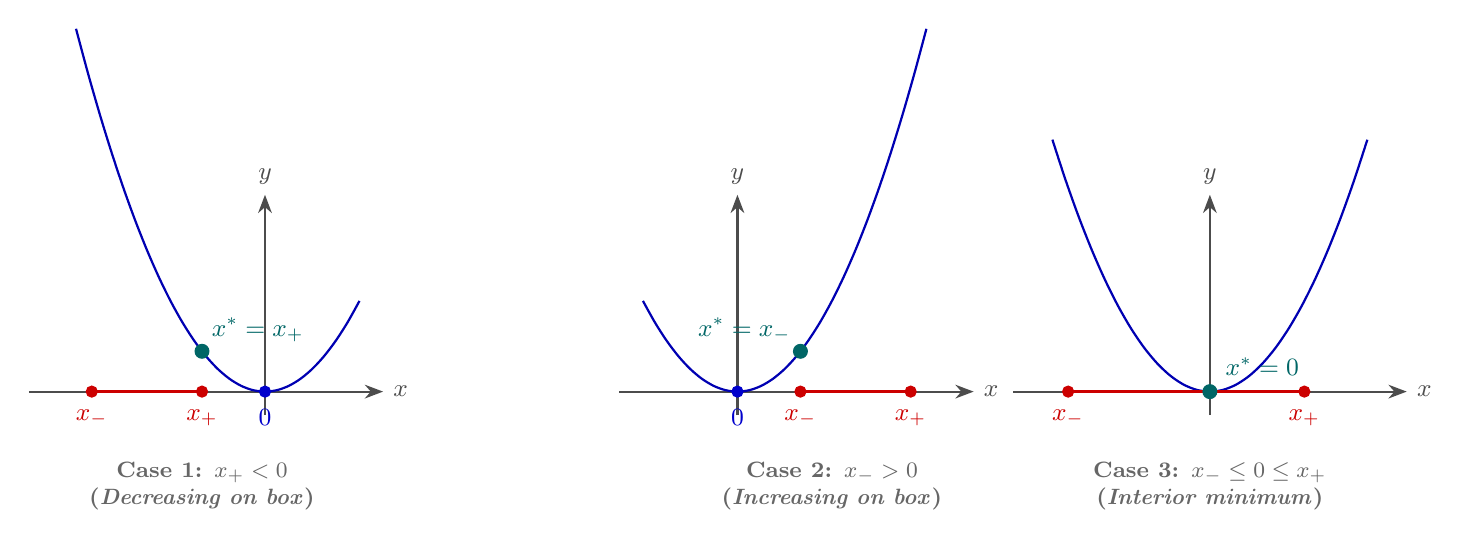
\begin{tikzpicture}[>=Stealth, font=\small]

    % Case 1: Entirely to the left of zero
    \begin{scope}[xshift=-6cm]
        \draw[->, thick, color=gray!60!black] (-3, 0) -- (1.5, 0) node[right] {$x$};
        \draw[->, thick, color=gray!60!black] (0, -0.3) -- (0, 2.5) node[above] {$y$};
        \draw[domain=-2.4:1.2, smooth, variable=\x, blue!70!black, thick] plot ({\x}, {0.8*\x*\x});
        \draw[very thick, red!80!black] (-2.2, 0) -- (-0.8, 0);
        \filldraw[red!80!black] (-2.2, 0) circle (2pt) node[below=3pt] {$x_-$};
        \filldraw[red!80!black] (-0.8, 0) circle (2pt) node[below=3pt] {$x_+$};
        \filldraw[blue!80!black] (0, 0) circle (2pt) node[below=3pt] {$0$};
        \filldraw[teal!80!black] (-0.8, {0.8*(-0.8)*(-0.8)}) circle (2.5pt) node[above right] {$x^* = x_+$};
        \node[align=center, font=\footnotesize\bfseries, color=gray!80!black] at (-0.8, -1.2) {Case 1: $x_+ < 0$\\(\textit{Decreasing on box})};
    \end{scope}

    % Case 2: Entirely to the right of zero
    \begin{scope}[xshift=0cm]
        \draw[->, thick, color=gray!60!black] (-1.5, 0) -- (3, 0) node[right] {$x$};
        \draw[->, thick, color=gray!60!black] (0, -0.3) -- (0, 2.5) node[above] {$y$};
        \draw[domain=-1.2:2.4, smooth, variable=\x, blue!70!black, thick] plot ({\x}, {0.8*\x*\x});
        \draw[very thick, red!80!black] (0.8, 0) -- (2.2, 0);
        \filldraw[blue!80!black] (0, 0) circle (2pt) node[below=3pt] {$0$};
        \filldraw[red!80!black] (0.8, 0) circle (2pt) node[below=3pt] {$x_-$};
        \filldraw[red!80!black] (2.2, 0) circle (2pt) node[below=3pt] {$x_+$};
        \filldraw[teal!80!black] (0.8, {0.8*(0.8)*(0.8)}) circle (2.5pt) node[above left] {$x^* = x_-$};
        \node[align=center, font=\footnotesize\bfseries, color=gray!80!black] at (1.2, -1.2) {Case 2: $x_- > 0$\\(\textit{Increasing on box})};
    \end{scope}

    % Case 3: Zero is contained in the box
    \begin{scope}[xshift=6cm]
        \draw[->, thick, color=gray!60!black] (-2.5, 0) -- (2.5, 0) node[right] {$x$};
        \draw[->, thick, color=gray!60!black] (0, -0.3) -- (0, 2.5) node[above] {$y$};
        \draw[domain=-2.0:2.0, smooth, variable=\x, blue!70!black, thick] plot ({\x}, {0.8*\x*\x});
        \draw[very thick, red!80!black] (-1.8, 0) -- (1.2, 0);
        \filldraw[red!80!black] (-1.8, 0) circle (2pt) node[below=3pt] {$x_-$};
        \filldraw[red!80!black] (1.2, 0) circle (2pt) node[below=3pt] {$x_+$};
        \filldraw[teal!80!black] (0, 0) circle (2.5pt) node[above right=3pt] {$x^* = 0$};
        \node[align=center, font=\footnotesize\bfseries, color=gray!80!black] at (0, -1.2) {Case 3: $x_- \le 0 \le x_+$\\(\textit{Interior minimum})};
    \end{scope}

\end{tikzpicture}%
}
\caption{The three topological configurations for box-constrained homogeneous quadratic optimization over $[x_-, x_+]$.}
\label{fig:parabola-cases-box-en}
\end{figure}

\begin{enumerate}
    \item \textbf{Strictly Negative Configuration ($x_+ < 0$):} the entire box lies to the left of the vertex. The convex parabola is strictly decreasing across the box:
    \begin{align}
    x^* &= x_+, \quad f^* = a (x_+)^2 \\
    x^*_{\max} &= x_-, \quad f^*_{\max} = a (x_-)^2
    \end{align}
    \item \textbf{Strictly Positive Configuration ($x_- > 0$):} the entire box lies to the right of the vertex. The objective is strictly increasing:
    \begin{align}
    x^* &= x_-, \quad f^* = a (x_-)^2 \\
    x^*_{\max} &= x_+, \quad f^*_{\max} = a (x_+)^2
    \end{align}
    \item \textbf{Interior Vertex Configuration ($x_- \le 0 \le x_+$):} the vertex is feasible, so the constrained minimum equals the unconstrained global minimum:
    \begin{align}
    x^* &= 0, \quad f^* = 0
    \end{align}
    The maximum is achieved at whichever boundary point lies furthest from the origin:
    \begin{equation}
    x^*_{\max} = \argmax \{ a(x_-)^2, a(x_+)^2 \} = \begin{cases} x_- & \text{if } |x_-| > |x_+| \\ x_+ & \text{if } |x_+| > |x_-| \end{cases}
    \end{equation}
\end{enumerate}


\FloatBarrier
\section[Univariate Optimization: Non-Homogeneous Quadratic Case]{Univariate Optimization:\\ The Non-Homogeneous Quadratic Case}
\label{sec:opt-non-homogeneous-quadratic}

\subsection{Definition and Non-Separability of the Minimum Operator}
Consider the complete quadratic scalar function with a linear term:
\begin{equation}
f(x) = ax^2 + bx, \quad a, b \in \R, \quad a \neq 0, \; b \neq 0
\end{equation}

\begin{alertblock}{Fundamental Non-Additivity of the Minimum Operator}
In general, minimization does not distribute over sums:
\begin{equation}
\min \{ ax^2 + bx \} \neq \min \{ ax^2 \} + \min \{ bx \}
\end{equation}
The minimum of the sum of two functions does not equal the sum of their individual minima, unless they happen to share the exact same minimizer (which is violated here because the linear term $bx$ has no finite minimum on $\R$).
\end{alertblock}

\subsection{The Coordinate Translation Principle (Origin Shift)}
To solve this problem without relying on differential calculus, we apply one of the most powerful algebraic techniques in optimization: \textbf{coordinate translation}.
We define a shifted variable $z$ around a center $\bar{x} \in \R$ to be determined:
\begin{equation}
z = x - \bar{x} \quad \Longleftrightarrow \quad x = z + \bar{x}
\end{equation}
such that, when expressed in terms of $z$, the quadratic function becomes \textbf{purely homogeneous} (canceling the linear term in $z$).

\subsection{Step-by-Step Algebraic Derivation}
Substituting $x = z + \bar{x}$ into $f(x)$:
\begin{align}
f(z + \bar{x}) &= a(z + \bar{x})^2 + b(z + \bar{x}) \nonumber\\
&= a\left(z^2 + 2z\bar{x} + \bar{x}^2\right) + bz + b\bar{x} \nonumber\\
&= az^2 + 2a\bar{x}z + a\bar{x}^2 + bz + b\bar{x}
\end{align}
Grouping terms by descending powers of $z$:
\begin{equation}
f(z + \bar{x}) = az^2 + (2a\bar{x} + b)z + \left(a\bar{x}^2 + b\bar{x}\right)
\end{equation}
Notice that the constant term independent of $z$ is exactly the value of the original function evaluated at $\bar{x}$:
\begin{equation}
a\bar{x}^2 + b\bar{x} = f(\bar{x})
\end{equation}
Thus the transformed function is written as:
\begin{equation}
f(z + \bar{x}) = az^2 + (2a\bar{x} + b)z + f(\bar{x})
\end{equation}

To eliminate the linear term and render the function homogeneous in $z$, we set the coefficient of $z$ to zero:
\begin{equation}
2a\bar{x} + b = 0 \quad \Longrightarrow \quad \bar{x} = -\frac{b}{2a}
\end{equation}

\subsection{Solution in Shifted Coordinates and Inverse Mapping}
Setting $\bar{x} = -\frac{b}{2a}$, the function in $z$ becomes decoupled:
\begin{equation}
g(z) = f(z + \bar{x}) = az^2 + f(\bar{x})
\end{equation}
Since $f(\bar{x})$ is an additive constant independent of the optimization variable $z$:
\begin{equation}
\argmin_{z \in \R} g(z) = \argmin_{z \in \R} \left( az^2 + f(\bar{x}) \right) = \argmin_{z \in \R} \left( az^2 \right)
\end{equation}

For $a > 0$ (convex parabola), the minimizer in shifted space is immediate:
\begin{equation}
z^* = 0
\end{equation}
Mapping back to the original coordinate space:
\begin{equation}
x^* = z^* + \bar{x} = 0 + \bar{x} = -\frac{b}{2a}
\end{equation}
The optimal value is found by evaluating $f$ at $x^* = \bar{x}$:
\begin{align}
f^* = f(\bar{x}) &= a\left(-\frac{b}{2a}\right)^2 + b\left(-\frac{b}{2a}\right) \nonumber\\
&= a\frac{b^2}{4a^2} - \frac{b^2}{2a} = \frac{b^2}{4a} - \frac{2b^2}{4a} = -\frac{b^2}{4a}
\end{align}

\begin{figure}[H]
\centering
\resizebox{0.88\textwidth}{!}{%
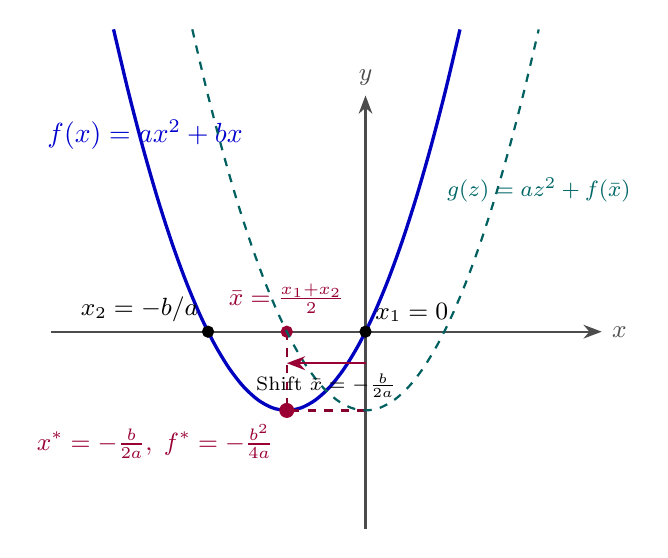
\begin{tikzpicture}[>=Stealth, font=\small]

    % Coordinate axes
    \draw[->, thick, color=gray!60!black] (-4, 0) -- (3, 0) node[right] {$x$};
    \draw[->, thick, color=gray!60!black] (0, -2.5) -- (0, 3) node[above] {$y$};

    % Original parabola f(x) = x^2 + 2x = x(x+2), roots 0 and -2, vertex (-1, -1)
    \draw[domain=-3.2:1.2, smooth, variable=\x, blue!75!black, very thick] plot ({\x}, {\x*\x + 2*\x});
    \node[blue!80!black, font=\bfseries] at (-2.8, 2.5) {$f(x) = ax^2 + bx$};

    % Roots
    \filldraw[black] (0, 0) circle (2pt) node[above right] {$x_1 = 0$};
    \filldraw[black] (-2, 0) circle (2pt) node[above left] {$x_2 = -b/a$};

    % Vertex and midpoint
    \draw[dashed, color=purple!70!black, thick] (-1, 0) -- (-1, -1) -- (0, -1);
    \filldraw[purple!80!black] (-1, -1) circle (2.5pt) node[below left=2pt] {$x^* = -\frac{b}{2a}, \; f^* = -\frac{b^2}{4a}$};
    \filldraw[purple!80!black] (-1, 0) circle (2pt) node[above=3pt] {$\bar{x} = \frac{x_1 + x_2}{2}$};

    % Shifted homogeneous parabola g(z) = z^2 - 1
    \draw[domain=-2.2:2.2, smooth, variable=\z, teal!75!black, thick, dashed] plot ({\z}, {\z*\z - 1});
    \node[teal!80!black, font=\footnotesize] at (2.2, 1.8) {$g(z) = az^2 + f(\bar{x})$};

    % Shift arrow
    \draw[->, thick, draw=purple!80!black] (0, -0.4) -- (-1, -0.4) node[midway, below, font=\scriptsize] {Shift $\bar{x} = -\frac{b}{2a}$};

\end{tikzpicture}%
}
\caption{Geometric visualization of coordinate translation for the non-homogeneous parabola: the vertex $x^*$ lies precisely at the midpoint between the two roots $x_1$ and $x_2$.}
\label{fig:coordinate-shift-parabola-en}
\end{figure}

\subsection{Geometric Interpretation: The Midpoint of the Roots}
The quadratic function $f(x) = ax^2 + bx = x(ax + b)$ always possesses two real roots (when $b \neq 0$):
\begin{equation}
x_1 = 0, \quad x_2 = -\frac{b}{a}
\end{equation}
The optimal minimizer derived via coordinate shift lies exactly at the \textbf{midpoint} of the roots:
\begin{equation}
\bar{x} = \frac{x_1 + x_2}{2} = \frac{0 + (-b/a)}{2} = -\frac{b}{2a}
\end{equation}
This universal symmetry property reflects the fact that the derivative of a degree-two polynomial is an affine line intersecting the horizontal axis at the exact arithmetic mean of its real zeros.

\subsection[Box-Constrained General Quadratic Optimization]{Box-Constrained Optimization\\ for General Quadratic Functions}
Under a box constraint $x \in [x_-, x_+]$, coordinate translation directly shifts the boundary endpoints for variable $z$:
\begin{equation}
x \in [x_-, x_+] \quad \Longleftrightarrow \quad z \in [x_- - \bar{x}, \; x_+ - \bar{x}]
\end{equation}
Setting $z_- = x_- - \bar{x}$ and $z_+ = x_+ - \bar{x}$, the problem reduces to the homogeneous quadratic problem over $[z_-, z_+]$ solved in Section~\ref{sec:opt-homogeneous-quadratic}:
\begin{equation}
z^* = \begin{cases}
z_+ & \text{if } z_+ < 0 \\
z_- & \text{if } z_- > 0 \\
0 & \text{if } z_- \le 0 \le z_+
\end{cases}
\end{equation}
recovering the original variable solution via $x^* = z^* + \bar{x}$.


\FloatBarrier
\section{Synoptic Formula Reference of Univariate Optimization}
\label{sec:opt-synoptic-reference}

\begin{table}[H]
\centering
\small
\renewcommand{\arraystretch}{1.3}
\begin{tabularx}{\textwidth}{l c l X c}
\toprule
\textbf{Class} & \textbf{Form} & \textbf{Condition} & \textbf{Minimum $x^*$} & \textbf{Value $f^*$} \\
\midrule
\textbf{Linear} & $bx$ & $b > 0$ & Does not exist ($x \to -\infty$) & $-\infty$ \\
                &      & $b < 0$ & Does not exist ($x \to +\infty$) & $-\infty$ \\
                &      & $b = 0$ (degenerate) & Indifferent ($\forall x \in \R$) & $0$ \\
\midrule
\textbf{Homogeneous} & $ax^2$ & $a > 0$ (convex) & $x^* = 0$ (unique) & $0$ \\
\textbf{quadratic}   &        & $a < 0$ (concave) & Does not exist ($x \to \pm\infty$) & $-\infty$ \\
                     &        & $a = 0$ (degenerate) & Indifferent ($\forall x \in \R$) & $0$ \\
\midrule
\textbf{General}   & $ax^2 + bx$ & $a > 0$ (convex) & $x^* = -b/(2a)$ (vertex) & $-b^2/(4a)$ \\
\textbf{quadratic} &             & $a < 0$ (concave) & Does not exist ($x \to \pm\infty$) & $-\infty$ \\
                   &             & $a = 0, \; b \neq 0$ & Does not exist (linear reduction) & $-\infty$ \\
\bottomrule
\end{tabularx}
\caption{Comprehensive synoptic summary of univariate unconstrained optimization.}
\label{tab:synoptic-univariate-en}
\end{table}

\chapter{Multivariate Optimization: Geometry, Linear Functions, and Quadratic Forms}
\label{chap:opt-multivariate-linear-quadratic}

\section{From Univariate to Multivariate: Dimensionality of \texorpdfstring{$\R^n$}{R\textasciicircum n}}
\label{sec:opt-dimensionality-rn-en}

\subsection{Multivariate Input Space}
In modern data science, machine learning, and computational engineering, models almost universally depend on a collection of mutually interacting variables. The primary mathematical object of study is the real-valued multivariate scalar function:
\begin{equation}
f: \R^n \to \R, \quad f(x) = f(x_1, x_2, \dots, x_n)
\end{equation}
where the input argument $x$ is a structured column vector of $n$ real numbers:
\begin{equation}
x = \begin{bmatrix} x_1 \\ x_2 \\ \vdots \\ x_n \end{bmatrix} = [x_i]_{i=1}^n \in \R^n
\end{equation}

Vector dimension $n$ spans radically disparate orders of magnitude across application domains:
\begin{itemize}
    \item \textbf{Small scale ($n \in \{2, 3, 10^2\}$):} Euclidean geometric models, inverse kinematics, elementary resource allocation.
    \item \textbf{Medium and large scale ($n \in \{10^4, 10^5\}$):} image and signal processing, finite element structural mechanics, network flow logistics.
    \item \textbf{Monstrous scale (\textit{heinously large}, $n \in \{10^9, 10^{11}\}$):} training deep neural networks and Large Language Models (LLMs), where $n$ enumerates synaptic weights and attention matrices.
\end{itemize}

\subsection{The Curse of Dimensionality}
The continuous vector space $\R^n$ is formally defined as the Cartesian product of $\R$ taken $n$ times:
\begin{equation}
\R^n = \underbrace{\R \times \R \times \dots \times \R}_{n \text{ times}}
\end{equation}

\begin{noteblock}{Exponential Volumetric Expansion}
The volume of available space within $\R^n$ grows exponentially with dimension $n$. Adding variables to an optimization model is never computationally neutral: it fundamentally changes the geometric density of the searchable space.
\end{noteblock}

To quantitatively demonstrate this combinatorial explosion, consider a drastic simplification:
\begin{enumerate}
    \item Restrict the continuous domain to a compact unit hypercube (\textit{box}):
    \begin{equation}
    X = \{x \in \R^n : 0 \le x_i \le 1, \; i = 1, \dots, n\} = [0, 1]^n
    \end{equation}
    \item Discard interior continuity entirely, sampling only the extreme discrete corner values for each coordinate, $x_i \in \{0, 1\}$.
\end{enumerate}

The resulting set coincides with the vertices of the \textbf{Boolean hypercube} $\{0, 1\}^n$, whose cardinality is:
\begin{equation}
|V| = 2^n \text{ vertices}
\end{equation}
Even for modest dimensions (such as $n = 100$), $2^{100} \approx 1.26 \times 10^{30}$. This number dwarfs the processing capacity of all existing computing clusters, rendering brute-force grid enumeration information-theoretically impossible.


\FloatBarrier
\section{Vector and Multi-Objective Optimization}
\label{sec:opt-vector-multiobjective-en}

\subsection{The Limitation of a Single Scalar Objective}
Standard optimization assumes that the overall merit of any decision $x \in X$ can be collapsed into a single real number $f(x) \in \R$. 

Because the real line $\R$ is endowed with a \textbf{total order}:
\begin{equation}
\forall a, b \in \R \implies a \le b \quad \lor \quad b \le a
\end{equation}
any two candidate solutions $x'$ and $x''$ can always be unambiguously ranked by comparing $f(x')$ with $f(x'')$.

In practice, complex decision problems require balancing multiple competing, incommensurable criteria (comparing ``apples to oranges''):
\begin{itemize}
    \item \textbf{Vehicle procurement:} capital cost vs fuel economy vs safety ratings vs styling appeal.
    \item \textbf{Machine learning:} minimizing empirical data loss $\mathcal{L}(w)$ vs minimizing model complexity $R(w)$ to prevent overfitting.
\end{itemize}

A formal \textbf{multi-objective} (or vector) optimization problem is posed as:
\begin{equation}
\min_{x \in X} F(x) = \begin{bmatrix} f_1(x) \\ f_2(x) \\ \vdots \\ f_k(x) \end{bmatrix}, \quad F: X \to \R^k, \; k \ge 2
\end{equation}

\subsection{Illustrative Example: Markowitz Portfolio Selection}
Consider an investor distributing capital across a set of financial assets:
\begin{itemize}
    \item \textbf{Objective 1 (Expected Return):} $f_1(x) \in \R$, to be maximized (or $-f_1(x)$ minimized).
    \item \textbf{Objective 2 (Financial Risk / Volatility):} $f_2(x) \in \R$ (return variance), to be minimized.
\end{itemize}
Safe assets (e.g., short-term government bonds) deliver low returns, whereas high-yield equities carry significant volatility. No single portfolio simultaneously minimizes variance and maximizes return.

\subsection{Partial Ordering and the Pareto Frontier}
For $k \ge 2$, vector space $\R^k$ lacks a natural total ordering. Instead, it is governed by a \textbf{partial ordering} induced by the non-negative orthant cone:
\begin{equation}
u \le v \iff u_i \le v_i \quad \forall i = 1, \dots, k
\end{equation}

\begin{definition}[Pareto Dominance]
Assuming by convention that all $k$ objectives are to be minimized, a feasible point $x' \in X$ \textbf{Pareto-dominates} $x'' \in X$ (denoted $x' \succ_P x''$) if and only if:
\begin{equation}
f_i(x') \le f_i(x'') \quad \forall i \in \{1, \dots, k\} \quad \land \quad \exists j \in \{1, \dots, k\} : f_j(x') < f_j(x'')
\end{equation}
\end{definition}

\begin{definition}[Non-Dominated or Pareto-Optimal Solution]
A point $x^* \in X$ is \textbf{Pareto-optimal} (or non-dominated) if no other point $x \in X$ dominates $x^*$. The collection of all objective values $F(x^*)$ forms the \textbf{Pareto Frontier}.
\end{definition}

\begin{figure}[H]
\centering
\resizebox{0.92\textwidth}{!}{%
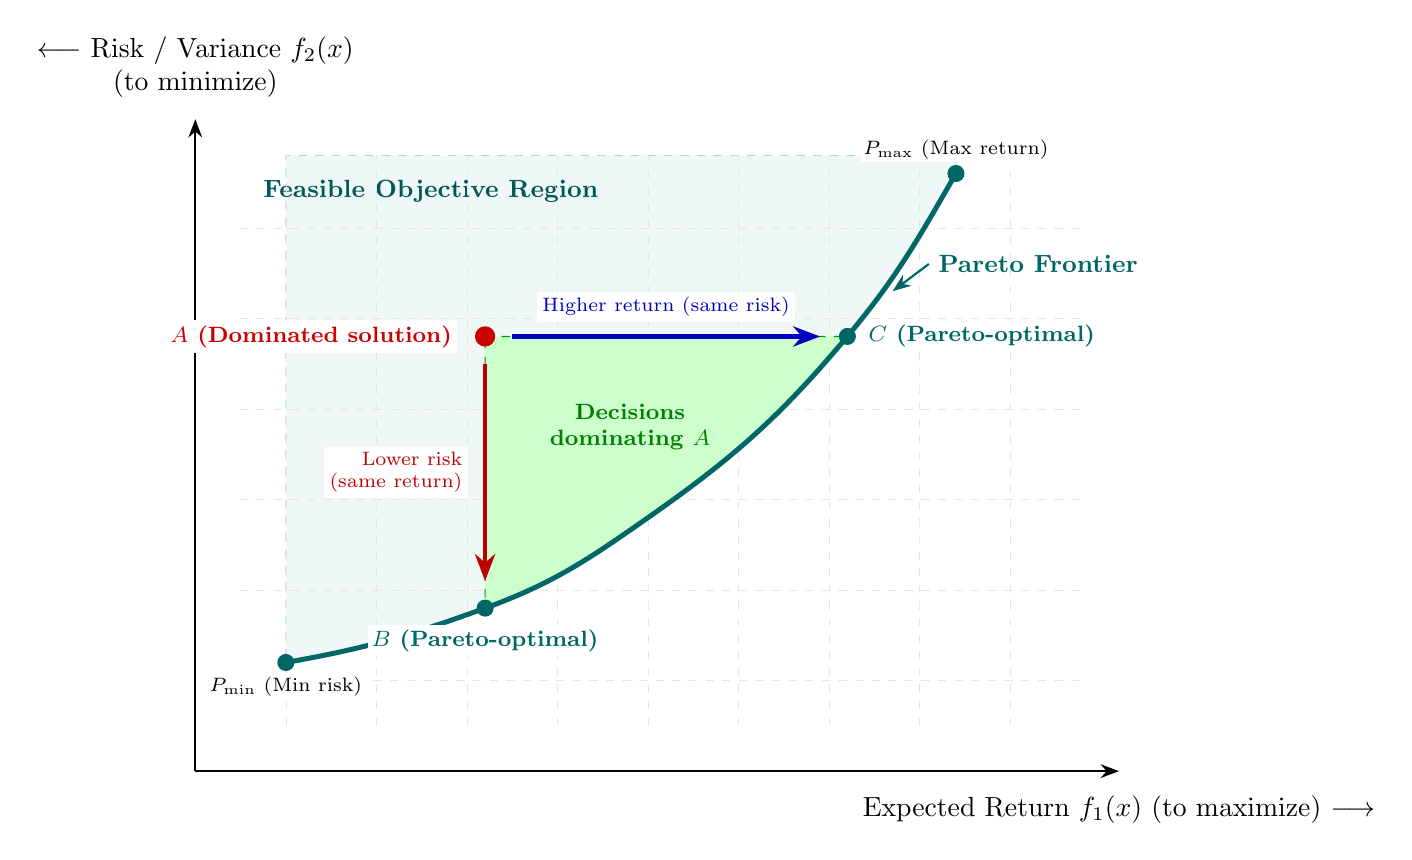
\begin{tikzpicture}[>=Stealth, scale=1.15]
    % Background Feasible Area
    \fill[teal!6, draw=teal!30, dashed, thin]
        (1.0, 1.2) 
        to[out=10, in=200] (3.2, 1.8) 
        to[out=20, in=215] (5.0, 2.8) 
        to[out=35, in=230] (7.2, 4.8) 
        to[out=50, in=240] (8.4, 6.6)
        -- (8.4, 6.8) -- (1.0, 6.8) -- cycle;
    \node[teal!70!black, font=\small\bfseries] at (2.6, 6.4) {Feasible Objective Region};

    % Axes
    \draw[->, thick] (0,0) -- (10.2,0) node[below=5pt] {Expected Return $f_1(x)$ (to maximize) $\longrightarrow$};
    \draw[->, thick] (0,0) -- (0,7.2) node[above=4pt, align=center] {$\longleftarrow$ Risk / Variance $f_2(x)$\\(to minimize)};
    \draw[help lines, color=gray!20, dashed] (0.5,0.5) grid (9.8,6.8);

    % Dominance region from A (feasible points dominating A)
    \fill[green!20, draw=green!60!black, dashed, thin] 
        (3.2, 4.8) -- (7.2, 4.8) 
        to[out=230, in=35] (5.0, 2.8) 
        to[out=215, in=20] (3.2, 1.8) -- cycle;
    \node[green!50!black, font=\footnotesize\bfseries, align=center] at (4.8, 3.8) {Decisions\\dominating $A$};

    % Pareto Frontier Curve (Convex lower boundary)
    \draw[line width=1.8pt, teal!80!black] 
        (1.0, 1.2) 
        to[out=10, in=200] (3.2, 1.8) 
        to[out=20, in=215] (5.0, 2.8) 
        to[out=35, in=230] (7.2, 4.8) 
        to[out=50, in=240] (8.4, 6.6);

    % Frontier Title Callout (in upper right section)
    \node[teal!80!black, font=\small\bfseries, anchor=west] (pareto_label) at (8.1, 5.6) {Pareto Frontier};
    \draw[->, thick, teal!80!black] (pareto_label.west) -- (7.7, 5.3);

    % Frontier Extreme Points
    \filldraw[teal!80!black] (1.0, 1.2) circle (2.5pt);
    \node[below=4pt, font=\scriptsize, fill=white, inner sep=1pt] at (1.0, 1.2) {$P_{\text{min}}$ (Min risk)};

    \filldraw[teal!80!black] (8.4, 6.6) circle (2.5pt);
    \node[above=4pt, font=\scriptsize, fill=white, inner sep=1pt] at (8.4, 6.6) {$P_{\text{max}}$ (Max return)};

    % Frontier Comparison Points B and C
    \coordinate (B) at (3.2, 1.8);
    \coordinate (C) at (7.2, 4.8);

    \filldraw[teal!80!black] (B) circle (2.5pt);
    \node[below=6pt, font=\footnotesize\bfseries, teal!80!black, fill=white, inner sep=1.5pt] at (B) {$B$ (Pareto-optimal)};

    \filldraw[teal!80!black] (C) circle (2.5pt);
    \node[right=6pt, font=\footnotesize\bfseries, teal!80!black, fill=white, inner sep=1.5pt] at (C) {$C$ (Pareto-optimal)};

    % Dominated point A
    \coordinate (A) at (3.2, 4.8);
    \filldraw[red!80!black] (A) circle (3pt);
    \node[anchor=east, font=\footnotesize\bfseries, red!80!black, fill=white, inner sep=2pt] at (2.9, 4.8) {$A$ (Dominated solution)};

    % Comparison arrows from A
    % 1. Downward to B (same return, lower risk)
    \draw[->, >=Stealth, line width=1.5pt, red!75!black] (3.2, 4.5) -- (3.2, 2.1);
    \node[left=6pt, font=\scriptsize, red!75!black, align=right, fill=white, inner sep=2pt] at (3.2, 3.3) {Lower risk\\(same return)};

    % 2. Rightward to C (same risk, higher return)
    \draw[->, >=Stealth, line width=1.5pt, blue!75!black] (3.5, 4.8) -- (6.9, 4.8);
    \node[above=5pt, font=\scriptsize, blue!75!black, fill=white, inner sep=2pt] at (5.2, 4.8) {Higher return (same risk)};
\end{tikzpicture}%
}
\caption{Geometric representation of the Pareto Frontier in Markowitz portfolio selection.}
\label{fig:pareto-frontier-en}
\end{figure}

An optimization algorithm cannot objectively choose a single point on the Pareto frontier: the final selection rests with human decision-makers and their risk preferences.

\subsection{Operational Reduction Techniques: Scalarization and Budgeting}
To apply continuous optimization solvers to multi-objective problems, two strategies are standard:
\begin{enumerate}
    \item \textbf{Scalarization:} Formulate a weighted linear or convex combination of objectives:
    \begin{equation}
    \min_{x \in X} \left\{ f_1(x) + \alpha f_2(x) \right\}, \quad \alpha > 0
    \end{equation}
    Here $\alpha$ serves as an \textit{exchange rate}: how much degradation in $f_1$ is tolerated to gain one unit of improvement in $f_2$. Sweeping $\alpha \in (0, +\infty)$ traces the Pareto frontier. In machine learning, regularized empirical risk minimization:
    \begin{equation}
    \min_w \left\{ \mathcal{L}(w) + \lambda R(w) \right\}
    \end{equation}
    is a classic scalarization, where trade-off parameter $\lambda$ is selected via cross-validation.
    
    \item \textbf{Constraint Method (\textit{Budgeting}):} Designate a primary objective to optimize, downgrading all other criteria to upper/lower bound constraints (budgets):
    \begin{equation}
    \min_{x \in X} \{ f_1(x) : f_2(x) \le \beta_2, \; \dots, \; f_k(x) \le \beta_k \}
    \end{equation}
    Systematically varying the budget vector $\beta$ traces the non-dominated set.
\end{enumerate}

\begin{noteblock}{Standard Convention}
Unless stated otherwise, modeling is assumed to have already consolidated the problem into a single scalar objective $f: \R^n \to \R$.
\end{noteblock}


\FloatBarrier
\section{Euclidean Geometry in \texorpdfstring{$\R^n$}{R\textasciicircum n} and Function Tomography}
\label{sec:opt-euclidean-geometry-tomography-en}

\subsection{Standard Inner Product and Induced Norm}
For any two vectors $x, z \in \R^n$, the \textbf{standard Euclidean inner product} is:
\begin{equation}
\langle x, z \rangle = x^T z = \sum_{i=1}^n x_i z_i = x_1 z_1 + x_2 z_2 + \dots + x_n z_n
\end{equation}
The inner product satisfies symmetry ($\langle x, z \rangle = \langle z, x \rangle$), bilinearity, and positive definiteness ($\langle x, x \rangle > 0$ for all $x \neq 0$).

The \textbf{Euclidean norm} ($\ell_2$-norm) measures geometric length:
\begin{equation}
\|x\| = \sqrt{\langle x, x \rangle} = \sqrt{\sum_{i=1}^n x_i^2}
\end{equation}

\subsection{Angular Representation and the Cauchy-Schwarz Inequality}
Geometrically, the inner product relates lengths to the angle $\theta \in [0, \pi]$ between $x$ and $z$:
\begin{equation}
\langle x, z \rangle = \|x\| \|z\| \cos(\theta)
\end{equation}
yielding three geometric orientations:
\begin{itemize}
    \item $\langle x, z \rangle > 0 \iff \theta \in [0, \pi/2)$: acute angle (pointing in the same general direction).
    \item $\langle x, z \rangle = 0 \iff \theta = \pi/2$: \textbf{orthogonal} vectors ($x \perp z$).
    \item $\langle x, z \rangle < 0 \iff \theta \in (\pi/2, \pi]$: obtuse angle (pointing in opposing directions).
\end{itemize}

Since $|\cos(\theta)| \le 1$, the fundamental \textbf{Cauchy-Schwarz inequality} follows directly:
\begin{equation}
|\langle x, z \rangle| \le \|x\| \|z\|, \quad \forall x, z \in \R^n
\end{equation}
with equality holding if and only if $x$ and $z$ are collinear ($x = \gamma z$ for some $\gamma \in \R$).

\subsection{The Concept of Function Tomography}
In multivariate space ($n \ge 3$), the graph $\text{gr}(f) = \{(x, f(x)) : x \in \R^n\} \subset \R^{n+1}$ cannot be visualized. The central analytical tool used to investigate its local and global behavior is \textbf{tomography}.

\begin{definition}[Directional Tomography]
Given a base point $x \in \R^n$ and a non-zero directional vector $d \in \R^n \setminus \{0\}$, the \textbf{tomography} of $f$ from $x$ along direction $d$ is the univariate function $\phi_{x, d}: \R \to \R$:
\begin{equation}
\phi_{x, d}(\alpha) = f(x + \alpha d), \quad \alpha \in \R
\end{equation}
\end{definition}

Scalar $\alpha$ represents the signed displacement step along the line through $x$ oriented by $d$.

Directional norm $\|d\|$ simply scales the parameter $\alpha$:
\begin{equation}
\phi_{x, \beta d}(\alpha) = f(x + \alpha (\beta d)) = \phi_{x, d}(\alpha \beta)
\end{equation}
To eliminate scaling ambiguity, it is standard practice to normalize the search direction:
\begin{equation}
\|d\| = 1
\end{equation}


\FloatBarrier
\section{Multivariate Linear Functions}
\label{sec:opt-multivariate-linear-functions-en}

\subsection{Definition and Separability}
A multivariate function $f: \R^n \to \R$ is \textbf{linear} if it can be represented as an inner product with a fixed coefficient vector $b \in \R^n$:
\begin{equation}
f(x) = \langle b, x \rangle = b^T x = \sum_{i=1}^n b_i x_i
\end{equation}

Every multivariate linear function is inherently \textbf{separable}: it is the sum of $n$ independent univariate linear functions:
\begin{equation}
f(x) = \sum_{i=1}^n f_i(x_i), \quad \text{with } f_i(x_i) = b_i x_i
\end{equation}
There are no bilinear cross-terms between different variables.

\subsection{Geometry of Graph and Level Sets}
\begin{itemize}
    \item \textbf{Graph:} $\text{gr}(f) = \{(x, b^T x) : x \in \R^n\}$ is an $n$-dimensional hyperplane in $\R^{n+1}$ passing through the origin.
    \item \textbf{Level Sets:} For any target value $v \in \R$, the level set is:
    \begin{equation}
    L(f, v) = \{x \in \R^n : b^T x = v\}
    \end{equation}
    This set forms an $(n-1)$-dimensional affine hyperplane in $\R^n$. As $v$ varies, level sets form an infinite family of parallel hyperplanes.
\end{itemize}

\begin{theorem}[Orthogonality of Vector $b$ to Level Sets]
The coefficient vector $b$ is strictly orthogonal to any tangent direction within the level sets $L(f, v)$, for all $v \in \R$.
\end{theorem}

\begin{proof}
Let $x, z \in L(f, v)$ be two arbitrary points on the same level set. By definition:
\begin{equation}
b^T x = v \quad \land \quad b^T z = v
\end{equation}
Subtracting these expressions yields:
\begin{equation}
b^T z - b^T x = 0 \iff b^T (z - x) = 0 \iff \langle b, z - x \rangle = 0
\end{equation}
Vector $z - x$ represents an arbitrary displacement tangent to the level hyperplane. Because $b$ is orthogonal to every displacement within the level set, $b \perp L(f, v)$.
\end{proof}


\FloatBarrier
\section{Linear Tomography and Steepest Descent Direction}
\label{sec:opt-linear-tomography-steepest-descent-en}

\subsection{Tomographic Cross-Section Computation}
Fixing the origin $x = 0$ and a unit direction $\|d\| = 1$, the tomography of linear function $f(x) = b^T x$ is:
\begin{equation}
\phi_{0, d}(\alpha) = f(0 + \alpha d) = b^T (\alpha d) = \alpha \langle b, d \rangle = \alpha \|b\| \|d\| \cos(\theta) = \alpha \|b\| \cos(\theta)
\end{equation}
where $\theta$ is the angle between coefficient vector $b$ and direction $d$.

The tomography is a \textbf{univariate line} through the origin whose slope is governed by $\langle b, d \rangle$.

\subsection{Directional Analysis: The Radar Screen Analogy}
Rotating direction $d$ through all angles reveals five fundamental behaviors:
\begin{enumerate}
    \item \textbf{$d$ perfectly aligned with $b$ ($\theta = 0 \implies \cos(\theta) = 1$):}
    \begin{equation}
    \phi_{0, d}(\alpha) = \alpha \|b\|
    \end{equation}
    The line exhibits maximum positive slope: the function increases at the highest possible rate (\textbf{steepest ascent}).
    
    \item \textbf{$d$ acute to $b$ ($\theta \in (0, \pi/2) \implies \cos(\theta) > 0$):}
    Positive slope, strictly bounded above by $\|b\|$.
    
    \item \textbf{$d$ orthogonal to $b$ ($\theta = \pi/2 \implies \cos(\theta) = 0$):}
    \begin{equation}
    \phi_{0, d}(\alpha) = 0, \quad \forall \alpha \in \R
    \end{equation}
    The tomography is identically flat. Moving orthogonally to $b$ corresponds to walking along the level set $L(f, 0)$, leaving the objective value unchanged.
    
    \item \textbf{$d$ obtuse to $b$ ($\theta \in (\pi/2, \pi) \implies \cos(\theta) < 0$):}
    Negative slope: advancing along positive $\alpha$ decreases the function.
    
    \item \textbf{$d$ opposite to $b$ ($\theta = \pi \implies \cos(\theta) = -1$):}
    \begin{equation}
    \phi_{0, d}(\alpha) = -\alpha \|b\|
    \end{equation}
    The line achieves the steepest negative slope (\textbf{steepest descent}).
\end{enumerate}

\begin{figure}[H]
\centering
\resizebox{0.90\textwidth}{!}{%
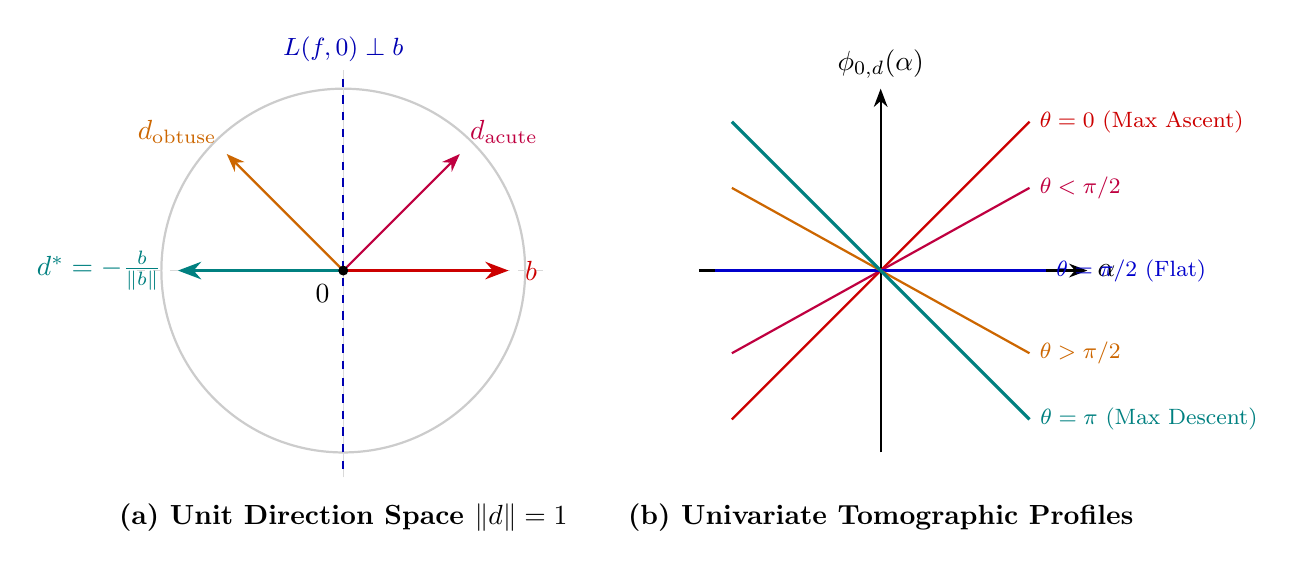
\begin{tikzpicture}[>=Stealth, scale=1.05]
    % Left panel: Radar circle
    \draw[thick, gray!40] (0,0) circle (2.2cm);
    \draw[help lines, color=gray!30, dashed] (-2.5,0) -- (2.5,0);
    \draw[help lines, color=gray!30, dashed] (0,-2.5) -- (0,2.5);

    % Level set line (orthogonal to b)
    \draw[thick, dashed, blue!70!black] (0,-2.4) -- (0,2.4) node[above, font=\small] {$L(f, 0) \perp b$};

    % Vector b
    \draw[->, very thick, red!80!black] (0,0) -- (2.0,0) node[right=2pt] {$b$};

    % Direction d1 (steepest descent)
    \draw[->, very thick, teal] (0,0) -- (-2.0,0) node[left=2pt] {$d^* = -\frac{b}{\|b\|}$};

    % Direction d2 (steepest ascent)
    \draw[->, thick, purple] (0,0) -- (1.41, 1.41) node[above right] {$d_{\text{acute}}$};
    \draw[->, thick, orange!80!black] (0,0) -- (-1.41, 1.41) node[above left] {$d_{\text{obtuse}}$};

    % Center
    \filldraw (0,0) circle (1.5pt) node[below left=2pt] {$0$};
    \node[below] at (0,-2.7) {\textbf{(a) Unit Direction Space $\|d\|=1$}};

    % Right panel: Tomography profiles
    \begin{scope}[shift={(6.5, 0)}]
        \draw[->, thick] (-2.2,0) -- (2.5,0) node[right] {$\alpha$};
        \draw[->, thick] (0,-2.2) -- (0,2.2) node[above] {$\phi_{0, d}(\alpha)$};

        % Max ascent
        \draw[thick, red!80!black] (-1.8,-1.8) -- (1.8,1.8) node[right, font=\footnotesize] {$\theta = 0$ (Max Ascent)};
        % Moderate ascent
        \draw[thick, purple] (-1.8,-1.0) -- (1.8,1.0) node[right, font=\footnotesize] {$\theta < \pi/2$};
        % Flat
        \draw[thick, blue!80!black] (-2.0,0) -- (2.0,0) node[right, font=\footnotesize] {$\theta = \pi/2$ (Flat)};
        % Moderate descent
        \draw[thick, orange!80!black] (-1.8,1.0) -- (1.8,-1.0) node[right, font=\footnotesize] {$\theta > \pi/2$};
        % Max descent
        \draw[very thick, teal] (-1.8,1.8) -- (1.8,-1.8) node[right, font=\footnotesize] {$\theta = \pi$ (Max Descent)};

        \node[below] at (0,-2.7) {\textbf{(b) Univariate Tomographic Profiles}};
    \end{scope}
\end{tikzpicture}%
}
\caption{Tomographic inspection of a linear function: rotating search directions and identifying slope bounds.}
\label{fig:linear-tomography-en}
\end{figure}

\subsection{Formal Derivation of the Steepest Descent Direction}
Suppose an algorithm stands at the origin and takes a single step of fixed length $\|\Delta x\| = \varepsilon > 0$. The resulting change in objective value is:
\begin{equation}
\Delta f = f(\varepsilon d) - f(0) = \varepsilon \langle b, d \rangle = \varepsilon \|b\| \cos(\theta)
\end{equation}
To achieve maximal reduction ($\Delta f < 0$ minimized), with $\varepsilon > 0$ and $\|d\| = 1$, one solves:
\begin{equation}
\min_{\|d\| = 1} \langle b, d \rangle = \min_{\|d\|=1} \|b\| \cos(\theta)
\end{equation}
Cosine reaches its absolute minimum $-1$ uniquely at $\theta = \pi$, producing the canonical result:
\begin{equation}
d^* = -\frac{b}{\|b\|}
\end{equation}

\begin{noteblock}{Antigradient Principle}
The direction yielding the greatest instantaneous rate of decrease for a linear objective is strictly the \textbf{antigradient} $-b$.
\end{noteblock}


\FloatBarrier
\section{From Linear to Quadratic Functions: The Separable Case}
\label{sec:opt-separable-quadratic-en}

\subsection{Separable Quadratic Functions}
The most direct extension of univariate quadratic functions to $n$ dimensions sums $n$ independent scalar parabolas:
\begin{equation}
f(x) = \sum_{i=1}^n \left( a_i x_i^2 + b_i x_i \right), \quad a, b \in \R^n
\end{equation}

When $a_i = 1$ and $b_i = 0$ for all $i$, the function is the squared Euclidean norm:
\begin{equation}
f(x) = \sum_{i=1}^n x_i^2 = \|x\|^2
\end{equation}
Its level sets $L(f, v) = \{x \in \R^n : \|x\|^2 = v\}$ are concentric hyperspheres of radius $r = \sqrt{v}$.

\subsection{Anisotropic Curvature and Eccentricity}
In dimension $n = 2$, setting $b = 0$, $a_2 = 1$ and varying parameter $a_1 = a > 0$:
\begin{equation}
f(x_1, x_2) = a x_1^2 + x_2^2
\end{equation}
Level sets for a positive value $v > 0$ satisfy:
\begin{equation}
a x_1^2 + x_2^2 = v \iff \frac{x_1^2}{v/a} + \frac{x_2^2}{v} = 1
\end{equation}
The geometry depends directly on the curvature ratio:
\begin{itemize}
    \item \textbf{If $a = 1$:} equal semi-axes ($\sqrt{v/a} = \sqrt{v}$): the level set is a circle.
    \item \textbf{If $a > 1$:} curvature is higher along $x_1$. Level curves reach $v$ closer to the origin along $x_1$ ($|x_1| = \sqrt{v/a} < \sqrt{v}$): the ellipse is \textbf{vertically elongated}.
    \item \textbf{If $0 < a < 1$:} curvature along $x_1$ is gentler: the ellipse is \textbf{horizontally elongated}.
    \item \textbf{As $a \to 0^+$:} horizontal curvature vanishes; semi-axis $\sqrt{v/a} \to +\infty$: the ellipse degenerates into two parallel lines $x_2 = \pm \sqrt{v}$.
\end{itemize}


\FloatBarrier
\section{General Homogeneous Quadratic Forms and Symmetrization}
\label{sec:opt-general-quadratic-symmetrization-en}

\subsection{Definition and Cross-Terms}
General homogeneous quadratic functions contain bilinear cross-terms $x_i x_j$ with $i \neq j$:
\begin{equation}
f(x) = \frac{1}{2} x^T Q x = \frac{1}{2} \sum_{i=1}^n \sum_{j=1}^n Q_{ij} x_i x_j = \frac{1}{2} \sum_{i=1}^n Q_{ii} x_i^2 + \frac{1}{2} \sum_{i=1}^n \sum_{j \neq i} Q_{ij} x_i x_j
\end{equation}
where $Q \in \R^{n \times n}$ is a given square matrix. The $1/2$ prefactor ensures the Hessian matrix equals $Q$.

Diagonal elements $Q_{ii}$ dictate curvature along coordinate axes, while off-diagonal elements $Q_{ij}$ couple coordinates and rotate principal axes.

\begin{example}[Evaluation in 2D Space]
Let $Q$ be non-symmetric and let $x$ be an arbitrary vector:
\begin{equation}
Q = \begin{bmatrix} 1 & 3 \\ 2 & 2 \end{bmatrix}, \quad x = \begin{bmatrix} x_1 \\ x_2 \end{bmatrix}
\end{equation}
Step-by-step evaluation yields:
\begin{enumerate}
    \item Intermediate product $Qx$:
    \begin{equation}
    Qx = \begin{bmatrix} 1 & 3 \\ 2 & 2 \end{bmatrix} \begin{bmatrix} x_1 \\ x_2 \end{bmatrix} = \begin{bmatrix} x_1 + 3x_2 \\ 2x_1 + 2x_2 \end{bmatrix}
    \end{equation}
    \item Left multiplication by $x^T$:
    \begin{align}
    x^T Q x &= \begin{bmatrix} x_1 & x_2 \end{bmatrix} \begin{bmatrix} x_1 + 3x_2 \\ 2x_1 + 2x_2 \end{bmatrix} = x_1(x_1 + 3x_2) + x_2(2x_1 + 2x_2) \nonumber \\
    &= x_1^2 + 3x_1 x_2 + 2x_1 x_2 + 2x_2^2 = x_1^2 + 5x_1 x_2 + 2x_2^2
    \end{align}
\end{enumerate}
Off-diagonal entries ($Q_{12} = 3$ and $Q_{21} = 2$) aggregate into a single term with coefficient $3 + 2 = 5$.
\end{example}

\subsection{Symmetrization Theorem}
\begin{theorem}[Invariance Under Symmetrization]
Let $Q \in \R^{n \times n}$ be an arbitrary non-symmetric square matrix ($Q \neq Q^T$). The quadratic form $f(x) = \frac{1}{2} x^T Q x$ is identical across all of $\R^n$ to the form defined by its symmetric part:
\begin{equation}
Q_{\text{sym}} = \frac{Q + Q^T}{2}
\end{equation}
that is:
\begin{equation}
\frac{1}{2} x^T Q x = \frac{1}{2} x^T Q_{\text{sym}} x, \quad \forall x \in \R^n
\end{equation}
\end{theorem}

\begin{proof}
Quantity $x^T Q x$ is a scalar ($1 \times 1$ matrix). Since a scalar equals its own transpose:
\begin{equation}
x^T Q x = (x^T Q x)^T
\end{equation}
Applying the transpose rule $(A B C)^T = C^T B^T A^T$:
\begin{equation}
(x^T Q x)^T = x^T Q^T (x^T)^T = x^T Q^T x
\end{equation}
Expressing $x^T Q x$ as the average of itself and its transpose:
\begin{equation}
x^T Q x = \frac{x^T Q x + x^T Q^T x}{2} = x^T \left( \frac{Q + Q^T}{2} \right) x = x^T Q_{\text{sym}} x
\end{equation}
Multiplying by $1/2$ establishes functional identity.
\end{proof}

\begin{noteblock}{Memory Efficiency and Course Convention}
A symmetric $n \times n$ matrix stores only $n(n+1)/2$ entries rather than $n^2$, halving memory requirements at large scale.

\textbf{Standard Convention:} Throughout continuous optimization, every quadratic matrix $Q$ is assumed to be \textbf{symmetric}:
\begin{equation}
Q = Q^T
\end{equation}
\end{noteblock}


\FloatBarrier
\section{Spectral Decomposition and Matrix Taxonomy}
\label{sec:opt-spectral-decomposition-taxonomy-en}

\begin{noteblock}{Connection to Spectral Algebra (Chapter~\ref{chap:orthonormal-matrices-eigenvalues-quadratic-forms})}
The axiomatic foundations of quadratic forms, the constructive proof of the Spectral Theorem (Theorem~\ref{thm:spectral-theorem}), the Rayleigh Quotient inequality (Theorem~\ref{thm:spectral-bounds}), and the spectral criterion for SPD/SPSD classification (Theorem~\ref{thm:spectral-criterion-spd}) were treated in detail in Chapter~\ref{chap:orthonormal-matrices-eigenvalues-quadratic-forms} at page~\pageref{sec:en:spd-spsd-matrices}.
In this chapter, that algebraic machinery is re-interpreted through the lens of continuous optimization: the symmetric matrix $Q$ represents the Hessian of the objective function, and its eigenvalues directly govern directional curvature and the geometry of critical points.
\end{noteblock}

\subsection{Central Symmetry and Tomography}
Because $(-x)^T Q (-x) = (-1)^2 x^T Q x = x^T Q x$, homogeneous quadratic forms are centrally symmetric about the origin:
\begin{equation}
f(-x) = f(x), \quad \forall x \in \R^n
\end{equation}
The origin $x = 0$ is always a stationary point. For unit direction $\|d\| = 1$, the tomography from the origin is:
\begin{equation}
\phi_{0, d}(\alpha) = \frac{1}{2} (\alpha d)^T Q (\alpha d) = \frac{1}{2} \alpha^2 (d^T Q d)
\end{equation}
This is a \textbf{homogeneous scalar parabola} whose curvature is determined by:
\begin{equation}
a_d = d^T Q d
\end{equation}

\subsection{The Spectral Theorem for Real Symmetric Matrices}
Directional curvature $a_d$ is fully governed by the spectral decomposition of $Q$. Since $Q = Q^T \in \R^{n \times n}$:
\begin{enumerate}
    \item \textbf{Real Spectrum:} All $n$ eigenvalues $\lambda_1, \dots, \lambda_n$ are \textbf{strictly real}.
    \item \textbf{Orthonormal Eigenvector Basis:} $\R^n$ admits an orthonormal basis of eigenvectors:
    \begin{equation}
    H_i^T H_j = \begin{cases} 1 & \text{if } i = j \\ 0 & \text{if } i \neq j \end{cases}
    \end{equation}
    \item \textbf{Spectral Factorization:} With orthogonal matrix $H = [H_1, \dots, H_n] \in \R^{n \times n}$ ($H^T H = H H^T = I$) and diagonal matrix $\Lambda = \text{diag}(\lambda_1, \dots, \lambda_n)$:
    \begin{equation}
    Q = H \Lambda H^T = \sum_{i=1}^n \lambda_i H_i H_i^T
    \end{equation}
\end{enumerate}

\begin{noteblock}{Eigenvalue Ordering}
Eigenvalues are arranged in descending order:
\begin{equation}
\lambda_1 \ge \lambda_2 \ge \dots \ge \lambda_n
\end{equation}
where $\lambda_{\max} = \lambda_1$ and $\lambda_{\min} = \lambda_n$.
\end{noteblock}

\subsection{Variational Characterization: The Rayleigh Quotient}
For any non-zero vector $d \in \R^n \setminus \{0\}$, the \textbf{Rayleigh quotient} is bounded by extreme eigenvalues:
\begin{equation}
\lambda_n \le \frac{d^T Q d}{\|d\|^2} \le \lambda_1
\end{equation}
For unit vectors $\|d\| = 1$:
\begin{align}
\max_{\|d\|=1} d^T Q d &= \lambda_1 = H_1^T Q H_1 \\
\min_{\|d\|=1} d^T Q d &= \lambda_n = H_n^T Q H_n
\end{align}

\subsection{Taxonomy of Matrix Definiteness}
Eigenvalue signs systematically characterize quadratic behavior:

\begin{table}[H]
\centering
\small
\renewcommand{\arraystretch}{1.3}
\begin{tabularx}{\textwidth}{l c c X}
\toprule
\textbf{Class} & \textbf{Notation} & \textbf{Spectrum} & \textbf{Curvature $d^T Q d$ ($\forall d \neq 0$)} \\
\midrule
\textbf{Positive Definite} & $Q \succ 0$ & $\lambda_n > 0$ & $d^T Q d > 0$ (strictly convex) \\
\textbf{Positive Semidefinite} & $Q \succeq 0$ & $\lambda_n = 0 \land \lambda_1 > 0$ & $d^T Q d \ge 0$ (degenerate convex) \\
\textbf{Negative Definite} & $Q \prec 0$ & $\lambda_1 < 0$ & $d^T Q d < 0$ (strictly concave) \\
\textbf{Negative Semidefinite} & $Q \preceq 0$ & $\lambda_1 = 0 \land \lambda_n < 0$ & $d^T Q d \le 0$ (degenerate concave) \\
\textbf{Indefinite} & $Q \succ\prec 0$ & $\lambda_1 > 0 \land \lambda_n < 0$ & Assumes both positive and negative values \\
\bottomrule
\end{tabularx}
\caption{Definiteness taxonomy for real symmetric matrices.}
\label{tab:matrix-definiteness-en}
\end{table}


\FloatBarrier
\section[Spectral Tomography Across Four Regimes]{Spectral Tomography\\ Across Four Regimes}
\label{sec:opt-spectral-tomography-four-regimes-en}

Selecting direction $d$ along an orthonormal eigenvector $H_i$ yields the pure form:
\begin{equation}
\phi_{H_i}(\alpha) = \frac{1}{2} \alpha^2 (H_i^T Q H_i) = \frac{1}{2} \alpha^2 (H_i^T (\lambda_i H_i)) = \frac{1}{2} \lambda_i \alpha^2
\end{equation}

We examine the four spectral regimes using classroom benchmarks:

\subsection{Case I: Positive Definite Matrix (\texorpdfstring{$Q \succ 0$}{Q > 0})}
Consider the positive definite configuration:
\begin{equation}
Q = \begin{bmatrix} 6 & -2 \\ -2 & 6 \end{bmatrix}, \quad H = \frac{\sqrt{2}}{2} \begin{bmatrix} -1 & 1 \\ 1 & 1 \end{bmatrix}, \quad \lambda = \begin{bmatrix} 8 \\ 4 \end{bmatrix}
\end{equation}
\begin{itemize}
    \item Along $d = \pm H_1$: $\phi(\alpha) = 4\alpha^2$ (maximum curvature).
    \item Along $d = \pm H_2$: $\phi(\alpha) = 2\alpha^2$ (minimum curvature).
    \item For intermediate directions, curvature varies continuously within $[4, 8] > 0$.
    \item \textbf{Optimization:} Strictly convex. Global unconstrained minimizer is \textbf{unique}:
    \begin{equation}
    x^* = 0, \quad f^* = 0, \quad \lim_{\|x\| \to \infty} f(x) = +\infty
    \end{equation}
\end{itemize}

\subsection{Case II: Positive Semidefinite Matrix (\texorpdfstring{$Q \succeq 0$}{Q >= 0})}
Consider the singular case with a zero eigenvalue:
\begin{equation}
Q = \begin{bmatrix} 4 & -4 \\ -4 & 4 \end{bmatrix}, \quad H = \frac{\sqrt{2}}{2} \begin{bmatrix} -1 & 1 \\ 1 & 1 \end{bmatrix}, \quad \lambda = \begin{bmatrix} 8 \\ 0 \end{bmatrix}
\end{equation}
\begin{itemize}
    \item Eigenvalue $\lambda_2 = 0$ defines the nullspace: $\ker(Q) = \text{span}(H_2)$.
    \item Along $d = \pm H_1$: strictly convex parabola $\phi(\alpha) = 4\alpha^2$.
    \item Along $d = \pm H_2$: since $\lambda_2 = 0$:
    \begin{equation}
    \phi_{H_2}(\alpha) = 0, \quad \forall \alpha \in \R
    \end{equation}
    The tomography is a horizontal flat line.
    \item \textbf{Optimization:} Optimal value is $f^* = 0$, but optimal minimizers are \textbf{non-unique}:
    \begin{equation}
    X^* = \ker(Q) = \{x \in \R^2 : x = \gamma H_2, \; \gamma \in \R\}
    \end{equation}
    The entire $H_2$ axis consists of equivalent global minimizers.
\end{itemize}

\subsection{Case III: Indefinite Matrix (\texorpdfstring{$Q \succ\prec 0$}{Q ind})}
Consider a matrix with mixed-sign eigenvalues:
\begin{equation}
Q = \begin{bmatrix} 3 & -5 \\ -5 & 3 \end{bmatrix}, \quad H = \frac{\sqrt{2}}{2} \begin{bmatrix} -1 & 1 \\ 1 & 1 \end{bmatrix}, \quad \lambda = \begin{bmatrix} 8 \\ -2 \end{bmatrix}
\end{equation}
\begin{itemize}
    \item Along $d = \pm H_1$: convex upward parabola ($\phi(\alpha) = 4\alpha^2 \to +\infty$).
    \item Along $d = \pm H_2$: concave downward parabola ($\phi(\alpha) = -\alpha^2 \to -\infty$).
    \item Along asymptotic directions with $d^T Q d = 0$, the profile is flat.
    \item \textbf{Optimization:} Unbounded both above and below:
    \begin{equation}
    \inf_{x \in \R^n} f(x) = -\infty, \quad \sup_{x \in \R^n} f(x) = +\infty
    \end{equation}
    The origin $x = 0$ is a \textbf{saddle point}.
\end{itemize}

\subsection{Case IV: Negative Definite Matrix (\texorpdfstring{$Q \prec 0$}{Q < 0})}
Consider strictly negative eigenvalues:
\begin{equation}
Q = \begin{bmatrix} -6 & -2 \\ -2 & -6 \end{bmatrix}, \quad H = \frac{\sqrt{2}}{2} \begin{bmatrix} -1 & 1 \\ 1 & 1 \end{bmatrix}, \quad \lambda = \begin{bmatrix} -4 \\ -8 \end{bmatrix}
\end{equation}
The function is strictly concave:
\begin{equation}
x^*_{\max} = 0, \quad f^*_{\max} = 0, \quad \inf_{x \in \R^n} f(x) = -\infty
\end{equation}


\FloatBarrier
\section{Geometry of Level Sets}
\label{sec:opt-level-set-geometry-en}

\subsection{Diagonalization and Orthonormal Coordinate Rotation}
Consider the unit level set:
\begin{equation}
L(f, 1) = \left\{x \in \R^n : \frac{1}{2} x^T Q x = 1\right\}
\end{equation}
Applying spectral decomposition $Q = H \Lambda H^T$ and rotating coordinates via:
\begin{equation}
y = H^T x \iff x = H y
\end{equation}
the equation assumes canonical decoupled form:
\begin{equation}
\frac{1}{2} (H y)^T Q (H y) = 1 \iff \frac{1}{2} y^T (H^T Q H) y = 1 \iff \frac{1}{2} y^T \Lambda y = 1
\end{equation}
Explicitly in coordinates $y$:
\begin{equation}
\sum_{i=1}^n \frac{1}{2} \lambda_i y_i^2 = 1 \iff \sum_{i=1}^n \frac{y_i^2}{\frac{2}{\lambda_i}} = 1
\end{equation}

\subsection{Semi-Axis Theorem for Ellipsoids}
\begin{theorem}[Orientation and Length of Semi-Axes]
Let $Q \succ 0$ be positive definite. Level set $L(f, 1)$ is a compact $n$-dimensional ellipsoid satisfying:
\begin{enumerate}
    \item Principal \textbf{symmetry axes} align with the orthonormal eigenvectors $H_i$.
    \item The \textbf{semi-axis length} along direction $H_i$ equals:
    \begin{equation}
    \text{semi-axis}_i = \sqrt{\frac{2}{\lambda_i}}
    \end{equation}
\end{enumerate}
\end{theorem}

\begin{proof}
Intersecting the ellipsoid with the line spanned by $H_i$ ($x = \alpha H_i$):
\begin{equation}
\phi_{H_i}(\alpha) = 1 \iff \frac{1}{2} \lambda_i \alpha^2 = 1 \iff \alpha^2 = \frac{2}{\lambda_i} \iff \alpha = \sqrt{\frac{2}{\lambda_i}}
\end{equation}
identifying the Euclidean distance from origin to vertex along the eigenvector.
\end{proof}

\begin{noteblock}{Inverse Relation Between Curvature and Axis Length}
Semi-axis length is inversely proportional to the square root of the eigenvalue:
\begin{itemize}
    \item Large $\lambda_i \implies$ high curvature / rapid growth $\implies$ \textbf{short semi-axis}.
    \item Small $\lambda_i \implies$ low curvature / gentle growth $\implies$ \textbf{long semi-axis}.
\end{itemize}
\end{noteblock}

\begin{figure}[H]
\centering
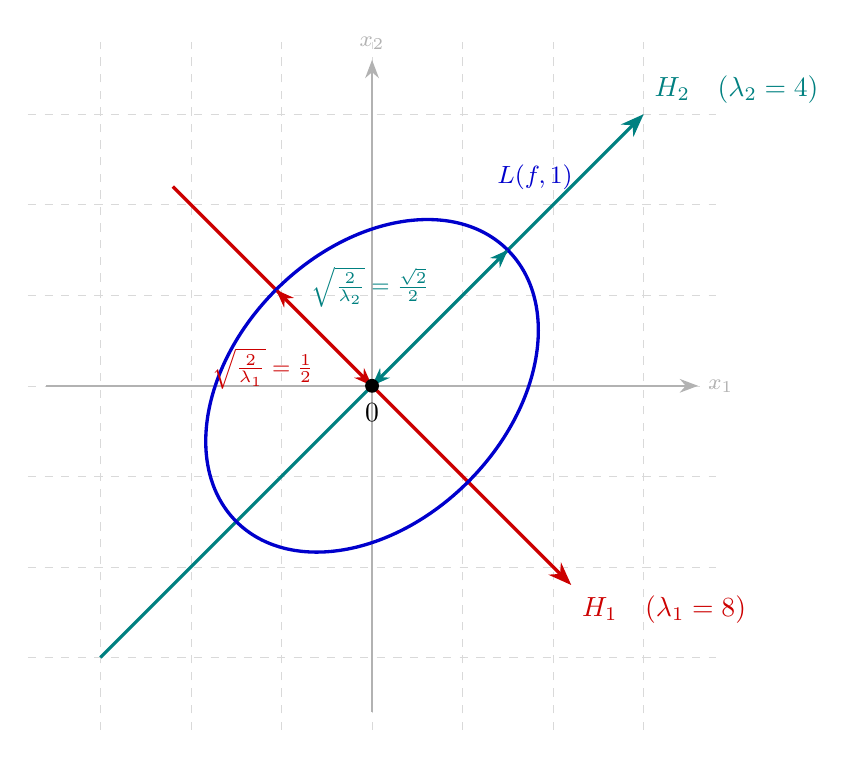
\begin{tikzpicture}[>=Stealth, scale=1.15]
    % Axes
    \draw[help lines, color=gray!30, dashed] (-3.8,-3.8) grid (3.8,3.8);
    \draw[->, thick, gray!60] (-3.6,0) -- (3.6,0) node[right, font=\footnotesize] {$x_1$};
    \draw[->, thick, gray!60] (0,-3.6) -- (0,3.6) node[above, font=\footnotesize] {$x_2$};

    % Rotated coordinate system along eigenvectors H1 and H2
    \draw[->, very thick, teal] (-3.0, -3.0) -- (3.0, 3.0) node[above right] {$H_2 \quad (\lambda_2 = 4)$};
    \draw[->, very thick, red!80!black] (-2.2, 2.2) -- (2.2, -2.2) node[below right] {$H_1 \quad (\lambda_1 = 8)$};

    % Ellipse rotated by 45 degrees
    \draw[very thick, blue!80!black, rotate=45] (0,0) ellipse (2.12cm and 1.5cm);

    % Semi-axis annotations
    \draw[<->, thick, teal] (0,0) -- (1.5, 1.5) node[midway, above left, font=\footnotesize] {$\sqrt{\frac{2}{\lambda_2}} = \frac{\sqrt{2}}{2}$};
    \draw[<->, thick, red!80!black] (0,0) -- (-1.06, 1.06) node[midway, below left, font=\footnotesize] {$\sqrt{\frac{2}{\lambda_1}} = \frac{1}{2}$};

    % Level set label
    \node[blue!80!black, font=\small] at (1.8, 2.3) {$L(f, 1)$};
    \filldraw (0,0) circle (2pt) node[below=3pt] {$0$};
\end{tikzpicture}
\caption{Geometry of level set $L(f, 1)$ for a positive definite matrix: alignment along orthonormal eigenvectors $H_1, H_2$ and inverse semi-axis proportionality.}
\label{fig:ellipsoid-eigenvectors-en}
\end{figure}

\subsection{Degeneration into Open Elliptic Cylinders (\texorpdfstring{$\lambda_i \to 0$}{lambda -> 0})}
As an eigenvalue tends to zero ($\lambda_i \to 0^+$):
\begin{equation}
\lim_{\lambda_i \to 0^+} \text{semi-axis}_i = \lim_{\lambda_i \to 0^+} \sqrt{\frac{2}{\lambda_i}} = +\infty
\end{equation}
In 3D space with $\lambda_1 > 0$, $\lambda_2 > 0$, and $\lambda_3 \to 0^+$, the compact ellipsoid elongates along $H_3$. At the exact limit $\lambda_3 = 0$, the surface opens to infinity, forming a hollow \textbf{elliptic cylinder}.

\subsection{Summary of Level Geometries}
\begin{table}[H]
\centering
\small
\renewcommand{\arraystretch}{1.3}
\begin{tabularx}{\textwidth}{l X X}
\toprule
\textbf{Spectral Regime} & \textbf{Graph Geometry $\text{gr}(f)$} & \textbf{Level Sets $L(f, v)$} \\
\midrule
$Q \succ 0$ & Convex paraboloid & Compact ellipsoids ($v > 0$) \\
$Q \succeq 0$ ($\exists \lambda_i = 0$) & Parabolic trough / gutter & Open elliptic cylinders ($\infty$) \\
$Q \succ\prec 0$ & Hyperbolic paraboloid (Saddle) & One- or two-sheeted hyperboloids \\
$Q \prec 0$ & Inverted concave paraboloid & Compact ellipsoids ($v < 0$) \\
\bottomrule
\end{tabularx}
\caption{Summary of geometric profiles for homogeneous quadratic forms.}
\label{tab:level-geometries-en}
\end{table}


\FloatBarrier
\section{Quadratic Optimization: Unconstrained vs Box-Constrained}
\label{sec:opt-quadratic-unconstrained-vs-box-np-en}

\subsection{Unconstrained Optimization: Immediate Analytical Solution}
For the unconstrained problem:
\begin{equation}
\min_{x \in \R^n} \frac{1}{2} x^T Q x
\end{equation}
spectral analysis provides a complete characterization:
\begin{itemize}
    \item If $Q \succ 0$: unique minimizer $x^* = 0$, $f^* = 0$.
    \item If $Q \succeq 0$: optimal subspace $X^* = \ker(Q)$, $f^* = 0$.
    \item If any eigenvalue is strictly negative ($\lambda_n < 0$): $f^* = -\infty$.
\end{itemize}

\subsection[Box-Constrained Optimization: Complexity Shift]{Box-Constrained Optimization:\\ Complexity Shift and \texorpdfstring{$\mathcal{NP}$}{NP}-Hardness}
Consider the identical objective restricted to a bounded hyper-rectangle:
\begin{equation}
(P_{\text{box}}) \quad \min \left\{ \frac{1}{2} x^T Q x : x \in X = [x_-, x_+] \subset \R^n \right\}
\end{equation}
where $[x_-, x_+] = \{x \in \R^n : x_i^- \le x_i \le x_i^+, \; i = 1, \dots, n\}$.

While univariate box-constrained optimization ($n = 1$) admitted an immediate $\BigO{1}$ solution, in general dimension a dramatic complexity transition occurs:

\begin{enumerate}
    \item \textbf{If $Q \succeq 0$ (Convex Problem):}
    The problem possesses a unique global minimum (or a compact convex set of equivalent minima). It can be solved in polynomial time via interior-point methods or projected gradient algorithms~\cite{boyd2004convex, nocedal2006numerical}. However, \textbf{no closed-form formula exists}: solutions require iterative numerical algorithms.
    
    \item \textbf{If $Q$ is Indefinite ($Q \succ\prec 0$) or Negative Definite ($Q \prec 0$) (Non-Convex Problem):}
    Negative curvature pushes minima to the outer boundary of the feasible domain. Local and global minima reside strictly on the \textbf{vertices of the box}:
    \begin{equation}
    x^* \in \text{vertices}(X) = \prod_{i=1}^n \{x_i^-, x_i^+\}
    \end{equation}
    Since the hypercube possesses $2^n$ vertices, brute-force search is computationally intractable.
\end{enumerate}

\begin{theorem}[Complexity of Box-Constrained QP~\cite{deklerk2008complexity}]
Box-constrained quadratic programming $(P_{\text{box}})$ with a general non-positive semidefinite matrix $Q$ is $\mathcal{NP}$-hard.
\end{theorem}

\begin{alertblock}{The Didactic Paradox of Optimization}
Imposing seemingly trivial coordinate-wise bounds $x_i \in [x_i^-, x_i^+]$ on an elementary quadratic function elevates an instantly solvable problem into the class of $\mathcal{NP}$-hard computational problems.
\end{alertblock}

\chapter[Inhomogeneous Quadratic Optimization and GMQ]{Inhomogeneous Quadratic Optimization,\\Optimality Conditions, and the Gradient Method}
\label{chap:inhomogeneous-quadratic-optimization-gmq}

This chapter extends the study of multivariate quadratic optimization to the general inhomogeneous setting by incorporating a linear term that offsets the center of the function from the origin. We analyze in detail both the non-singular Hessian setting and the singular case, rigorously characterizing the existence of global minima via orthogonal subspace decomposition and linear system compatibility. We formalize the fundamental conceptual bridge connecting numerical linear algebra and continuous optimization, motivating the paradigm shift from direct matrix factorizations to scalable iterative algorithms. Finally, we introduce and analyze the Gradient Method for Quadratic functions (GMQ) equipped with exact line search, proving its convergence properties, operational FLOP cost reduction, and characteristic zig-zag dynamical behavior under varying spectral conditioning.

\FloatBarrier
\section{Inhomogeneous Quadratic Optimization: The Non-Singular Case}
\label{sec:inhomogeneous-quadratic-non-singular}

\subsection{Introduction and Motivation}
In the previous chapter, we investigated purely homogeneous quadratic forms:
\begin{equation}
    f_0(x) = \frac{1}{2} x^T Q x, \quad Q \in \R^{n \times n} \text{ symmetric}.
\end{equation}
Under strict convexity ($Q \succ 0$), this problem admits a unique, trivial global minimizer located precisely at the origin of the vector space:
\begin{equation}
    x^* = 0, \quad f_0(x^*) = 0.
\end{equation}

In real-world data science, engineering, and machine learning models (most notably in linear least squares regression and margin-based classifiers), the center of gravity of the loss function rarely resides at the origin. Introducing a linear term $q^T x$ is required to account for rigid translation:
\begin{equation}
    f(x) = \frac{1}{2} x^T Q x + q^T x, \quad Q = Q^T \in \R^{n \times n}, \; q \in \R^n.
    \label{eq:inhomogeneous-quadratic}
\end{equation}

In this opening analysis, the matrix $Q$ is assumed to be \textbf{non-singular}:
\begin{equation}
    \det(Q) \neq 0 \iff \lambda_i \neq 0 \quad \forall i \in \{1, \dots, n\} \iff \exists Q^{-1}.
\end{equation}
We do not yet require all eigenvalues to share the same sign, but we strictly exclude zero eigenvalues from the spectrum of $Q$.

\subsection{The Multivariate Coordinate Transformation Principle}
To minimize the inhomogeneous function~\eqref{eq:inhomogeneous-quadratic}, we generalize to $n$ dimensions the univariate algebraic principle of completing the square: \textbf{apply a rigid spatial translation} that absorbs the linear term $q^T x$, mapping the objective to a homogeneous quadratic form in $z$.

We define the affine coordinate transformation:
\begin{equation}
    z = x - \bar{x} \iff x = z + \bar{x},
    \label{eq:coord-shift-z}
\end{equation}
where $\bar{x} \in \R^n$ represents the new origin (translation offset) to be determined analytically.

\subsection{Detailed Algebraic Derivation}
Substituting $x = z + \bar{x}$ into $f(x)$ yields:
\begin{equation}
    f(x) = f(z + \bar{x}) = \frac{1}{2} (z + \bar{x})^T Q (z + \bar{x}) + q^T (z + \bar{x}).
\end{equation}

Expanding the bilinear quadratic form using matrix distributivity:
\begin{equation}
    \frac{1}{2} (z + \bar{x})^T Q (z + \bar{x}) = \frac{1}{2} \left( z^T Q z + z^T Q \bar{x} + \bar{x}^T Q z + \bar{x}^T Q \bar{x} \right).
\end{equation}
Because $Q$ is symmetric ($Q = Q^T$), the scalar cross-terms coincide:
\begin{equation}
    z^T Q \bar{x} = (z^T Q \bar{x})^T = \bar{x}^T Q^T z = \bar{x}^T Q z.
\end{equation}
Hence:
\begin{equation}
    \frac{1}{2} (z + \bar{x})^T Q (z + \bar{x}) = \frac{1}{2} z^T Q z + \bar{x}^T Q z + \frac{1}{2} \bar{x}^T Q \bar{x}.
\end{equation}

Expanding the linear term:
\begin{equation}
    q^T (z + \bar{x}) = q^T z + q^T \bar{x}.
\end{equation}

Regrouping terms in powers of $z$:
\begin{equation}
    f(z + \bar{x}) = \frac{1}{2} z^T Q z + \left( \bar{x}^T Q z + q^T z \right) + \left( \frac{1}{2} \bar{x}^T Q \bar{x} + q^T \bar{x} \right).
\end{equation}

\begin{noteblock}{Dimensional Consistency and Factoring}
Tracking vector dimensions: $\bar{x}^T Q$ is a $1 \times n$ row vector, while $z$ is an $n \times 1$ column vector. Factoring $z$ to the right:
\begin{equation}
    \bar{x}^T Q z + q^T z = (Q \bar{x})^T z + q^T z = (Q \bar{x} + q)^T z.
\end{equation}
Furthermore, the sum of constant terms independent of $z$ is precisely the value of the original function evaluated at the translation center $\bar{x}$:
\begin{equation}
    \frac{1}{2} \bar{x}^T Q \bar{x} + q^T \bar{x} = f(\bar{x}).
\end{equation}
\end{noteblock}

Reassembling gives the fundamental translation identity:
\begin{equation}
    f(z + \bar{x}) = \frac{1}{2} z^T Q z + (Q \bar{x} + q)^T z + f(\bar{x}).
    \label{eq:fundamental-translation-identity}
\end{equation}

\subsection{Vanishing Linear Term and Optimal Translation Center}
To ensure that $f(z + \bar{x})$ collapses into a purely homogeneous quadratic form in $z$ plus an additive constant, we enforce that the vector coefficient of the linear term vanishes identically:
\begin{equation}
    Q \bar{x} + q = 0 \iff Q \bar{x} = -q.
\end{equation}

Since $Q$ is non-singular by assumption ($\det(Q) \neq 0$), the matrix inverse $Q^{-1}$ exists and is unique. The optimal center is therefore:
\begin{equation}
    \bar{x} = -Q^{-1} q.
    \label{eq:translation-center-opt}
\end{equation}

Defining the transformed objective $g(z) \coloneqq f(z + \bar{x})$, it takes the canonical form:
\begin{equation}
    g(z) = \frac{1}{2} z^T Q z + f(\bar{x}),
\end{equation}
where the scalar $f(\bar{x}) \in \R$ is an invariant vertical offset that does not alter the location of the minimizer:
\begin{equation}
    \argmin_{z \in \R^n} g(z) = \argmin_{z \in \R^n} \left\{ \frac{1}{2} z^T Q z \right\}.
\end{equation}

\subsection{Optimal Solution and Optimal Value}
From our analysis of homogeneous quadratic forms, if $Q \succ 0$, the unique global minimizer for $z$ is the origin:
\begin{equation}
    z^* = 0.
\end{equation}
Transforming back to the original coordinates $x$ via~\eqref{eq:coord-shift-z}:
\begin{equation}
    x^* = z^* + \bar{x} = 0 + \bar{x} = \bar{x} = -Q^{-1} q.
\end{equation}

The optimal value $f^* \coloneqq f(x^*)$ is evaluated directly:
\begin{equation}
    f^* = f(x^*) = \frac{1}{2} (-Q^{-1} q)^T Q (-Q^{-1} q) + q^T (-Q^{-1} q).
\end{equation}
Using the symmetry of $Q$, we have $(Q^{-1})^T = Q^{-1}$, yielding:
\begin{equation}
    f^* = \frac{1}{2} q^T Q^{-1} Q Q^{-1} q - q^T Q^{-1} q = \frac{1}{2} q^T Q^{-1} q - q^T Q^{-1} q = -\frac{1}{2} q^T Q^{-1} q.
    \label{eq:optimal-value-non-singular}
\end{equation}

\subsection{Full Characterization Across the Spectrum of \texorpdfstring{$Q$}{Q}}
Depending on the eigenvalue signs of non-singular $Q$, three exhaustive regimes emerge:
\begin{enumerate}
    \item \textbf{$Q \succ 0$ (Positive Definite):}
    \begin{itemize}
        \item All eigenvalues are strictly positive ($\lambda_i > 0$).
        \item There exists a \textbf{unique global minimum}: $x^* = -Q^{-1} q$.
        \item The finite optimal objective value is $f^* = -\frac{1}{2} q^T Q^{-1} q$.
        \item The function is unbounded above: $\sup_{x \in \R^n} f(x) = +\infty$.
    \end{itemize}
    \item \textbf{$Q \prec 0$ (Negative Definite):}
    \begin{itemize}
        \item All eigenvalues are strictly negative ($\lambda_i < 0$).
        \item There exists a \textbf{unique global maximum}: $x_{\max}^* = -Q^{-1} q$.
        \item The function is unbounded below: $\inf_{x \in \R^n} f(x) = -\infty$.
    \end{itemize}
    \item \textbf{$Q \succ\prec 0$ (Indefinite):}
    \begin{itemize}
        \item Both positive and negative eigenvalues coexist.
        \item The stationary point $\bar{x} = -Q^{-1} q$ is a \textbf{saddle point}.
        \item The function is unbounded both above and below:
        \begin{equation}
            \inf_{x \in \R^n} f(x) = -\infty, \qquad \sup_{x \in \R^n} f(x) = +\infty.
        \end{equation}
    \end{itemize}
\end{enumerate}


\FloatBarrier
\section{Inhomogeneous Quadratic Optimization: The Singular Case}
\label{sec:inhomogeneous-quadratic-singular}

\subsection{Singularity of \texorpdfstring{$Q$}{Q} and Failure of Direct Inversion}
What occurs when the symmetric matrix $Q$ possesses one or more zero eigenvalues?
\begin{equation}
    \exists i \in \{1, \dots, n\} : \lambda_i = 0 \iff \det(Q) = 0 \iff Q \text{ is singular}.
\end{equation}
In this case, the inverse $Q^{-1}$ does not exist, and the linear system $Q \bar{x} = -q$ cannot be solved by direct matrix inversion.

To characterize the underlying geometry, we partition the spectrum index set $I = \{1, 2, \dots, n\}$ according to eigenvalue vanishing:
\begin{equation}
    I^0 = \{i \in I : \lambda_i = 0\}, \quad k = |I^0| > 0,
\end{equation}
\begin{equation}
    I^+ = \{i \in I : \lambda_i \neq 0\}, \quad h = |I^+| > 0, \quad k + h = n.
\end{equation}

The orthonormal eigenvectors $\{H_i\}_{i=1}^n$ of $Q$ span two fundamental orthogonal subspaces of $\R^n$:
\begin{enumerate}
    \item \textbf{The Kernel (Null Space):}
    \begin{equation}
        \ker(Q) = \{v \in \R^n : Qv = 0\} = \spanop\left(\{H_i\}_{i \in I^0}\right), \quad \dim(\ker(Q)) = k.
    \end{equation}
    \item \textbf{The Image (Range / Column Space):}
    \begin{align}
        \operatorname{im}(Q) &= \{w \in \R^n : \exists x \in \R^n, \; Qx = w\} \nonumber \\
        &= \spanop(\{H_i\}_{i \in I^+}), \quad \dim(\operatorname{im}(Q)) = h.
    \end{align}
\end{enumerate}

Because the spectral basis $H$ is orthonormal, the \textbf{orthogonal decomposition theorem} holds:
\begin{equation}
    \R^n = \operatorname{im}(Q) \oplus \ker(Q), \quad \text{with } \operatorname{im}(Q) \perp \ker(Q).
\end{equation}
Every vector in $\R^n$ decomposes uniquely into the sum of an image component and a kernel component.

\begin{figure}[H]
\centering
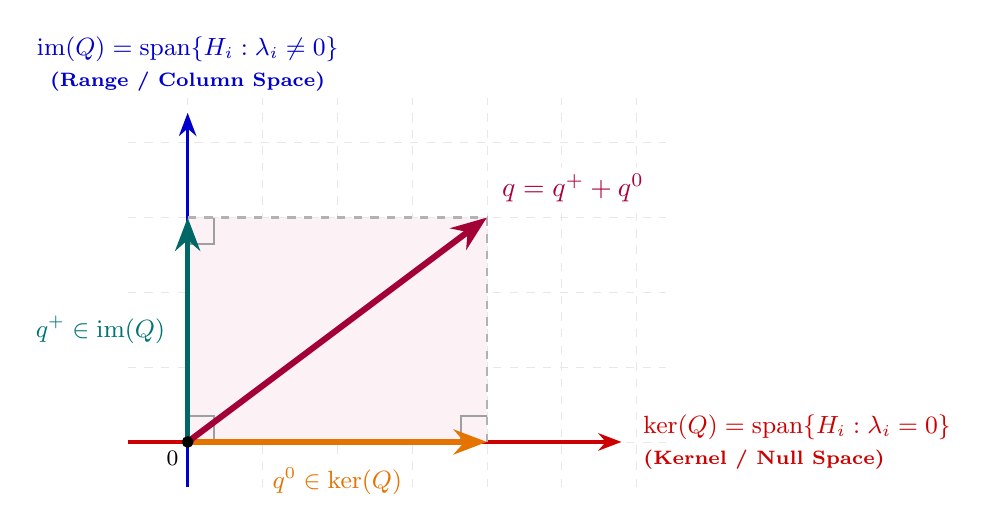
\begin{tikzpicture}[>=Stealth, scale=0.95]
    % Background subtle grid
    \draw[help lines, color=gray!18, dashed] (-0.8, -0.6) grid (6.4, 4.6);

    % Orthogonal Subspaces: im(Q) vertical, ker(Q) horizontal
    \draw[->, very thick, blue!80!black] (0, -0.6) -- (0, 4.4) node[above=4pt, font=\small\bfseries, align=center] {$\operatorname{im}(Q) = \spanop\{H_i : \lambda_i \neq 0\}$\\{\scriptsize (Range / Column Space)}};
    \draw[->, very thick, red!80!black] (-0.8, 0) -- (5.8, 0) node[right=4pt, font=\small\bfseries, align=left] {$\ker(Q) = \spanop\{H_i : \lambda_i = 0\}$\\{\scriptsize (Kernel / Null Space)}};

    % Coordinates of decomposition
    \coordinate (O) at (0, 0);
    \coordinate (Qvec) at (4.0, 3.0);
    \coordinate (Qplus) at (0, 3.0);
    \coordinate (Qzero) at (4.0, 0);

    % Shaded decomposition rectangle
    \fill[purple!5] (O) rectangle (Qvec);

    % Dashed projection lines with distinct color
    \draw[dashed, gray!60, line width=0.9pt] (Qplus) -- (Qvec);
    \draw[dashed, gray!60, line width=0.9pt] (Qzero) -- (Qvec);

    % Right-angle markers at axes and projection corners
    \draw[thick, gray!75] (0, 0.35) -- (0.35, 0.35) -- (0.35, 0);
    \draw[thick, gray!75] (4.0, 0.35) -- (3.65, 0.35) -- (3.65, 0);
    \draw[thick, gray!75] (0.35, 3.0) -- (0.35, 2.65) -- (0, 2.65);

    % Component Vectors (q+ in im(Q), q0 in ker(Q))
    \draw[->, line width=2.0pt, teal!80!black] (O) -- (Qplus);
    \node[left=6pt, fill=white, fill opacity=0.9, text opacity=1, inner sep=2pt, rounded corners=2pt, font=\small\bfseries, text=teal!90!black] at (0, 1.5) {$q^+ \in \operatorname{im}(Q)$};

    \draw[->, line width=2.0pt, orange!90!black] (O) -- (Qzero);
    \node[below=7pt, fill=white, fill opacity=0.9, text opacity=1, inner sep=2pt, rounded corners=2pt, font=\small\bfseries, text=orange!90!black] at (2.0, 0) {$q^0 \in \ker(Q)$};

    % Resultant Vector q = q+ + q0
    \draw[->, line width=2.2pt, purple!85!black] (O) -- (Qvec);
    \node[above right=4pt, fill=white, fill opacity=0.95, text opacity=1, inner sep=2.5pt, rounded corners=3pt, font=\normalsize\bfseries, text=purple!90!black] at (Qvec) {$q = q^+ + q^0$};

    % Origin marker
    \filldraw (O) circle (2pt);
    \node[below left=3pt, fill=white, fill opacity=0.9, text opacity=1, inner sep=1pt, rounded corners=2pt, font=\footnotesize\bfseries] at (O) {$0$};
\end{tikzpicture}
\caption{Orthogonal subspace decomposition $\R^n = \operatorname{im}(Q) \oplus \ker(Q)$: the linear term vector $q$ decomposes uniquely into the sum $q = q^+ + q^0$, with $q^+ \perp q^0$.}
\label{fig:orthogonal-decomposition-q-en}
\end{figure}

\subsection{Functional Competition: Quadratic Term vs Linear Term}
Consider the directional tomography along a direction in the kernel $v \in \ker(Q)$:
\begin{equation}
    f(v) = \frac{1}{2} v^T Q v + q^T v = \frac{1}{2} v^T (0) + q^T v = q^T v.
\end{equation}
Along the null space, the second-order quadratic term vanishes entirely. The function collapses to a \textbf{purely linear scalar map}:
\begin{equation}
    \phi_{0, v}(\alpha) = \alpha (q^T v).
\end{equation}

This property induces a critical structural dilemma:
\begin{itemize}
    \item A non-constant linear function on $\R$ ($\alpha \mapsto c\alpha$ with $c \neq 0$) never attains a minimum, as it tends to $-\infty$ along one ray.
    \item The only mechanism preventing the function from plunging to $-\infty$ along the null space is for the line to be horizontal, which requires:
    \begin{equation}
        q^T v = 0 \quad \forall v \in \ker(Q) \iff q \perp \ker(Q).
    \end{equation}
    \item Because $\operatorname{im}(Q) \perp \ker(Q)$, being orthogonal to the kernel is strictly equivalent to:
    \begin{equation}
        q \in \operatorname{im}(Q).
    \end{equation}
\end{itemize}

\subsection{Decomposition of \texorpdfstring{$q$}{q} and Minimum Existence Conditions}
Decomposing $q$ along the orthogonal components:
\begin{equation}
    q = q^+ + q^0, \quad \text{with } q^+ \in \operatorname{im}(Q), \; q^0 \in \ker(Q), \; q^+ \perp q^0.
\end{equation}

Substituting this into the translated form~\eqref{eq:fundamental-translation-identity}:
\begin{equation}
    f(z + \bar{x}) = \frac{1}{2} z^T Q z + (Q \bar{x} + q^+ + q^0)^T z + f(\bar{x}).
\end{equation}
Since $q^+ \in \operatorname{im}(Q)$, by definition of the image of a linear operator there always exists at least one vector $\bar{x} \in \R^n$ satisfying:
\begin{equation}
    Q \bar{x} = -q^+ \iff Q \bar{x} + q^+ = 0.
\end{equation}
Fixing such an $\bar{x}$, the expression simplifies to:
\begin{equation}
    f(z + \bar{x}) = \frac{1}{2} z^T Q z + (q^0)^T z + f(\bar{x}).
    \label{eq:reduced-singular-form-en}
\end{equation}

Two mutually exclusive, exhaustive scenarios now emerge:

\paragraph{Scenario A: $q^0 \neq 0 \iff q \notin \operatorname{im}(Q)$ (Unbounded Below).}
If $q$ has a non-zero projection onto the null space of $Q$, we choose the direction $d = q^0 \in \ker(Q)$ and move along $z = -\alpha q^0$ with $\alpha > 0$:
\begin{equation}
    g(-\alpha q^0) = \frac{1}{2} (-\alpha q^0)^T Q (-\alpha q^0) + (q^0)^T (-\alpha q^0) + f(\bar{x}).
\end{equation}
Since $Q q^0 = 0$:
\begin{equation}
    g(-\alpha q^0) = 0 - \alpha \|q^0\|^2 + f(\bar{x}).
\end{equation}
Taking the limit as $\alpha \to +\infty$:
\begin{equation}
    \lim_{\alpha \to +\infty} g(-\alpha q^0) = -\infty \implies f^* = -\infty.
\end{equation}
The function is unbounded from below and no minimum exists.

\paragraph{Scenario B: $q^0 = 0 \iff q \in \operatorname{im}(Q)$ (Infinitely Many Global Minima).}
If the kernel component vanishes, the linear system:
\begin{equation}
    Q \bar{x} = -q
\end{equation}
is \textbf{compatible} by the Rouch\'e-Capelli theorem. The translated function~\eqref{eq:reduced-singular-form-en} becomes purely homogeneous:
\begin{equation}
    g(z) = \frac{1}{2} z^T Q z + f(\bar{x}).
\end{equation}
Assuming $Q \succeq 0$ (positive semidefinite):
\begin{itemize}
    \item The minimum of $\frac{1}{2} z^T Q z$ is zero, achieved for every vector $z \in \ker(Q)$.
    \item In original coordinates, the set of global minimizers forms the affine variety:
    \begin{equation}
        X^* = \bar{x} + \ker(Q) = \{x \in \R^n : x = \bar{x} + v, \; v \in \ker(Q)\}.
    \end{equation}
    \item All points in $X^*$ achieve \textbf{precisely the same objective value}:
    \begin{align}
        f(\bar{x} + v) &= \frac{1}{2} (\bar{x} + v)^T Q (\bar{x} + v) + q^T (\bar{x} + v) \nonumber \\
        &= \frac{1}{2} \bar{x}^T Q \bar{x} + q^T \bar{x} + \underbrace{\bar{x}^T Q v}_{= 0} + \underbrace{\frac{1}{2} v^T Q v}_{= 0} + \underbrace{q^T v}_{= 0} \nonumber \\
        &= f(\bar{x}) \quad (\text{since } v \in \ker(Q) \text{ and } q \perp v).
    \end{align}
\end{itemize}

\begin{theorem}[Minimum Existence for Positive Semidefinite Quadratic Functions]
\label{thm:existence-minimum-psd}
Let $f(x) = \frac{1}{2} x^T Q x + q^T x$ with $Q \succeq 0$. The function admits a finite minimum if and only if the linear system $Qx = -q$ is solvable, which holds if and only if $q \in \operatorname{im}(Q)$.
In that case, the set of global minimizers is the affine subspace $X^* = \bar{x} + \ker(Q)$ and the optimal value is $f^* = f(\bar{x}) = -\frac{1}{2} q^T \bar{x}$.
\end{theorem}


\FloatBarrier
\section{Optimality Conditions and the Link to Linear Algebra}
\label{sec:optimality-conditions-linear-algebra}

\subsection{The Gradient of a Quadratic Function}
Computing the gradient vector of $f(x) = \frac{1}{2} x^T Q x + q^T x$ via vector differentiation:
\begin{equation}
    \nabla f(x) = Qx + q.
\end{equation}
The first-order necessary condition for stationarity (which is also sufficient for global optimality when $Q \succeq 0$) requires the gradient to vanish:
\begin{equation}
    \nabla f(x^*) = 0 \iff Q x^* + q = 0 \iff Q x^* = -q.
\end{equation}

\subsection{The Conceptual Bridge Between Linear Algebra and Optimization}
This single algebraic relationship formalizes the core conceptual duality of computational mathematics:
\begin{equation}
    \underbrace{Qx = -q}_{\text{Numerical Linear Algebra}} \iff \underbrace{\min_{x \in \R^n} \left(\frac{1}{2}x^T Qx + q^T x\right)}_{\text{Continuous Optimization}}
\end{equation}
Every symmetric positive semidefinite linear system admits a dual variational characterization as the minimization of an energy functional.

\subsection{Computational Limitations of Direct Methods}
Given this equivalence, why not always employ classic direct methods from numerical linear algebra (Gaussian elimination, $LU$ decomposition, or Cholesky factorization $Q = L L^T$)?

The limitations stem from computational and memory scalability:
\begin{enumerate}
    \item \textbf{Cubic Time Complexity $\BigO{n^3}$:}
    Directly solving a dense linear system of dimension $n$ requires:
    \begin{equation}
        \frac{1}{3} n^3 \text{ FLOPs (Cholesky)} \quad \text{or} \quad \frac{2}{3} n^3 \text{ FLOPs (Gauss/LU)}.
    \end{equation}
    \begin{itemize}
        \item For $n \approx 10^2$: $n^3 = 10^6$ FLOPs $\longrightarrow$ sub-millisecond execution.
        \item For $n \approx 10^4$: $n^3 = 10^{12}$ FLOPs $\longrightarrow$ seconds to minutes.
        \item For $n \approx 10^9$ (modern deep learning models): $n^3 = 10^{27}$ FLOPs $\longrightarrow$ intractable across human civilization timescales.
    \end{itemize}

    \item \textbf{Memory Complexity and Fill-in Phenomena:}
    Even when the coefficient matrix $Q$ is highly sparse (storable in $\BigO{n}$ memory), the triangular factors $L$ generated by Gaussian elimination suffer from \textbf{fill-in} (zero entries transitioning into non-zeros). This destroys structural sparsity and demands $\BigO{n^2}$ memory storage, quickly exhausting system RAM.
\end{enumerate}


\FloatBarrier
\section{Iterative Algorithms and the Gradient Method (GMQ)}
\label{sec:iterative-algorithms-gmq}

\subsection{Philosophy of Iterative Methods}
To overcome the $\BigO{n^3}$ barrier, continuous optimization relies on \textbf{iterative schemes}:
\begin{enumerate}
    \item Select an initial candidate point $x^0 \in \R^n$ (typically $x^0 = 0$).
    \item Define an update map $x^k \to x^{k+1}$ generating a sequence $\{x^k\}_{k=0, 1, 2, \dots}$.
    \item Enforce that the objective sequence forms a \textbf{monotonically decreasing sequence}:
    \begin{equation}
        f(x^{k+1}) < f(x^k) \quad \forall k \ge 0.
    \end{equation}
\end{enumerate}
Since any monotonically non-increasing sequence of real numbers bounded from below is guaranteed to converge, the algorithm converges toward the infimum of the objective.

\subsection{The Residual Vector as a Descent Direction}
Given the current iterate $x^k$, we define the \textbf{residual vector} (which coincides with the instantaneous gradient):
\begin{equation}
    g^k \coloneqq \nabla f(x^k) = Q x^k + q.
\end{equation}

If $\|g^k\| \le \varepsilon$ for a chosen tolerance $\varepsilon > 0$, stationarity is satisfied and the algorithm halts.
If $\|g^k\| > \varepsilon$, we construct the directional tomography along the \textbf{antigradient} $d = -g^k$:
\begin{equation}
    \phi_{x^k, -g^k}(\alpha) = f(x^k - \alpha g^k) - f(x^k).
\end{equation}

Expanding the univariate variation $\phi(\alpha)$:
\begin{align}
    \phi(\alpha) &= \frac{1}{2} (x^k - \alpha g^k)^T Q (x^k - \alpha g^k) + q^T (x^k - \alpha g^k) - \left( \frac{1}{2} (x^k)^T Q x^k + q^T x^k \right) \nonumber \\
    &= \frac{1}{2} \alpha^2 (g^k)^T Q g^k - \alpha (g^k)^T Q x^k - \alpha q^T g^k \nonumber \\
    &= \frac{1}{2} \alpha^2 (g^k)^T Q g^k - \alpha (g^k)^T (Q x^k + q).
\end{align}
Recognizing that $Q x^k + q = g^k$, we arrive at the \textbf{fundamental descent tomography formula}:
\begin{equation}
    \phi_{x^k, -g^k}(\alpha) = \frac{1}{2} \alpha^2 (g^k)^T Q g^k - \alpha \|g^k\|^2.
    \label{eq:tomography-antigradient-en}
\end{equation}

Analyzing the coefficient signs:
\begin{itemize}
    \item For $Q \succ 0$, quadratic curvature is strictly positive: $(g^k)^T Q g^k > 0$.
    \item Because $g^k \neq 0$, the first-order slope is strictly negative: $-\|g^k\|^2 < 0$.
\end{itemize}
For sufficiently small step sizes $\alpha > 0$, the first-order linear term $-\alpha \|g^k\|^2$ dominates over the second-order term $\frac{1}{2} \alpha^2 (g^k)^T Q g^k$. Thus:
\begin{equation}
    \exists \alpha > 0 : \phi_{x^k, -g^k}(\alpha) < 0 \iff f(x^k - \alpha g^k) < f(x^k).
\end{equation}

\begin{noteblock}{Dual Role of the Gradient}
The instantaneous gradient $g^k = Q x^k + q$ fulfills two complementary roles:
\begin{enumerate}
    \item When non-zero, it serves as a \textbf{certificate of non-optimality} of the current state.
    \item It provides an explicit \textbf{constructive descent direction}: stepping along $-g^k$ strictly decreases the objective value.
\end{enumerate}
\end{noteblock}

\subsection{Analytical Optimal Step Size (Exact Line Search)}
Rather than choosing $\alpha$ empirically, we can analytically compute the value $\alpha_k$ that maximizes function reduction by minimizing the convex parabola $\phi(\alpha)$ in~\eqref{eq:tomography-antigradient-en}:
\begin{equation}
    \min_{\alpha > 0} \left\{ \frac{1}{2} \left( (g^k)^T Q g^k \right) \alpha^2 - \left( \|g^k\|^2 \right) \alpha \right\}.
\end{equation}

Differentiating with respect to $\alpha$ and setting the derivative to zero:
\begin{equation}
    \frac{d\phi}{d\alpha} = \alpha (g^k)^T Q g^k - \|g^k\|^2 = 0 \iff \alpha_k = \frac{\|g^k\|^2}{(g^k)^T Q g^k}.
    \label{eq:optimal-stepsize-en}
\end{equation}

\begin{property}[Spectral Bounds on the Step Size]
By the Rayleigh quotient variational characterization for symmetric positive definite matrices:
\begin{equation}
    \lambda_n \le \frac{(g^k)^T Q g^k}{\|g^k\|^2} \le \lambda_1.
\end{equation}
Inverting the inequality shows that the exact step size $\alpha_k$ is strictly bounded by the reciprocal eigenvalues:
\begin{equation}
    \frac{1}{\lambda_1} \le \alpha_k \le \frac{1}{\lambda_n}.
\end{equation}
\end{property}

\subsection{GMQ Algorithm and FLOP Cost Optimization}
The Gradient Method for Quadratic functions (\textbf{GMQ}) formalizes this iterative strategy. Naively implemented, the algorithm appears to require two matrix-vector multiplications per iteration: one for computing the next gradient $Q x^{k+1}$ and another for the denominator form $(g^k)^T Q g^k$. Each multiplication costs $\BigO{n^2}$ FLOPs.

However, via an algebraic identity, the iteration cost reduces to \textbf{a single matrix-vector multiplication}:
\begin{enumerate}
    \item Compute the auxiliary vector:
    \begin{equation}
        v^k = Q g^k \quad [\text{cost: } \BigO{n^2}].
    \end{equation}
    \item The step denominator becomes an inner product:
    \begin{equation}
        (g^k)^T Q g^k = \langle g^k, v^k \rangle \quad [\text{cost: } \BigO{n}].
    \end{equation}
    \item Update the state vector:
    \begin{equation}
        x^{k+1} = x^k - \alpha_k g^k \quad [\text{cost: } \BigO{n}].
    \end{equation}
    \item Recursively update the gradient vector:
    \begin{equation}
        g^{k+1} = Q x^{k+1} + q = Q(x^k - \alpha_k g^k) + q = (Q x^k + q) - \alpha_k Q g^k = g^k - \alpha_k v^k.
    \end{equation}
    This vector update costs only $\BigO{n}$ FLOPs, completely eliminating the need to evaluate $Q x^{k+1}$.
\end{enumerate}

\begin{algorithm}[H]
\caption{Gradient Method for Quadratic Functions (Optimized GMQ)}
\label{alg:optimized-gmq-en}
\KwInput{Matrix $Q = Q^T \succeq 0 \in \R^{n \times n}$, vector $q \in \R^n$, initial guess $x^0 \in \R^n$, tolerance $\varepsilon > 0$, max iterations $K_{\max}$}
\KwOutput{Stationary point $x^* \approx -Q^{-1}q$}
$x \gets x^0$\;
$g \gets Q x + q$\;
$k \gets 0$\;
\While{$\|g\| > \varepsilon$ \textbf{and} $k < K_{\max}$}{
    $v \gets Q g$\; \tcp{Single matrix-vector product per iteration}
    $\alpha \gets \frac{\|g\|^2}{\langle g, v \rangle}$\; \tcp{Exact optimal step size calculation}
    $x \gets x - \alpha g$\; \tcp{State update}
    $g \gets g - \alpha v$\; \tcp{Recursive gradient update}
    $k \gets k + 1$\;
}
\Return{$x$}
\end{algorithm}

When GMQ converges in $K \ll n$ steps, total runtime is $\BigO{K n^2}$ FLOPs, vastly outperforming the $\BigO{n^3}$ cost of direct factorization methods. For sparse matrices with a bounded number of non-zeros per row, each matrix-vector multiplication costs only $\BigO{n}$, lowering the overall complexity to $\BigO{K n}$.


\FloatBarrier
\section{Experimental Analysis and Iterate Dynamics}
\label{sec:experimental-analysis-gmq}

\subsection{Step Geometry and the Zig-Zag Phenomenon}
A fundamental property of exact line search is the \textbf{orthogonality of consecutive gradients}:
\begin{proposition}[Orthogonality of Consecutive Gradients]
At every iteration of GMQ with exact line search:
\begin{equation}
    \langle g^{k+1}, g^k \rangle = 0 \iff g^{k+1} \perp g^k.
\end{equation}
\end{proposition}

\begin{proof}
Using the recursive gradient formula $g^{k+1} = g^k - \alpha_k Q g^k$:
\begin{align}
    \langle g^{k+1}, g^k \rangle &= (g^{k+1})^T g^k = (g^k - \alpha_k Q g^k)^T g^k \nonumber \\
    &= \|g^k\|^2 - \alpha_k (g^k)^T Q g^k.
\end{align}
Substituting the exact step size $\alpha_k = \frac{\|g^k\|^2}{(g^k)^T Q g^k}$:
\begin{equation}
    \langle g^{k+1}, g^k \rangle = \|g^k\|^2 - \frac{\|g^k\|^2}{(g^k)^T Q g^k} (g^k)^T Q g^k = \|g^k\|^2 - \|g^k\|^2 = 0.
\end{equation}
\end{proof}

Geometrically, the trajectory traced by GMQ turns at a \textbf{precise right angle ($90^\circ$)} at each iteration.

\begin{figure}[H]
\centering
\resizebox{0.95\textwidth}{!}{%
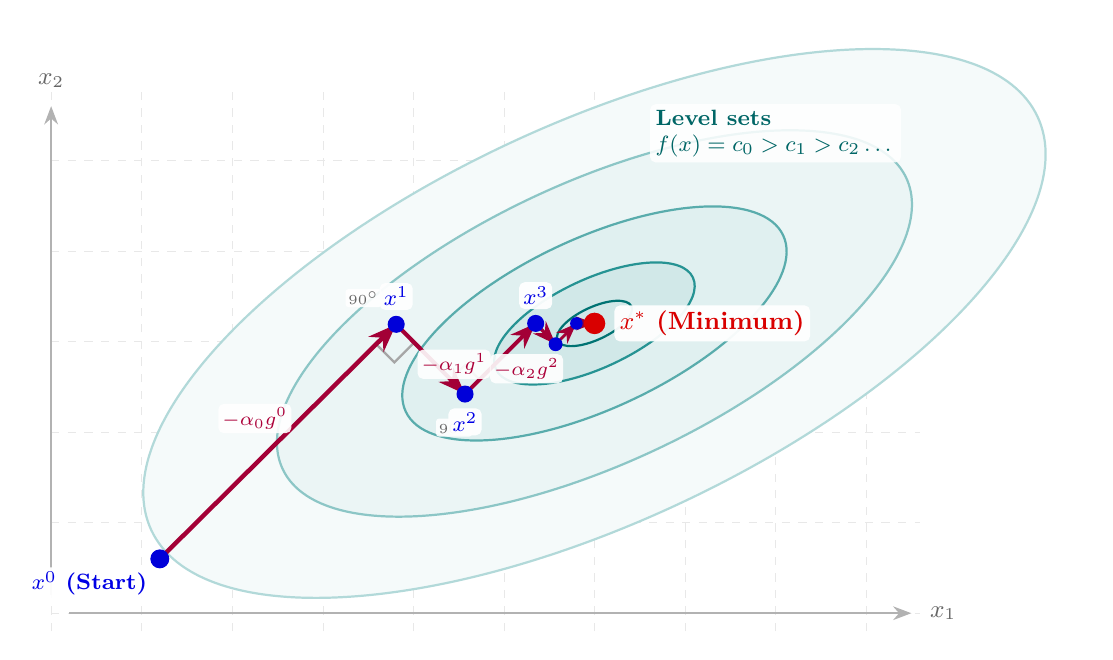
\begin{tikzpicture}[>=Stealth, scale=1.15]
    % Axes and subtle background grid
    \draw[help lines, color=gray!18, dashed] (0, -0.2) grid (9.6, 5.8);
    \draw[->, thick, gray!60] (0.2, 0) -- (9.5, 0) node[right=3pt, font=\small, text=gray!80!black] {$x_1$};
    \draw[->, thick, gray!60] (0, 0.2) -- (0, 5.6) node[above=3pt, font=\small, text=gray!80!black] {$x_2$};

    % Center (minimum): x* = (6.0, 3.2), tilt theta = 25 deg
    % Concentric elliptical level sets with shaded translucent fillings
    \fill[teal!4, rotate around={25:(6.0, 3.2)}] (6.0, 3.2) ellipse (5.40cm and 2.20cm);
    \draw[teal!30, thick, rotate around={25:(6.0, 3.2)}] (6.0, 3.2) ellipse (5.40cm and 2.20cm);

    \fill[teal!8, rotate around={25:(6.0, 3.2)}] (6.0, 3.2) ellipse (3.80cm and 1.55cm);
    \draw[teal!45, thick, rotate around={25:(6.0, 3.2)}] (6.0, 3.2) ellipse (3.80cm and 1.55cm);

    \fill[teal!12, rotate around={25:(6.0, 3.2)}] (6.0, 3.2) ellipse (2.30cm and 0.94cm);
    \draw[teal!65, thick, rotate around={25:(6.0, 3.2)}] (6.0, 3.2) ellipse (2.30cm and 0.94cm);

    \fill[teal!18, rotate around={25:(6.0, 3.2)}] (6.0, 3.2) ellipse (1.20cm and 0.49cm);
    \draw[teal!85, thick, rotate around={25:(6.0, 3.2)}] (6.0, 3.2) ellipse (1.20cm and 0.49cm);

    \draw[teal!90!black, thick, rotate around={25:(6.0, 3.2)}] (6.0, 3.2) ellipse (0.45cm and 0.18cm);

    % Level set callout
    \node[teal!80!black, font=\footnotesize\bfseries, align=left, fill=white, fill opacity=0.85, text opacity=1, inner sep=2pt, rounded corners=2pt] at (8.0, 5.3) {Level sets\\$f(x) = c_0 > c_1 > c_2 \dots$};

    % Mathematically exact GMQ iterate coordinates
    \coordinate (x0) at (1.20, 0.60);
    \coordinate (x1) at (3.81, 3.19);
    \coordinate (x2) at (4.57, 2.42);
    \coordinate (x3) at (5.35, 3.20);
    \coordinate (x4) at (5.57, 2.97);
    \coordinate (x5) at (5.80, 3.20);
    \coordinate (xstar) at (6.00, 3.20);

    % Right-angle markers (showing exact 90-degree orthogonality between consecutive steps)
    \draw[gray!70, thick] ($(x1) + (-0.22, -0.22)$) -- ++(0.20, -0.20) -- ++(0.22, 0.22);
    \node[font=\tiny\bfseries, text=gray!80!black, fill=white, fill opacity=0.9, text opacity=1, inner sep=1pt, rounded corners=1pt] at (3.45, 3.48) {$90^\circ$};

    % Angle at x2 between (x1 -> x2) and (x2 -> x3)
    \draw[gray!70, thick] ($(x2) + (-0.16, 0.16)$) -- ++(0.16, 0.16) -- ++(0.16, -0.16);
    \node[font=\tiny\bfseries, text=gray!80!black, fill=white, fill opacity=0.9, text opacity=1, inner sep=1pt, rounded corners=1pt] at (4.45, 2.05) {$90^\circ$};

    % Descent steps (arrows)
    \draw[->, line width=1.6pt, purple!85!black] (x0) -- (x1);
    \draw[->, line width=1.5pt, purple!85!black] (x1) -- (x2);
    \draw[->, line width=1.4pt, purple!85!black] (x2) -- (x3);
    \draw[->, line width=1.2pt, purple!85!black] (x3) -- (x4);
    \draw[->, line width=1.0pt, purple!85!black] (x4) -- (x5);
    \draw[->, thick, dashed, purple!80!black] (x5) -- (xstar);

    % Descent vector labels (positioned along segments with clean badges)
    \node[fill=white, fill opacity=0.9, text opacity=1, inner sep=1.5pt, rounded corners=2pt, font=\scriptsize\bfseries, text=purple!90!black] at (2.25, 2.15) {$-\alpha_0 g^0$};
    \node[fill=white, fill opacity=0.9, text opacity=1, inner sep=1.5pt, rounded corners=2pt, font=\scriptsize\bfseries, text=purple!90!black] at (4.45, 2.75) {$-\alpha_1 g^1$};
    \node[fill=white, fill opacity=0.9, text opacity=1, inner sep=1.5pt, rounded corners=2pt, font=\scriptsize\bfseries, text=purple!90!black] at (5.25, 2.70) {$-\alpha_2 g^2$};

    % Iterates (points and labels)
    \filldraw[blue!85!black] (x0) circle (2.8pt);
    \node[below left=4pt, fill=white, fill opacity=0.95, text opacity=1, inner sep=1.5pt, rounded corners=2pt, font=\footnotesize\bfseries, text=blue!90!black] at (x0) {$x^0$ (Start)};

    \filldraw[blue!85!black] (x1) circle (2.5pt);
    \node[above=5pt, fill=white, fill opacity=0.95, text opacity=1, inner sep=1.5pt, rounded corners=2pt, font=\footnotesize\bfseries, text=blue!90!black] at (x1) {$x^1$};

    \filldraw[blue!85!black] (x2) circle (2.5pt);
    \node[below=5pt, fill=white, fill opacity=0.95, text opacity=1, inner sep=1.5pt, rounded corners=2pt, font=\footnotesize\bfseries, text=blue!90!black] at (x2) {$x^2$};

    \filldraw[blue!85!black] (x3) circle (2.5pt);
    \node[above=5pt, fill=white, fill opacity=0.95, text opacity=1, inner sep=1.5pt, rounded corners=2pt, font=\footnotesize\bfseries, text=blue!90!black] at (x3) {$x^3$};

    \filldraw[blue!85!black] (x4) circle (2pt);
    \filldraw[blue!85!black] (x5) circle (1.8pt);

    % Global optimum
    \filldraw[red!85!black] (xstar) circle (3.2pt);
    \node[right=7pt, fill=white, fill opacity=0.95, text opacity=1, inner sep=2pt, rounded corners=2pt, font=\small\bfseries, text=red!85!black] at (xstar) {$x^*$ (Minimum)};
\end{tikzpicture}%
}
\caption{Zig-zag trajectory of GMQ across elliptical level sets: exact line search enforces strict orthogonality between successive directions ($\langle g^{k+1}, g^k \rangle = 0$), constraining iterates to turn at exact right angles ($90^\circ$).}
\label{fig:zig-zag-gmq-en}
\end{figure}

\subsection{Experimental Case Studies}
Computational experiments in dimension $n = 2$ reveal how convergence dynamics depend heavily on spectral conditioning:

\subsubsection{Experiment 1: Identity Matrix ($Q = I$)}
Setting $Q = I_2$, eigenvalues coincide: $\lambda_1 = \lambda_2 = 1$. The level sets are perfect circles.
For linear term $q = [10, 5]^T$ and starting point $x^0 = [0, 0]^T$:
\begin{equation}
    g^0 = Q x^0 + q = q = \begin{bmatrix} 10 \\ 5 \end{bmatrix}, \quad \|g^0\|^2 = 125, \quad (g^0)^T Q g^0 = \|g^0\|^2 = 125.
\end{equation}
The optimal step size is $\alpha_0 = 1$. The state update produces:
\begin{equation}
    x^1 = x^0 - 1 \cdot g^0 = \begin{bmatrix} -10 \\ -5 \end{bmatrix}.
\end{equation}
At the next step, $g^1 = Q x^1 + q = [-10, -5]^T + [10, 5]^T = 0$.
The algorithm converges to the exact global minimum in \textbf{1 single iteration}. Geometrically, circular level sets orient the antigradient directly toward the center.

\subsubsection{Experiment 2: Well-Conditioned Matrix ($Q \succ 0$)}
With $Q = \begin{bmatrix} 6 & -2 \\ -2 & 6 \end{bmatrix}$, eigenvalues are $\lambda_1 = 8$ and $\lambda_2 = 4$, with condition number $\kappa(Q) = \lambda_1 / \lambda_2 = 2$.
Level sets are low-eccentricity ellipses. The algorithm produces the typical orthogonal zig-zag trajectory and converges to tolerance $\|g\| \le 10^{-6}$ in only \textbf{12 iterations}.

\subsubsection{Experiment 3: Ill-Conditioned Matrix (Spectral Elongation)}
Decreasing the smallest eigenvalue ($\lambda_2 \to 0^+$), condition number $\kappa(Q)$ grows large. Level sets stretch into elongated ravines.
The $90^\circ$ orthogonality forces iterates to bounce sharply between steep valley walls, producing minute progress along the ravine floor. Iteration counts surge, degrading practical performance.

\subsubsection{Experiment 4: Compatible Singular Matrix ($Q \succeq 0, q \in \operatorname{im}(Q)$)}
With a zero eigenvalue ($\lambda_2 = 0$) and $q$ orthogonal to the null space, an entire affine line of equivalent minima exists. GMQ reduces the gradient norm to the specified tolerance, terminating successfully at the minimizer along the descent path.

\subsubsection{Experiment 5: Incompatible Singular Matrix ($Q \succeq 0, q \notin \operatorname{im}(Q)$)}
When $q$ possesses a non-zero projection onto the null space ($q^0 \neq 0$), objective values plummet monotonically: $f(x^k) \to -\infty$. The gradient norm never reaches zero, remaining bounded away from zero. The algorithm never terminates, faithfully reflecting the unbounded nature of the optimization problem.

\begin{noteblock}{From Experimental Dynamics to Rigorous Convergence Analysis}
The numerical observations from these test cases raise two fundamental open questions:
\begin{enumerate}
    \item \textbf{Quantification of convergence rate:} How does the analytical error contraction factor at each iteration depend on the spectral condition number $\kappa(Q)$?
    \item \textbf{Iteration complexity and singular regime:} How many iterations $k(\epsilon)$ are required to reach a target tolerance $\epsilon$, and what decay law governs convergence when $Q \succeq 0$ loses strict convexity?
\end{enumerate}
These theoretical questions form the core subject of Chapter~\ref{chap:convergence-complexity-gradient-method-quadratics}, where linear convergence is proved via Kantorovich's inequality, asymptotic complexity $\BigO{\kappa(Q) \log(1/\epsilon)}$ is derived in closed form, and sublinear bounds (Bubeck) as well as lower complexity bounds (Nesterov--Nemirovski) are established.
\end{noteblock}

\FloatBarrier
\section{Comparative Synopsis}
\label{sec:comparative-synopsis-quadratic-gmq}

\begin{table}[H]
\centering
\small
\renewcommand{\arraystretch}{1.35}
\begin{tabularx}{\textwidth}{l >{\raggedright\arraybackslash}p{2.6cm} Y >{\raggedright\arraybackslash}p{3.1cm}}
\toprule
\textbf{Matrix Regime $Q$} & \textbf{Condition on $q$} & \textbf{Minimizers $X^*$ and Optimal Value $f^*$} & \textbf{GMQ Dynamical Behavior} \\
\midrule
$Q \succ 0$ & Any $q \in \R^n$ & Unique minimum $x^* = -Q^{-1}q$, $f^* = -\frac{1}{2}q^T Q^{-1}q$ & Linear convergence to $x^*$ (1 step if $Q=I$) \\
$Q \succeq 0$ ($\det Q = 0$) & $q \in \operatorname{im}(Q)$ & Infinitely many minima $X^* = \bar{x} + \ker(Q)$, $f^* = -\frac{1}{2}q^T \bar{x}$ & Converges to a solution in $X^*$ \\
$Q \succeq 0$ ($\det Q = 0$) & $q \notin \operatorname{im}(Q)$ & No minimum ($f^* = -\infty$, unbounded below) & Diverges: $f(x^k) \to -\infty$, $\|g^k\| \not\to 0$ \\
$Q \succ\prec 0$ & Any $q \in \R^n$ & No minimum or maximum (Saddle point) & Does not converge (may diverge depending on $x^0$) \\
$Q \prec 0$ & Any $q \in \R^n$ & Unique maximum, no minimum ($f^* = -\infty$) & Diverges to $-\infty$ along antigradient \\
\bottomrule
\end{tabularx}
\caption{Comprehensive summary of inhomogeneous quadratic optimization and the GMQ algorithm behavior.}
\label{tab:synopsis-quadratic-gmq-en}
\end{table}

\chapter[Convergence and Complexity Analysis of the Gradient Method]{Convergence and Complexity Analysis\\of the Gradient Method for Quadratic Functions}
\label{chap:convergence-complexity-gradient-method-quadratics}

This chapter investigates the theoretical, computational, and empirical performance of the Gradient Method with exact line search (\textit{Steepest Descent}) applied to the unconstrained minimization of multivariate quadratic functions:
\begin{equation}
    f(x) = \frac{1}{2} x^T Q x + q^T x, \quad Q = Q^T \in \R^{n \times n}, \; q \in \R^n.
\end{equation}
The discussion is organized into two primary theoretical parts. In the first part, we examine the strictly convex regime ($Q \succ 0$), formalizing the linear decay of the absolute objective error and deriving the theoretical rate of contraction via the Kantorovich inequality. This highlights the unifying role of the spectral condition number $\kappa(Q)$ and the spatial dimension independence of the algorithm. In the second part, we explore algorithmic complexity theory, comparing the output and input spaces, classifying asymptotic convergence rates (sublinear, linear, superlinear, and quadratic), and rigorously analyzing the singular positive semidefinite regime ($Q \succeq 0, \lambda_n = 0$), Bubeck's $\BigO{1/\epsilon}$ sublinear bound, and the computational detection of unbounded problems ($f^* = -\infty$).

\FloatBarrier
\section{Iterative Algorithms and Minimizing Sequences}
\label{sec:iterative-algorithms-minimizing-sequences}

\subsection{From Direct Solvers to Iterative Schemes}
As analyzed in Chapter~\ref{chap:inhomogeneous-quadratic-optimization-gmq} (Section~\ref{sec:optimality-conditions-linear-algebra}), minimizing the quadratic function $f(x) = \frac{1}{2} x^T Q x + q^T x$ is formally equivalent to solving the symmetric linear system $Q x = -q$. Classical direct numerical methods (Gaussian elimination, Cholesky factorization $Q = L L^T$) exhibit a computational complexity of:
\begin{equation}
    T_{\text{direct}}(n) \in \BigO{n^3} \text{ FLOPs},
\end{equation}
further burdened by matrix fill-in during factorization, which destroys data sparsity and requires $\BigO{n^2}$ memory allocations. For large-scale machine learning and data science problems ($n \ge 10^4$ or $n \ge 10^6$), direct methods become intractable.

Iterative algorithms circumvent this obstacle through low-cost atomic operations, relying solely on matrix-vector products $Q v$ costing $\BigO{n^2}$ (which reduces to $\BigO{n}$ for sparse matrices), generating a sequence of iterates $\{x_k\}$ that systematically converges to the optimum.

\subsection{Fundamental Definitions}

\begin{definition}[Iterative Optimization Algorithm]
An iterative process begins with an initial estimate $x_0 \in \R^n$ (commonly chosen as $x_0 = 0$) and generates an infinite sequence of iterates:
\begin{equation}
    \{x_k\}_{k=0}^\infty \subset \R^n \quad \text{via a transition update } x_k \rightsquigarrow x_{k+1},
\end{equation}
with the goal of driving the sequence toward a minimizer $x^*$.
\end{definition}

\begin{definition}[Minimizing Sequence]
The sequence of objective function values along the iterate path, defined by $f_k = f(x_k)$, is called a \textbf{minimizing sequence} if:
\begin{equation}
    \lim_{k \to \infty} f(x_k) = f^* \equiv \inf_{x \in \R^n} f(x).
\end{equation}
If the problem is unbounded below ($f^* = -\infty$), the sequence satisfies $\lim_{k \to \infty} f(x_k) = -\infty$.
\end{definition}

\begin{definition}[Descent Method (Monotone Algorithm)]
An iterative algorithm is strictly \textbf{monotone decreasing} (or a descent method) if it guarantees a strict objective reduction at every non-stationary step:
\begin{equation}
    f(x_{k+1}) < f(x_k) \quad \forall k \text{ such that } \nabla f(x_k) \neq 0.
\end{equation}
\end{definition}

\begin{proposition}[Existence of the Limit for Minimizing Sequences]
Since every sequence of real numbers $\{f(x_k)\}$ that is strictly monotonically decreasing and bounded below by $f^* > -\infty$ admits a finite limit by the monotone convergence theorem, the descent property guarantees that $\lim_{k \to \infty} f(x_k)$ always exists.
\end{proposition}

\begin{noteblock}{Output Space vs. Input Space Convergence}
Does function value convergence in the output space ($f(x_k) \to f^*$) guarantee iterate convergence in the input space ($x_k \to x^*$)?
\begin{itemize}
    \item \textbf{When $Q \succ 0$ (strictly convex):} Yes. Sublevel sets $\{x \in \R^n \mid f(x) \le f(x_0)\}$ are compact ellipsoids, ensuring that value convergence implies geometric iterate convergence to the unique global minimum $x^*$.
    \item \textbf{When $Q \succeq 0$ with zero eigenvalues or in general non-convex settings:} Not necessarily. Null curvature directions allow iterates to drift indefinitely while objective values remain virtually unchanged.
\end{itemize}
\end{noteblock}

\FloatBarrier
\section{The GMQ Method and Core Geometric Properties}
\label{sec:gradient-method-exact-line-search}

In Chapter~\ref{chap:inhomogeneous-quadratic-optimization-gmq} (Sections~\ref{sec:iterative-algorithms-gmq} and~\ref{sec:experimental-analysis-gmq}), the Gradient Method for Quadratic functions (\textbf{GMQ}) with exact line search was formulated and analyzed. We summarize here the key analytical and operational properties established there, which form the starting point for convergence and complexity analysis:
\begin{enumerate}
    \item \textbf{Direction of steepest descent:} Starting from $x_k \in \R^n$, iterates proceed along the negative instantaneous gradient $g_k \equiv \nabla f(x_k) = Q x_k + q$:
    \begin{equation}
        d_k = -g_k, \quad x_{k+1} = x_k - \alpha_k g_k, \quad \alpha_k > 0.
    \end{equation}
    \item \textbf{Closed-form optimal step size:} Minimizing the univariate parabolic section along the search ray yields the exact step size:
    \begin{equation}
        \alpha_k = \frac{\|g_k\|^2}{g_k^T Q g_k}, \quad \text{with } \frac{1}{\lambda_1} \le \alpha_k \le \frac{1}{\lambda_n},
        \label{eq:optimal-step-size-en}
    \end{equation}
    bounded by the extremal eigenvalues of $Q$ via the Rayleigh quotient characterization for symmetric positive definite matrices.
    \item \textbf{Strict orthogonality of consecutive gradients:} Line search optimality enforces orthogonality between successive gradients:
    \begin{equation}
        \langle g_{k+1}, g_k \rangle = g_{k+1}^T g_k = 0 \quad \forall k \ge 0.
    \end{equation}
    This geometric constraint forces iterates to execute sharp $90^\circ$ turns at every iteration, producing the characteristic zig-zag trajectory illustrated in Figure~\ref{fig:zig-zag-gmq-en} of Chapter~\ref{chap:inhomogeneous-quadratic-optimization-gmq}.
    \item \textbf{Recursive gradient update at $\BigO{n}$ cost:} The update $x_{k+1} = x_k - \alpha_k g_k$ yields the recursive relation:
    \begin{equation}
        g_{k+1} = Q(x_k - \alpha_k g_k) + q = g_k - \alpha_k Q g_k = g_k - \alpha_k v_k, \quad \text{where } v_k \coloneqq Q g_k.
        \label{eq:gradient-update-en}
    \end{equation}
    By caching $v_k$, both the step denominator $\langle g_k, v_k \rangle$ and the updated gradient $g_{k+1}$ are obtained with only $\BigO{n}$ FLOPs, limiting overall complexity to \textbf{a single matrix-vector product per iteration} (Algorithm~\ref{alg:optimized-gmq-en}).
\end{enumerate}

With these algebraic and algorithmic foundations established, we proceed directly to the quantitative analysis of error decay and convergence rates.

\FloatBarrier
\section{Homogeneous Error Representation and Decay}
\label{sec:homogeneous-error-decay}

\subsection{Absolute Objective Function Error}
Assuming $Q \succ 0$, the unique global minimizer satisfies $Q x^* + q = 0 \iff x^* = -Q^{-1}q$. Evaluating the function at $x^*$:
\begin{equation}
    f(x^*) = \frac{1}{2} (x^*)^T Q x^* + q^T x^* = -\frac{1}{2} (x^*)^T Q x^*.
\end{equation}
Define the \textbf{absolute objective error}:
\begin{equation}
    A(x) \equiv f(x) - f(x^*) \ge 0.
\end{equation}
Expanding the difference:
\begin{equation}
    A(x) = \frac{1}{2} x^T Q x + q^T x + \frac{1}{2} (x^*)^T Q x^* = \frac{1}{2} x^T Q x - x^T Q x^* + \frac{1}{2} (x^*)^T Q x^*.
\end{equation}
Recognizing the matrix binomial square:
\begin{equation}
    A(x) = \frac{1}{2} (x - x^*)^T Q (x - x^*).
    \label{eq:error-homogeneous-en}
\end{equation}
Moreover, since $g(x) = Q(x - x^*)$, inverting yields $x - x^* = Q^{-1} g(x)$. Substituting into~\eqref{eq:error-homogeneous-en}:
\begin{equation}
    A(x) = \frac{1}{2} (Q^{-1} g(x))^T Q (Q^{-1} g(x)) = \frac{1}{2} g(x)^T Q^{-1} g(x).
    \label{eq:error-gradient-dual-en}
\end{equation}

\subsection{Exact Recurrence Relation of the Error}
Evaluating $a_{k+1} \equiv A(x_{k+1})$ in terms of $a_k \equiv A(x_k)$:
\begin{align}
    a_{k+1} &= \frac{1}{2} [(x_k - x^*) - \alpha_k g_k]^T Q [(x_k - x^*) - \alpha_k g_k] \nonumber \\
            &= \frac{1}{2} (x_k - x^*)^T Q (x_k - x^*) - \alpha_k g_k^T Q (x_k - x^*) + \frac{1}{2} \alpha_k^2 (g_k^T Q g_k).
\end{align}
Because $Q(x_k - x^*) = g_k$, the middle term simplifies to $g_k^T g_k = \|g_k\|^2$:
\begin{equation}
    a_{k+1} = a_k - \alpha_k \|g_k\|^2 + \frac{1}{2} \alpha_k^2 (g_k^T Q g_k).
\end{equation}
Substituting $\alpha_k = \frac{\|g_k\|^2}{g_k^T Q g_k}$:
\begin{equation}
    a_{k+1} = a_k - \frac{1}{2} \frac{\|g_k\|^4}{g_k^T Q g_k}.
\end{equation}
Dividing and multiplying by $a_k = \frac{1}{2} g_k^T Q^{-1} g_k$:
\begin{equation}
    a_{k+1} = a_k \left[ 1 - \frac{\|g_k\|^4}{(g_k^T Q g_k)(g_k^T Q^{-1} g_k)} \right].
    \label{eq:error-exact-recurrence-en}
\end{equation}
This fundamental identity captures the exact contraction factor at each step.

\FloatBarrier
\section{Kantorovich Inequality and Linear Convergence Rate}
\label{sec:kantorovich-linear-convergence}

\subsection{Spectral Condition Number}
Let $Q \in \R^{n \times n}$ be symmetric positive definite ($Q \succ 0$) with ordered eigenvalues $\lambda_1 \ge \dots \ge \lambda_n > 0$.

\begin{definition}[Spectral Condition Number]
The spectral condition number of $Q$ is defined as:
\begin{equation}
    \kappa(Q) = \frac{\lambda_1}{\lambda_n} = \frac{\lambda_{\max}(Q)}{\lambda_{\min}(Q)} \ge 1.
\end{equation}
\end{definition}

\subsection{Kantorovich Inequality}

\begin{theorem}[Kantorovich Inequality~\cite{nocedal2006numerical}]
\label{thm:kantorovich-en}
Let $Q \in \R^{n \times n}$ be symmetric positive definite with maximum eigenvalue $\lambda_1$ and minimum eigenvalue $\lambda_n$. For every non-zero vector $y \in \R^n \setminus \{0\}$:
\begin{equation}
    \frac{\|y\|^4}{(y^T Q y)(y^T Q^{-1} y)} \ge \frac{4 \lambda_1 \lambda_n}{(\lambda_1 + \lambda_n)^2}.
    \label{eq:kantorovich-inequality-en}
\end{equation}
\end{theorem}

\subsection{Derivation of the Theoretical Convergence Rate}
Applying Theorem~\ref{thm:kantorovich-en} to recurrence~\eqref{eq:error-exact-recurrence-en} with $y = g_k$:
\begin{equation}
    1 - \frac{\|g_k\|^4}{(g_k^T Q g_k)(g_k^T Q^{-1} g_k)} \le 1 - \frac{4 \lambda_1 \lambda_n}{(\lambda_1 + \lambda_n)^2} = \left( \frac{\lambda_1 - \lambda_n}{\lambda_1 + \lambda_n} \right)^2.
\end{equation}
Dividing numerator and denominator by $\lambda_n$ yields the rate expressed in terms of $\kappa = \lambda_1 / \lambda_n$:
\begin{equation}
    r = \left( \frac{\kappa - 1}{\kappa + 1} \right)^2 < 1.
    \label{eq:kantorovich-rate-en}
\end{equation}

\begin{theorem}[Global Linear Convergence of the Gradient Method for $Q \succ 0$]
Let $f(x) = \frac{1}{2} x^T Q x + q^T x$ with $Q \succ 0$. The exact line search gradient method satisfies:
\begin{equation}
    A(x_{k+1}) \le \left( \frac{\kappa - 1}{\kappa + 1} \right)^2 A(x_k),
\end{equation}
implying global geometric decay:
\begin{equation}
    f(x_k) - f(x^*) \le \left( \frac{\kappa - 1}{\kappa + 1} \right)^{2k} (f(x_0) - f(x^*)).
\end{equation}
\end{theorem}

\subsection{Geometric Interpretation of Extreme Cases}
\begin{itemize}
    \item \textbf{Isotropic Ideal Case ($\kappa = 1$):}
    All eigenvalues are equal: $\lambda_1 = \dots = \lambda_n$. The matrix is a scalar multiple of the identity ($Q = \lambda I$). Level curves are perfect hyperspheres. Substituting $\kappa = 1$:
    \begin{equation}
        r = \left( \frac{1 - 1}{1 + 1} \right)^2 = 0 \implies A(x_1) \le 0 \cdot A(x_0) = 0.
    \end{equation}
    The algorithm converges to the exact minimizer in \textbf{1 single iteration} from any starting point $x_0$.
    \item \textbf{Ill-Conditioned Case ($\kappa \gg 1$):}
    Level curves are elongated ellipsoids. As $\kappa \to \infty$, $r \to 1^-$:
    \begin{equation}
        r \approx \left( 1 - \frac{2}{\kappa} \right)^2 \approx 1 - \frac{4}{\kappa}.
    \end{equation}
    Each iteration eliminates only a small fraction ($\approx 4/\kappa$) of error, inducing severe orthogonal oscillations.
\end{itemize}

\FloatBarrier
\section{Computational Complexity and Convergence Rates}
\label{sec:computational-complexity-convergence-rates}

\subsection[Derivation of the Iteration Bound O(log(1/epsilon))]{Derivation of the Iteration Bound $\BigO{\log(1/\epsilon)}$}
Assuming linear error contraction $v_k \le r^k v_0$ with $v_0 = A(x_0)$ and $r < 1$, we find the number of iterations $k$ required to reach tolerance $\epsilon > 0$:
\begin{equation}
    r^k v_0 \le \epsilon \iff k \ge \frac{\ln(v_0 / \epsilon)}{\ln(1/r)}.
\end{equation}
Under ill-conditioning ($r \to 1^-$), using $\ln(1 + \delta) \approx \delta$ with $\delta = (1-r)/r$:
\begin{equation}
    \frac{1}{\ln(1/r)} \approx \frac{r}{1 - r}.
\end{equation}
Hence, iteration complexity scales as:
\begin{equation}
    k \in \BigO{\frac{r}{1 - r} \ln\left( \frac{v_0}{\epsilon} \right)} = \BigO{\kappa(Q) \log\left( \frac{1}{\epsilon} \right)}.
\end{equation}

\subsection{Taxonomy of Asymptotic Convergence Rates}

\begin{definition}[Asymptotic Order and Rate of Convergence]
Let $\{e_k\}_{k=0}^\infty$ denote the error sequence $e_k = f(x_k) - f^* \ge 0$. The order of convergence $p \ge 1$ and asymptotic rate $r > 0$ are given by:
\begin{equation}
    \lim_{k \to \infty} \frac{e_{k+1}}{e_k^p} = r.
\end{equation}
\end{definition}

\begin{table}[H]
\centering
\footnotesize
\renewcommand{\arraystretch}{1.3}
\begin{tabularx}{\textwidth}{l c c X c}
\toprule
\textbf{Regime} & \textbf{Order $p$} & \textbf{Rate $r$} & \textbf{Decay Law} & \textbf{Complexity $k(\epsilon)$} \\
\midrule
\textbf{Sublinear (Slow)}    & $p = 1$ & $r = 1$ & $e_k \approx \BigO{1/k}$          & $\BigO{1/\epsilon}$ \\
\textbf{Sublinear (Nesterov)} & $p = 1$ & $r = 1$ & $e_k \approx \BigO{1/k^2}$        & $\BigO{1/\sqrt{\epsilon}}$ \\
\textbf{Sublinear (Stochastic)} & $p = 1$ & $r = 1$ & $e_k \approx \BigO{1/\sqrt{k}}$ & $\BigO{1/\epsilon^2}$ \\
\textbf{Linear}               & $p = 1$ & $r < 1$ & $e_k \le r^k e_0$                 & $\BigO{\log(1/\epsilon)}$ \\
\textbf{Superlinear}          & $1 < p < 2$ & $r > 0$ & $e_k \approx r^{k^p}$           & Intermediate \\
\textbf{Quadratic (Newton)}   & $p = 2$ & $r > 0$ & $e_k \approx r^{2^k}$             & $\BigO{\log(\log(1/\epsilon))}$ \\
\bottomrule
\end{tabularx}
\caption{Taxonomy of convergence regimes in continuous optimization algorithms.}
\label{tab:convergence-regimes-en}
\end{table}

\begin{itemize}
    \item \textbf{Sublinear ($p=1, r=1$):} The ratio $e_{k+1}/e_k \to 1$. Gaining an extra decimal digit of precision requires multiplying iteration count by 10 (for $1/k$) or 100 (for $1/\sqrt{k}$).
    \item \textbf{Linear ($p=1, r<1$):} Appears as a downward straight line on semi-logarithmic plots ($\log(\text{error})$ vs $k$). Gaining an extra digit of precision adds a fixed constant number of iterations.
    \item \textbf{Quadratic ($p=2$):} The number of correct decimal digits \textbf{doubles at each iteration} ($1 \to 2 \to 4 \to 8 \to 16$), reaching machine precision within 5--8 steps.
\end{itemize}

\FloatBarrier
\section[The Singular Semidefinite Regime (Q >= 0)]{The Singular Semidefinite Regime ($Q \succeq 0$)}
\label{sec:singular-semidefinite-regime}

\subsection{Loss of Strict Convexity and Infinite Conditioning}
When $Q$ is singular ($\det(Q) = 0$), its minimum eigenvalue vanishes: $\lambda_n = 0$. The theoretical condition number becomes infinite:
\begin{equation}
    \kappa(Q) = \frac{\lambda_1}{0} = +\infty \implies r = \left( \frac{\infty - 1}{\infty + 1} \right)^2 = 1.
\end{equation}
The Kantorovich bound yields $A(x_{k+1}) \le 1 \cdot A(x_k)$, providing no guarantee of geometric contraction.

\subsection{Bubeck's Sublinear Convergence Theorem}

\begin{theorem}[Sublinear Bound for Singular Matrices~\cite{bubeck2015convex}]
\label{thm:bubeck-sublinear-en}
Let $f(x) = \frac{1}{2} x^T Q x + q^T x$ with $Q \succeq 0$ symmetric positive semidefinite and $q \in \operatorname{im}(Q)$. Under the gradient method with exact line search (or constant step size $\alpha = 1/\lambda_1$):
\begin{equation}
    f(x_k) - f^* \le \frac{2 \lambda_1 \|x_0 - x^*\|^2}{k - 1}, \quad \forall k \ge 2,
    \label{eq:bubeck-bound-en}
\end{equation}
where $\lambda_1 = \lambda_{\max}(Q)$ and $x^*$ is an optimal solution.
\end{theorem}

Solving for the number of iterations to achieve $f(x_k) - f^* \le \epsilon$:
\begin{equation}
    k \ge 1 + \frac{2 \lambda_1 \|x_0 - x^*\|^2}{\epsilon} \implies k \in \BigO{\frac{1}{\epsilon}}.
\end{equation}
Complexity severely degrades from logarithmic to inverse linear:
\begin{itemize}
    \item Reaching $\epsilon = 10^{-3}$ requires $\approx 10^3$ iterations;
    \item Reaching $\epsilon = 10^{-6}$ requires over $10^6$ iterations, rendering standard gradient descent intractable for high-precision demands.
\end{itemize}

\FloatBarrier
\section{Computational Detection of Unbounded Problems}
\label{sec:detection-unbounded-problems}

\subsection{Algebraic Conditions for Unboundedness Below}
As established in Chapter~\ref{chap:inhomogeneous-quadratic-optimization-gmq} (Section~\ref{sec:inhomogeneous-quadratic-singular} and Theorem~\ref{thm:existence-minimum-psd}), when $Q \succeq 0$ is singular, the space decomposes as $\R^n = \operatorname{im}(Q) \oplus \ker(Q)$. Decomposing the linear term $q = q^+ + q^0$:
\begin{itemize}
    \item \textbf{If $q^0 = 0 \iff q \in \operatorname{im}(Q)$:} The system $Q x = -q$ is consistent, admitting the affine manifold of solutions $X^* = x^* + \ker(Q)$ with finite minimum $f^* = -\frac{1}{2} q^T x^*$;
    \item \textbf{If $q^0 \neq 0 \iff q \notin \operatorname{im}(Q)$:} The system is inconsistent. Along direction $d = -q^0 \in \ker(Q)$, the quadratic term vanishes ($d^T Q d = 0$) while the linear term strictly decreases ($q^T d = -\|q^0\|^2 < 0$), causing the objective to diverge to $-\infty$.
\end{itemize}
While this failure mode corresponds algebraically to system inconsistency, computationally it is imperative that the iterative algorithm detects unboundedness promptly to prevent non-terminating loops or arithmetic overflow.

\subsection{Algorithmic Check in GMQ}
In efficient implementations (such as \texttt{GMQ.m}), unboundedness is caught by examining the step denominator:
\begin{lstlisting}[style=code,caption={Numerical unboundedness detection in GMQ.}]
v = Q * g;
den = g' * v; % computes g_k' * Q * g_k

if den <= 1e-14
    fprintf('g'' * Q * g = %1.4e ==> unbounded\n', den);
    status = 'unbounded';
    break;
end
\end{lstlisting}
This check simultaneously identifies:
\begin{enumerate}
    \item $g_k^T Q g_k \approx 0$ with $\|g_k\| > 0$: The gradient lies in $\ker(Q)$, leading to linear divergence $f \to -\infty$;
    \item $g_k^T Q g_k < 0$: The matrix $Q$ has negative curvature, producing a concave parabola diverging to $-\infty$.
\end{enumerate}

\FloatBarrier
\section{Lower Complexity Bounds and Future Directions}
\label{sec:lower-complexity-bounds}

The slow convergence of gradient descent in singular ($\BigO{1/\epsilon}$) or ill-conditioned ($\BigO{\kappa \log(1/\epsilon)}$) problems prompts an essential theoretical question: is this an algorithm shortcoming or an intrinsic problem barrier?

\textbf{Nesterov and Nemirovski's lower complexity theorems}~\cite{nesterov2004introductory} demonstrate that:
\begin{itemize}
    \item For general convex functions with Lipschitz gradients, no first-order method can converge faster than:
    \begin{equation}
        f(x_k) - f^* \ge \frac{3 L \|x_0 - x^*\|^2}{32 (k + 1)^2} \implies k \in \Omega\left(\frac{1}{\sqrt{\epsilon}}\right);
    \end{equation}
    \item For strongly convex quadratics ($Q \succ 0$), the first-order lower bound scales as:
    \begin{equation}
        k \in \Omega\left(\sqrt{\kappa(Q)} \log\left(\frac{1}{\epsilon}\right)\right).
    \end{equation}
\end{itemize}
Standard gradient descent exhibits a linear dependency on $\kappa(Q)$. This gap motivates momentum and accelerated first-order methods (such as the \textbf{Conjugate Gradient Method}), which preserve an $\BigO{n^2}$ per-iteration matrix-vector cost while accelerating condition number dependency from $\kappa$ to $\sqrt{\kappa}$.


\begingroup
\sloppy
\hbadness=10000
\bibliographystyle{unsrt}
\bibliography{references}
\endgroup

\end{document}
